\documentclass[letterpaper,12pt, twopage]{report}
\usepackage[utf8]{inputenc}
\usepackage[spanish]{babel}
\usepackage{graphicx}
\usepackage{anysize}
\usepackage{float}
\usepackage{fancyhdr}
\usepackage{longtable}
\usepackage{hyperref}
\usepackage{listings}
\usepackage{ragged2e}
\usepackage{verbatim}
\usepackage{pdfpages}

%Agregar aquí los paquetes que hagan falta para su trabajo

\marginsize{4cm}{2.5cm}{4cm}{2.5cm}
\graphicspath{ {figuras/} }

\pagestyle{fancy}
\fancyhf{}

\title{Machine Learning aplicado al QSAR para fármacos} %Cambiar según el título de su tesis


\makeatletter 
\let\newtitle\@title
\let\newauthor\@author
\makeatother

\AtBeginDocument{\renewcommand{\contentsname}{Contenido}}
\AtBeginDocument{\renewcommand{\listtablename}{Índice de tablas}}
\AtBeginDocument{\renewcommand{\tablename}{Tabla}}
\begin{document}
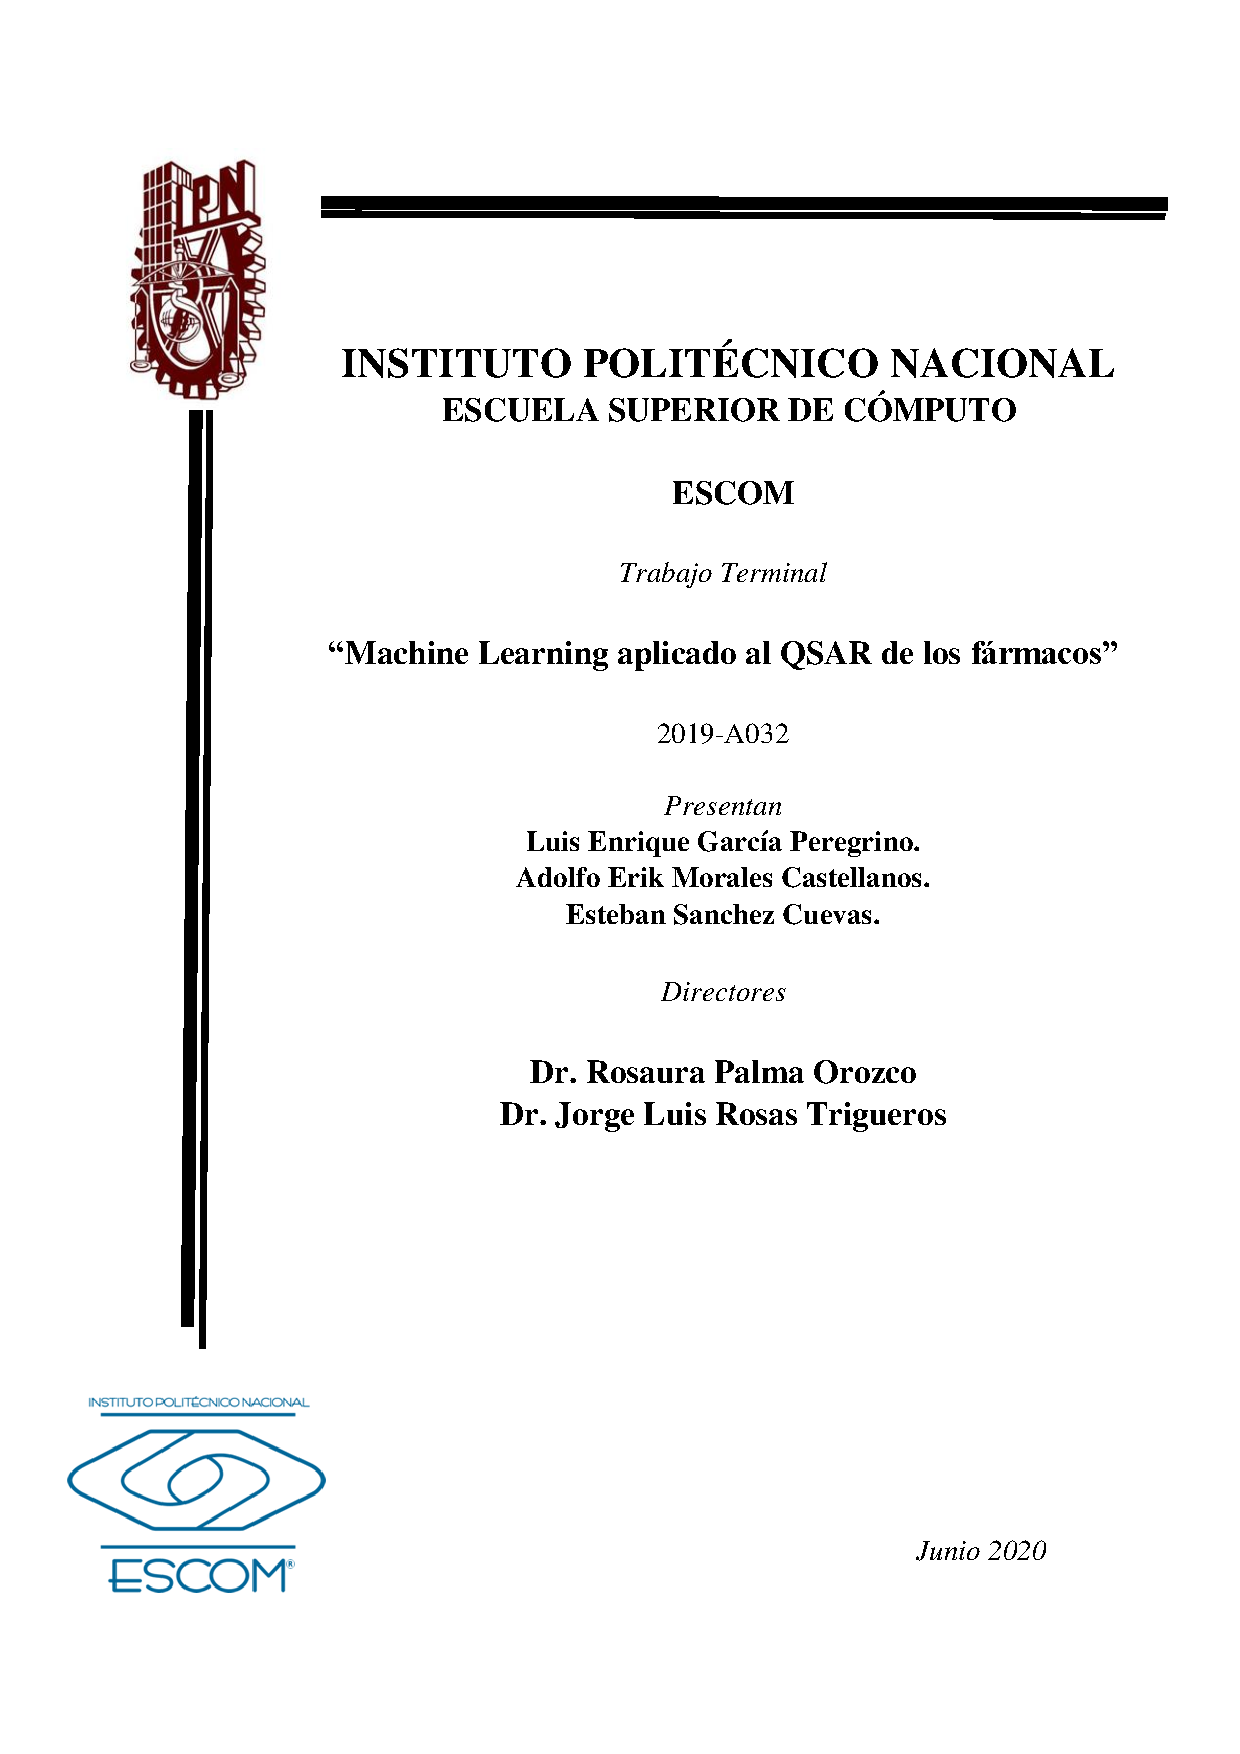
\includepdf[pages=1-1]{Anexo/PortadaTT2}
%%\thispagestyle{empty}
\begin{center}
    
\includegraphics[scale=0.8]{Portada/figuras/ipn-logo.jpg}
    
\includegraphics[scale=0.55]{Portada/figuras/logo.png}\\
    \vspace{1cm}
    \begin{large}
        \textbf{Instituto Politécnico Nacional}\\
        \vspace{0.3cm}
        Escuela Superior de Cómputo\\
        \vspace{0.3cm}
        \vspace{2cm}
    \end{large}
    \begin{large}
        \textbf{\MakeUppercase{\newtitle}}\\
        \vspace{1cm}
    \end{large}
    \begin{large}
        Tesis para optar al grado de Licenciatura en Ingeniería en sistemas computacionales\\
        \vspace{.5cm}
        \textbf{García Peregrino Luis Enrique\\
        Morales Castellanos Adolfo Erik\\
        Sánchez Cuevas Esteban}\\
        \vspace{.5cm}
        Directores:\\ Palma Orozco Rosaura\\ Rosas Trigueros Jorge Luis\\ %Modificar de acuerdo al nombre del profesor
        \vspace{0.5cm}
        Octubre, 2019 %Modificar de acuerdo al mes y el año vigentes
    \end{large}
\end{center}
 %Obligatorio
\pagenumbering{roman}
% \thispagestyle{empty}
\begin{flushright}
\textit{Esta tesis está dedicada a...}
\end{flushright} %Opcional: Comentar si se desea
% \addcontentsline{toc}{chapter}{\textbf{Agradecimientos.}} 
\chapter*{Agradecimientos}
\noindent En este trabajo agradezco a... %Opcional: Comentar si se desea
\tableofcontents%Obligatorio
\addcontentsline{toc}{chapter}{\textbf{Índice de figuras}} 
\listoffigures %Opcional: Comentar si se desea
\addcontentsline{toc}{chapter}{\textbf{Índice de tablas}} 
\listoftables %Opcional: Comentar si se desea

%\rhead{}
%\lhead{}
\renewcommand{\headrulewidth}{0pt}
\addcontentsline{toc}{chapter}{\textbf{Introducción.}} 
\begin{center}
    \Large
    \textbf{\newtitle}
    
    \large
    \vspace{0.4cm}
    \newauthor
    \vspace{0.9cm}
    
    \textbf{Introducción}\\
\end{center}
\noindent Los animales son ampliamente utilizados en la experimentación científica para el desarrollo de medicinas y para probar la seguridad de otros productos. Dados los recientes avances en la Bioinformática y los algoritmos que realizan predicciones como los pertenecientes al área de Machine Learning, el proceso de la experimentación tiene una visión diferente en cuanto a la forma en que se realiza.\\

\noindent SisPAF es un sistema que permite obtener una predicción del comportamiento de los fármacos en términos de capacidad para acoplarse a las proteínas de una patología y evitar que lleven a cabo su función (también denominada aptitud). En pocas palabras, SisPAF permite determinar qué fármacos tienen más posibilidades descomponer las proteínas base de  una enfermedad. Esto implementando técnicas de Bioinformática y optimizando su funcionamiento con algoritmos de Machine Learning.
El objetivo principal de SisPAF es organizar un conjunto predefinido de fármacos del más al menos recomendable para combatir cierta patología.\\

\noindent La experimentación, dentro de la industria farmacéutica, es una parte indispensable para el desarrollo de nuevos medicamentos que contribuyen a mejorar la salud humana. Por desgracia, este proceso implica el uso de animales como “sujetos de prueba”. El proceso de pruebas en seres vivos es, por ahora, imposible de sustituir con las tecnologías actuales, aunque sí puede ser ampliamente optimizado, dando oportunidad a que la tecnología ofrezca alternativas que reduzcan la cantidad de seres vivos que se requieren para realizar este tipo de investigaciones. %Obligatorio
%\addcontentsline{toc}{chapter}{\textbf{Introducción.}} 
\chapter*{Introducción}
 %Obligatorio
\pagenumbering{arabic}
\lhead{Capítulo \ref{ch_1}}
\rhead{\newtitle}
\cfoot{\thepage}
\renewcommand{\headrulewidth}{1pt}
\renewcommand{\footrulewidth}{1pt}

\chapter{Marco teórico}\label{ch_1}
\section{Contexto}
\noindent El término ``experimentación con animales'' se refiere a los procedimientos realizados en animales vivos con propósitos de investigación o para realizar pruebas de eficacia a diversos productos de la industria farmacéutica.\\

\noindent Se estima que más de 115 millones de animales en todo el mundo se utilizan en experimentos de laboratorio cada año. Pero debido a que solo una pequeña proporción de países recopila y publica datos sobre el uso de animales para pruebas e investigaciones, se desconoce el número exacto. Por ejemplo, en los Estados Unidos, hasta el 90 por ciento de los animales utilizados en los laboratorios (ratas, ratones y pájaros criados a propósito, peces, anfibios, reptiles e invertebrados) están excluidos de las estadísticas oficiales, lo que significa que las cifras publicadas por el Departamento de Agricultura de los Estados Unidos son sin duda una subestimación sustancial.\\

\noindent Otro ejemplo es la Unión Europea, donde se utilizan más de 12 millones de animales cada año, siendo Francia, Alemania y el Reino Unido los países que más usan animales.
Durante casi un siglo, las evaluaciones de seguridad de medicamentos y productos químicos se han basado en pruebas de laboratorio con roedores, conejos, perros y otros animales. Además de los problemas éticos que plantean (que infligen tanto dolor físico como sufrimiento psicológico), las pruebas con animales también tienen problemas como que requieren de mucho tiempo y recursos, limitan la cantidad de sustancias que se pueden analizar, proporcionan poca comprensión de cómo se comportan los productos químicos en el cuerpo y, en muchos casos, no predicen correctamente las reacciones humanas en el mundo real.\cite{1}\\

\noindent Dichos problemas también se aplican al desarrollo de nuevos fármacos. El alto costo y la gran cantidad de recursos necesarios para este ejercicio se deben en gran parte a la estricta regulación que rige este proceso, así como a los muchos pasos necesarios para descubrir, probar, fabricar y comercializar el nuevo medicamento.\\

\noindent Antes de que se descubra una nueva medicina potencial, los científicos estudian la enfermedad de interés y caracterizan moléculas importantes, principalmente proteínas, que juegan un papel crucial en la enfermedad. Una de las ideas centrales en el descubrimiento de fármacos es evitar de alguna manera que estas proteínas lleven a cabo su función, alterando así el curso de la enfermedad. Esto se puede hacer usando otras moléculas más pequeñas (los medicamentos) que se unen a las proteínas y evitan que la enfermedad progrese.\\

\noindent La búsqueda de estos medicamentos involucra robots y computadoras que pueden probar físicamente cientos de miles de moléculas. Las mejores moléculas resultantes de esta búsqueda se llaman hits. Los principales hits se estudian para garantizar que no sean tóxicos y que puedan llegar al sitio de la proteína dentro del cuerpo humano. Más tarde, los hits se optimizan aún más para que sean más efectivos y seguros.\\

\noindent Las computadoras se utilizan en cada paso de este proceso de trabajo intensivo. El software de la computadora se usa para reducir la cantidad de moléculas a analizar, para simular el efecto del medicamento en el cuerpo (como la toxicidad) y para estudiar y ajustar las propiedades moleculares que aumentan la efectividad del medicamento.\cite{2}\\

\section{Presencia de las tecnologías}
\noindent En la actualidad, la presencia de la tecnología en el área de las ciencias médico-biológicas ha cambiado por completo la trayectoria para el desarrollo de los fármacos, identificando y descubriendo nuevas soluciones potenciales con una reducción significativa de costos y tiempo.\\

\noindent Con el paso del tiempo, se ha desarrollado el conocimiento de la composición molecular, las características estructurales, la disposición y las propiedades de los productos farmacéuticos, y las computadoras se han convertido en una parte esencial al actuar como una herramienta de documentación, análisis y representación.\\

\noindent Una de las disciplinas que tienen más presencia en la inmersión tecnológica a los procesos de las ciencias médico-biológicas, es la Bioinformática.
\subsection{Bionformática}
\subsubsection{Introducción a la Bioinformática}
\noindent La Bioinformática es un área de investigación interdisciplinaria en la interfaz entre la Informática y la Ciencia Biológica.
En la revista científica Methods of Information in Medicine\cite{3}, los autores definen a la Bioinformática como la unión de la biología con la informática: Esta área de estudio implica el uso de la tecnología y utiliza las computadoras para el almacenamiento, recuperación, manipulación y distribución de información relacionada con macromoléculas biológicas tales como ADN, ARN y proteínas. El énfasis aquí está en el uso de computadoras debido a que la mayoría de las tareas en el análisis de datos genómicos son altamente repetitivas o matemáticamente complejas.\\
\subsubsection{Diseño de fármacos asistido por computadora}
\noindent La Bioinformática juega un papel principal en el descubrimiento de fármacos. Este proceso puede llegar a ser complejo y costoso, y en él convergen diversas áreas del conocimiento. En años recientes se han ido incorporando métodos computacionales que entre otras cosas, han contribuido al análisis eficiente de datos, el filtrado colecciones de compuestos para seleccionar moléculas para evaluación experimental, la generación de hipótesis para ayudar a entender el mecanismo de acción de fármacos y el diseño de nuevas estructuras químicas.\\

\noindent Entonces, lo que hoy se conoce como diseño farmacéutico asistido por computadora (CADD, por sus siglas en inglés) contempla en sus avances la reducción del uso de animales para la experimentación, la asistencia para el diseño de fármacos más efectivos y para reposicionar medicamentos conocidos, ayudando a los químicos medicinales en cada paso (diseño, descubrimiento, desarrollo y optimización de la precisión) durante el proceso de descubrimiento de medicamentos. Todo esto a la par de dos panoramas: primero, que los métodos convencionales para el descubrimiento de fármacos implican la detección aleatoria costosa de compuestos sintetizados o productos naturales. Segundo, los procedimientos computacionales pueden ser muy diversos y requieren estudios interdisciplinarios y la aplicación de la informática para diseñar racionalmente medicamentos efectivos y comercialmente factibles.\cite{4}\\

\subsubsection{Los experimentos \textit{in silico}}
\noindent Y si se habla del diseño y descubrimiento de nuevos fármacos, se debe mencionar a la experimentación \textit{in silico}. Los experimentos \textit{in silico} hacen referencia a la simulación, modelado y visualización de procesos médicos y biológicos por medio de computadoras, permitiendo realizar predicciones y simulaciones, con la máxima precisión, de procesos biológicos reales en un entorno virtual \cite{5}. Esta manera de realizar experimentos se presenta como una alternativa para los métodos convencionales que son utilizados en la actualidad: la experimentación in-vivo (uso de ejemplares vivos) y la experimentación in-vitro (uso de partes de organismos que han sido aislados de su entorno biológico natural). La experimentación in-silico a su vez posee varios métodos con los que puede implementarse, unos con más aceptación que otros. Estos métodos son\cite{6}:\\

- Modelado de homología: El modelado de homología (también conocido como modelado comparativo) de proteínas, es un método que permite generar un modelo desconocido de resolución atómica de la proteína ``objetivo'' a partir de su secuencia de aminoácidos y una estructura tridimensional experimental (3D) de una proteína homóloga relacionada (la ``plantilla'').\\

- Acoplamiento molecular (redes de interacción): En el campo del modelado molecular, el “acoplamiento (docking) es una técnica que prevé la orientación preferida de una molécula a una segunda, cuando se unen entre sí para formar un complejo estable. El acoplamiento molecular denota la unión del ligando a su receptor o proteína objetivo. El acoplamiento molecular se utiliza para reconocer y optimizar los candidatos a fármacos al examinar y modelar las interacciones moleculares entre el ligando y las macromoléculas objetivo.\\

- Screening virtual de alto rendimiento: es una técnica computacional en la que se evalúa el potencial de grandes bibliotecas de compuestos para enlazarse a sitios específicos en moléculas objetivo como las proteínas. La investigación en el proceso de descubrimiento de fármacos implica el uso de Virtual Screening (VS), que es un método computacional utilizado para la exploración rápida de grandes bibliotecas de estructuras químicas con el fin de identificar aquellas estructuras que tienen más probabilidades de unirse a un fármaco objetivo, generalmente un receptor de proteínas o enzima. Esta técnica actualmente juega un papel vital en el proceso de descubrimiento de fármacos.\\

- Quantitative structure-activity relationships (QSAR): Las relaciones estructura-actividad cuantitativas (QSAR, por sus siglas en inglés) agrupan un conjunto de métodos que se utilizan para mostrar una relación de descriptores estructurales y / o de propiedades de los compuestos con sus actividades biológicas. Estos descriptores que explican las propiedades estéricas, topológicas, electrónicas e hidrofóbicas de numerosas moléculas, se han determinado mediante métodos empíricos, y son lo más recientemente mediante métodos computacionales.\\

- Hologram quantitative structure activity relationship (HQSAR): En formato de holograma, las relaciones estructura-actividad de holograma (HQSAR, por sus siglas en inglés) no precisan de información en 3D acerca de los ligandos. En este método, la molécula se fragmenta en una huella molecular codificando la frecuencia de ocurrencia para varios tipos de fragmentos moleculares. Sencillamente, la longitud mínima y máxima de los fragmentos depende de el tamaño del mismo que será incluido en la huella de holograma.\\

- Análisis de campo molecular comparativo: Este análisis (abreviado en inglés CoMFA) es una técnica constructiva para explicar la relación estructura - actividad. Si bien su desarrollo comenzó junto con el de QSAR en los años 70’s, actualmente no se ha indagado mucho en esta técnica debido al éxito que ha representado QSAR.\\

- Mapeo farmacóforo en 3D: Este método, simple e imperativo, procede a reconocer fácilmente lo compuestos potenciales junto con un objetivo preferido. Un farmacóforo se define como un conjunto específico en 3D de grupos funcionales en un marco molecular que son indispensables para unirse a un sitio activo de una enzima o para congeniar con un macromolécula. Una vez que este farmacóforo ha sido reconocido, el químico utiliza las herramientas de búsqueda de bases de datos 3D para recuperar nuevos compuestos que son adecuados para el modelo de farmacóforo.\\

- Análisis de micro-conjuntos: Esta es una técnica relativamente nueva, conocida como tecnología ADN que juega un rol muy importante en los avances biotecnológicos. Son básicamente conjuntos propiamente ordenados de una secuencia conocida de moléculas de ADN . Mayormente rectangulares, pueden ser construidas con cientos o miles de conjuntos. Cada característica individual se maneja en la matriz en la posición demarcada con precisión en el sustrato. La identidad de la molécula de ADN asociada a cada característica definitivamente no cambia. Los científicos usan esta información para conocer los resultados de sus experimentos. El estudio de micro conjuntos ayuda a los científicos a percibir inmediatamente numerosos genes en una pequeña muestra y también a llevar a cabo el análisis de la expresión de estos genes.\\

- Análisis conformacional: El análisis conformacional trata con moléculas deformables y sus configuraciones de energía mínima a través de varios métodos de cálculo y redes de interacción implica comparar un sitio del receptor molecular de otra molécula y calcular la conformación tridimensional más satisfactoria energéticamente.\\

- Simulación de Monte Carlo: Los principios de la mecánica estadística están involucrados en la simulación de Monte Carlo, que produce diferentes conformaciones adecuadas de un sistema mediante simulación por computadora para permitir que las propiedades termodinámicas, estructurales y numéricas preferidas se calculen como un promedio ponderado de estas propiedades sobre estas conformaciones.\\

- Simulación de molecular dynamics (MD): La dinámica molecular es un procedimiento efectivo y depende de la simulación del movimiento molecular resolviendo las ecuaciones de movimiento de Newton para cada átomo y aumentando la velocidad y la posición de cada átomo mediante un pequeño aumento de la duración del tiempo. Las simulaciones de MD caracterizan métodos alternativos para muestrear el espacio de configuración, en base a la regla mencionada anteriormente.\\

\subsubsection{QSAR}
\noindent QSAR es una metodología  que relaciona numéricamente estructuras (químicas) con sus actividades biológicas. Esta metodología reúne un conjunto de modelos computacionales relacionados con el diseño, la visualización espacial, la virtualización de moléculas y el cálculo de sus propiedades fisicoquímicas, mediante la Bioinformática y la Estadística. Todo esto con el objetivo de hacer una predicción de la actividad biológica referente a los compuestos seleccionados, que permita el diseño teórico de posibles nuevos fármacos, evitando pasar por el proceso de prueba y error de la síntesis orgánica.\\

\noindent Para llevar a cabo un estudio de tipo QSAR se necesitan básicamente tres tipos de información: (A) Estructura molecular de diferentes compuestos; (B) Datos de actividad biológica de cada uno de los ligandos incluidos en el estudio (opcional) y (C) Propiedades fisicoquímicas (descriptores numéricos) de los ligandos calculados por medios computacionales a partir de la estructura molecular generada in sílico.\cite{7}\\

\noindent De manera general se puede considerar que un modelo básico de QSAR utiliza las estructuras moleculares de los compuestos y sus propiedades fisicoquímicas para realizar el procedimiento de predicción de las actividades biológicas de dichos compuestos frente a la patología, aunque nunca está de más información adicional como los mecanismos de acción de los fármacos o sus actividades biológicas individuales, que proporcionan más robustez al modelo y mejoran el porcentaje de exactitud de la predicción.\\

\noindent La figura\ref{figura1} da una vista general del proceso de QSAR y muestra un ejemplo sencillo de los pasos a seguir para obtener las actividades biológicas de un conjunto inicial de compuestos.\\

\begin{figure}[H]
    \centering
    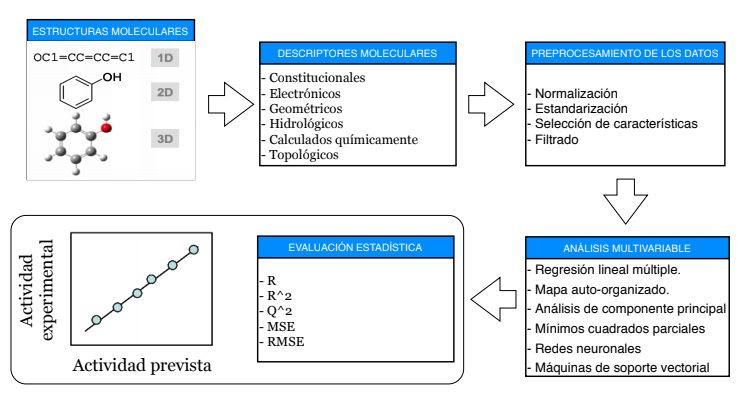
\includegraphics[scale=0.45]{Capitulo1/figuras/figura1.png}
    \caption{Pasos a seguir para realizar el modelado por QSAR.}
    \label{figura1}
\end{figure}
\noindent De la figura anterior se definen a los compuestos, de acuerdo con la Encyclopedia Britannica, como cualquier sustancia compuesta de moléculas idénticas que consisten en átomos de dos o más elementos químicos.\cite{8}\\

\noindent Para obtener la información de los compuestos y sus respectivas estructuras moleculares, se utiliza DrugBank. DrugBank es una base de datos en línea completa y de libre acceso que contiene información sobre fármacos. Como un recurso bioinformático y químico-informático, DrugBank combina datos detallados de medicamentos (es decir, químicos, farmacológicos y farmacéuticos) con información completa sobre el objetivo del medicamento (es decir, secuencia, estructura y vía).\\

\noindent Luego los descriptores moleculares pueden definirse como la información esencial de una molécula en términos de sus propiedades fisicoquímicas (constitución, electrónica, geométrica, etc) de acuerdo con el artículo\textit{ A PRACTICAL OVERVIEW OF QUANTITATIVE STRUCTURE - ACTIVITY RELATIONSHIP} de la revista en línea para las ciencias experimentales y clínicas (\textit{EXCLI}, por sus siglas en inglés)\cite{9}.\\

\noindent La información referente a los descriptores se obtiene utilizando PubChem. PubChem es una base de datos de moléculas químicas y sus actividades contra ensayos biológicos. El sistema es mantenido por el Centro Nacional de Información Biotecnológica (NCBI, por sus siglas en inglés), un componente de la Biblioteca Nacional de Medicina (NLM, por sus siglas en inglés), que forma parte de los Institutos Nacionales de Salud (NIH, por sus siglas en inglés) de los Estados Unidos.
En ese mismo artículo se habla sobre los módulos restantes de la figura \ref{figura1}, que se detallan a continuación.\\

\noindent En el apartado del preprocesamiento de los datos, cuando se obtiene la información sobre los compuestos y sus descriptores, se advierte que dicha información puede tener inconsistencias, por eso, para realizar un análisis preciso, se debe “limpiar” y dejar un conjunto de datos mejorado.\\

\noindent Luego, el módulo denominado análisis multivariante define esencialmente un enfoque para discernir cuantitativamente las relaciones entre las variables independientes (p. ej., descriptores moleculares) y las variables dependientes (p. ej., actividades biológicas de interés).\\

\noindent Ahora, para un modelo QSAR robusto es necesario validar el modelo así como aplicar parámetros estadísticos para evaluar su rendimiento predictivo. Esto se hace en el módulo de evaluación estadística.\\

\noindent Finalmente, como resultado de todos los módulos mencionados anteriormente, se obtiene la información acerca del comportamiento (por predicción) de un conjunto de datos (fármacos) frente a cierta patología (proteínas).\\

\noindent La metodología QSAR es interdisciplinaria, por lo que recibe información de la Química Orgánica y de la Farmacología. En concreto, QSAR persigue el diseño molecular dirigido de compuestos con potencial farmacológico, permitiendo el ahorro de recursos económicos y humanos.\\

\noindent Una de las ventajas más notables en el uso de QSAR es el hecho de que al ser una ciencia que existe sólo en un entorno virtual – desmaterializado de necesidades de infraestructura (tales como equipo, instrumentos, materiales y personal de laboratorio) – con enfoque en las relaciones estructura (química) – actividad (biológica), el diseño de candidatos a nuevos fármacos es mucho más económico y rápido. En cuanto a sus desventajas están la familiarización con metodologías computacionales (diferentes sistemas operativos e interfaces gráficas, manejo de bases de datos, desarrollo del software) y en este sentido, la resolución de diferentes problemas de cómputo (compatibilidad, actualizaciones, registros, formatos de datos) así como el hecho de tener que disponer de datos de actividad biológica de las moléculas que provengan de una misma fuente.\\

\subsubsection{\textit{Machine Learning}}
\noindent El término de \textit{Machine Learning}, hace referencia a lograr que una máquina aprenda sin programarlas explícitamente, para esto existen 4 métodos generales, los cuales son:\\

\noindent- Supervisado.\\
- No supervisado.\\
- Semi-supervisado.\\
- Refuerzo de aprendizaje.\\

\noindent Siendo así, los objetivos de \textit{Machine Learning} consisten en lograr que máquinas sean capaces de realizar predicciones, realizar agrupamiento de conjuntos, tomar decisiones a partir de un conjunto de datos, u obtener reglas de asociación.\cite{10}\\

\noindent \textit{Machine Learning} tiene un gran vínculo  con la optimización   muchos problemas de aprendizaje se formulan como la minimización de alguna función de pérdida en un conjunto de ejemplos de capacitación. Las funciones de pérdida expresan la discrepancia entre las predicciones del modelo que se está entrenando y las instancias del problema real (por ejemplo, en la clasificación, uno quiere asignar una etiqueta a las entradas, y los modelos están entrenados para predecir correctamente las etiquetas preasignadas de un conjunto de ejemplos).\\
\section{Métodos de \textit{Machine Learning}}
\subsection{Árbol de decisión de aprendizaje}
\noindent Un árbol tiene muchas analogías en la vida real, y resulta que ha influido en un área amplia del aprendizaje automático, cubriendo tanto la clasificación como la regresión. En el análisis de decisiones, se puede usar un árbol de decisiones para representar visual y explícitamente las decisiones y la toma de decisiones. Como su nombre indica, utiliza un modelo de decisiones en forma de árbol.
En resumen se dibuja un árbol de decisión al revés con su raíz en la parte superior. Se tiene una condición / nodo interno, en función del cual el árbol se divide en ramas/bordes. El final de la rama que ya no se divide es la decisión(hoja).\\

\noindent Sin embargo, un conjunto de datos real tendrá muchas más funciones y esto solo será una rama en un árbol mucho más grande, pero no puede ignorar la simplicidad de este algoritmo. La importancia de la característica es clara y las relaciones se pueden ver fácilmente. Esta metodología se conoce más comúnmente como árbol de decisión de aprendizaje de los datos y el árbol anterior se llama árbol de clasificación, ya que el objetivo es clasificar a los pasajeros como sobrevivientes o fallecidos. Los árboles de regresión se representan de la misma manera, solo predicen valores continuos como el precio de una casa. En general, los algoritmos del Árbol de decisión se denominan CART o Árboles de clasificación y regresión.\\
%%%%%%%%%%%%%%%%%%%%%%%%%%%%%%%%%%%%%%%%%%%%%%%%55
\subsection{Redes Neuronales Artificiales}
\noindent Un algoritmo de aprendizaje de la red neuronal artificial (RNA), generalmente llamado ``red neuronal'' (RN), es un algoritmo de aprendizaje inspirado en la estructura y los aspectos funcionales de las redes neuronales biológicas. Los cálculos se estructuran en términos de un grupo interconectado de neuronas artificiales, que procesan la información utilizando un enfoque conexionista para el cálculo\cite{11}. Las redes neuronales modernas son herramientas de modelado de datos estadísticos no lineales. Por lo general, se usan para modelar relaciones complejas entre entradas y salidas, para encontrar patrones en los datos o para capturar la estructura estadística en una distribución de probabilidad conjunta desconocida entre las variables observadas.
%%%%%%%%%%%%%%%%%%%%%%%%%%%%%%%%%%%%%%%%%%%%%%
\subsection{Máquina  de Soporte Vectorial (SVM)}
\noindent La Máquina de Soporte Vectorial es otro algoritmo simple que todo experto en aprendizaje automático debería tener en su arsenal. La máquina de vectores de soporte es muy preferida por muchos, ya que produce una precisión significativa con menos potencia de cálculo. Maquina de Soporte Vectorial, abreviado como SVM por sus siglas en inglés, se puede usar tanto para tareas de regresión como de clasificación. Pero, es ampliamente utilizado en los objetivos de clasificación. El objetivo del algoritmo de máquina de vectores de soporte es encontrar un hiperplano en un espacio N-dimensional (N - el número de características) que clasifica claramente los puntos de datos.\\

\noindent Para separar las dos clases de puntos de datos, hay muchos hiperplanos posibles que podrían elegirse. Nuestro objetivo es encontrar un plano que tenga el margen máximo, es decir, la distancia máxima entre los puntos de datos de ambas clases. Maximizar la distancia de margen proporciona cierto refuerzo para que los puntos de datos futuros se puedan clasificar con más confianza\cite{12}.\\
%%%%%%%%%%%%%%%%%%%%%%%%%%%%%%%%%%%%%%%%%%%%%%%%%%%%
\subsection{Aprendizaje por refuerzo}
\noindent El Aprendizaje por refuerzo se refiere a cómo un agente debe tomar medidas en un entorno para maximizar alguna noción de recompensa a largo plazo. Los algoritmos de aprendizaje por refuerzo intentan encontrar una política que asigne estados del mundo a las acciones que el agente debe tomar en esos estados. El aprendizaje de refuerzo difiere del problema de aprendizaje supervisado en que los pares de entrada / salida correctos nunca se presentan, ni las acciones subóptimas se corrigen explícitamente.\\

\noindent El aprendizaje de refuerzo, debido a su generalidad, se estudia en muchas otras disciplinas, como la teoría de juegos, la teoría de control, la investigación de operaciones, la teoría de la información, la optimización basada en simulación, los sistemas de múltiples agentes, la inteligencia de enjambre, las estadísticas y los algoritmos genéticos. En la literatura de investigación y control de operaciones, el aprendizaje por refuerzo se denomina programación dinámica aproximada o programación neurodinámica.\\

%%%%%%%%55
\section{\textit{Machine Learning} en la Bioinformática}
\noindent \textit{Machine Learning} se ha convertido en uno de los temas que más se ha desarrollado, siendo muy útil para el descubrimiento de nuevos fármacos asistidos por computadora, esto ya que \textit{Machine Learning} aprovecha el uso de algoritmos para la clasificación y reconocimientos de patrones, aprovecha estas bases para predecir propiedades físicas, químicas incluso biológicas de nuevos compuestos. Otra enorme ventaja es la gran eficiencia para la lectura y análisis de gran cantidad de datos sin requerir una vasta cantidad de recursos.  Hoy en día las técnicas de \textit{Machine Learning} pueden ser usadas para el modelado QSAR y así lograr el desarrollo de programas inteligentes con la capacidad de predecir por in-silico la forma en que modificaciones químicas pueden influir en el comportamiento biológico.\\

\noindent Gracias a esto actualmente hay gran cantidad de aplicaciones y estudios de la Bioinformática, pues la principal meta de estas técnicas es adquirir exitosamente información útil por medio de la elaboración de abstracción probabilística.  En general consiste en programas computacionales, para optimizar un proceso utilizando algún dato como ejemplo o experiencia previamente adquirida.\\

\noindent De acuerdo con un artículo del Diario de Química Medicinal recuperado por el Centro Nacional de Información Biotecnológica de los Estados Unidos, el aumento de las medidas para regular la producción y venta de productos químicos, así como la reducción de recursos para las pruebas de dichos productos, han hecho que los modelos de QSAR se utilicen cada vez más en la detección, la priorización de pruebas, las iniciativas de prevención de la contaminación, la química ecológica, la identificación de peligros y la evaluación de riesgos. Sin embargo, para ser aceptados por los usuarios finales (toxicólogos, reguladores, industria), estos QSAR deben cumplir con una gama de necesidades, incluida la relevancia para los esquemas regulatorios, la transparencia, la plausibilidad biológica y la comprensión por parte de los no desarrolladores.\\

\noindent La revista Future-Science, en el artículo Current trends in quantitative structure–activity relationship validation and applications on drug discovery, menciona que Las técnicas de \textit{Machine Learning} se han empleado ampliamente en el campo QSAR para construir modelos de regresión y clasificación utilizando grandes conjuntos de datos de dominio público y / o utilizando conjuntos grandes que contienen descriptores calculados

%%%%%%%%%%%%%%%%%%%%%%%%%%%%%%%%%%%%%%%%%%%%%5
\section{Alternativas de solución}
\noindent En la actualidad, los métodos de \textit{Machine Learning} y la metodología de QSAR permiten tener una visión más novedosa y menos egoísta hacia la experimentación, en la cual se haga uso de las ventajas que ofrece la tecnología para realizar este proceso involucrando el menor número de animales posible.
Es por ello que tanto \textit{Machine Learning} como QSAR pueden enfocarse al ámbito del diseño de fármacos asistido por computadora para construir un sistema que realice el proceso de la experimentación científica con mayor rapidez, obteniendo mejores resultados, y reduciendo el uso de seres vivos para dicho proceso.\\

\noindent De hecho, sistemas como el que se propuso anteriormente ya existen. Cabe destacar que debido a la cantidad de información que puede arrojar el análisis de grado molecular de una bacteria (sin mencionar virus, hongos, etc.), las soluciones actuales que se presentan, hacen uso el uso de métodos \textit{in silico} ó \textit{in vitro} y normalmente se enfocan a un área de la medicina en particular (cardiología, oftalmología, etc.)\\

\noindent Un ejemplo es el software Virtual Assay, desarrollado por la Universidad de Oxford, que provee un marco de trabajo para realizar pruebas in-silico en poblaciones de modelos de células cardíacas humanas para predicciones de seguridad y eficacia de fármacos.\\

\noindent Organs-on-chips diseñados por el Instituto Wyss de Harvard, en donde se han adaptado los métodos de fabricación de microchips de computadora para diseñar dispositivos de cultivo de microfluidos que recapitulan la microarquitectura y las funciones de los órganos humanos vivos.\\

\noindent Los modelos de tejido vendidos por MatTek, que son sistemas micro-fisiológicos de los tejidos epiteliales humanos en modelos 3D de tejidos vivos y metabólicamente activos que permiten a los investigadores la flexibilidad de los experimentos agudos o a largo plazo en un entorno altamente fisiológico e in vitro y que se basan en el concepto de sustituir las pruebas en animales.\\

\noindent En la tabla \ref{productos1} se detalla a cada uno de los ejemplos mencionados, incluyendo a la solución propuesta.
Además de estos ejemplos, existen otros más que si bien entran en la categoría de alternativas ya existentes al problema planteado, se encuentran aún en desarrollo, tienen un enfoque diferente al presentado en este documento o solo fueron trabajos meramente académicos.\\

\noindent Software como TOPKAT, enfocado a la toxicología, que explota la estructura molecular de un compuesto para medir y aprobar evaluaciones de sus efectos tóxicos y ambientales, o la aplicación VEGA, que ofrecer una familia de herramientas para evaluar el peligro químico de cierto compuesto son solo algunos de ellos. En la tabla \ref{productos2} se encuentra una lista completa con toda la información de estos y más ejemplos de software para el modelado .\cite{13}

\begin{longtable}{|c|l|c|}
\caption{Resumen de productos similares.}
\label{productos1}\\
\hline
SOFTWARE & \multicolumn{1}{c|}{CARACTER\'iSTICAS} & PRECIO EN EL MERCADO \\ \hline
\endfirsthead
%
\multicolumn{3}{c}%
{{\bfseries Tabla \thetable\ Continuación de la página anterior.}} \\
\hline

\endhead
%
\textit{Virtual Assay} & \begin{tabular}[c]{@{}l@{}}- Marco de trabajo para la\\   realizaci\'on de experimentos por\\   medio del modelado por\\   computadora.\\   - Enfocado a la cardiolog\'ia.\\   - Su m\'etodo de trabajo es el\\    ajuste de modelos   \\   celulares comparados con\\    experimentaciones previas.\end{tabular} & NO COMERCIAL \\ \hline
\textit{Organs-on-Chips} & \begin{tabular}[c]{@{}l@{}}- Se basa en el uso de c\'elulas\\    vivas, adaptadas en pequeños\\   chips.\\   - Permiten la observaci\'on de las\\   c\'elulas humanas y su reacci\'on\\    ante enfermedades espec\'ificas.\\   - Es un m\'etodo in-vitro,\\    no involucra el uso de un \\   software.\end{tabular} & \begin{tabular}[c]{@{}c@{}}\$2,495 USD por placa\\ (6 chips).\end{tabular} \\ \hline
\textit{\begin{tabular}[c]{@{}c@{}}Modelos de tejido \\ MatTek's\end{tabular}} & \begin{tabular}[c]{@{}l@{}} - Son modelos de tejido 3D\\    vivos y metab\'olicamente \\   activos.\\   - Es un m\'etodo in-vitro.\\   - Actualmente tiene modelos\\    para pruebas oculares,\\   dermatol\'ogicas, intestinales y\\   genitales.\end{tabular} & SIN INFORMACIÓN \\ \hline
\textit{Soluci\'on propuesta} & \begin{tabular}[c]{@{}l@{}}- Se basa en el modelado\\    matem\'atico de QSAR.\\   - Es un m\'etodo in-silico.\\   - Utiliza \textit{Machine Learning} \\   para asistir y complementar\\    los resultados de QSAR.\end{tabular} & N/A \\ \hline
\end{longtable}
\begin{longtable}{|c|l|c|}
\caption{Resumen de software académicos o con enfoque diferente al problema planteado.}
\label{productos2}\\

\hline
SOFTWARE & \multicolumn{1}{c|}{CARACTER\'iSTICAS} & PRECIO EN EL MERCADO \\ \hline
\endfirsthead
%
\multicolumn{3}{c}%
{{\bfseries Tabla \thetable\ Continuación de la página anterior.}} \\
\hline

\endhead
%
PASS & \begin{tabular}[c]{@{}l@{}}- Capaz de calcular m\'as\\  de 4000 tipos de\\ actividad biol\'ogica.\\ - Requiere la f\'ormula \\ estructural del\\ compuesto.\\ - Utiliza una base de \\ datos que contiene\\ 260,000 compuestos \\ aproximadamente.\\ - Es comercial.\end{tabular} & NO DISPONIBLE \\ \hline
\textit{TOPKAT} & \begin{tabular}[c]{@{}l@{}}- Enfoque a la toxicidad  de los\\ compuestos.\\ - Modelado utilizando \\ QSTR para el enfoque toxicol\'ogico.\end{tabular} & NO DISPONIBLE \\ \hline
\textit{VEGA hub} & \begin{tabular}[c]{@{}l@{}}- Conjunto de herramientas\\ , enfocadas a la\\ predicci\'on y an\'alisis de la \\ toxicidad de un compuesto.\\ - Una de las herramientas \\ utiliza QSAR para\\ realizar predicciones\end{tabular} & GRATUITO \\ \hline
\textit{Leadscope} & \begin{tabular}[c]{@{}l@{}}- Enfoque en el an\'alisis\\  de toxicidad en\\ una simulaci\'on de los\\  sistemas biol\'ogicos de\\  un roedor.\\ - Utiliza modelos para\\  reproducci\'on,\\ neurotoxicidad, problemas\\  gen\'eticos y agentes\\  cancer\'igenos.\end{tabular} & NO DISPONIBLE \\ \hline
\textit{Derek Nexus} & \begin{tabular}[c]{@{}l@{}}- Enfoque al an\'alisis\\  toxicol\'ogico.\\   - Utiliza su propia \\ base de datos (base\\   privada).\end{tabular} & NO COMERCIAL \\ \hline
ADMET predictor & \begin{tabular}[c]{@{}l@{}}- Se basa en redes\\  neuronales para realizar\\ predicciones ADMET\\  (Absorci\'on, Distribuci\'on,\\  Metabolismo, Eliminaci\'on\\  y Toxicidad) \\ de medicamentos.\\ - Es comercial.\\ - Requiere de un nivel\\  intermedio en habilidades\\  computacionales.\\ - Se enfoca en las \\ propiedades qu\'imicas\\  de los compuestos.\end{tabular} & NO DISPONIBLE \\ \hline
OSIRIS & \begin{tabular}[c]{@{}l@{}}- Realiza an\'alisis de las \\ propiedades\\ f\'isico-qu\'imicas de \\ una mol\'ecula.\\ - Indica beneficios y \\ desventajas acerca de\\ la mol\'ecula estudiada.\\ - La mol\'ecula debe ser \\ construida por el\\ usuario.\end{tabular} & GRATUITO \\ \hline
T.E.S.T. & \begin{tabular}[c]{@{}l@{}}- Utiliza varias metodolog\'ias\\  de QSAR para\\ predicciones toxicol\'ogicas.\\ - Trabaja con la estructura \\ de un compuesto, ya\\ sea en archivo, creado en su \\ herramienta o de una base de\\  datos espec\'ifica.\end{tabular} & GRATUITO \\ \hline
CASE & \begin{tabular}[c]{@{}l@{}}- Capaz de predecir efectos\\  toxicol\'ogicos\\ en animales.\\ - Utiliza el modelo de \\ regresi\'on lineal.\\ - Se encuentra en desarrollo.\end{tabular} & NO DISPONIBLE \\ \hline
LAZAR & \begin{tabular}[c]{@{}l@{}}- Uso de algoritmos\\  estad\'isticos\\  para predecirtoxicidad.\\ - Es un proyecto web.\end{tabular} & GRATUITO \\ \hline
\end{longtable}
\newpage
\section{Arquitectura del sistema}
\noindent Por lo cual, el sistema que se planea desarrollar utilizará la información fisicoquímica y las referencias de experimentaciones previas de un conjunto de fármacos, se realiza una predicción de la actividad biológica de dicho conjunto, utilizando técnicas de \textit{Machine Learning} y QSAR para obtener una medida cuantitativa que permita clasificarlos del más al menos recomendable.\\

\noindent El modelo del sistema está compuesta por tres bloques principales de los cuales podemos clasificar como entradas, proceso y salidas.\\

a)	Entradas.\\

\noindent Las entradas están dadas por una lista de compuestos y una lista de proteínas de la patología, como requerimiento, los nombres de los compuestos y de las proteínas, deberán estar escritas en el idioma ingles para tener una búsqueda eficaz. Con estas listas el sistema puede comenzar la búsqueda de lo siguientes datos: \\

\noindent 1.- Conjunto de compuestos: El sistema recibe datos de diversos compuestos candidatos dados por el usuario, estos interactúan con una proteína perteneciente a una patología, estos datos los obtendremos de la base de datos “DrugBank”.\\

\noindent 2.- Descriptores moleculares: El sistema hará la búsqueda de datos más específicos del conjunto de compuestos previamente mencionados, dichos descriptores poseen información de las propiedades fisicoquímicas, describiendo numéricamente a cada una de las moléculas, estos datos los localizamos en la base de datos “PubChem”.\\

\noindent 3.- Proteínas de la enfermedad: Esta entrada otorga al sistema la información del objeto de estudio, para determinar las actividades biológicas que provocará su interacción con cada uno de los componentes listados en la primera entrada, al igual que en los compuestos, esta información podrá ser localizada en las base de de datos “PDB”.\\

 b)	Procesos.\\
El sistema hará uso de la metodología de QSAR para modelar cada una de las entradas obtenidas y así poder describir numéricamente la molécula, con lo cual el sistema hará  uso de un algoritmo de \textit{Machine Learning} y así poder determinar el resultado de la interacción entre proteína y compuesto, además de que el sistema adquiere la experiencia de esa interacción, para una posible interacción con características similares.\\

c) 	Salidas.\\
Actividad biológica de los compuestos ingresados: El sistema otorgará información y descripción de la actividad biológica causada por el compuesto que haya interactuado con la proteína objetivo, para conocer cuál de los compuestos ingresados obtiene el mejor de los resultados, el sistema generará una lista con dichos resultados que será desplegada al usuario, ordenada del compuesto más apto al menos apto para enfrentar la patología indicada.
\begin{figure}[H]
    \centering
    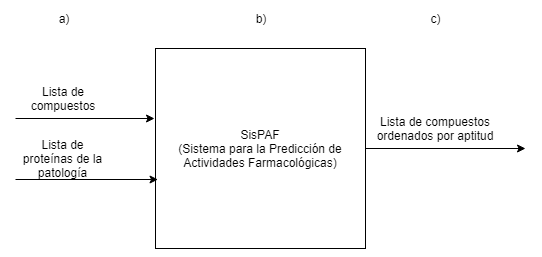
\includegraphics[scale=0.8]{Capitulo1/figuras/arquitectura.png}
    \caption{Arquitectura del sistema}
    \label{arq}
\end{figure}
 %Obligatorio
\lhead{Capítulo \ref{ch_2-1}}
\rhead{\newtitle}
\cfoot{\thepage}
\renewcommand{\headrulewidth}{1pt}
\renewcommand{\footrulewidth}{1pt}

\chapter{Planificación de Sistemas de Información}\label{ch_2-1}
%Planificación: la 3, la 5.
%Viabilidad: la 1, 2, 4, 6.
\noindent Se tiene como objetivo la obtención de un marco de referencia para el desarrollo del sistema de información que responda a los objetivos estratégicos planteados. Este marco de referencia consta de:\\

\begin{itemize}
    \item Una descripción de la situación actual, que constituirá el punto de partida del Plan de Sistemas de Información. Dicha descripción incluirá un análisis técnico de puntos fuertes y riesgos, así como el análisis de servicio a los objetivos de la organización.
    \item Un conjunto de modelos que constituya la arquitectura de información.
    \item Una propuesta de calendario para la ejecución de dichos proyectos.
    \item Un plan de seguimiento y cumplimiento de todo lo propuesto mediante unos mecanismos de evaluación adecuados.
\end{itemize}

\section{Estudio de la Información Relevante}{
\noindent Los animales son ampliamente utilizados en la experimentación científica para el desarrollo de medicinas y para probar la seguridad de otros productos. Dados los recientes avances en la Bioinformática, especialmente en el modelado in-silico (asistido por computadora) como lo es QSAR, y los algoritmos que realizan predicciones como los pertenecientes al área de \textit{Machine Learning}, el proceso de la experimentación tiene una visión diferente en cuanto a la forma en que se realiza.\\

\noindent QSAR es una metodología que reúne un conjunto de modelos computacionales relacionados con el diseño, la visualización espacial, la virtualización de moléculas y el cálculo de sus propiedades fisicoquímicas, mediante la Bioinformática y la Estadística. Todo esto con el objetivo de hacer una predicción de la actividad biológica referente a los compuestos seleccionados, que permita el diseño teórico de posibles nuevos fármacos, evitando pasar por el proceso de prueba y error de la síntesis orgánica.\\

\noindent Los modelos QSAR son ecuaciones matemáticas donde se relaciona la actividad biológica con descriptores moleculares o información fisicoquímica de una estructura química \cite{anex_1}. Para poder construir un modelo de QSAR debemos tomar en cuenta un número de moléculas con valores conocidos de actividad biológica.
Posteriormente, se calculan algunos descriptores moleculares en los que destacan los de tipo fisicoquímico, constitucional, geométrico, topológico y electrónico, estos se calculan a partir de una estructura virtual 3D por métodos computacionales, por lo que son un reflejo cuantitativo o describen numéricamente a cada una de las moléculas. Estos pueden ser de diferentes tipos, y ello depende de la complejidad de información que requiera el cálculo. El número de descriptores a considerar está en función de las herramientas computacionales de cálculo con que se cuente y del número de moléculas incluidas en el estudio, estos descriptores se usan como
variables independientes en la ecuación QSAR.\\

\subsection{\textit{Machine Learning}}

\noindent Por otra parte, \textit{Machine Learning} es un subcampo de las Ciencias de la computación que se enfoca al desarrollo de técnicas que permiten predecir comportamientos futuros mediante la recolección de datos y el diseño de algoritmos, por lo que es usado en gran cantidad de aplicaciones y estudios de la Bioinformática, pues la principal meta de estas técnicas es adquirir exitosamente información útil por medio de la elaboración de abstracción probabilística. En general consiste en programas computacionales, para optimizar un proceso utilizando algún dato como ejemplo o experiencia previamente adquirida.\\

\noindent El objetivo principal del \textit{Machine Learning} es crea un sistema que aprenda automáticamente. Aprender en este contexto quiere decir identificar patrones complejos en millones de datos. Lo que realmente aprende una máquina es un algoritmo que revisa los datos y es capaz de predecir comportamientos futuros.\\

\noindent Existen distintos algoritmos en el campo del \textit{Machine Learning}, en los cuales destaca la regresión lineal simple y regresión lineal múltiple, esto por ser pieza fundamental dentro de los demás algoritmos (Redes Neuronales, Maquina de soporte vectorial , etc).\\

\noindent La regresión lineal múltiple permite generar un modelo lineal en el que el valor de la variable dependiente o respuesta (Y) se determina a partir de un conjunto de variables independientes llamadas predictores (X1, X2, X3…). Es una extensión de la regresión lineal simple, por lo que es fundamental comprender esta última. Los modelos de regresión múltiple pueden emplearse para predecir el valor de la variable dependiente o para evaluar la influencia que tienen los predictores sobre ella (esto último se debe que analizar con cautela para no malinterpretar causa-efecto).

Los modelos lineales múltiples siguen la siguiente ecuación:

\begin{equation}
    Y_i = (\beta_0 + \beta_1 X_1i + \beta_2 X_2i + ... + \beta_n X_ni ) + e_i
\end{equation}

\begin{itemize}
   
 \item $\beta_0$: Es la ordenada en el origen, el valor de la variable dependiente Y cuando todos los predictores son cero.\\

\item $\beta_i$: Es el efecto promedio que tiene el incremento en una unidad de la variable predictora $X_i$ sobre la variable dependiente $Y$, manteniéndose constantes el resto de variables. Se conocen como coeficientes parciales de regresión.
\item $e_i$: Es el residuo o error, la diferencia entre el valor observado y el estimado por el modelo.
\end{itemize}

\noindent Es importante tener en cuenta que la magnitud de cada coeficiente parcial de regresión depende de las unidades en las que se mida la variable predictora a la que corresponde, por lo que su magnitud no está asociada con la importancia de cada predictor. Para poder determinar qué impacto tienen en el modelo cada una de las variables, se emplean los coeficientes parciales estandarizados, que se obtienen al estandarizar (sustraer la media y dividir entre la desviación estándar) las variables predictoras previo ajuste del modelo.

\subsubsection{Condiciones para la regresión lineal múltiple}
\noindent Los modelos de correlación lineal múltiple requieren de las mismas condiciones que los modelos lineales simples más otras adicionales.\\

\textit{No colinialidad o multicolinialidad}\\

\noindent En los modelos lineales múltiples los predictores deben ser independientes, no debe de haber colinialidad entre ellos. La colinialidad ocurre cuando un predictor está linealmente relacionado con uno o varios de los otros predictores del modelo o cuando es la combinación lineal de otros predictores. Como consecuencia de la colinialidad no se puede identificar de forma precisa el efecto individual que tiene cada una de las variables colineales sobre la variable respuesta, lo que se traduce en un incremento de la varianza de los coeficientes de regresión estimados hasta el punto que resulta prácticamente imposible establecer su significancia estadística.\\

\noindent No existe un método estadístico concreto para determinar la existencia de colinialidad o multicolinialidad entre los predictores de un modelo de regresión, sin embargo, se han desarrollado numerosas reglas prácticas que tratan de determinar en qué medida afecta a la estimación y contraste de un modelo. Los pasos recomendados a seguir son:

\begin{itemize}
    \item Si el coeficiente de determinación $\mathcal{R}^2$ es alto pero ninguno de los predictores resulta significativo, hay indicios de colinialidad.
    \item Calcular una matriz de correlación en la que se estudia la relación lineal entre cada par de predictores. Es importante tener en cuenta que, a pesar de no obtenerse ningún coeficiente de correlación alto, no está asegurado que no exista multicolinialidad. Se puede dar el caso de tener una relación lineal casi perfecta entre tres o más variables y que las correlaciones simples entre pares de estas mismas variables no sean mayores que 0.5.
    \item Generar un modelo de regresión lineal simple entre cada uno de los predictores frente al resto. Si en alguno de los modelos el coeficiente de determinación $\mathcal{R}^2$ es alto, estaría señalando a una posible colinialidad.
    \item Tolerancia (TOL) y Factor de Inflación de la Varianza (VIF). Se trata de dos parámetros que vienen a cuantificar lo mismo (uno es el inverso del otro). El VIF de cada predictor se calcula según la siguiente fórmula:
\end{itemize}

\begin{equation}
    VIF_(\hat{\beta}_j) = \frac{1}{1 - R^2}
\end{equation}

\begin{equation}
    Tolerancia_(\hat{\beta}_j) = \frac{1}{VIF_(\hat{\beta}_j)}
\end{equation}

Donde $\mathcal{R}^2$ se obtiene de la regresión del predictor $X_j$ sobre los otros predictores. Esta es la opción más recomendada, los límites de referencia que se suelen emplear son:

\begin{itemize}
    \item VIF = 1: Ausencia total de colinialidad
    \item 1 < VIF < 5: La regresión puede verse afectada por cierta colinialidad.
    \item 5 < VIF < 10: Causa de preocupación
    \item El termino tolerancia es 1/VIF por lo que los límites recomendables están entre 1 y 0.1.
\end{itemize}

\noindent En caso de encontrar colinialidad entre predictores, hay dos posibles soluciones. La primera es excluir uno de los predictores problemáticos intentando conservar el que, a juicio del investigador, está influyendo realmente en la variable respuesta. Esta medida no suele tener mucho impacto en el modelo en cuanto a su capacidad predictiva ya que, al existir colinialidad, la información que aporta uno de los predictores es redundante en presencia del otro. La segunda opción consiste en combinar las variables colineales en un único predictor, aunque con el riesgo de perder su interpretación.


\subsection{\textit{Docking}}{
\noindent El acoplamiento molecular es un método computacional utilizado para predecir la interacción de dos moléculas que generan un modelo de unión. En muchas aplicaciones de descubrimiento de fármacos, el acoplamiento se realiza entre una molécula pequeña y una macromolécula, por ejemplo, el acoplamiento de proteínas y ligandos. Más recientemente, el acoplamiento también se aplica para predecir el modo de unión entre dos macromoléculas, por ejemplo, el acoplamiento proteína-proteína.\\

\noindent Actualmente, la mecánica molecular es la base de la mayoría de los programas de acoplamiento. La mecánica molecular implica la descripción de un sistema poliatómico utilizando la física clásica. Los parámetros experimentales como las cargas, los ángulos de torsión y geométricos se utilizan para reducir la diferencia entre los datos experimentales y las predicciones de la mecánica molecular (Lopes, Guvench y Mackerell, 2015). Debido a las deficiencias y limitaciones de los parámetros experimentales, las ecuaciones matemáticas a menudo se pueden parametrizar sobre la base de cálculos semiempíricos y ab teóricos de mecánica cuántica. Como tal, los campos de fuerza molecular son conjuntos de ecuaciones con diferentes parámetros con el propósito final de describir los sistemas. Como los campos de fuerza pueden usar diferentes consideraciones y simplificaciones, la descripción del sistema puede ser inexacta debido al nivel de teoría involucrado (física clásica).\\

\noindent La mayoría de los campos de fuerza se basan en cinco términos, todos los cuales tienen una interpretación física: energía potencial, términos de torsión, geometría de enlace, términos electrostáticos y potencial de Lenard-Jones (Monticelli y Tieleman, 2013).\\

\noindent Con el uso de campos de fuerza, el modelado molecular y de proteínas se logró a principios de la década de 1980. Una extensión natural de estos métodos fue el modelado de procesos moleculares como la unión de proteínas y ligandos.\\
\noindent Se desarrollaron dos metodologías generales. Primero, el enfoque de cuerpo rígido que está estrechamente relacionado con el modelo clásico de Emil Fischer. En este modelo, el ligando y el receptor se consideran dos cuerpos independientes que se reconocen entre sí en función de la forma y el volumen.\\
\noindent El segundo enfoque es el acoplamiento flexible. Este enfoque considera un efecto recíproco del reconocimiento de proteínas y ligandos en la conformación de cada parte (Dastmalchi, 2016).

\subsection{Recomendaciones generales y pautas para el acoplamiento}

\subsubsection{Requisitos de hardware y software para acoplamiento molecular}

\noindent Antes de abordar los detalles científicos de la metodología de acoplamiento, comentaremos los requisitos generales de hardware para ejecutar el acoplamiento de manera eficiente. Por lo general, un cálculo de acoplamiento no se considera intensivo en CPU, ya que los ligandos se pueden acoplar y evaluar en un par de minutos. Actualmente, casi cualquier computadora personal (o computadora portátil) es lo suficientemente competente como para ejecutar una pequeña campaña de acoplamiento (alrededor de 500-1000 compuestos) en un tiempo razonable. Sin embargo, la detección virtual basada en el acoplamiento de repositorios públicos puede aumentar rápidamente (más de 106 compuestos), lo que requiere más recursos informáticos para terminar en un par de semanas. La Tabla II presenta las pautas generales recomendadas para una computadora antes de ejecutar el acoplamiento.\\


\subsubsection{Preparación de ligando y proteína}
\noindent El sistema debe seleccionarse y prepararse cuidadosamente antes de hacer cualquier cálculo. El primer paso es obtener una estructura de la proteína, preferiblemente con un ligando unido. ¿Qué estructura se debe usar? Se recomienda considerar estructuras tridimensionales con alta resolución o estructuras cristalizadas con ligandos de alta afinidad o sustratos naturales. Para algunas proteínas, esto puede no ser siempre el caso. En tales casos, se pueden utilizar estructuras con informes previos de atraque o estudios estructurales.\\

\noindent Como se mencionó anteriormente, el acoplamiento requiere la asignación de varios parámetros. La información contenida en un archivo del Protein Data Bank (PDB) a menudo es insuficiente y, por lo tanto, se requiere la rectificación de los archivos PDB. En la práctica, hay varios módulos de preparación disponibles (Tabla \ref{Tabla_Docking}), la mayoría de ellos pueden corregir problemas comunes en archivos PDB. Sin embargo, se ha demostrado que a menudo se pasan por alto algunos aspectos estructurales (Warren, Do, Kelley, Nicholls y Warren, 2012).

\begin{longtable}{|l|l|l|}
\caption{Software utilizado para la preparación de proteínas y ligandos.}
\label{Tabla_Docking}
\hline
\multicolumn{1}{|c|}{Software} & \multicolumn{1}{c|}{Tipo} & \multicolumn{1}{c|}{Características}                                                                                                                                                                                             \endfirsthead 
\hline
Autodock Tools                 & Académico                 & \begin{tabular}[c]{@{}l@{}}Limpieza de la estructura, asignación \\de carga (Gasteiger), selección del \\rotador y predicción del sitio de unión.\end{tabular}                                                                   \\ 
\hline
Openbabel                      & Código abierto            & \begin{tabular}[c]{@{}l@{}}Asignación de carga, múltiples formatos\\de archivo compatibles, conversión de archivos\end{tabular}                                                                                                  \\ 
\hline
MOE                            & Comercial                 & \begin{tabular}[c]{@{}l@{}}Corrección de problemas de residuos, \\limpieza de estructuras, asignación de \\carga basada en varios campos de fuerza, \\minimización de proteínas y predicción del sitio \\de unión.\end{tabular}  \\
\hline
\end{longtable}
}}
%%%%%%%%%%%%%%%%%%%%%%%%%%%%%%%%%%%%%%%%%%%%%%%%%%%
\section{Estudio de los Sistemas de Información Actuales}{
\noindent Las técnicas de \textit{Machine Learning} y la metodología de QSAR pueden enfocarse al ámbito de la Bioinformática para diseñar un sistema que realice el proceso de la experimentación científica con mayor rapidez, obteniendo mejores resultados, y reduciendo el uso de seres vivos para dicho proceso.\\

\noindent En la actualidad, este tipo de sistemas ya son una realidad. Un ejemplo es el software Virtual Assay, desarrollado por la Universidad de Oxford, que provee un marco de trabajo para realizar pruebas in-silico en poblaciones de modelos de células cardíacas humanas para predicciones de seguridad y eficacia de fármacos, bajo la justificación de que cada individuo responde de manera única a cierto fármaco, y que el proceso de la experimentación es costoso y poco eficaz.\\

\noindent Otros métodos utilizados como los Organs-on-chips diseñados por el Instituto Wyss de Harvard, que son esencialmente secciones transversales tridimensionales de unidades funcionales principales de órganos vivos completos, o los modelos de tejido vendidos por MatTek, que proporcionan una plataforma micro-fisiológica para modelar biología humana altamente relevante y predictiva. Ambas iniciativas, pertenecientes a la clasificación in-vitro (uso de células y tejido), junto con Virtual Assay, representan las opciones más relevantes para intentar cambiar la forma en la que se realiza el proceso de la experimentación clásica.\\

En la tabla \ref{productos1} se detalla a cada uno de los ejemplos mencionados, incluyendo a la solución propuesta.

\noindent Para el caso del \textit{Docking} existen en la actualidad sistemas y herramientas que fueron desarrolladas para ofrecer la automatización de este proceso, en la Tabla \ref{Herramienta_Dock} podemos observar estas herramientas.
Dichas herramientas nos ayudan a crear un proceso de acoplamiento molecular desde cero, algunas herramientas nos permiten realizar la preparación del ligando/proteína como el software AutoDock, podemos observar la Tabla \ref{Tabla_Docking} que nos muestra las herramientas que permiten realizar este procedimiento.

\begin{longtable}{|l|l|l|l|}
\caption{ Ejemplos de software disponible para el acoplamiento de proteínas y ligandos y su algoritmo de búsqueda}\\ 
\hline
\label{Herramienta_Dock}
\multicolumn{1}{|c|}{Nombre} & Algoritmo de búsqueda                                                                  & \multicolumn{1}{c|}{Tipo~} & \multicolumn{1}{c|}{Referencias}                                                          \endfirsthead 
\hline
AUTODOCK4                    & \begin{tabular}[c]{@{}l@{}}Algoritmo genético\\~\& lamarckiano, 2003\end{tabular}   & Académico                  & Morris et al., 2009                                                                       \\ 
\hline
HADDOCK                      & Híbrido                                                                                                     & Académico                  & \begin{tabular}[c]{@{}l@{}}Dominguez, Boelens\\~\& Bonvin, 2003\end{tabular}              \\ 
\hline
VINA                         & Optimización local                                                                                                                              & Académico                  & Trott  Olson, 2009                                                                        \\ 
\hline
LIGANDFIT                    & Coincidencia de forma                                                                                       & Comercial                  & \begin{tabular}[c]{@{}l@{}}Venkatachalam, Jiang,\\Oldfield \& Waldman, 2003\end{tabular}  \\ 
\hline
DOCK                         & Coincidencia de forma                                                                                      & Académico                  & Allen et al., 2015                                                                        \\ 
\hline
MOE                          & Híbrido                                                                                                     & Comercial                  & Vilar, Cozza  Moro, 2008                                                                  \\
\hline
\end{longtable}

}\newpage
%%%%%%%%%%%%%%%%%%%%%%%%%%%%%%%%%%%%%%%%%%%%%%%%%%
\section{Establecimiento del Alcance del Sistema}{
\noindent La experimentación, dentro de la industria farmacéutica, es una parte indispensable para el desarrollo de nuevos medicamentos que contribuyen a mejorar la salud humana. Por desgracia, este proceso implica el uso de animales como “sujetos de prueba”, poniendo en riesgo las vidas de otros seres vivos para hacer mejor la vida de los seres humanos. En la actualidad, los métodos de \textit{Machine Learning} y los modelos de QSAR permiten tener una visión más novedosa y menos egoísta hacia la experimentación, en la cual se haga uso de las ventajas que ofrece la tecnología para realizar este proceso involucrando el menor número de animales posible. Las capacidades del uso de la tecnología aplicadas al campo de la experimentación permitirían mejorar en gran medida dicha situación, tanto en costos, ya que no se tendría que gastar en la compra y mantenimiento de animales, como en ética, promoviendo una cultura en la que se respete el derecho a la vida para todo organismo.\\

\noindent Pro eso el objetivo principal es desarrollar un sistema basado en los modelos de QSAR (Quantitative Structure-Activity Relationship) y los métodos de Machine Learning usando el algoritmo de regresión lineal que permitirá simular el procedimiento de un experimento químico en un entorno computacional, el cual tendrá como resultado un conjunto de actividades biológicas que brinden información acerca de los beneficios o problemas de algún compuesto frente a ciertas proteínas, y representando una alternativa a la experimentación que involucra el uso de seres vivos.
}
%%%%%%%%%%%%%%%%%%%%%%%%%%%%%%%%%%%%%%%%%%%%%%%%%%
\newpage
\section{Estudio de la Situación Actual}{
\begin{longtable}{|c|l|c|}
\caption{Resumen de productos similares.}\\ 
\hline
SOFTWARE                                                                                 & \multicolumn{1}{c|}{CARACTERíSTICAS}                                                                                                                                                                                                                                                         & PRECIO EN EL MERCADO                                                        \endfirsthead 
\hline
\textit{Virtual Assay}                                                                   & \begin{tabular}[c]{@{}l@{}}- Marco de trabajo para la\\ realización de experimentos por\\ medio del modelado por\\ computadora.\\ - Enfocado a la cardiología.\\ - Su método de trabajo es el\\ ajuste de modelos \\ celulares comparados con\\ experimentaciones previas. \end{tabular}   & NO COMERCIAL                                                                \\ 
\hline
\textit{Organs-on-Chips}                                                                 & \begin{tabular}[c]{@{}l@{}}- Se basa en el uso de células\\ vivas, adaptadas en pequeños\\ chips.\\ - Permiten la observación de las\\ células humanas y su reacción\\ ante enfermedades específicas.\\ - Es un método in-vitro,\\ no involucra el uso de un \\ software. \end{tabular} & \begin{tabular}[c]{@{}c@{}}\$,495 USD por placa\\ (6 chips). \end{tabular}  \\ 
\hline
\begin{tabular}[c]{@{}c@{}}\textit{Modelos de tejido }\\\textit{ MatTek's} \end{tabular} & \begin{tabular}[c]{@{}l@{}} - Son modelos de tejido 3D\\ vivos y metabólicamente \\ activos.\\ - Es un método in-vitro.\\ - Actualmente tiene modelos\\ para pruebas oculares,\\ dermatológicas, intestinales y\\ genitales. \end{tabular}                                                 & SIN INFORMACIÓN                                                             \\ 
\hline
\textit{Solución propuesta}                                                             & \begin{tabular}[c]{@{}l@{}}- Se basa en el modelado\\ matemático de QSAR.\\ - Es un método in-silico.\\ - Utiliza \textit{Machine Learning} \\ para asistir y complementar\\ los resultados de QSAR. \end{tabular}                                                                          & N/A                                                                         \\
\hline
\end{longtable}
}
%%%%%%%%%%%%%%%%%%%%%%%%%%%%%%%%%%%%%%%%%%%%%%%%%%
\section{Selección de la Solución}{
\noindent Desarrollar un sistema informático basado en el modelo QSAR (Quantitative Structure-Activity Relationship) utilizando algoritmos de \textit{Machine Learning} (Regresión Lineal) que permitirá simular la experimentación química en un entorno computacional. El sistema tomara una serie de entradas (Lista compuestos y lista de proteínas) para obtener las estructuras moleculares de cada uno de ellos, de igual manera se tiene contemplado el uso de la actividad biológica y sus descriptores de cada compuesto.\\

\noindent Esta información sera procesada por nuestro sistema y a través del procedimiento de acoplamiento molecular (Docking) generar las variables necesarias para generar una regresión múltiple y poder predecir el comportamiento biológico de cada uno de los compuestos contra una proteína.\\

\noindent Estos resultados serán representados a través de una tabla que sera ordenada de mayor a menor 'efectividad' para adherirse y contrarrestar el funcionamiento de dicha proteína.\\
\noindent El sistema realizara un aprendizaje autónomo gracias al modelo que generara la regresión lineal múltiple por lo cual su eficiencia mejorara con cada iteración que se realice en el sistema. 
}
%%%%%%%%%%%%%%%%%%%%%%%%%%%%%%%%%%%%%%%%%%%%%%%%%%
\lhead{Capítulo \ref{ch_3}}
\rhead{\newtitle}
\cfoot{\thepage}
\renewcommand{\headrulewidth}{1pt}
\renewcommand{\footrulewidth}{1pt}

\chapter{Análisis del Sistema de Información}\label{ch_3}
\noindent La experimentación con animales es un recurso ampliamente utilizado por empresas que se dedican a la elaboración de fármacos, con el objetivo de garantizar que sus productos no dañan la salud humana. Este proceso somete a distintas especies a métodos de pruebas que, en su mayoría, les causan daños irreversibles. \\
En la actualidad, la presencia de la tecnología en el área de las ciencias médico-biológicas ha cambiado por completo la trayectoria para el desarrollo de los fármacos, identificando y descubriendo nuevas soluciones potenciales con una reducción significativa de costos y tiempo.
\newpage
%%%%%%%%%%%%%%%%%%%%%%%%%%%%%%%%%%%5%%%%%%%%%%%
\section{Estudio de Factibilidad}
\subsection{Factibilidad técnica}
\noindent En las tablas \ref{Est_Hard} y \ref{Est_Soft} se en listan los elementos de desarrollo que hacen posible la construcción del sistema.\\

- Hardware
% Please add the following required packages to your document preamble:
% \usepackage{longtable}
% Note: It may be necessary to compile the document several times to get a multi-page table to line up properly
\begin{longtable}{|l|l|c|}
\caption{Elementos de hardware disponibles para el desarrollo del sistema}
\label{Est_Hard}\\
\hline
\textbf{EQUIPO} & \textbf{DESCRIPCIÓN}                                                                                                                         & \multicolumn{1}{l|}{\textbf{CANTIDAD}} \\ \hline
\endfirsthead
%
\multicolumn{3}{c}%
{{\bfseries Tabla \thetable\ Continuación de la página anterior}} \\
\endhead
%
Computador      & \begin{tabular}[c]{@{}l@{}}Modelo: HP 15-ac128la\\ Procesador: Intel Core i7-6500U 2.50 GHz\\ RAM: 8 GB\\ Disco duro: 2 TB\end{tabular}      & 1                                      \\ \hline
Computador      & \begin{tabular}[c]{@{}l@{}}Modelo: HP Pavilion 15-cw1092lm\\ Procesador: AMD Ryzen 3 2300U \\ RAM: 12 GB\\ Disco duro: 1 TB\end{tabular}     & 1                                      \\ \hline
Computador      & \begin{tabular}[c]{@{}l@{}}Modelo: TOSHIBA MQ01ABD100\\ Procesador: Intel Core i7-6498DU 2.50GHz\\ RAM: 4 GB\\ Disco duro: 1 TB\end{tabular} & 1                                      \\ \hline
\end{longtable}

\noindent Computador HP 15-ac128la: Este computador se utilizará para desarrollar el sistema.\\
Computador HP Pavilion 15-cw1092lm: Este computador tendrá las tareas de desarrollo y pruebas del sistema.\\
Computador TOSHIBA MQ01ABD100: Este computador se utilizará para desarrollar el sistema.\\

- Software: Todos los computadores mencionados anteriormente tiene los mismos elementos de software.\\
% Please add the following required packages to your document preamble:
% \usepackage{longtable}
% Note: It may be necessary to compile the document several times to get a multi-page table to line up properly
\begin{longtable}{|l|l|l|}
\caption{Elementos de software disponibles para el desarrollo del sistema}
\label{Est_Soft}\\
\hline
\textbf{NOMBRE}    & \textbf{VERSIÓN}                                                                                                     & \textbf{DESCRIPCIÓN}                                                                                                                                    \\ \hline
\endfirsthead
%
\multicolumn{3}{c}%
{{\bfseries Tabla \thetable\ Continuación de la página anterior}} \\
\endhead
%
Linux              & \begin{tabular}[c]{@{}l@{}}Cualquier distribución en \\ su última versión estable.\\ (Basada en Debian)\end{tabular} & \begin{tabular}[c]{@{}l@{}}1GNU/Linux  es un sistema \\ operativo libre tipo Unix \\ POSIX; multiplataforma, \\ multiusuario y multitarea.\end{tabular} \\ \hline
Visual Studio Code & 1.38.0 o última versión estable.                                                                                     & \begin{tabular}[c]{@{}l@{}}Editor de texto enfocado \\ a la creación de código fuente.\end{tabular}                                                     \\ \hline
Python             & 3.7.4 o última versión estable.                                                                                      & \begin{tabular}[c]{@{}l@{}}Lenguaje de programación \\ de alto nivel multipropósito.\end{tabular}                                                       \\ \hline
Git                & 2.23.0 o última versión estable.                                                                                     & Sistema de control de versiones.                                                                                                                        \\ \hline
\end{longtable}
\noindent - Sistema operativo: Se considera el uso del sistema operativo [TAL] para las tareas de diseño, desarrollo y pruebas del sistema ya que ofrece mejores interfaces, es menos restrictivo y permite mayor comodidad a los desarrolladores en cuanto al cumplimiento de las tareas mencionadas previamente.\\

\noindent - Editor de texto: Este editor tiene como objetivo facilitar el proceso de creación de código, haciéndolo más cómodo y comprensible para los desarrolladores.\\

\noindent - Python: Python es un lenguaje de programación interpretado, de alto nivel y de propósito general. Creado por Guido van Rossum y lanzado por primera vez en 1991, la filosofía de diseño de Python enfatiza la legibilidad del código con su uso notable de espacios en blanco significativos.\\

\noindent - Git: Git es un sistema distribuido de control de versiones para rastrear cambios en el código fuente durante el desarrollo de software. Está diseñado para coordinar el trabajo entre programadores, pero se puede usar para rastrear cambios en cualquier conjunto de archivos.\\

\subsection{Factibilidad económica}
- Costos de software:\\
A continuación se presenta una descripción de los costos operativos necesarios para ejecutar los procedimientos del sistema propuesto, lo cual permite apreciar de mejor manera las bondades del mismo.\\
% Please add the following required packages to your document preamble:
% \usepackage{longtable}
% Note: It may be necessary to compile the document several times to get a multi-page table to line up properly
\begin{longtable}{|l|l|l|}
\caption{Costos por software}
\label{Costos_por_Software}\\
\hline
\textbf{NOMBRE}    & \textbf{CANTIDAD} & \textbf{COSTO} \\ \hline
\endfirsthead
%
\multicolumn{3}{c}%
{{\bfseries Tabla \thetable\ Continuación de la página anterior}} \\
\endhead
%
Linux              & 3                 & \$0.00         \\ \hline
Visual Studio Code & 3                 & \$0.00         \\ \hline
Python             & 3                 & \$0.00         \\ \hline
Git                & 2                 & \$0.00         \\ \hline
\multicolumn{2}{|l|}{TOTAL}            & \$0.00               \\ \hline
\end{longtable}
El costo de software para el sistema propuesto es nulo, pues se basa en la adquisición y uso de programas de software libre, que pueden ser obtenidos desde la web sin costo alguno.\\

- Costos de hardware:
La siguiente tabla muestra la depreciación de cada uno de los elementos de hardware que deberán comprarse para soportar la aplicación.\\
% Please add the following required packages to your document preamble:
% \usepackage{longtable}
% Note: It may be necessary to compile the document several times to get a multi-page table to line up properly
\begin{longtable}{|l|l|l|}
\caption{Costos por hardware}
\label{Costos_por_Hardware}\\
\hline
\textbf{NOMBRE}                     & \textbf{CANTIDAD} & \textbf{COSTO} \\ \hline
\endfirsthead
%
\multicolumn{3}{c}%
{{\bfseries Tabla \thetable\ Continuación de la página anterior}} \\
\endhead
%
Computador HP 15-ac128la            & 1                 & \$0.00         \\ \hline
Computador  HP Pavilion 15-cw1092lm & 1                 & \$0.00         \\ \hline
Computador TOSHIBA MQ01ABD100       & 1                 & \$0.00         \\ \hline
\multicolumn{2}{|l|}{TOTAL}                             & \$0.00         \\ \hline
\end{longtable}

Una vez más, puesto que los computadores previamente especificados no generan depreciación en el sentido de si son capaces o no de brindar soporte a la aplicación, el costo vuelve a ser nulo.\\

- Costos de mano de obra:
En la siguiente tabla se agrega de manera meramente informativa, la proposición de la mano de obra requerida para realizar este proyecto y los respectivos sueldos por las horas trabajadas.
% Please add the following required packages to your document preamble:
% \usepackage{longtable}
% Note: It may be necessary to compile the document several times to get a multi-page table to line up properly
\begin{longtable}{|l|l|l|l|}
\caption{Costos por mano de obra}
\label{Costos_por_mano_de_obra}\\
\hline
\textbf{NOMBRE}              & \textbf{CANTIDAD} & \textbf{TIEMPO} & \textbf{\begin{tabular}[c]{@{}l@{}}COSTO EN EL\\ MERCADO\end{tabular}} \\ \hline
\endfirsthead
%
\multicolumn{4}{c}%
{{\bfseries Tabla \thetable\ Continuación de la página anterior}} \\
\endhead
%
Project Manager              & 1                 & 12 meses        & \$15,000.00                                                            \\ \hline
Tester                       & 1                 & 12 meses        & \$17,000.00                                                            \\ \hline
Desarrollador Front-End y UI & 1                 & 12 meses        & \$15,000.00                                                            \\ \hline
Desarrollador Back-End       & 3                 & 12 meses        & \$20,000.00                                                            \\ \hline
TOTAL                        &                   &                 & \$107,000.00                                                           \\ \hline
\end{longtable}
Finalmente, la tabla \ref{Costos_por_mano_de_obra} indica el costo total del sistema propuesto.
% Please add the following required packages to your document preamble:
% \usepackage{longtable}
% Note: It may be necessary to compile the document several times to get a multi-page table to line up properly
\begin{longtable}{|l|c|}
\caption{Costos generados}
\label{Costos_generados}\\
\hline
\textbf{DESCRIPCIÓN} & \multicolumn{1}{l|}{\textbf{COSTO TOTAL}} \\ \hline
\endfirsthead
%
\multicolumn{2}{c}%
{{\bfseries Tabla \thetable\ Continuación de la página anterior}} \\
\endhead
%
Costos software      & \$0.00                                    \\ \hline
Costos hardware      & \$0.00                                    \\ \hline
TOTAL                & \$0.00                                    \\ \hline
\end{longtable}
Como se puede observar, el sistema no genera ningún costo.

\section{Factibilidad Operativa}
Esta parte del estudio se basó en la recolección de datos mediante encuestas realizadas al público objetivo del sistema que se desea desarrollar.
Los resultados arrojan que el sistema es factible operacionalmente, pues la mayoría de las personas encuestadas están de acuerdo con la solución que plantea el sistema al uso de los seres vivos en la experimentación.\\

- Encuesta.
Esta encuesta estuvo dirigida al personal que labora como profesor y a los alumnos de la carrera de Químico Farmacéutico Industrial de la Escuela Nacional de Ciencias Biológicas.\\

\noindent ¿Considera que el proceso para desarrollar nuevos fármacos, es eficiente?\\

\noindent ¿Piensa que las ciencias de la computación podrían ayudar a mejorar o cambiar por completo el proceso para desarrollar nuevos fármacos?\\

\noindent ¿Considera que el trato a los animales en la experimentación es justificable con el fin de mantener la salud de los seres humanos?\\

\noindent ¿Estaría de acuerdo en automatizar el proceso de la experimentación para el desarrollo de nuevos fármacos?\\

\noindent ¿Consideraría viable la construcción de un sistema que predice la efectividad de un fármaco frente a cierta patología?\\

\noindent ¿Cuál de las siguientes palabras cree que describen mejor a un sistema que predice la efectividad de los fármacos?\\
% Please add the following required packages to your document preamble:
% \usepackage{longtable}
% Note: It may be necessary to compile the document several times to get a multi-page table to line up properly
\begin{longtable}{|l|c|}
\caption{Resultados de encuesta}
\label{Resul_encu}\\
\hline
Posibles respuestas & \multicolumn{1}{l|}{Resultados} \\ \hline
\endfirsthead
%
\multicolumn{2}{c}%
{{\bfseries Tabla \thetable\ Continuación de la página anterior}} \\
\endhead
%
Rápido              & 3                               \\ \hline
Intuitivo           & 2                               \\ \hline
Preciso             & 15                              \\ \hline
Ordenado            & 10                              \\ \hline
Fácil de utilizar   & 12                              \\ \hline
Económico           & 8                               \\ \hline
Seguro              & 10                              \\ \hline
\end{longtable}



%%%%%%%%%%%%%%%%%%%%%%%%%%%%%%%%%%%%%%%%%
\section{Ámbito del sistema}
\noindent SisPAF (Sistema para la predicción de actividades farmacológicas) será una aplicación que permitirá realizar pruebas de aptitud para un conjunto de fármacos contra una patología particular, ambos definidos por el usuario.
SisPAF realizará pruebas en tiempo real para determinar qué fármacos son más aptos para combatir la patología indicada, generando una lista de resultados que indique las probabilidades de éxito que tiene cada fármaco de eliminar o controlar a la patología. 
Este sistema no sustituye el proceso de la experimentación en animales, sino que propone una alternativa para reducir la cantidad de seres vivos que se requieren para este proceso, al compactar los fármacos que desean probarse y ordenarlos del más recomendable al menos recomendable.
%%%%%%%%%%%%%%%%%%%%%%%%%%%%%%%%%%%%%%%%%%%
\section{Establecimiento de Requisitos}
\subsection{Obtención de Requisitos}
%Requerimientos funcionales
% Please add the following required packages to your document preamble:
% \usepackage{longtable}
% Note: It may be necessary to compile the document several times to get a multi-page table to line up properly
\begin{longtable}{|l|l|l|l|l|l|}
\caption{Requerimientos funcionales}
\label{RF}\\
\hline
No & Concepto & Requerimiento & N\textbackslash{}D & Descripción & Naturaleza \\ \hline
\endfirsthead
%
\multicolumn{5}{c}%
{{\bfseries Tabla \thetable\ Continuación de la página anterior}} \\
\endhead
%
1 & Función & \begin{tabular}[c]{@{}l@{}}Búsqueda de\\  información\end{tabular} & Necesidad & \begin{tabular}[c]{@{}l@{}}La búsqueda de\\ información\\ referente a los\\ fármacos, sus\\ propiedades y \\ la patología\\ especificadas, \\ se realiza \\ utilizando las \\ bases de datos\\ especializadas\\ en compuestos,\\ descriptores\\ moleculares,\\ tablas de\\ propiedades\\ físico-químicas \\ y bancos de\\ proteínas.\end{tabular} & Cualitativa \\ \hline
1.1 & Función & \begin{tabular}[c]{@{}l@{}}Obtención y\\ lectura del\\ archivo base\end{tabular} & Necesidad & \begin{tabular}[c]{@{}l@{}}El sistema\\ recibe del\\ usuario un\\ archivo de\\ texto plano en\\ el cual se tiene\\ una lista con\\ los nombres\\ de los\\ compuestos y\\ nombres de\\ las proteínas\\ de la patología\\ que forman\\ parte del\\ objeto de\\ estudio.\end{tabular} & Cualitativa \\ \hline
1.2 & Función & \begin{tabular}[c]{@{}l@{}}Búsqueda\\ de los\\ compuestos\\ indicados.\end{tabular} & Necesidad & \begin{tabular}[c]{@{}l@{}}Por cada\\ elemento de la\\ lista de\\ compuestos en\\ el archivo\\ ingresado por\\ el usuario, el\\ sistema los\\ buscará en la\\ base de datos\\ en línea\\ “DrugBank”.\end{tabular} & Cualitativa \\ \hline
1.3 & Función & \begin{tabular}[c]{@{}l@{}}Búsqueda de\\ los\\ descriptores\\ de los\\ compuestos.\end{tabular} & Necesidad & \begin{tabular}[c]{@{}l@{}}El sistema,\\ utilizando\\ como\\ referencia la\\ lista de\\ compuestos\\ ingresada por\\ el usuario,\\ realiza una\\ búsqueda de los\\ \\ descriptores\\ físico químicos\\ por cada uno\\ de los elementos\\ de dicha lista en\\ las bases de\\ datos\\ “PubChem” y\\ “ChemSpider”.\end{tabular} & Cualitativa \\ \hline
1.4 & Función & \begin{tabular}[c]{@{}l@{}}Búsqueda de\\ los\\ mecanismos de\\ acción de los\\ compuestos.\end{tabular} & Necesidad & \begin{tabular}[c]{@{}l@{}}El sistema,\\ utilizando\\ como\\ referencia la\\ lista de\\ compuestos\\ ingresada por\\ el usuario,\\ realiza la\\ búsqueda de\\ las actividades\\ biológicas por\\ cada uno de\\ los elementos\\ de dicha lista\\ en la base de\\ datos\\ “DrugBank”.\end{tabular} & Cualitativa \\ \hline
1.5 & Función & \begin{tabular}[c]{@{}l@{}}Búsqueda de\\ las proteínas\\ indicadas.\end{tabular} & Necesidad & \begin{tabular}[c]{@{}l@{}}Por cada\\ elemento de la\\ lista de\\ proteínas en el\\ archivo\\ ingresado por\\ el usuario, el\\ sistema las\\ buscará en la\\ base de datos\\ en línea\\ “PDB”.\end{tabular} & Cualitativa \\ \hline
1.6 & Función & \begin{tabular}[c]{@{}l@{}}Confirmación\\ de los\\ resultados de\\ la búsqueda.\end{tabular} & Necesidad & \begin{tabular}[c]{@{}l@{}}El sistema\\ presenta al\\ usuario los\\ resultados de\\ la búsqueda y\\ este último\\ valida que\\ sean\\ correctos.\end{tabular} & Cualitativa \\ \hline
1.7 & Función & \begin{tabular}[c]{@{}l@{}}Construcción\\ de conjuntos.\end{tabular} & Necesidad & \begin{tabular}[c]{@{}l@{}}El sistema\\ organiza la\\ información\\ recabada\\ durante el\\ proceso de\\ búsqueda, en\\ archivos con\\ estructuras\\ definidas,\\ denominados\\ conjuntos, que\\ permiten\\ continuar a la\\ fase de\\ procesamiento\\ de\\ información.\end{tabular} & Cualitativa \\ \hline
1.7.1 & Función & \begin{tabular}[c]{@{}l@{}}Construcción\\ del conjunto\\ cero.\end{tabular} & Necesidad & \begin{tabular}[c]{@{}l@{}}El sistema\\ agrupa los\\ datos de los\\ compuestos en\\ un archivo\\ denominado\\ conjunto cero.\end{tabular} & Cualitativa \\ \hline
1.7.2 & Función & \begin{tabular}[c]{@{}l@{}}Construcción\\ del conjunto P\end{tabular} & Necesidad & \begin{tabular}[c]{@{}l@{}}El sistema\\ agrupa la\\ información de\\ la(s)\\ proteína(s)\\ (nombre de la\\ proteína,\\ estructura\\ molecular de la\\ proteína) de la\\ patología\\ indicada por el\\ usuario, en un\\ archivo\\ denominado\\ conjunto P.\end{tabular} & Cualitativa \\ \hline
2 & Función & \begin{tabular}[c]{@{}l@{}}Procesamiento \\ y obtención de\\ resultados.\end{tabular} & Necesidad & \begin{tabular}[c]{@{}l@{}}El sistema\\ obtiene los\\ datos tanto de \\ los compuestos\\ como de la(s)\\ proteína(s) a\\ partir de su \\ conjunto de\\ información\\ correspondientes.\end{tabular} & Cualitativa \\ \hline
2.1 & Función & \begin{tabular}[c]{@{}l@{}}Adquisición y \\ descomposición\\  del conjunto 0.\end{tabular} & Necesidad & \begin{tabular}[c]{@{}l@{}}El sistema lee el\\ conjunto 0\\ (previamente\\ definido)\\ correspondiente\\ a un compuesto,\\ para\\ descomponerlo y \\ obtener nombre,\\ descriptores ,\\ estructura\\ molecular y\\ actividad\\ biológica.\end{tabular} & Cualitativa \\ \hline
2.2 & Función & \begin{tabular}[c]{@{}l@{}}Adquisición y\\ descomposición\\ del conjunto P.\end{tabular} & Necesidad & \begin{tabular}[c]{@{}l@{}}El sistema\\ consigue el\\ nombre de la\\ proteína de\\ interés así como\\ su estructura\\ molecular esta\\ información\\ proveniente del\\ conjunto P.\end{tabular} & Cualitativa \\ \hline
2.3 & Función & \begin{tabular}[c]{@{}l@{}}Método de\\ Machine\\ Learning para\\ optimización.\end{tabular} & Necesidad & \begin{tabular}[c]{@{}l@{}}El sistema,   a\\ través de este\\ módulo trabaja \\ con los datos\\ correspondientes\\ al compuesto  y\\ proteína con el\\ objetivo de\\ optimizar la\\ obtención de\\ resultados.\end{tabular} & Cualitativa \\ \hline
2.4 & Función & \begin{tabular}[c]{@{}l@{}}Modelado \\ QSAR.\end{tabular} & Necesidad & \begin{tabular}[c]{@{}l@{}}El sistema\\ producirá con los\\ datos\\ pertenecientes a\\ la proteína y \\ compuesto de\\ interés  el\\ modelo QSAR\\ propio de la\\ actividad\\ farmacológica\\ entre el fármaco\\ y la proteína\\ objetivo.\end{tabular} & Cualitativa \\ \hline
3 & Función & \begin{tabular}[c]{@{}l@{}}Administración\\ y presentación\\ de resultados-\end{tabular} & Necesidad & \begin{tabular}[c]{@{}l@{}}El sistema recibe\\ el conjunto final\\ que está\\ constituido del\\ nombre del\\ compuesto y su\\ aptitud, datos\\ necesarios para\\ ordenar y\\ mostrar los\\ resultados.\end{tabular} & Cualitativa \\ \hline
3.1 & Función & \begin{tabular}[c]{@{}l@{}}Lectura y\\ ordenamiento\\ del conjunto\\ final.\end{tabular} & Necesidad & \begin{tabular}[c]{@{}l@{}}El sistema recibe\\ el conjunto final\\ que contiene el\\ nombre del\\ compuesto y la \\ aptitud, dicha\\ información será\\ leída y ordena\\ del más apto al\\ menos apto para\\ enfrentar la\\ proteína de la \\ patología\\ indicada. A la\\ salida se tiene\\ un archivo de\\ texto plano que\\ contiene una\\ lista ordenada.\end{tabular} & Cualitativa \\ \hline
3.2 & Función & \begin{tabular}[c]{@{}l@{}}Diseño gráfico\\ de resultados.\end{tabular} & Necesidad & \begin{tabular}[c]{@{}l@{}}El sistema\\ obtiene el\\ archivo que\\ contiene la lista\\ ordenada  la cual\\ será utilizada\\ para desplegar\\ de manera\\ gráfica  al\\ usuario.\end{tabular} & Cualitativa \\ \hline
\end{longtable}
\newpage
%Requerimientos No funcionales
% Please add the following required packages to your document preamble:
% \usepackage{longtable}
% Note: It may be necessary to compile the document several times to get a multi-page table to line up properly
\begin{longtable}{|l|l|l|l|l|l|}
\caption{Requerimientos no funcionales.}
\label{RNF}\\
\hline
No & Concepto & Requerimiento & N\textbackslash{}D & Descripción & Prioridad \\ \hline
\endhead
%
% 1 & Eficiencia & \begin{tabular}[c]{@{}l@{}}Tiempo de\\ respuesta.\end{tabular} & Necesidad & \begin{tabular}[c]{@{}l@{}}El sistema debe\\ realizar el\\ procesamiento de\\ los datos dentro de\\ un tiempo\\ establecido.\end{tabular} & 5 \\ \hline
1 & Eficacia & \begin{tabular}[c]{@{}l@{}}Uso de\\ recursos.\end{tabular} & Necesidad & \begin{tabular}[c]{@{}l@{}}El procesamiento\\ del sistema debe\\ realizarse de\\ manera que cumpla\\ con el objetivo\\ establecido\\ utilizando la mínima\\ cantidad de\\ recursos\\ necesarios.\end{tabular} & 5 \\ \hline
2 & Usabilidad & \begin{tabular}[c]{@{}l@{}}Interfaz con \\ Claridad\end{tabular} & Deseo & \begin{tabular}[c]{@{}l@{}}El sistema debe\\ cumplir con lo\\ establecido en la\\ norma ISO 13407\\ para que se\\ considere que la\\ interfaz es intuitiva\\ y amigable.\end{tabular} & 4 \\ \hline
3 & Almacenamiento & \begin{tabular}[c]{@{}l@{}}Opción de\\ respaldo de\\ resultados\end{tabular} & Deseo & \begin{tabular}[c]{@{}l@{}}Al obtener los\\ resultados, el\\ sistema dará la\\ opción al usuario\\ de almacenarlos o\\ desecharlos.\end{tabular} & 5 \\ \hline
\end{longtable}
\newpage
\subsection{Análisis de Requisitos}
%Descripcion de los requerimientos funcionales
% Please add the following required packages to your document preamble:
% \usepackage{longtable}
% Note: It may be necessary to compile the document several times to get a multi-page table to line up properly
\begin{longtable}{|l|l|}
\caption{Requerimiento funcional 1}
\label{RF1}\\
\hline
\begin{tabular}[c]{@{}l@{}}Nombre del requerimiento funcional:\\ Búsqueda de información de las variables\\  de entrada del sistema\end{tabular}                                                                                   & ID: RF1                                                                               \\ \hline
\endfirsthead
%
\multicolumn{2}{c}%
{{\bfseries Tabla \thetable\ Continuación de la página anterior}} \\
\endhead
%
\multicolumn{2}{|l|}{Área: Búsqueda de información.}                                                                                                                                                                                                                                                                       \\ \hline
\multicolumn{2}{|l|}{Actor(es): Usuario del sistema.}                                                                                                                                                                                                                                                                      \\ \hline
\multicolumn{2}{|l|}{Interesados: Sistema.}                                                                                                                                                                                                                                                                                \\ \hline
\multicolumn{2}{|l|}{\begin{tabular}[c]{@{}l@{}}Descripción: Obtener información de los datos ingresados por el usuario \\ mediante la lectura de un archivo y la búsqueda de su contenido en las bases de\\ datos en línea correspondientes.\end{tabular}}                                                             \\ \hline
\multicolumn{2}{|l|}{Evento desencadenador:}                                                                                                                                                                                                                                                                               \\ \hline
\multicolumn{2}{|l|}{Tipo de desencadenador: Externo y temporal.}                                                                                                                                                                                                                                                          \\ \hline
Pasos realizados (ruta principal)                                                                                                                                                                                                  & Información para los pasos                                                            \\ \hline
\begin{tabular}[c]{@{}l@{}}1.- El usuario inicia el programa esperando\\ que este termine de cargar su interfaz.\end{tabular}                                                                                                      & \begin{tabular}[c]{@{}l@{}}No se requiere información para\\  este paso.\end{tabular} \\ \hline
\begin{tabular}[c]{@{}l@{}}2.- El usuario ingresa un archivo de texto \\ plano reconocido por el sistema como \\ “archivo base” y da clic en el botón “buscar”.\end{tabular}                                                       & \begin{tabular}[c]{@{}l@{}}Archivo que se desea cargar al \\ sistema.\end{tabular}    \\ \hline
\begin{tabular}[c]{@{}l@{}}3.-  El sistema lee el archivo y procede a\\ buscar la información de cada elemento \\ contenido en dicho archivo.\end{tabular}                                                                         & \begin{tabular}[c]{@{}l@{}}No se requiere información para\\ este paso.\end{tabular}  \\ \hline
\begin{tabular}[c]{@{}l@{}}4.- El sistema almacena la información \\ obtenida y al finalizar su búsqueda presenta la \\ información al usuario con la finalidad de que \\ este observe los resultados de la búsqueda.\end{tabular} & \begin{tabular}[c]{@{}l@{}}No se requiere información para\\ este paso.\end{tabular}  \\ \hline
\multicolumn{2}{|l|}{Extensiones o Rutas alternativas.}                                                                                                                                                                                                                                                                    \\ \hline
\multicolumn{1}{|c|}{N/A}                                                                                                                                                                                                            & \multicolumn{1}{c|}{N/A}                                                                \\ \hline
\multicolumn{2}{|l|}{\begin{tabular}[c]{@{}l@{}}Precondiciones: El usuario ingresa un archivo de texto plano, el archivo cumple \\ con la estructura indicada por el sistema para su correcta lectura.\end{tabular}}                                                                                                       \\ \hline
\multicolumn{2}{|l|}{\begin{tabular}[c]{@{}l@{}}Postcondiciones: El usuario puede observar los datos que el sistema ha \\ obtenido y verificar que son correctos.\end{tabular}}                                                                                                                                            \\ \hline
\multicolumn{2}{|l|}{\begin{tabular}[c]{@{}l@{}}Suposiciones: El usuario tiene una buena conexión a internet, el programa \\ instalado y el dato especificado existe en las bases de datos.\end{tabular}}                                                                                                                  \\ \hline
\multicolumn{2}{|l|}{\begin{tabular}[c]{@{}l@{}}Garantía de éxito: El usuario puede obtener y seleccionar el dato que coincida en\\ la mayor exactitud con el que él desea.\end{tabular}}                                                                                                                                  \\ \hline
\multicolumn{2}{|l|}{Garantía mínima: El usuario ingresa datos reales que comprueba el sistema.}                                                                                                                                                                                                                           \\ \hline
\multicolumn{2}{|l|}{\begin{tabular}[c]{@{}l@{}}Requerimientos cumplidos: Búsqueda de información sobre las variables de\\ entrada del sistema.\end{tabular}}                                                                                                                                                              \\ \hline
\multicolumn{2}{|l|}{Prioridad: Alta.}                                                                                                                                                                                                                                                                                     \\ \hline
\multicolumn{2}{|l|}{Riesgo: Alto.}                                                                                                                                                                                                                                                                                        \\ \hline
\end{longtable}
% Please add the following required packages to your document preamble:
% \usepackage{longtable}
% Note: It may be necessary to compile the document several times to get a multi-page table to line up properly
\begin{longtable}{|l|l|}
\caption{Requerimiento funcional 1.1}
\label{RF11}\\
\hline
\begin{tabular}[c]{@{}l@{}}Nombre del requerimiento funcional:\\ Adquisición del archivo base.\end{tabular}                                                                                                                                                                               & ID: RF1.1                                                                                                                                     \\ \hline
\endfirsthead
%
\multicolumn{2}{c}%
{{\bfseries Tabla \thetable\ Continuación de la página anterior}} \\
\endhead
%
\multicolumn{2}{|l|}{Área: Búsqueda de información.}                                                                                                                                                                                                                                                                                                                                                                                      \\ \hline
\multicolumn{2}{|l|}{Actor(es): Usuario del sistema.}                                                                                                                                                                                                                                                                                                                                                                                     \\ \hline
\multicolumn{2}{|l|}{Interesados: Sistema.}                                                                                                                                                                                                                                                                                                                                                                                               \\ \hline
\multicolumn{2}{|l|}{Descripción: Permitir al usuario cargar un archivo de texto plano a la aplicación.}                                                                                                                                                                                                                                                                                                                                  \\ \hline
\multicolumn{2}{|l|}{\begin{tabular}[c]{@{}l@{}}Evento desencadenador: El usuario, ya estando en la pantalla inicial del sistema,\\ da clic en el botón que contiene un icono de suma “+” para proceder a cargar\\ un archivo. \end{tabular}}                                                                                                                                                                                                                                                                                                                               \\ \hline
\multicolumn{2}{|l|}{Tipo de desencadenador: Externo.}                                                                                                                                                                                                                                                                                                                                                                                    \\ \hline
Pasos realizados (ruta principal)                                                                                                                                                                                                                                                         & Información para los pasos                                                                                                                    \\ \hline
\begin{tabular}[c]{@{}l@{}}1.- El usuario presiona el botón para cargar un\\ archivo al sistema.\end{tabular}                                                                                                                                                                             & \begin{tabular}[c]{@{}l@{}}No se requiere información para\\  este paso.\end{tabular}                                                         \\ \hline
\begin{tabular}[c]{@{}l@{}}2.- El sistema abre una ventana con los\\ directorios del ordenador donde se encuentra\\ el usuario, para que este último proceda a la\\ búsqueda del archivo que desea cargar.\end{tabular}                                                                   & \begin{tabular}[c]{@{}l@{}}No se requiere información para\\  este paso.\end{tabular}                                                         \\ \hline
\begin{tabular}[c]{@{}l@{}}3.- El usuario selecciona el archivo que desea\\ cargar (el sistema por defecto solo admite el\\ formato de texto plano para el archivo que va\\ a recibir), y presiona el botón “Abrir”.\end{tabular}                                                         & \begin{tabular}[c]{@{}l@{}}Archivo que se desea cargar al \\ sistema.\end{tabular}                                                                             \\ \hline
\multicolumn{2}{|l|}{\begin{tabular}[c]{@{}l@{}}4.- El usuario hace clic en el botón “Buscar”\\ para proceder a la lectura del archivo\\ ingresado.\end{tabular}}                                                                                                                                             &  \begin{tabular}[c]{@{}l@{}}No se requiere información para\\ este paso.\end{tabular}                                                                                 \\ \hline
\multicolumn{2}{|l|}{Extensiones o Rutas alternativas.}                                                                                                                                                                                                                                                                                                                                                                                   \\ \hline
\multicolumn{1}{|c|}{N/A}                                                                                                                                                                                                                                                                   & \multicolumn{1}{c|}{N/A}                                                                                                                        \\ \hline
\multicolumn{2}{|l|}{\begin{tabular}[c]{@{}l@{}}Precondiciones: El usuario ingresa un archivo de texto plano, el archivo cumple\\ con la estructura indicada para el archivo base (el cual se encuentra\\ definido en el diccionario de datos con el ID: AB) para su correcta lectura.\end{tabular}}                                                                                                                                                                                    \\ \hline
\multicolumn{2}{|l|}{\begin{tabular}[c]{@{}l@{}}Postcondiciones: El sistema ha podido leer y registrar los datos en el archivo\\ ingresado por el usuario.\end{tabular}}                                                                                                                                                                                                                                                                  \\ \hline
\multicolumn{2}{|l|}{\begin{tabular}[c]{@{}l@{}}Suposiciones: El sistema puede recibir y leer archivos de texto plano, el archivo\\ ingresado por el usuario es válido tanto en formato como en estructura. Si el\\ archivo no es de texto plano, o no cumple con la estructura que solicita el sistema,\\ no se procederá con la ejecución de la aplicación y se notificará al usuario de que\\ el archivo no pudo leerse.\end{tabular}} \\ \hline
\multicolumn{2}{|l|}{\begin{tabular}[c]{@{}l@{}}Garantía de éxito: El sistema obtiene la información necesaria para el modelado\\ QSAR utilizando como referencia la información contenida en el archivo que el\\ usuario ingresó.\end{tabular}}                                                                                                                                                                                          \\ \hline
\multicolumn{2}{|l|}{Garantía mínima: No hay garantía mínima.}                                                                                                                                                                                                                                                                                                                                                                            \\ \hline
\multicolumn{2}{|l|}{Requerimientos cumplidos: Adquisición del archivo base.}                                                                                                                                                                                                                                                                                                                                                             \\ \hline
\multicolumn{2}{|l|}{Prioridad: Alta.}                                                                                                                                                                                                                                                                                                                                                                                                    \\ \hline
\multicolumn{2}{|l|}{Riesgo: Medio.}                                                                                                                                                                                                                                                                                                                                                                                                      \\ \hline
\end{longtable}
% Please add the following required packages to your document preamble:
% \usepackage{longtable}
% Note: It may be necessary to compile the document several times to get a multi-page table to line up properly
\begin{longtable}{|l|l|}
\caption{Requerimiento funcional 1.2}
\label{RF1_2}\\
\hline
\begin{tabular}[c]{@{}l@{}}Nombre del requerimiento funcional:\\ Búsqueda de los compuestos indicados.\end{tabular}                                                                                   & ID: RF1.2                                                                                                \\ \hline
\endfirsthead
%
\multicolumn{2}{c}%
{{\bfseries Tabla \thetable\ Continuación de la página anterior}} \\
\endhead
%
\multicolumn{2}{|l|}{Área: Búsqueda de información.}                                                                                                                                                                                                                                                             \\ \hline
\multicolumn{2}{|l|}{Actor(es): Usuario del sistema.}                                                                                                                                                                                                                                                            \\ \hline
\multicolumn{2}{|l|}{Interesados: Sistema.}                                                                                                                                                                                                                                                                      \\ \hline
\multicolumn{2}{|l|}{\begin{tabular}[c]{@{}l@{}}Descripción: Buscar si el nombre de cada compuesto en la lista dada por el\\ usuario existe en la base de datos “DrugBank” para obtener su estructura\\ molecular en un archivo con formato pdb..\end{tabular}}                                                  \\ \hline
\multicolumn{2}{|l|}{\begin{tabular}[c]{@{}l@{}}Evento desencadenador: Luego de que el sistema haya realizado la lectura del \\archivo base ingresado por el usuario, inmediatamente se procederá a realizar la \\búsqueda de los compuestos que se indican en el archivo mencionado anteriormente.\end{tabular}}                                                                                                                                                                                                                                                                     \\ \hline
\multicolumn{2}{|l|}{Tipo de desencadenador: Externo.}                                                                                                                                                                                                                                                           \\ \hline
Pasos realizados (ruta principal)                                                                                                                                                                     & Información para los pasos                                                                               \\ \hline
\begin{tabular}[c]{@{}l@{}}1.- El sistema lee el archivo ingresado,\\ busca la etiqueta “Compounds:” y \\obtiene una lista de compuestos.\end{tabular}                                                & Archivo cargado al sistema.                                                                              \\ \hline
\begin{tabular}[c]{@{}l@{}}2.-  El sistema se conecta a la base de\\ datos en línea “DrugBank”.\end{tabular}                                                                                          & \begin{tabular}[c]{@{}l@{}}No se requiere información para\\  este paso.\end{tabular}                    \\ \hline
\begin{tabular}[c]{@{}l@{}}3.- El sistema realiza la consulta\\ correspondiente a los nombres para cada\\ uno de los compuestos y obtiene su\\ estructura molecular.\end{tabular}                     & Lista de nombres de compuestos.                                                                          \\ \hline
\begin{tabular}[c]{@{}l@{}}4.- El sistema obtiene un archivo con \\extensión pdb para cada compuesto \\validado y lo almacena en el ordenador.\end{tabular}                           & \begin{tabular}[c]{@{}l@{}}No se requiere información para\\ este paso.\end{tabular}                     \\ \hline
\multicolumn{2}{|l|}{Extensiones o Rutas alternativas.}                                                                                                                                                                                                                                                          \\ \hline
\multicolumn{1}{|c|}{N/A}                                                                                                                                                                               & \multicolumn{1}{c|}{N/A}                                                                                   \\ \hline
\multicolumn{2}{|l|}{Precondiciones: El sistema ya ha validado y leído el archivo base.}                                                                                                                                                                                                                         \\ \hline
\multicolumn{2}{|l|}{\begin{tabular}[c]{@{}l@{}}Postcondiciones: El sistema valida la existencia de los compuestos dados por el\\ usuario en la base de datos “DrugBank”, obtiene sus estructuras moleculares en\\ archivos con extensión “pdb”, y puede continuar con su búsqueda de información.\end{tabular}} \\ \hline
\multicolumn{2}{|l|}{\begin{tabular}[c]{@{}l@{}}Suposiciones: El usuario ha ingresado correctamente el nombre de cada\\ compuesto, el archivo base se ha leído correctamente y la base de datos\\ “DrugBank” se encuentra accesible.\end{tabular}}                                                               \\ \hline
\multicolumn{2}{|l|}{\begin{tabular}[c]{@{}l@{}}Garantía de éxito: El sistema confirma que los compuestos dados por el usuario\\ existen, almacena la estructura molecular de cada compuesto, y se permite\\ proceder a obtener el resto de la información de cada compuesto.\end{tabular}}                      \\ \hline
\multicolumn{2}{|l|}{\begin{tabular}[c]{@{}l@{}}Garantía mínima: El sistema realiza la búsqueda sobre la base de datos\\ “Drugbank” y almacena las estructuras moleculares de los compuestos\\ encontrados.\end{tabular}}                                                                                        \\ \hline
\multicolumn{2}{|l|}{Requerimientos cumplidos: Búsqueda de los compuestos indicados.}                                                                                                                                                                                                                            \\ \hline
\multicolumn{2}{|l|}{Prioridad: Alta.}                                                                                                                                                                                                                                                                           \\ \hline
\multicolumn{2}{|l|}{Riesgo: Medio.}                                                                                                                                                                                                                                                                             \\ \hline
\end{longtable}
% Please add the following required packages to your document preamble:
% \usepackage{longtable}
% Note: It may be necessary to compile the document several times to get a multi-page table to line up properly
\begin{longtable}{|l|l|}
\caption{Requerimiento funcional 1.3}
\label{RF1_3}\\
\hline
\begin{tabular}[c]{@{}l@{}}Nombre del requerimiento funcional:\\ Búsqueda de los descriptores de los compuestos.\end{tabular}                                                                                                                                                                                                               & ID: RF1.3                                                                                                                      \\ \hline
\endfirsthead
%
\multicolumn{2}{c}%
{{\bfseries Tabla \thetable\ Continuación de la página anterior}} \\
\endhead
%
\multicolumn{2}{|l|}{Área: Búsqueda de información.}                                                                                                                                                                                                                                                                                                                                                                                                                         \\ \hline
\multicolumn{2}{|l|}{Actor(es): Sistema.}                                                                                                                                                                                                                                                                                                                                                                                                                                    \\ \hline
\multicolumn{2}{|l|}{Interesados: Sistema, usuario del sistema.}                                                                                                                                                                                                                                                                                                                                                                                                             \\ \hline
\multicolumn{2}{|l|}{\begin{tabular}[c]{@{}l@{}}Descripción: Utilizar las bases de datos “ChemSpider” y “PubMed” para recopilar\\ toda la información posible acerca de las propiedades fisicoquímicas de cada\\ compuesto validado por el sistema.\end{tabular}}                                                                                                                                                                                                            \\ \hline
\multicolumn{2}{|l|}{\begin{tabular}[c]{@{}l@{}}Evento desencadenador: Luego de que el sistema haya realizado la búsqueda\\ para identificar los compuestos ingresados por el usuario, inmediatamente se\\ procederá a realizar la búsqueda de los descriptores para los compuestos de los\\ que el sistema tenga confirmada su existencia.\end{tabular}}                                                                                                                    \\ \hline
\multicolumn{2}{|l|}{Tipo de desencadenador: Temporal.}                                                                                                                                                                                                                                                                                                                                                                                                                      \\ \hline
Pasos realizados (ruta principal)                                                                                                                                                                                                                                                                                                           & Información para los pasos                                                                                                     \\ \hline
\begin{tabular}[c]{@{}l@{}}1.- El sistema se conecta a las bases de datos\\ “ChemSpider” y “PubChem”.\end{tabular}                                                                                                                                                                                                                          & \begin{tabular}[c]{@{}l@{}}No se requiere información\\ para este paso.\end{tabular}                                           \\ \hline
\begin{tabular}[c]{@{}l@{}}2.-  El sistema realiza la consulta correspondiente\\ a los descriptores para cada uno de los\\ compuestos.\end{tabular}                                                                                                                                                                                         & \begin{tabular}[c]{@{}l@{}}Lista de nombres de\\ compuestos.\end{tabular}                                                      \\ \hline
\begin{tabular}[c]{@{}l@{}}3.- El sistema crea un archivo de texto plano\\ (temporal) donde en la primera línea indica el\\ nombre del compuesto al cual pertenece la\\ información ahí descrita, para luego copiar los\\ resultados obtenidos de la consulta realizada en\\ el paso anterior a dicho archivo.\end{tabular} & \begin{tabular}[c]{@{}l@{}}Nombre del compuesto al que\\ pertenece la información de\\ los descriptores obtenida.\end{tabular} \\ \hline
\multicolumn{2}{|l|}{Extensiones o Rutas alternativas.}                                                                                                                                                                                                                                                                                                                                                                                                                      \\ \hline
\multicolumn{1}{|c|}{N/A}                                                                                                                                                                                                                                                                                                                     & \multicolumn{1}{c|}{N/A}                                                                                                         \\ \hline
\multicolumn{2}{|l|}{\begin{tabular}[c]{@{}l@{}}Precondiciones: El sistema posee una lista de compuestos de los cuales ya ha\\ verificado su existencia.\end{tabular}}                                                                                                                                                                                                                                                                                                       \\ \hline
\multicolumn{2}{|l|}{\begin{tabular}[c]{@{}l@{}}Postcondiciones: El sistema obtiene la información de los descriptores de los\\ compuestos, necesaria para el proceso del modelado QSAR.\end{tabular}}                                                                                                                                                                                                                                                                       \\ \hline
\multicolumn{2}{|l|}{\begin{tabular}[c]{@{}l@{}}Suposiciones: El sistema ya ha verificado los compuestos de los cuales desea\\ obtener sus descriptores y las bases de datos “PubChem”, “ChemSpider” se\\ encuentran accesibles.\end{tabular}}                                                                                                                                                                                                                               \\ \hline
\multicolumn{2}{|l|}{\begin{tabular}[c]{@{}l@{}}Garantía de éxito: El sistema recopila la información proporcionada por los\\ descriptores fisicoquímicos de cada uno de los compuestos de la lista dada por el\\ usuario.\end{tabular}}                                                                                                                                                                                                                                     \\ \hline
\multicolumn{2}{|l|}{\begin{tabular}[c]{@{}l@{}}Garantía mínima: El sistema realiza la búsqueda sobre las base de datos\\ “PubChem” y “ChemSpider, y almacena los descriptores fisicoquímicos de los\\ compuestos encontrados.\end{tabular}}                                                                                                                                                                                                                                 \\ \hline
\multicolumn{2}{|l|}{Requerimientos cumplidos: Búsqueda de los descriptores de los compuestos.}                                                                                                                                                                                                                                                                                                                                                                              \\ \hline
\multicolumn{2}{|l|}{Prioridad: Alta.}                                                                                                                                                                                                                                                                                                                                                                                                                                       \\ \hline
\multicolumn{2}{|l|}{Riesgo: Alta}                                                                                                                                                                                                                                                                                                                                                                                                                                           \\ \hline
\end{longtable}
% Please add the following required packages to your document preamble:
% \usepackage{longtable}
% Note: It may be necessary to compile the document several times to get a multi-page table to line up properly
\begin{longtable}{|l|l|}
\caption{Requerimiento funcional 1.4}
\label{RF1_4}\\
\hline
\begin{tabular}[c]{@{}l@{}}Nombre del requerimiento funcional:\\ Búsqueda de los mecanismos de acción de los\\ compuestos.\end{tabular}                                                                                                                                                             & ID: RF1.4                                                                            \\ \hline
\endfirsthead
%
\multicolumn{2}{c}%
{{\bfseries Tabla \thetable\ Continuación de la página anterior}} \\
\endhead
%
\multicolumn{2}{|l|}{Área: Búsqueda de información.}                                                                                                                                                                                                                                                                                                                                         \\ \hline
\multicolumn{2}{|l|}{Actor(es): Sistema.}                                                                                                                                                                                                                                                                                                                                                    \\ \hline
\multicolumn{2}{|l|}{Interesados: Sistema, usuario del sistema.}                                                                                                                                                                                                                                                                                                                             \\ \hline
\multicolumn{2}{|l|}{\begin{tabular}[c]{@{}l@{}}Descripción: Obtener, utilizando la base de datos “DrugBank”, toda la\\ información posible acerca de las actividades biológicas de los compuestos\\ validados por el sistema.\end{tabular}}                                                                                                                                                 \\ \hline
\multicolumn{2}{|l|}{\begin{tabular}[c]{@{}l@{}}Evento desencadenador: Luego de que el sistema haya realizado la búsqueda\\ para identificar los compuestos ingresados por el usuario, inmediatamente se\\ procederá a realizar la búsqueda de las actividades biológicas para los\\ compuestos de los que el sistema tenga confirmada su existencia.\end{tabular}}                          \\ \hline
\multicolumn{2}{|l|}{Tipo de desencadenador: Temporal.}                                                                                                                                                                                                                                                                                                                                      \\ \hline
Pasos realizados (ruta principal)                                                                                                                                                                                                                                                                     & Información para los pasos                                                           \\ \hline
\begin{tabular}[c]{@{}l@{}}1.- El sistema se conecta a la base de datos\\ “Drugbank”.\end{tabular}                                                                                                                                                                                                    & \begin{tabular}[c]{@{}l@{}}No se requiere información\\ para este paso.\end{tabular} \\ \hline
\begin{tabular}[c]{@{}l@{}}2.- El sistema realiza la consulta\\ correspondiente a las actividades biológicas\\ para cada compuesto.\end{tabular}                                                                                                                                                      & Nombre del compuesto.                                                                \\ \hline
\begin{tabular}[c]{@{}l@{}}3.- Se almacena toda la información obtenida\\ en un archivo de texto plano temporal\\ denominado “MechOfAct”, donde se le agrega\\ una línea de texto indicando el nombre del\\ compuesto al que pertenece la información de\\ las actividades biológicas.\end{tabular} & \begin{tabular}[c]{@{}l@{}}No se requiere información para\\ este paso.\end{tabular} \\ \hline
\multicolumn{2}{|l|}{Extensiones o Rutas alternativas.}                                                                                                                                                                                                                                                                                                                                      \\ \hline
\multicolumn{1}{|c|}{N/A}                                                                                                                                                                                                                                                                               & \multicolumn{1}{c|}{N/A}                                                               \\ \hline
\multicolumn{2}{|l|}{\begin{tabular}[c]{@{}l@{}}Precondiciones: El sistema posee una lista de compuestos de los cuales ya ha\\ verificado su existencia.\end{tabular}}                                                                                                                                                                                                                       \\ \hline
\multicolumn{2}{|l|}{\begin{tabular}[c]{@{}l@{}}Postcondiciones: El sistema obtiene la información de las actividades biológicas\\ de los compuestos, necesaria para el proceso del modelado QSAR.\end{tabular}}                                                                                                                                                                             \\ \hline
\multicolumn{2}{|l|}{\begin{tabular}[c]{@{}l@{}}Suposiciones: El sistema ya ha verificado los compuestos de los cuales desea\\ obtener sus actividades biológicas y las base de datos “DrugBank” se encuentra\\ accesible.\end{tabular}}                                                                                                                                                     \\ \hline
\multicolumn{2}{|l|}{\begin{tabular}[c]{@{}l@{}}Garantía de éxito: El sistema recopila la información proporcionada por las\\ actividades biológicas de cada uno de los compuestos de la lista dada por el\\ usuario.\end{tabular}}                                                                                                                                                          \\ \hline
\multicolumn{2}{|l|}{\begin{tabular}[c]{@{}l@{}}Garantía mínima: El sistema realiza la búsqueda sobre la base de datos\\ “DrugBank” y almacena las actividades biológicas de los compuestos\\ encontrados.\end{tabular}}                                                                                                                                                                     \\ \hline
\multicolumn{2}{|l|}{\begin{tabular}[c]{@{}l@{}}Requerimientos cumplidos: Búsqueda de las actividades biológicas de los\\ compuestos.\end{tabular}}                                                                                                                                                                                                                                          \\ \hline
\multicolumn{2}{|l|}{Prioridad: Alta.}                                                                                                                                                                                                                                                                                                                                                       \\ \hline
\multicolumn{2}{|l|}{Riesgo: Alta}                                                                                                                                                                                                                                                                                                                                                           \\ \hline
\end{longtable}
% Please add the following required packages to your document preamble:
% \usepackage{longtable}
% Note: It may be necessary to compile the document several times to get a multi-page table to line up properly
\begin{longtable}{|l|l|}
\caption{Requerimiento funcional 1.5}
\label{RF1_5}\\
\hline
\begin{tabular}[c]{@{}l@{}}Nombre del requerimiento funcional:\\ Búsqueda de las proteínas indicadas.\end{tabular}                                                                           & ID: RF1.5                                                                                       \\ \hline
\endfirsthead
%
\multicolumn{2}{c}%
{{\bfseries Tabla \thetable\ Continuación de la página anterior}} \\
\endhead
%
\multicolumn{2}{|l|}{Área: Búsqueda de información.}                                                                                                                                                                                                                                           \\ \hline
\multicolumn{2}{|l|}{Actor(es): Usuario del sistema.}                                                                                                                                                                                                                                          \\ \hline
\multicolumn{2}{|l|}{Interesados: Sistema,}                                                                                                                                                                                                                                                    \\ \hline
\multicolumn{2}{|l|}{\begin{tabular}[c]{@{}l@{}}Descripción: Buscar si las proteínas indicadas por el usuario existen sobre la\\ base de datos “PDB”, de donde se obtendrá su estructura molecular.\end{tabular}}                                                                              \\ \hline
\multicolumn{2}{|l|}{\begin{tabular}[c]{@{}l@{}}Evento desencadenador: Luego de que el sistema obtenga las actividades\\ biológicas de los compuestos validados por el sistema, procederá\\ inmediatamente a buscar las proteínas indicadas por el usuario en el archivo\\ base.\end{tabular}} \\ \hline
\multicolumn{2}{|l|}{Tipo de desencadenador: Temporal.}                                                                                                                                                                                                                                        \\ \hline
Pasos realizados (ruta principal)                                                                                                                                                            & Información para los pasos                                                                      \\ \hline
\begin{tabular}[c]{@{}l@{}}1.- El sistema lee el archivo ingresado, busca\\ la etiqueta “Proteins:” y obtiene una lista de\\ proteínas.\end{tabular}                                         & Archivo cargado al sistema.                                                                     \\ \hline
\begin{tabular}[c]{@{}l@{}}2.- El sistema se conecta a la base de datos\\ “PDB”.\end{tabular}                                                                                                & \begin{tabular}[c]{@{}l@{}}No se requiere información para\\ este paso.\end{tabular}            \\ \hline
\begin{tabular}[c]{@{}l@{}}3.- El sistema realiza la consulta\\ correspondiente a los nombres para cada una\\ de las proteínas y obtiene su estructura\\ molecular.\end{tabular}             & Lista de nombres de proteínas                                                                   \\ \hline
\begin{tabular}[c]{@{}l@{}}4.- Por defecto, se obtendrá un archivo en\\ formato “pdb”, el cual se copiará a un\\ directorio temporal denominado “Proteins”.\end{tabular}                     & \begin{tabular}[c]{@{}l@{}}No se requiere información para\\ este paso.\end{tabular}            \\ \hline
\multicolumn{2}{|l|}{Extensiones o Rutas alternativas.}                                                                                                                                                                                                                                        \\ \hline
\multicolumn{1}{|c|}{N/A}                                                                                                                                                                      & \multicolumn{1}{c|}{N/A}                                                                          \\ \hline
\multicolumn{2}{|l|}{Precondiciones: El sistema contiene la lista de proteínas a buscar.}                                                                                                                                                                                                      \\ \hline
\multicolumn{2}{|l|}{\begin{tabular}[c]{@{}l@{}}Postcondiciones: El sistema valida la existencia de las proteínas en la base de\\ datos “PDB” y obtiene su estructura molecular.\end{tabular}}                                                                                                 \\ \hline
\multicolumn{2}{|l|}{\begin{tabular}[c]{@{}l@{}}Suposiciones: El usuario ha ingresado correctamente el nombre de la proteína,\\ el archivo base se ha leído correctamente y la base de datos “PDB” se encuentra\\ accesible.\end{tabular}}                                                     \\ \hline
\multicolumn{2}{|l|}{\begin{tabular}[c]{@{}l@{}}Garantía de éxito: El sistema confirma que la proteína existe, y ha podido\\ recopilar la información de su estructura molecular.\end{tabular}}                                                                                                \\ \hline
\multicolumn{2}{|l|}{\begin{tabular}[c]{@{}l@{}}Garantía mínima: El sistema realiza la búsqueda sobre la base de datos “PDB” y\\ almacena las estructuras moleculares de las proteínas encontradas.\end{tabular}}                                                                              \\ \hline
\multicolumn{2}{|l|}{Requerimientos cumplidos: Búsqueda de las proteínas indicadas.}                                                                                                                                                                                                           \\ \hline
\multicolumn{2}{|l|}{Prioridad: Alta.}                                                                                                                                                                                                                                                         \\ \hline
\multicolumn{2}{|l|}{Riesgo: Alta}                                                                                                                                                                                                                                                             \\ \hline
\end{longtable}
% Please add the following required packages to your document preamble:
% \usepackage{longtable}
% Note: It may be necessary to compile the document several times to get a multi-page table to line up properly
\begin{longtable}{|l|l|}
\caption{Requerimiento funcional 1.6}
\label{RF1_6}\\
\hline
\begin{tabular}[c]{@{}l@{}}Nombre del requerimiento funcional:\\ Confirmación de los resultados de la búsqueda.\end{tabular}                                                                                                                                                                                                                      & ID: RF1.6                                                                                                                                                                                                                               \\ \hline
\endfirsthead
%
\multicolumn{2}{c}%
{{\bfseries Table \thetable\ Continuación de la página anterior}} \\
\endhead
%
\multicolumn{2}{|l|}{Área: Resultados de la búsqueda de información.}                                                                                                                                                                                                                                                                                                                                                                                                                                                                                                                       \\ \hline
\multicolumn{2}{|l|}{Actor(es): Sistema.}                                                                                                                                                                                                                                                                                                                                                                                                                                                                                                                                                   \\ \hline
\multicolumn{2}{|l|}{Interesados: Sistema, usuario del sistema.}                                                                                                                                                                                                                                                                                                                                                                                                                                                                                                                            \\ \hline
\multicolumn{2}{|l|}{\begin{tabular}[c]{@{}l@{}}Descripción: Corroborar que la información obtenida por el sistema es la que el\\ usuario esperaba obtener.\end{tabular}}                                                                                                                                                                                                                                                                                                                                                                                                                   \\ \hline
\multicolumn{2}{|l|}{\begin{tabular}[c]{@{}l@{}}Evento desencadenador: Luego de que el sistema obtenga las estructuras\\ moleculares de la lista de proteínas dada por el usuario, se reunirá toda la\\ información recopilada hasta el momento y se mostrará al usuario en un formato\\ de lista.\end{tabular}}                                                                                                                                                                                                                                                                            \\ \hline
\multicolumn{2}{|l|}{Tipo de desencadenador: Temporal.}                                                                                                                                                                                                                                                                                                                                                                                                                                                                                                                                     \\ \hline
Pasos realizados (ruta principal)                                                                                                                                                                                                                                                                                                                 & Información para los pasos                                                                                                                                                                                                              \\ \hline
\begin{tabular}[c]{@{}l@{}}1.- El sistema reúne toda la información\\ recopilada hasta el momento a excepción de\\ las estructuras moleculares (nombres de los\\ compuestos validados, nombres de sus\\ descriptores y sus actividades biológicas,\\ además de los nombres de las proteínas\\ validadas).\end{tabular}                            & \begin{tabular}[c]{@{}l@{}}Nombres de los compuesto\\ validados, nombres de las\\ proteínas validadas, nombres de\\ los descriptores físico químicos\\ encontrados, nombres de las\\ actividades biológicas\\ encontradas.\end{tabular} \\ \hline
\begin{tabular}[c]{@{}l@{}}2.- El sistema organiza toda la información en\\ un formato de lista que muestra sobre la\\ interfaz del mismo, donde se le notifica al\\ usuario los compuestos y proteínas que se\\ encontraron, junto con los descriptores\\ fisicoquímicos y las actividades biológicas que\\ se obtuvieron.\end{tabular}          & \begin{tabular}[c]{@{}l@{}}No se requiere información para\\ este paso.\end{tabular}                                                                                                                                                    \\ \hline
\begin{tabular}[c]{@{}l@{}}3.- El usuario confirma que la información\\ obtenida por el sistema es la que él desea.\end{tabular}                                                                                                                                                                                                                  & \begin{tabular}[c]{@{}l@{}}No se requiere información para\\ este paso.\end{tabular}                                                                                                                                                    \\ \hline
\multicolumn{2}{|l|}{Extensiones o Rutas alternativas.}                                                                                                                                                                                                                                                                                                                                                                                                                                                                                                                                     \\ \hline
\begin{tabular}[c]{@{}l@{}}Confirmación de la resultados.\\ 1.- El sistema presenta al usuario los\\ resultados de la búsqueda.\\ 2.- El usuario no está conforme con los\\ resultados obtenidos.\\ 3.- El usuario ajusta los parámetros del\\ archivo base y solicita al sistema una nueva\\ búsqueda y recolección de información.\end{tabular} & \begin{tabular}[c]{@{}l@{}}No se requiere información para\\ este paso.\end{tabular}                                                                                                                                                    \\ \hline
\multicolumn{2}{|l|}{Precondiciones: El sistema termina la búsqueda de información.}                                                                                                                                                                                                                                                                                                                                                                                                                                                                                               \\ \hline
\multicolumn{2}{|l|}{\begin{tabular}[c]{@{}l@{}}Postcondiciones: El sistema continúa al procesamiento de la información ya\\ verificada por el usuario.\end{tabular}}                                                                                                                                                                                                                                                                                                                                                                                                                       \\ \hline
\multicolumn{2}{|l|}{\begin{tabular}[c]{@{}l@{}}Suposiciones: El sistema muestra toda la información obtenida en la búsqueda\\ (excepto por las estructuras moleculares, tanto de los compuestos como de las\\ proteínas), el usuario tiene noción de química y farmacología.\end{tabular}}                                                                                                                                                                                                                                                                                                 \\ \hline
\multicolumn{2}{|l|}{\begin{tabular}[c]{@{}l@{}}Garantía de éxito: El sistema ha obtenido toda la información que el usuario\\ deseaba.\end{tabular}}                                                                                                                                                                                                                                                                                                                                                                                                                                       \\ \hline
\multicolumn{2}{|l|}{\begin{tabular}[c]{@{}l@{}}Garantía mínima: El sistema ha concluido la búsqueda de información y notifica\\ al usuario los resultados de la misma.\end{tabular}}                                                                                                                                                                                                                                                                                                                                                                                                       \\ \hline
\multicolumn{2}{|l|}{Requerimientos cumplidos: Confirmación de los resultados de la búsqueda.}                                                                                                                                                                                                                                                                                                                                                                                                                                                                                              \\ \hline
\multicolumn{2}{|l|}{Prioridad: Alta.}                                                                                                                                                                                                                                                                                                                                                                                                                                                                                                                                                      \\ \hline
\multicolumn{2}{|l|}{Riesgo: Alta}                                                                                                                                                                                                                                                                                                                                                                                                                                                                                                                                                          \\ \hline
\end{longtable}
% Please add the following required packages to your document preamble:
% \usepackage{longtable}
% Note: It may be necessary to compile the document several times to get a multi-page table to line up properly
\begin{longtable}{|l|l|}
\caption{Requerimiento funcional 1.7}
\label{RF1_7}\\
\hline
\begin{tabular}[c]{@{}l@{}}Nombre del requerimiento funcional:\\ Construcción de conjuntos.\end{tabular}                                                                                                                                             & ID: RF1.7                                                                                                                                                                        \\ \hline
\endfirsthead
%
\multicolumn{2}{c}%
{{\bfseries Tabla \thetable\ Continuación de la página anterior}} \\
\endhead
%
\multicolumn{2}{|l|}{Área: Organización de resultados de la búsqueda de información.}                                                                                                                                                                                                                                                                                                                                                   \\ \hline
\multicolumn{2}{|l|}{Actor(es): Sistema.}                                                                                                                                                                                                                                                                                                                                                                                               \\ \hline
\multicolumn{2}{|l|}{Interesados: Sistema.}                                                                                                                                                                                                                                                                                                                                                                                             \\ \hline
\multicolumn{2}{|l|}{\begin{tabular}[c]{@{}l@{}}Descripción: Ordenar los resultados de la búsqueda de información\\ (compuestos validados junto con sus estructuras moleculares, sus descriptores y\\ sus actividades biológicas, además de las proteínas validadas con sus propias\\ estructuras moleculares), en archivos que el sistema reconozca y así pueda\\ compartir con cada uno de los módulos que lo componen.\end{tabular}} \\ \hline
\multicolumn{2}{|l|}{\begin{tabular}[c]{@{}l@{}}Evento desencadenador: Luego de que el usuario valide que la información\\ obtenida por el sistema, este último organiza la información en archivos para su\\ posterior procesamiento.\end{tabular}}                                                                                                                                                                                    \\ \hline
\multicolumn{2}{|l|}{Tipo de desencadenador: Temporal.}                                                                                                                                                                                                                                                                                                                                                                                 \\ \hline
Pasos realizados (ruta principal)                                                                                                                                                                                                                    & Información para los pasos                                                                                                                                                       \\ \hline
\begin{tabular}[c]{@{}l@{}}1.- El sistema reúne la información\\ correspondiente para cada compuesto o\\ proteína, la cual convierte a un solo archivo\\ de datos con formato pdb.\end{tabular}                                                      & \begin{tabular}[c]{@{}l@{}}Nombre del compuesto o\\ proteína, estructura molecular\\ del compuesto o proteína.\end{tabular}                                                      \\ \hline
\multicolumn{2}{|l|}{Extensiones o Rutas alternativas.}                                                                                                                                                                                                                                                                                                                                                                                 \\ \hline
\multicolumn{1}{|c|}{N/A}                                                                                                                                                                                                                              & \multicolumn{1}{c|}{N/A}                                                                                                                                                           \\ \hline
\multicolumn{2}{|l|}{Precondiciones: El sistema termina la búsqueda de información.}                                                                                                                                                                                                                                                                                                                                                    \\ \hline
\multicolumn{2}{|l|}{\begin{tabular}[c]{@{}l@{}}Postcondiciones: Se crean los conjuntos de datos para organizar la información\\ y se pasan al procesamiento de la información.\end{tabular}}                                                                                                                                                                                                                                           \\ \hline
\multicolumn{2}{|l|}{\begin{tabular}[c]{@{}l@{}}Suposiciones: El sistema tiene todos los resultados de la información de la\\ búsqueda.\end{tabular}}                                                                                                                                                                                                                                                                                   \\ \hline
\multicolumn{2}{|l|}{\begin{tabular}[c]{@{}l@{}}Garantía de éxito: La información se ha organizado de manera que pueda ser\\ utilizada e interpretada por cualquier módulo del sistema.\end{tabular}}                                                                                                                                                                                                                                   \\ \hline
\multicolumn{2}{|l|}{Garantía mínima: No hay garantía mínima.}                                                                                                                                                                                                                                                                                                                                                                          \\ \hline
\multicolumn{2}{|l|}{Requerimientos cumplidos: Construcción de conjuntos.}                                                                                                                                                                                                                                                                                                                                                              \\ \hline
\multicolumn{2}{|l|}{Prioridad: Media.}                                                                                                                                                                                                                                                                                                                                                                                                 \\ \hline
\multicolumn{2}{|l|}{Riesgo: Medio.}                                                                                                                                                                                                                                                                                                                                                                                                    \\ \hline
\end{longtable}
% Please add the following required packages to your document preamble:
% \usepackage{longtable}
% Note: It may be necessary to compile the document several times to get a multi-page table to line up properly
\begin{longtable}{|l|l|}
\caption{Requerimiento funcional 1.7.1}
\label{RF1_7_1}\\
\hline
\begin{tabular}[c]{@{}l@{}}Nombre del requerimiento funcional:\\ Construcción del conjunto cero.\end{tabular}                                                                                                                                                                           & ID: RF1.7.1                                                                                                    \\ \hline
\endfirsthead
%
\multicolumn{2}{c}%
{{\bfseries Tabla \thetable\ Continuación de la página anterior}} \\
\endhead
%
\multicolumn{2}{|l|}{Área: Organización de resultados de la búsqueda de información.}                                                                                                                                                                                                                                                                                                                    \\ \hline
\multicolumn{2}{|l|}{Actor(es): Sistema.}                                                                                                                                                                                                                                                                                                                                                                \\ \hline
\multicolumn{2}{|l|}{Interesados: Sistema.}                                                                                                                                                                                                                                                                                                                                                              \\ \hline
\multicolumn{2}{|l|}{\begin{tabular}[c]{@{}l@{}}Descripción: Ordenar el nombre y la estructura de cada compuesto obtenido\\ por el sistema (a partir de la lista ingresada por el usuario) en un archivo con\\ formato pdb denominado “conjunto 0”.\end{tabular}}                                                                                                                                        \\ \hline
\multicolumn{2}{|l|}{\begin{tabular}[c]{@{}l@{}}Evento desencadenador: Luego de que el usuario haya validado los resultados\\ de la búsqueda de información, se procede inmediatamente a ordenar la\\ información del nombre y la estructura de los compuestos verificados, en un\\ archivo en formato pdb.\end{tabular}}                                                                                \\ \hline
\multicolumn{2}{|l|}{Tipo de desencadenador: Temporal.}                                                                                                                                                                                                                                                                                                                                                  \\ \hline
Pasos realizados (ruta principal)                                                                                                                                                                                                                                                       & Información para los pasos                                                                                     \\ \hline
\begin{tabular}[c]{@{}l@{}}1.- El sistema obtiene la información\\ correspondiente al nombre del compuesto y\\ su estructura molecular, para cada uno de los\\ compuestos encontrados.\end{tabular}                                                                                     & \begin{tabular}[c]{@{}l@{}}Nombres de los compuestos,\\ estructura molecular de los\\ compuestos.\end{tabular} \\ \hline
\begin{tabular}[c]{@{}l@{}}2.- El sistema construye un archivo en formato\\ pdb (que es el conjunto 0, el cual está\\ identificado como C0 en el diccionario de\\ datos) que se denomina como el nombre del\\ compuesto al que pertenece la información,\\ donde agrega como “REMARK” (identificado\\ en el diccionario de datos como RM) el\\ nombre del compuesto seguido de su\\ estructura molecular, para cada uno de los\\ compuestos encontrados.\end{tabular} & \begin{tabular}[c]{@{}l@{}}Archivo pdb (conjunto 0) donde\\ se guarda la información.\end{tabular}             \\ \hline
\multicolumn{2}{|l|}{Extensiones o Rutas alternativas.}                                                                                                                                                                                                                                                                                                                                                  \\ \hline
\multicolumn{1}{|c|}{N/A}                                                                                                                                                                                                                                                                 & \multicolumn{1}{c|}{N/A}                                                                                         \\ \hline
\multicolumn{2}{|l|}{Precondiciones: El sistema termina la búsqueda de información.}                                                                                                                                                                                                                                                                                                                     \\ \hline
\multicolumn{2}{|l|}{\begin{tabular}[c]{@{}l@{}}Postcondiciones: El sistema construye los conjuntos de datos que contendrán\\ la información sobre cada uno de los compuestos y sus estructuras moleculares.\end{tabular}}                                                                                                                                                                               \\ \hline
\multicolumn{2}{|l|}{\begin{tabular}[c]{@{}l@{}}Suposiciones: El sistema tiene acceso al almacenamiento del ordenador donde\\ se está ejecutando, tiene permitido la creación de archivos y el usuario ha\\ verificado los resultados de la búsqueda.\end{tabular}}                                                                                                                                      \\ \hline
\multicolumn{2}{|l|}{\begin{tabular}[c]{@{}l@{}}Garantía de éxito: El sistema organiza la información del nombre y la estructura\\ de los compuestos en archivos que son reconocibles para todos los módulos\\ que lo componen.\end{tabular}}                                                                                                                                                            \\ \hline
\multicolumn{2}{|l|}{Garantía mínima: No hay garantía mínima.}                                                                                                                                                                                                                                                                                                                                           \\ \hline
\multicolumn{2}{|l|}{Requerimientos cumplidos: Construcción del conjunto cero.}                                                                                                                                                                                                                                                                                                                          \\ \hline
\multicolumn{2}{|l|}{Prioridad: Media.}                                                                                                                                                                                                                                                                                                                                                                  \\ \hline
\multicolumn{2}{|l|}{Riesgo: Alto.}                                                                                                                                                                                                                                                                                                                                                                      \\ \hline
\end{longtable}
% Please add the following required packages to your document preamble:
% \usepackage{longtable}
% Note: It may be necessary to compile the document several times to get a multi-page table to line up properly
\begin{longtable}{|l|l|}
\caption{Requerimiento funcional 1.7.2}
\label{RF1_7_2}\\
\hline
\begin{tabular}[c]{@{}l@{}}Nombre del requerimiento funcional:\\ Construcción del conjunto P.\end{tabular}                                                                                                                                                                              & ID: RF1.7.2                                                                                                  \\ \hline
\endfirsthead
%
\multicolumn{2}{c}%
{{\bfseries Tabla \thetable\ Continuación de la página anterior}} \\
\endhead
%
\multicolumn{2}{|l|}{Área: Organización de resultados de la búsqueda de información.}                                                                                                                                                                                                                                                                                                                  \\ \hline
\multicolumn{2}{|l|}{Actor(es): Sistema.}                                                                                                                                                                                                                                                                                                                                                              \\ \hline
\multicolumn{2}{|l|}{Interesados: Sistema.}                                                                                                                                                                                                                                                                                                                                                            \\ \hline
\multicolumn{2}{|l|}{\begin{tabular}[c]{@{}l@{}}Descripción: Ordenar el nombre y la estructura de cada proteína obtenido por\\ el sistema (a partir de la lista ingresada por el usuario) en un archivo con\\ formato pdb denominado “conjunto P”.\end{tabular}}                                                                                                                                       \\ \hline
\multicolumn{2}{|l|}{\begin{tabular}[c]{@{}l@{}}Evento desencadenador: Luego de que el usuario haya validado los\\ resultados de la búsqueda de información, se procede inmediatamente a\\ ordenar la información del nombre y la estructura de las proteínas verificadas,\\ en un archivo en formato pdb.\end{tabular}}                                                                               \\ \hline
\multicolumn{2}{|l|}{Tipo de desencadenador: Temporal.}                                                                                                                                                                                                                                                                                                                                                \\ \hline
Pasos realizados (ruta principal)                                                                                                                                                                                                                                                       & Información para los pasos                                                                                   \\ \hline
\begin{tabular}[c]{@{}l@{}}1.- El sistema obtiene la información\\ correspondiente al nombre de cada proteína y\\ su respectiva estructura molecular.\end{tabular}                                                                                                                      & \begin{tabular}[c]{@{}l@{}}Nombres de las proteínas,\\ estructura molecular de las\\ proteínas.\end{tabular} \\ \hline
\begin{tabular}[c]{@{}l@{}}2.- El sistema construye un archivo en formato\\ pdb (que es el conjunto P, el cual está\\ identificado como CP en el diccionario de\\ datos) donde agrega como “REMARK” el\\ nombre de la proteína seguido de su\\ estructura molecular, para cada uno de los\\ proteínas encontradas.\end{tabular} & \begin{tabular}[c]{@{}l@{}}Archivo pdb (conjunto P)\\ donde se guarda la\\ información.\end{tabular}         \\ \hline
\multicolumn{2}{|l|}{Extensiones o Rutas alternativas.}                                                                                                                                                                                                                                                                                                                                                \\ \hline
\multicolumn{1}{|c|}{N/A}                                                                                                                                                                                                                                                                 & \multicolumn{1}{c|}{N/A}                                                                                       \\ \hline
\multicolumn{2}{|l|}{Precondiciones: El sistema termina la confirmación de la información.}                                                                                                                                                                                                                                                                                                            \\ \hline
\multicolumn{2}{|l|}{\begin{tabular}[c]{@{}l@{}}Postcondiciones: El sistema construye los conjuntos de datos que contendrán\\ la información sobre cada una de las proteínas y sus estructuras moleculares.\end{tabular}}                                                                                                                                                                              \\ \hline
\multicolumn{2}{|l|}{\begin{tabular}[c]{@{}l@{}}Suposiciones: El sistema tiene acceso al almacenamiento del ordenador\\ donde se está ejecutando, tiene permitido la creación de archivos y el usuario\\ ha verificado los resultados de la búsqueda.\end{tabular}}                                                                                                                                    \\ \hline
\multicolumn{2}{|l|}{\begin{tabular}[c]{@{}l@{}}Garantía de éxito: El sistema organiza la información del nombre y la\\ estructura de las proteínas en archivos que son reconocibles para todos los\\ módulos que lo componen.\end{tabular}}                                                                                                                                                           \\ \hline
\multicolumn{2}{|l|}{Garantía mínima: No hay garantía mínima.}                                                                                                                                                                                                                                                                                                                                         \\ \hline
\multicolumn{2}{|l|}{Requerimientos cumplidos: Construcción del conjunto P.}                                                                                                                                                                                                                                                                                                                           \\ \hline
\multicolumn{2}{|l|}{Prioridad: Media.}                                                                                                                                                                                                                                                                                                                                                                \\ \hline
\multicolumn{2}{|l|}{Riesgo: Alto.}                                                                                                                                                                                                                                                                                                                                                                    \\ \hline
\end{longtable}
% Please add the following required packages to your document preamble:
% \usepackage{longtable}
% Note: It may be necessary to compile the document several times to get a multi-page table to line up properly
\begin{longtable}{|l|l|}
\caption{Requerimiento funcional 2}
\label{RF2}\\
\hline
\begin{tabular}[c]{@{}l@{}}Nombre del requerimiento funcional:\\ Procesamiento y obtención de resultados.\end{tabular}                                                                 & ID: RF2                                                                                                                                                                                                                                                                                                                                                                                                              \\ \hline
\endfirsthead
%
\multicolumn{2}{c}%
{{\bfseries Tabla \thetable\ Continuación de la página anterior}} \\
\endhead
%
\multicolumn{2}{|l|}{Área: Procesamiento de datos  y obtención de resultados.}                                                                                                                                                                                                                                                                                                                                                                                                                                                                                                                                \\ \hline
\multicolumn{2}{|l|}{Actor(es): Sistema y usuario del sistema.}                                                                                                                                                                                                                                                                                                                                                                                                                                                                                                                                               \\ \hline
\multicolumn{2}{|l|}{Interesados: Sistema.}                                                                                                                                                                                                                                                                                                                                                                                                                                                                                                                                                                   \\ \hline
\multicolumn{2}{|l|}{\begin{tabular}[c]{@{}l@{}}Descripción: El sistema obtiene los datos tanto de los compuestos como de\\ la(s) proteína(s) a partir de su  conjunto de información correspondientes.\end{tabular}}                                                                                                                                                                                                                                                                                                                                                                                         \\ \hline
\multicolumn{2}{|l|}{\begin{tabular}[c]{@{}l@{}}Evento desencadenador: Se ha comprobado la integridad de la información\\ recolectada de la bases de datos, y esta ha sido empaquetada en el \\ conjunto 0” para el compuesto, igualmente con el conjunto P.\end{tabular}}                                                                                                                                                                                                                                                                                                                                    \\ \hline
\multicolumn{2}{|l|}{Tipo de desencadenador: Temporal.}                                                                                                                                                                                                                                                                                                                                                                                                                                                                                                                                                       \\ \hline
Pasos realizados (ruta principal)                                                                                                                                                      & Información para los pasos                                                                                                                                                                                                                                                                                                                                                                                           \\ \hline
\begin{tabular}[c]{@{}l@{}}1.- El sistema adquiere el conjunto 0\\ correspondiente a un compuesto en\\ específico.\end{tabular}                                                        & \begin{tabular}[c]{@{}l@{}}Conjunto 0 y \\ confirmación del \\ usuario.\end{tabular}                                                                                                                                                                                                                                                                                                                                 \\ \hline
\begin{tabular}[c]{@{}l@{}}2.- El sistema recibe el conjunto P para\\ conseguir la estructura molecular y nombre de\\ la proteína.\end{tabular}                                        & \begin{tabular}[c]{@{}l@{}}Conjunto P y \\ confirmación del \\ usuario.\end{tabular}                                                                                                                                                                                                                                                                                                                                 \\ \hline
\begin{tabular}[c]{@{}l@{}}3.-Uso del  algoritmo  de Machine Learning\\ que recibe todos los datos obtenidos del \\ conjunto 0 y P.\end{tabular}                                       & \begin{tabular}[c]{@{}l@{}}- Nombre Compuesto\\ - Estructura molecular\\ (compuesto).\\ - Descriptores Físico \\ Químicos.\\ - Actividad Biológica\\ - Nombre proteína\\ - Estructura molecular\\ (proteína).\end{tabular}                                                                                                                                                                                           \\ \hline
\begin{tabular}[c]{@{}l@{}}4.- Tras pasar por el módulo de Machine\\ Learning, el sistema realiza el modelo QSAR\\ de cada una de las interacciones\\ compuesto-proteína.\end{tabular} & \begin{tabular}[c]{@{}l@{}}- Nombre Compuesto\\ - Estructura molecular\\ (compuesto).\\ - Descriptores Físico \\ Químicos.\\ - Actividad Biológica\\ - Nombre proteína\\ - Estructura molecular\\ (proteína).\end{tabular}                                                                                                                                                                                           \\ \hline
\multicolumn{2}{|l|}{Extensiones o Rutas alternativas.}                                                                                                                                                                                                                                                                                                                                                                                                                                                                                                                                                       \\ \hline
\begin{tabular}[c]{@{}l@{}}1.1- El conjunto 0 está incompleto(No posee\\ datos necesarios).\\ 2.2- El conjunto P está incompleto(No posee\\ datos necesarios).\end{tabular}            & \begin{tabular}[c]{@{}l@{}}-Se informa qué datos \\ faltan o son \\ incompletos.\\ - Opción a intentar \\ adquirir  nuevamente  \\ los datos o se omite \\ obtener resultados \\ para ese compuesto.\\ -Se informa qué datos \\ faltan o son \\ incompletos.\\ - Se da opción a \\ intentar obtener\\ nuevamente los datos \\ de la proteína o \\ reformular  la \\ cantidad de proteínas \\ objetivos.\end{tabular} \\ \hline
\multicolumn{2}{|l|}{\begin{tabular}[c]{@{}l@{}}Precondiciones: Conexión a internet, Conjunto 0 y Conjunto P, ambos\\ completos .\end{tabular}}                                                                                                                                                                                                                                                                                                                                                                                                                                                               \\ \hline
\multicolumn{2}{|l|}{Postcondiciones: Se obtienen los resultados de interés para el usuario.}                                                                                                                                                                                                                                                                                                                                                                                                                                                                                                                 \\ \hline
\multicolumn{2}{|l|}{\begin{tabular}[c]{@{}l@{}}Suposiciones: Se tuvo éxito en módulos previos para la obtención correcta de\\ los datos de compuestos y patología.\end{tabular}}                                                                                                                                                                                                                                                                                                                                                                                                                             \\ \hline
\multicolumn{2}{|l|}{\begin{tabular}[c]{@{}l@{}}Garantía de éxito: El sistema obtiene resultados correctos y fiables de cada\\ uno de los compuestos enlistados, para la patología de interés.\end{tabular}}                                                                                                                                                                                                                                                                                                                                                                                                  \\ \hline
\multicolumn{2}{|l|}{\begin{tabular}[c]{@{}l@{}}Garantía mínima: Se obtienen los resultados que sean posibles, de no poder\\ obtener ninguno se informarán los errores.\end{tabular}}                                                                                                                                                                                                                                                                                                                                                                                                                         \\ \hline
\multicolumn{2}{|l|}{Requerimientos cumplidos: Confirmación y construcción del conjunto 0 .}                                                                                                                                                                                                                                                                                                                                                                                                                                                                                                                  \\ \hline
\multicolumn{2}{|l|}{Cuestiones pendientes: Los resultados a obtener.}                                                                                                                                                                                                                                                                                                                                                                                                                                                                                                                                        \\ \hline
\multicolumn{2}{|l|}{Prioridad: Alta.}                                                                                                                                                                                                                                                                                                                                                                                                                                                                                                                                                                        \\ \hline
\multicolumn{2}{|l|}{Riesgo: Alto.}                                                                                                                                                                                                                                                                                                                                                                                                                                                                                                                                                                           \\ \hline
\end{longtable}
% Please add the following required packages to your document preamble:
% \usepackage{longtable}
% Note: It may be necessary to compile the document several times to get a multi-page table to line up properly
\begin{longtable}{|l|l|}
\caption{Requerimiento funcional 2.1}
\label{RF2_1}\\
\hline
\begin{tabular}[c]{@{}l@{}}Nombre del requerimiento funcional:\\ Adquisición y descomposición del conjunto 0.\end{tabular}                                             & ID: RF2.1                                                                                                                                                                          \\ \hline
\endfirsthead
%
\multicolumn{2}{c}%
{{\bfseries Tabla \thetable\ Continuación de la página anterior}} \\
\endhead
%
\multicolumn{2}{|l|}{Área: Procesamiento de datos  y obtención de resultados.}                                                                                                                                                                                                                                                                              \\ \hline
\multicolumn{2}{|l|}{Actor(es): Sistema.}                                                                                                                                                                                                                                                                                                                   \\ \hline
\multicolumn{2}{|l|}{Interesados: Sistema.}                                                                                                                                                                                                                                                                                                                 \\ \hline
\multicolumn{2}{|l|}{\begin{tabular}[c]{@{}l@{}}Descripción: El sistema lee el conjunto 0 (previamente definido)\\ correspondiente a un compuesto, para descomponerlo y  obtener nombre,\\ descriptores , estructura molecular y actividad biológica.\end{tabular}}                                                                                         \\ \hline
\multicolumn{2}{|l|}{Evento desencadenador: Es aceptado el inicio de cálculos por el usuario.}                                                                                                                                                                                                                                                              \\ \hline
\multicolumn{2}{|l|}{Tipo de desencadenador: Externo.}                                                                                                                                                                                                                                                                                                      \\ \hline
Pasos realizados (ruta principal)                                                                                                                                      & Información para los pasos                                                                                                                                                         \\ \hline
\begin{tabular}[c]{@{}l@{}}1.-El sistema obtiene el conjunto 0\\ perteneciente a un compuesto específico.\end{tabular}                                                 & No requiere información.                                                                                                                                                           \\ \hline
\begin{tabular}[c]{@{}l@{}}2.- El sistema lee  el contenido de\\ perteneciente al conjunto 0 recién adquirido\\ para obtener los datos necesarios.\end{tabular}        & Conjunto 0.                                                                                                                                                                        \\ \hline
\multicolumn{2}{|l|}{Extensiones o Rutas alternativas.}                                                                                                                                                                                                                                                                                                     \\ \hline
\begin{tabular}[c]{@{}l@{}}1.1- Error en la adquisición del conjunto 0. \\  2.1 Dato inexistente o incompleto en el\\ conjunto 0 de reciente adquisición.\end{tabular} & \begin{tabular}[c]{@{}l@{}}- Se informa error en la\\ adquisición y motivo.\\  \\ - Se indica que  dato(s) \\ están incompletos o no se\\ encuentran en el archivo.\end{tabular} \\ \hline
\multicolumn{2}{|l|}{Precondiciones: Conexión a internet, Conjunto 0 íntegro y datos completos.}                                                                                                                                                                                                                                                            \\ \hline
\multicolumn{2}{|l|}{Postcondiciones: Se obtienen correctamente los datos.}                                                                                                                                                                                                                                                                                 \\ \hline
\multicolumn{2}{|l|}{\begin{tabular}[c]{@{}l@{}}Suposiciones: Los datos que componen el conjunto 0 no han sido\\ corrompidos y están en el directorio correcto.\end{tabular}}                                                                                                                                                                               \\ \hline
\multicolumn{2}{|l|}{\begin{tabular}[c]{@{}l@{}}Garantía de éxito: El sistema continúa su ejecución e informa que los datos\\ son correctos.\end{tabular}}                                                                                                                                                                                                  \\ \hline
\multicolumn{2}{|l|}{\begin{tabular}[c]{@{}l@{}}Garantía mínima: El sistema busca e intenta adquirir el conjunto 0 respectivo\\ a un compuesto.\end{tabular}}                                                                                                                                                                                               \\ \hline
\multicolumn{2}{|l|}{Requerimientos cumplidos: Adquisición y descomposición del conjunto 0.}                                                                                                                                                                                                                                                                \\ \hline
\multicolumn{2}{|l|}{Cuestiones pendientes: Orden de lectura y adquisición de datos.}                                                                                                                                                                                                                                                                       \\ \hline
\multicolumn{2}{|l|}{Prioridad: Alta.}                                                                                                                                                                                                                                                                                                                      \\ \hline
\multicolumn{2}{|l|}{Riesgo: Alto.}                                                                                                                                                                                                                                                                                                                         \\ \hline
\end{longtable}
% Please add the following required packages to your document preamble:
% \usepackage{longtable}
% Note: It may be necessary to compile the document several times to get a multi-page table to line up properly
\begin{longtable}{|l|l|}
\caption{Requerimiento funcional 2.2}
\label{RF2_2}\\
\hline
\begin{tabular}[c]{@{}l@{}}Nombre del requerimiento funcional:\\ Adquisición y descomposición del conjunto P.\end{tabular}                                            & ID: RF2.2                                                                                                                                                                          \\ \hline
\endfirsthead
%
\multicolumn{2}{c}%
{{\bfseries Tabla \thetable\ Continuación de la página anterior}} \\
\endhead
%
\multicolumn{2}{|l|}{Área: Procesamiento de datos  y obtención de resultados.}                                                                                                                                                                                                                                                                             \\ \hline
\multicolumn{2}{|l|}{Actor(es): Sistema.}                                                                                                                                                                                                                                                                                                                  \\ \hline
\multicolumn{2}{|l|}{Interesados: Sistema.}                                                                                                                                                                                                                                                                                                                \\ \hline
\multicolumn{2}{|l|}{\begin{tabular}[c]{@{}l@{}}Descripción: El sistema consigue el nombre de la proteína de interés así\\ como su estructura molecular esta información proveniente del conjunto P.\end{tabular}}                                                                                                                                         \\ \hline
\multicolumn{2}{|l|}{Evento desencadenador: Confirmación de adquisición de conjunto 0 (Sistema ).}                                                                                                                                                                                                                                                         \\ \hline
\multicolumn{2}{|l|}{Tipo de desencadenador: Externo.}                                                                                                                                                                                                                                                                                                     \\ \hline
Pasos realizados (ruta principal)                                                                                                                                     & Información para los pasos                                                                                                                                                         \\ \hline
\begin{tabular}[c]{@{}l@{}}1.-El sistema obtiene el conjunto P\\ perteneciente a un compuesto específico.\end{tabular}                                                & No requiere información.                                                                                                                                                           \\ \hline
\begin{tabular}[c]{@{}l@{}}2.- El sistema lee  el contenido de\\ perteneciente al conjunto P recién adquirido\\ para obtener los datos necesarios.\end{tabular}       & Conjunto P.                                                                                                                                                                        \\ \hline
\multicolumn{2}{|l|}{Extensiones o Rutas alternativas.}                                                                                                                                                                                                                                                                                                    \\ \hline
\begin{tabular}[c]{@{}l@{}}1.1- Error en la adquisición del conjunto P.\\  2.1 Dato inexistente o incompleto en el\\ conjunto P de reciente adquisición.\end{tabular} & \begin{tabular}[c]{@{}l@{}}- Se informa error en la\\ adquisición y motivo.\\  \\ - Se indica que  dato(s) \\ están incompletos o no se\\ encuentran en el archivo.\end{tabular} \\ \hline
\multicolumn{2}{|l|}{\begin{tabular}[c]{@{}l@{}}Precondiciones: Conexión a internet, Conjunto P íntegro y datos completos,\\ así como la exitosa adquisición previa del conjunto 0.\end{tabular}}                                                                                                                                                          \\ \hline
\multicolumn{2}{|l|}{\begin{tabular}[c]{@{}l@{}}Postcondiciones: Se adquieren los datos necesarios de la proteína de\\ interés.\end{tabular}}                                                                                                                                                                                                              \\ \hline
\multicolumn{2}{|l|}{\begin{tabular}[c]{@{}l@{}}Suposiciones: Los datos que componen el conjunto P no han sido\\ corrompidos, están completos y están en el directorio correcto y la adquisición\\ del Conjunto 0.\end{tabular}}                                                                                                                           \\ \hline
\multicolumn{2}{|l|}{\begin{tabular}[c]{@{}l@{}}Garantía de éxito: El sistema continúa su ejecución, haciendo uso de los\\ datos obtenidos.\end{tabular}}                                                                                                                                                                                                  \\ \hline
\multicolumn{2}{|l|}{\begin{tabular}[c]{@{}l@{}}Garantía mínima: El sistema busca e intenta adquirir el conjunto P respectivo\\ a un compuesto.\end{tabular}}                                                                                                                                                                                              \\ \hline
\multicolumn{2}{|l|}{Requerimientos cumplidos: Adquisición y descomposición del conjunto P.}                                                                                                                                                                                                                                                               \\ \hline
\multicolumn{2}{|l|}{Cuestiones pendientes: Orden de lectura y adquisición de datos.}                                                                                                                                                                                                                                                                      \\ \hline
\multicolumn{2}{|l|}{Prioridad: Alta.}                                                                                                                                                                                                                                                                                                                     \\ \hline
\multicolumn{2}{|l|}{Riesgo: Alto.}                                                                                                                                                                                                                                                                                                                        \\ \hline
\end{longtable}
% Please add the following required packages to your document preamble:
% \usepackage{longtable}
% Note: It may be necessary to compile the document several times to get a multi-page table to line up properly
\begin{longtable}{|l|l|}
\caption{Requerimiento funcional 2.3}
\label{RF2_3}\\
\hline
\begin{tabular}[c]{@{}l@{}}Nombre del requerimiento funcional:\\ Método de Machine Learning para \\ optimización.\end{tabular}                                    & ID: RF2.3                                                                                                                                                                                                               \\ \hline
\endfirsthead
%
\multicolumn{2}{c}%
{{\bfseries Tabla \thetable\ Continuación de la página anterior}} \\
\endhead
%
\multicolumn{2}{|l|}{Área: Procesamiento de datos  y obtención de resultados.}                                                                                                                                                                                                                                                                                                              \\ \hline
\multicolumn{2}{|l|}{Actor(es): Sistema.}                                                                                                                                                                                                                                                                                                                                                   \\ \hline
\multicolumn{2}{|l|}{Interesados: Sistema.}                                                                                                                                                                                                                                                                                                                                                 \\ \hline
\multicolumn{2}{|l|}{\begin{tabular}[c]{@{}l@{}}Descripción: Este módulo tiene definido el otro método de Machine Learning,\\ para identificar cálculos previos y optimizar la obtención de resultados.\end{tabular}}                                                                                                                                                                       \\ \hline
\multicolumn{2}{|l|}{\begin{tabular}[c]{@{}l@{}}Evento desencadenador: El sistema adquirió exitosamente los datos\\ provenientes del conjunto 0 y conjunto P.\end{tabular}}                                                                                                                                                                                                                 \\ \hline
\multicolumn{2}{|l|}{Tipo de desencadenador: Temporal.}                                                                                                                                                                                                                                                                                                                                     \\ \hline
Pasos realizados (ruta principal)                                                                                                                                 & Información para los pasos                                                                                                                                                                                              \\ \hline
\begin{tabular}[c]{@{}l@{}}1.Se reciben los datos petenecientes del\\ compuesto obtenidos del conjunto 0 \\ y los de la proteína del conjunto P.\end{tabular}     & \begin{tabular}[c]{@{}l@{}}- Nombre Compuesto\\ - Estructura\\ molecular(compuesto).\\ - Descriptores Físico\\ Químicos.\\ - Actividad Biológica\\ - Nombre proteína\\ - Estructura\\ molecular(proteína).\end{tabular} \\ \hline
\begin{tabular}[c]{@{}l@{}}2.- El sistema realiza procesamiento con los\\ datos para refinar la información a ser\\ empleada en el siguiente módulo.\end{tabular} & No requiere información.                                                                                                                                                                                                \\ \hline
\begin{tabular}[c]{@{}l@{}}3.- Son transferidos los datos pre-procesados\\ al módulo de modelado QSAR.\end{tabular}                                               & No requiere información.                                                                                                                                                                                                \\ \hline
\multicolumn{2}{|l|}{Extensiones o Rutas alternativas.}                                                                                                                                                                                                                                                                                                                                     \\ \hline
\begin{tabular}[c]{@{}l@{}}1.1 Los datos no se obtuvieron\\ adecuadamente.\\ 2.1 Se generó un error en el procesamiento\\ de Machine Learning.\end{tabular}       & \begin{tabular}[c]{@{}l@{}}- Se notifica un error en la\\ adquisición de datos.\\ - Se le informa al usuario con\\ qué dato(s) se provocó la\\ falla.\end{tabular}                                                      \\ \hline
\multicolumn{2}{|l|}{\begin{tabular}[c]{@{}l@{}}Precondiciones: Adecuado estado de los datos existentes de compuesto y\\ proteína.\end{tabular}}                                                                                                                                                                                                                                            \\ \hline
\multicolumn{2}{|l|}{\begin{tabular}[c]{@{}l@{}}Postcondiciones: El sistema identifica cómo abordar la información para la\\ obtención del modelado QSAR(módulo siguiente).\end{tabular}}                                                                                                                                                                                                   \\ \hline
\multicolumn{2}{|l|}{\begin{tabular}[c]{@{}l@{}}Suposiciones: Existe una adecuada administración de toda la información\\ existente del compuesto y proteína.\end{tabular}}                                                                                                                                                                                                                 \\ \hline
\multicolumn{2}{|l|}{\begin{tabular}[c]{@{}l@{}}Garantía de éxito: El sistema establece la manera en que se trabajara con la\\ información en el módulo de “Modelado QSAR”.\end{tabular}}                                                                                                                                                                                                   \\ \hline
\multicolumn{2}{|l|}{Garantía mínima: Los datos son adquiridos por el módulo.}                                                                                                                                                                                                                                                                                                              \\ \hline
\multicolumn{2}{|l|}{Requerimientos cumplidos: Método de Machine Learning para optimización.}                                                                                                                                                                                                                                                                                               \\ \hline
\multicolumn{2}{|l|}{Cuestiones pendientes: Algoritmo a implementar en el módulo.}                                                                                                                                                                                                                                                                                                          \\ \hline
\multicolumn{2}{|l|}{Prioridad: Alta.}                                                                                                                                                                                                                                                                                                                                                      \\ \hline
\multicolumn{2}{|l|}{Riesgo: Alto.}                                                                                                                                                                                                                                                                                                                                                         \\ \hline
\end{longtable}
% Please add the following required packages to your document preamble:
% \usepackage{longtable}
% Note: It may be necessary to compile the document several times to get a multi-page table to line up properly
\begin{longtable}{|l|l|}
\caption{Requerimiento funcional 2.4}
\label{RF2_4}\\
\hline
\begin{tabular}[c]{@{}l@{}}Nombre del requerimiento funcional:\\ Modelado QSAR.\end{tabular}                                                                                                                                                                                 & ID: RF2.4                                                                                                                                                                                                               \\ \hline
\endfirsthead
%
\multicolumn{2}{c}%
{{\bfseries Tabla \thetable\ Continuación de la página anterior}} \\
\endhead
%
\multicolumn{2}{|l|}{Área: Módulo principal;Generación de Resultados.}                                                                                                                                                                                                                                                                                                                                                                                                                                 \\ \hline
\multicolumn{2}{|l|}{Actor(es): Sistema:Análisis de la actividad farmacológica.}                                                                                                                                                                                                                                                                                                                                                                                                                       \\ \hline
\multicolumn{2}{|l|}{Interesados: Sistema.}                                                                                                                                                                                                                                                                                                                                                                                                                                                            \\ \hline
\multicolumn{2}{|l|}{\begin{tabular}[c]{@{}l@{}}Descripción: El sistema producirá con los datos pertenecientes a la proteína\\ y  compuesto de interés  el modelo QSAR propio de la actividad\\ farmacológica entre el fármaco y la proteína objetivo\end{tabular}}                                                                                                                                                                                                                                    \\ \hline
\multicolumn{2}{|l|}{\begin{tabular}[c]{@{}l@{}}Evento desencadenador: Recepción de los datos procesados por el módulo\\ anterior.\end{tabular}}                                                                                                                                                                                                                                                                                                                                                       \\ \hline
\multicolumn{2}{|l|}{Tipo de desencadenador: Temporal.}                                                                                                                                                                                                                                                                                                                                                                                                                                                \\ \hline
Pasos realizados (ruta principal)                                                                                                                                                                                                                                            & Información para los pasos                                                                                                                                                                                              \\ \hline
\begin{tabular}[c]{@{}l@{}}1.-El sistema adquiere los datos otorgados\\ por el pre-procesamiento de Machine\\ Learning.\end{tabular}                                                                                                                                        & \begin{tabular}[c]{@{}l@{}}- Nombre Compuesto\\ - Estructura\\ molecular(compuesto).\\ - Descriptores Físico\\ Químicos.\\ - Actividad Biológica\\ - Nombre proteína\\ - Estructura\\ molecular(proteína).\end{tabular} \\ \hline
\begin{tabular}[c]{@{}l@{}}2.- Es realizado el cómputo de la interacción\\ entre el compuesto  y proteína, para la\\ producción del modelo QSAR.\end{tabular}                                                                                                               & No requiere información.                                                                                                                                                                                                \\ \hline
\begin{tabular}[c]{@{}l@{}}3.- Se genera el modelo QSAR y es\\ entregado al siguiente módulo.\end{tabular}                                                                                                                                                                   & No requiere información.                                                                                                                                                                                                \\ \hline
\multicolumn{2}{|l|}{Extensiones o Rutas alternativas.}                                                                                                                                                                                                                                                                                                                                                                                                                                                \\ \hline
\begin{tabular}[c]{@{}l@{}}1.1- Se produce un error entre módulos y la  \\ información no se pasó correctamente.\\ \\  2.1-El cómputo realizado presenta errores o\\ no se realizó correctamente.\\ \\ 3.1-Existe una falla en la estructura del\\ modelo QSAR.\end{tabular} & \begin{tabular}[c]{@{}l@{}}- Notificación de los datos \\ perdidos o incorrectos.\\ \\ \\ - Se informa al usuario en \\ qué fase del cómputo se \\ provocó el error.\end{tabular}                                       \\ \hline
\multicolumn{2}{|l|}{Precondiciones: Módulos previos no han tenido problemas ni errores.}                                                                                                                                                                                                                                                                                                                                                                                                              \\ \hline
\multicolumn{2}{|l|}{\begin{tabular}[c]{@{}l@{}}Postcondiciones: Adecuada obtención del modelo QSAR de la actividad\\ farmacológica.\end{tabular}}                                                                                                                                                                                                                                                                                                                                                     \\ \hline
\multicolumn{2}{|l|}{\begin{tabular}[c]{@{}l@{}}Suposiciones: Los datos de compuesto y proteína mantienen su integridad,\\ sin importar los módulos por los que han pasado.\end{tabular}}                                                                                                                                                                                                                                                                                                              \\ \hline
\multicolumn{2}{|l|}{Garantía de éxito: Obtención adecuada y sin errores del modelo QSAR.}                                                                                                                                                                                                                                                                                                                                                                                                             \\ \hline
\multicolumn{2}{|l|}{Garantía mínima: No hay garantía mínima.}                                                                                                                                                                                                                                                                                                                                                                                                                                         \\ \hline
\multicolumn{2}{|l|}{Requerimientos cumplidos: Modelado QSAR.}                                                                                                                                                                                                                                                                                                                                                                                                                                         \\ \hline
\multicolumn{2}{|l|}{\begin{tabular}[c]{@{}l@{}}Cuestiones pendientes: Considerar la estructura que presenta el modelo\\ QSAR.\end{tabular}}                                                                                                                                                                                                                                                                                                                                                           \\ \hline
\multicolumn{2}{|l|}{Prioridad: Alta.}                                                                                                                                                                                                                                                                                                                                                                                                                                                                 \\ \hline
\multicolumn{2}{|l|}{Riesgo: Alto.}                                                                                                                                                                                                                                                                                                                                                                                                                                                                    \\ \hline
\end{longtable}
% Please add the following required packages to your document preamble:
% \usepackage{longtable}
% Note: It may be necessary to compile the document several times to get a multi-page table to line up properly
\begin{longtable}{|l|l|}
\caption{Requerimiento funcional 3}
\label{RF3}\\
\hline
\begin{tabular}[c]{@{}l@{}}Nombre del requerimiento funcional:\\ Administración y presentación de\\ resultados.\end{tabular}                                                        & ID: RF3                                                                                                            \\ \hline
\endfirsthead
%
\multicolumn{2}{c}%
{{\bfseries Tabla \thetable\ Continuación de la página anterior}} \\
\endhead
%
\multicolumn{2}{|l|}{Área: Muestra de resultados finales.}                                                                                                                                                                                                                                               \\ \hline
\multicolumn{2}{|l|}{Actor(es): Compuestos óptimos resultantes.}                                                                                                                                                                                                                                         \\ \hline
\multicolumn{2}{|l|}{Interesados: Sistema y usuario del sistema.}                                                                                                                                                                                                                                        \\ \hline
\multicolumn{2}{|l|}{\begin{tabular}[c]{@{}l@{}}Descripción: El sistema poseerá la función de enlistar los compuestos\\ óptimos de acuerdo a la evaluación de las características de los candidatos y\\ mostrarlos de manera gráfica al usuario a través de una lista.\end{tabular}}                     \\ \hline
\multicolumn{2}{|l|}{\begin{tabular}[c]{@{}l@{}}Evento desencadenador: Tras haber realizado los respectivos cálculos\\ entre los efectos de cada uno de los compuestos de interés de evaluacion\\ del sistema.\end{tabular}}                                                                             \\ \hline
\multicolumn{2}{|l|}{Tipo de desencadenador: Temporal.}                                                                                                                                                                                                                                                  \\ \hline
Pasos realizados (ruta principal)                                                                                                                                                   & Información para los pasos                                                                                         \\ \hline
\begin{tabular}[c]{@{}l@{}}1.- El sistema ha terminado de realizar\\ cálculos que tiene que ver con las\\ actividades e interacciones entre \\ compuestos y patología.\end{tabular} & No requiere información.                                                                                           \\ \hline
\begin{tabular}[c]{@{}l@{}}2.- El sistema recibe el conjunto final y\\ comienza la lectura del mismo\end{tabular}                                                                   & \begin{tabular}[c]{@{}l@{}}Archivo de texto plano con el \\ nombre de los compuestos y \\ su aptitud.\end{tabular} \\ \hline
3.- Creación de la lista ordenada.                                                                                                                                                  & No requiere información.                                                                                           \\ \hline
\begin{tabular}[c]{@{}l@{}}4.- Desplegar de manera gráfica una lista\\ de compuestos ordenada del más apto al\\ menos apto.\end{tabular}                                            & Archivo con lista ordenada                                                                                         \\ \hline
\multicolumn{2}{|l|}{Extensiones o Rutas alternativas.}                                                                                                                                                                                                                                                  \\ \hline
\begin{tabular}[c]{@{}l@{}}1.1.- El sistema muestra el conjunto final en\\ modo de lista No ordenada\end{tabular}                                                                   & Conjunto final.                                                                                                    \\ \hline
\multicolumn{2}{|l|}{\begin{tabular}[c]{@{}l@{}}Precondiciones: El cálculo de las actividades e interacciones entre\\ compuestos y patología se realizó con éxito.\end{tabular}}                                                                                                                         \\ \hline
\multicolumn{2}{|l|}{\begin{tabular}[c]{@{}l@{}}Postcondiciones: El sistema despliega de manera gráfica al usuario una\\ lista con los nombres de los compuestos ingresados y su respectiva aptitud\\ obtenida del cálculo.\end{tabular}}                                                                \\ \hline
\multicolumn{2}{|l|}{\begin{tabular}[c]{@{}l@{}}Suposiciones: El cálculo de los compuestos es correcto y el sistema recibe\\ de manera exitosa el conjunto final.\end{tabular}}                                                                                                                          \\ \hline
\multicolumn{2}{|l|}{\begin{tabular}[c]{@{}l@{}}Garantía de éxito: El sistema despliega una lista ordenada de los nombres\\ de los compuestos usando la métrica de mas apto al menos apto para\\ enfrentar las proteínas de la patología.\end{tabular}}                                                  \\ \hline
\multicolumn{2}{|l|}{\begin{tabular}[c]{@{}l@{}}Garantía mínima: El sistema despliega una lista con los nombres de los\\ compuestos y sus aptitudes.\end{tabular}}                                                                                                                                       \\ \hline
\multicolumn{2}{|l|}{\begin{tabular}[c]{@{}l@{}}Requerimientos cumplidos: Validación de los datos obtenidos de los\\ compuestos y patología; Cálculo de las aptitudes con éxito.\end{tabular}}                                                                                                           \\ \hline
\multicolumn{2}{|l|}{\begin{tabular}[c]{@{}l@{}}Cuestiones pendientes: Considerar el formato de muestra de resultados\\ obtenidos por el sistema.\end{tabular}}                                                                                                                                          \\ \hline
\multicolumn{2}{|l|}{Prioridad: Alta.}                                                                                                                                                                                                                                                                   \\ \hline
\multicolumn{2}{|l|}{Riesgo: Alto.}                                                                                                                                                                                                                                                                      \\ \hline
\end{longtable}
% Please add the following required packages to your document preamble:
% \usepackage{longtable}
% Note: It may be necessary to compile the document several times to get a multi-page table to line up properly
\begin{longtable}{|l|l|}
\caption{Requerimiento funcional 3.1}
\label{RF3_1}\\
\hline
\begin{tabular}[c]{@{}l@{}}Nombre del requerimiento funcional:\\ Lectura y ordenamiento del conjunto final\end{tabular}                                                                                                                                                           & ID: RF3.1                                                                    \\ \hline
\endfirsthead
%
\multicolumn{2}{c}%
{{\bfseries Tabla \thetable\ Continuación de la página anterior}} \\
\endhead
%
\multicolumn{2}{|l|}{Área: Muestra de resultados finales.}                                                                                                                                                                                                                                                                                                       \\ \hline
\multicolumn{2}{|l|}{Actor(es): Compuestos óptimos resultantes.}                                                                                                                                                                                                                                                                                                 \\ \hline
\multicolumn{2}{|l|}{Interesados: Sistema.}                                                                                                                                                                                                                                                                                                                      \\ \hline
\multicolumn{2}{|l|}{\begin{tabular}[c]{@{}l@{}}Descripción: El sistema recibe el conjunto final que contiene el nombre del\\ compuesto y la  aptitud, dicha información será leída y ordena del más apto\\ al menos apto para enfrentar la proteína de la  patología indicada. A la salida\\ se tiene un archivo que contiene una lista ordenada.\end{tabular}} \\ \hline
\multicolumn{2}{|l|}{\begin{tabular}[c]{@{}l@{}}Evento desencadenador: Tras haber realizado los respectivos cálculos\\ entre los efectos de cada uno de los compuestos de interés de evaluacion\\ del sistema.\end{tabular}}                                                                                                                                     \\ \hline
\multicolumn{2}{|l|}{Tipo de desencadenador: Temporal.}                                                                                                                                                                                                                                                                                                          \\ \hline
Pasos realizados (ruta principal)                                                                                                                                                                                                                                                 & Información para los pasos                                                   \\ \hline
\begin{tabular}[c]{@{}l@{}}1.- El sistema recibe el conjunto final, dicho\\ conjunto está constituido por el nombre del\\ compuesto y su aptitud.\end{tabular}                                                                                                                    & No requiere información.                                                     \\ \hline
\begin{tabular}[c]{@{}l@{}}2.-  El sistema hace una lectura del conjunto y\\ comienza el ordenamiento de los compuestos\\ usando la aptitud como métrica. El\\ ordenamiento  se dará del más apto al menos\\ apto.\end{tabular}                                                   & Conjunto final.                                                              \\ \hline
\begin{tabular}[c]{@{}l@{}}3.- El sistema envía el archivo ordenado al\\ módulo de graficación.\end{tabular}                                                                                                                                                                      & No requiere información.                                                     \\ \hline
\multicolumn{2}{|l|}{Extensiones o Rutas alternativas.}                                                                                                                                                                                                                                                                                                          \\ \hline
\multicolumn{1}{|c|}{N/A}                                                                                                                                                                                                                                                           & \multicolumn{1}{c|}{N/A}                                                       \\ \hline
\multicolumn{2}{|l|}{\begin{tabular}[c]{@{}l@{}}Precondiciones: El cálculo de las actividades e interacciones entre\\ compuestos y patología se realizó con éxito.\end{tabular}}                                                                                                                                                                                 \\ \hline
\multicolumn{2}{|l|}{\begin{tabular}[c]{@{}l@{}}Postcondiciones: El sistema hace la lectura correcta del compuesto y logra\\ ordenar con éxito las aptitudes los mismos, se hace la entrega correcta del\\ archivo ordenado al módulo de graficación.\end{tabular}}                                                                                              \\ \hline
\multicolumn{2}{|l|}{\begin{tabular}[c]{@{}l@{}}Suposiciones: El cálculo de los compuestos se realizó con éxito y el\\ sistema recibe el conjunto final sin errores.\end{tabular}}                                                                                                                                                                               \\ \hline
\multicolumn{2}{|l|}{\begin{tabular}[c]{@{}l@{}}Garantía de éxito: Se lee y ordena el conjunto final de manera correcta sin\\ generar errores.\end{tabular}}                                                                                                                                                                                                     \\ \hline
\multicolumn{2}{|l|}{\begin{tabular}[c]{@{}l@{}}Garantía mínima: Se lee el conjunto final y se pasa al siguiente módulo de\\ manera correcta.\end{tabular}}                                                                                                                                                                                                      \\ \hline
\multicolumn{2}{|l|}{\begin{tabular}[c]{@{}l@{}}Requerimientos cumplidos: Validación de los datos obtenidos de los\\ compuestos y patología; Cálculo de las aptitudes con éxito.\end{tabular}}                                                                                                                                                                   \\ \hline
\multicolumn{2}{|l|}{\begin{tabular}[c]{@{}l@{}}Cuestiones pendientes: Considerar el formato de muestra de resultados\\ obtenidos por el sistema.\end{tabular}}                                                                                                                                                                                                  \\ \hline
\multicolumn{2}{|l|}{Prioridad: Alta.}                                                                                                                                                                                                                                                                                                                           \\ \hline
\multicolumn{2}{|l|}{Riesgo: Alto.}                                                                                                                                                                                                                                                                                                                              \\ \hline
\end{longtable}
% Please add the following required packages to your document preamble:
% \usepackage{longtable}
% Note: It may be necessary to compile the document several times to get a multi-page table to line up properly
\begin{longtable}{|l|l|}
\caption{Requerimiento funcional 3.2}
\label{RF3_2}\\
\hline
\begin{tabular}[c]{@{}l@{}}Nombre del requerimiento funcional:\\ Diseño gráfico de resultados\end{tabular}                                                   & ID: RF3.2                                                                                          \\ \hline
\endfirsthead
%
\multicolumn{2}{c}%
{{\bfseries Tabla \thetable\ Continuación de la página anterior}} \\
\endhead
%
\multicolumn{2}{|l|}{Área: Muestra de resultados finales.}                                                                                                                                                                                                        \\ \hline
\multicolumn{2}{|l|}{Actor(es): Conjunto final.}                                                                                                                                                                                                                  \\ \hline
\multicolumn{2}{|l|}{Interesados: Sistema y/o usuario del sistema.}                                                                                                                                                                                               \\ \hline
\multicolumn{2}{|l|}{\begin{tabular}[c]{@{}l@{}}Descripción: El sistema obtiene el archivo que contiene la lista ordenada \\ la cual será utilizada para desplegar de manera gráfica  al usuario.\end{tabular}}                                                   \\ \hline
\multicolumn{2}{|l|}{\begin{tabular}[c]{@{}l@{}}Evento desencadenador: Tras haber realizado los respectivos cálculos\\ entre los efectos de cada uno de los compuestos de interés de evaluación\\ del sistema y la construcción del conjunto final.\end{tabular}} \\ \hline
\multicolumn{2}{|l|}{Tipo de desencadenador: Temporal.}                                                                                                                                                                                                           \\ \hline
Pasos realizados (ruta principal)                                                                                                                            & Información para los pasos                                                                         \\ \hline
\begin{tabular}[c]{@{}l@{}}1.- El sistema obtiene el archivo con la\\ lista ordenada.\end{tabular}                                                           & No requiere información.                                                                           \\ \hline
\begin{tabular}[c]{@{}l@{}}2.- El sistema muestra de manera gráfica\\ el nombre del compuesto y su aptitud\\ obtenida del archivo.\end{tabular}              & \begin{tabular}[c]{@{}l@{}}Archivo de texto plano con \\ lista ordenada.\end{tabular}              \\ \hline
\multicolumn{2}{|l|}{Extensiones o Rutas alternativas.}                                                                                                                                                                                                           \\ \hline
\multicolumn{1}{|c|}{N/A}                                                                                                                                      & \multicolumn{1}{c|}{N/A}                                                                             \\ \hline
\multicolumn{2}{|l|}{\begin{tabular}[c]{@{}l@{}}Precondiciones: El ordenamiento de los compuestos y su aptitud, fue\\ correcto o no existió error en su ejecución del módulo anterior.\end{tabular}}                                                              \\ \hline
\multicolumn{2}{|l|}{\begin{tabular}[c]{@{}l@{}}Postcondiciones: El sistema muestra al usuario de manera gráfica la lista\\ ordenada de los compuestos y su aptitud.\end{tabular}}                                                                                \\ \hline
\multicolumn{2}{|l|}{\begin{tabular}[c]{@{}l@{}}Suposiciones: El cálculo de los compuestos se realizó con éxito y el\\ sistema recibe el conjunto final sin errores.\end{tabular}}                                                                                \\ \hline
\multicolumn{2}{|l|}{\begin{tabular}[c]{@{}l@{}}Garantía de éxito: El sistema muestra los resultados de manera gráfica y\\ el sistema se encuentra listo para realizar otro cálculo.\end{tabular}}                                                                \\ \hline
\multicolumn{2}{|l|}{\begin{tabular}[c]{@{}l@{}}Garantía mínima: El sistema muestra los resultados y espera su reinicio\\ para realizar un nuevo cálculo.\end{tabular}}                                                                                           \\ \hline
\multicolumn{2}{|l|}{\begin{tabular}[c]{@{}l@{}}Requerimientos cumplidos: Validación de los datos obtenidos de los\\ compuestos y patología; Cálculo de las aptitudes con éxito.\end{tabular}}                                                                    \\ \hline
\multicolumn{2}{|l|}{\begin{tabular}[c]{@{}l@{}}Cuestiones pendientes: Considerar el formato de muestra de resultados\\ obtenidos por el sistema.\end{tabular}}                                                                                                   \\ \hline
\multicolumn{2}{|l|}{Prioridad: Alta.}                                                                                                                                                                                                                            \\ \hline
\multicolumn{2}{|l|}{Riesgo: Alto.}                                                                                                                                                                                                                               \\ \hline
\end{longtable}
%%%%%%%%%%%%%%%%%%%%%%%%%%%%%%%%%%%%%%%%%%%%%%%
\section{Identificación de Subsistemas de análisis}
%%%%%%%
\begin{figure}[H]
    \centering
    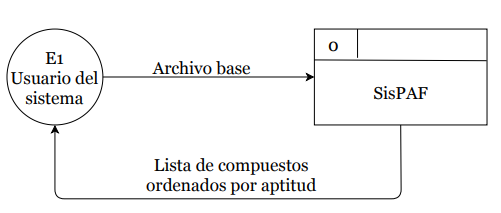
\includegraphics[scale=0.7]{Capitulo2/images/DFDContext.png}
    \caption{Nivel de contexto.}
    \label{nivel contexto}
\end{figure}
%%%%%%%
\begin{figure}[H]
    \centering
    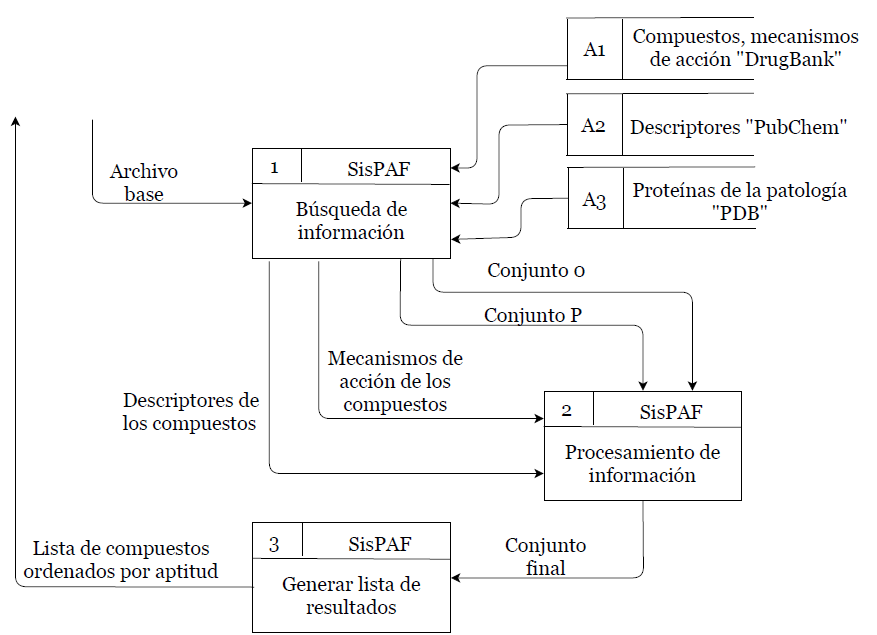
\includegraphics[scale=0.65]{Capitulo2/images/DFDN-1.png}
    \caption{Nivel 1}
    \label{nivel_1}
\end{figure}
%%%%%%%
\begin{figure}[H]
    \centering
    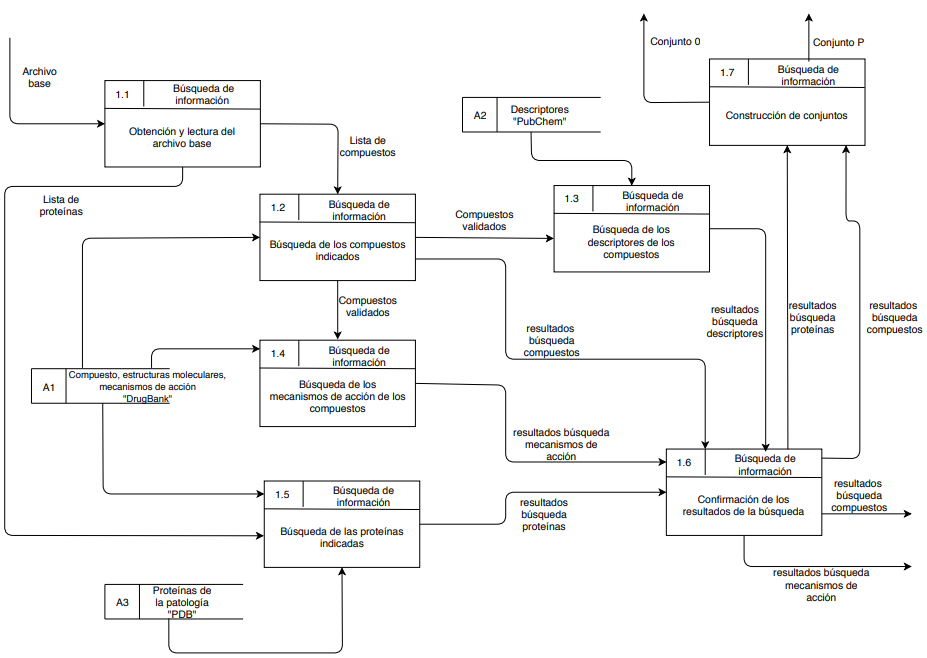
\includegraphics[scale=0.5]{Capitulo2/images/DFD-1.png}
    \caption{Nivel 2 - Requerimiento 1}
    \label{nivel_2_req1}
\end{figure}
%%%%%%%
\begin{figure}[H]
    \centering
    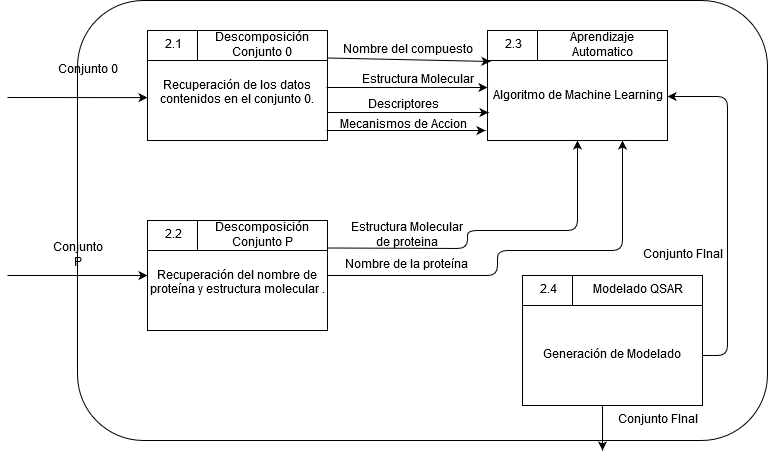
\includegraphics[scale=0.55]{Capitulo2/images/Req2.png}
    \caption{Nivel 2 - Requerimiento 2}
    \label{nivel_2_req2}
\end{figure}
%%%%%%%
\begin{figure}[H]
    \centering
    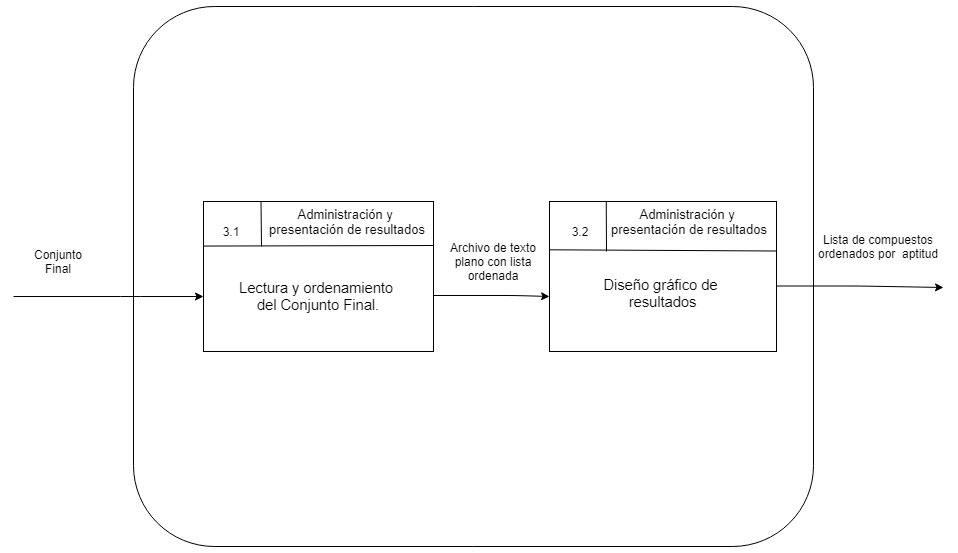
\includegraphics[scale=0.5]{Capitulo2/images/DFD-RF3.png}
    \caption{Nivel 2 - Requerimiento 3}
    \label{nivel_2_req3}
\end{figure}
%%%%%%%
%%%%%%%%%%%%%%%%%%%%%%%%%%%%%%%%%%%%%%%%%%%%%%%
\section{Modelo de Datos}
%%%%%%%%%
\begin{figure}[H]
    \centering
    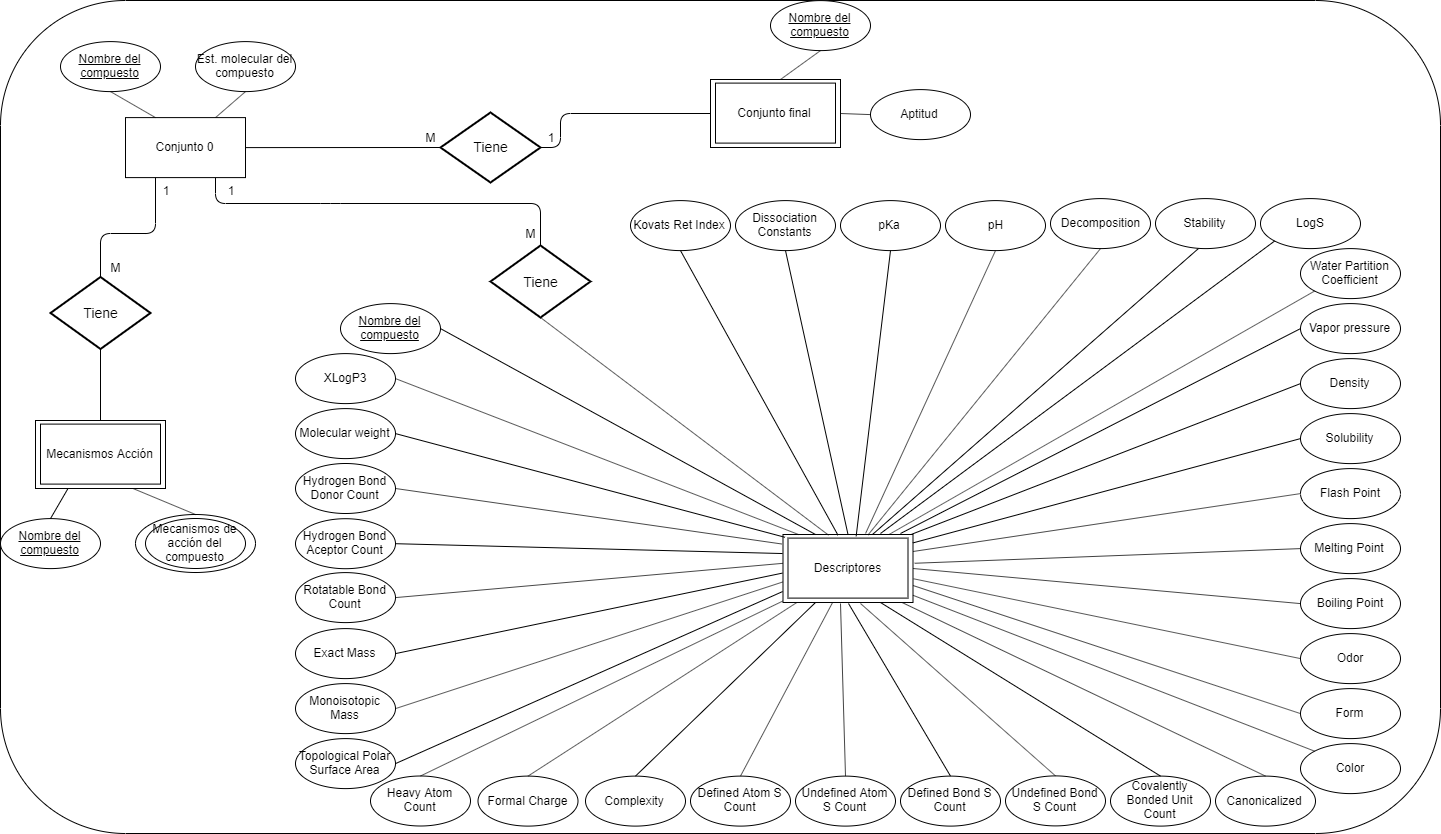
\includegraphics[scale=0.3]{Capitulo2/images/ModeloConceptualDatos.png}
    \caption{Modelo Conceptual de Datos}
    \label{modelo_conceptual}
\end{figure}
%%%%%%%%%
\begin{figure}[H]
    \centering
    \includegraphics[scale=0.4]{Capitulo2/images/modeloDatosLogico.png}
    \caption{Modelo Lógico de Datos}
    \label{fig:my_label}
\end{figure}
%%%%%%%%
%%%%%%%%%%%%%%%%%%%%%%%%%%%%%%%%%%%%%%%%%%%%%%
\section{Interfaces de usuario} 
\noindent La metodología que pone la base en la cual se desarrolla este proyecto, indica una serie de puntos a tomar en cuenta cuando se realiza el prototipado (medio a través del cual se simula el aspecto visual del sistema mediante la representación de los conceptos, componentes, objetos gráficos, entradas y salidas requeridas para la ejecución de cada función en respuesta a las necesidades planteadas), con el fin de conseguir una interfaz eficiente y compatible con las necesidades de los usuarios. Los puntos se indican en la siguiente lista:\\

-	El principal punto que considerar y que constituye la base sobre la que se centra el diseño de prototipos es la identificación de los usuarios a los que va dirigido.\\

-	Analizar las funciones que va a soportar el sistema, con el fin de establecer las dependencias existentes entre ellas y su secuencia de ejecución.
-	Utilizar conceptos, términos y símbolos familiares al usuario, de modo que sea fácil de aprender y comprender.\\

-	Mantener la coherencia dentro del propio sistema y entre sistemas.\\

-	Facilitar la exploración del sistema sin riesgo, permitiendo interrumpir y deshacer las acciones realizadas. De esta forma, el usuario puede utilizar todas las funcionalidades del sistema y trabajar de forma más rápida y eficiente, con la seguridad de que cualquier error puede rectificarse.\\

-	Dificultar la selección de acciones destructivas y no reversibles, pidiéndole verificación de cualquier acción que conlleve un riesgo importante.\\

-	Proporcionar información sobre el estado de ejecución de las funciones, es decir, si la función invocada está en proceso, si se ha completado satisfactoriamente o se ha producido algún error.\\

-	Agrupar las funciones de forma lógica y presentar primero las más utilizadas.\\

-	Buscar la eficiencia en el diálogo evitando cambios frecuentes entre los dispositivos de entrada, tales como el ratón y el teclado.\\

\noindent Una vez tomados en cuenta esos puntos para realizar el diseño, para definir los formatos individuales de las pantallas se realiza un análisis de la información a presentar en cada una de ellas. Este análisis se debe centrar en los siguientes puntos:\\

-	Identificar los diferentes tipos de información como, por ejemplo, campos de datos, títulos, comandos y mensajes de error, con el fin de organizar la pantalla en áreas específicas y conseguir un equilibrio, regularidad, secuencialidad, así́ como, una simetría en la composición de las mismas.\\

-	Estudiar el espacio disponible en las pantallas para determinar qué datos y en qué situación deben aparecer en las mismas, utilizando un formato de visualización que permita al usuario una rápida asimilación de la información.\\

-	Intentar agrupar los datos relacionados y mostrar solo aquellos que son esenciales para la ejecución de la función o para la toma de una decisión, eliminado todas las entradas que sean innecesarias. Nunca se debe pedir al usuario que introduzca información que pueda adquirirse  automáticamente o calcularse internamente.\\

-	Mantener la coherencia entre la entrada y la visualización de datos.\\

-	Proteger al usuario de intentar alguna acción que podría provocar errores, desactivando los comandos que no son operativos en ese contexto.\\

\noindent Todo esto es tomado en cuenta para el prototipado de interfaces y para su futuro desarrollo e implementación en el código.\\

\noindent En esta actividad se especifican las interfaces entre el sistema y el usuario: formatos de
pantallas, diálogos, e informes, principalmente. El objetivo es realizar un análisis de los
procesos del sistema de información en los que se requiere una interacción del usuario, con el
fin de crear una interfaz que satisfaga todos los requisitos establecidos, teniendo en cuenta los
diferentes perfiles a quiénes va dirigido.\\

\noindent Para el desarrollo de interfaces nos basaremos en la ISO 9241 (Proceso de Diseño Centrado en Usuarios) la cual nos proporciona una guía de actividades a través del ciclo de vida de los sistemas interactivos, que consisten en cuatro tipos diferentes de actividades.\\

\noindent• Entender y especificar el contexto de uso.\\
• Especificar los requerimientos de la organización y del usuario.\\
• Proceder a diseñar soluciones.\\
• Evaluar los diseños con respecto a los requerimientos.\\
De las cuales nos enfocaremos en las últimas dos etapas donde se desarrollarán las siguientes actividades:\\

\noindent 1.Realizaremos diseños de prototipos de nuestro producto con el fin de que pueda ser evaluado.\\
2.Se representará cómo los usuarios pueden interactuar con la aplicación o proyecto.\\
3.Crear un plan de evaluación.\\
4.Reportar los resultados de la evaluación y las recomendaciones de cambio.\\
4.1.Iterar esta actividad hasta que el objetivo del diseño sean logrados.\\
Para poder realizar la actividad 3, debemos crear un plan de evaluación, por lo cual nosotros decidimos tomar un plan creado para evaluar interfaces de windows llamada “Windows: GUI Guidelines 4.1” creada por la empresa “ADD Servicios Informáticos S.A”.\\

\noindent Estas recomendaciones fueron implementadas para un proyecto en específico llamado “Proyecto BOE”, por lo cual se hicieron adecuaciones con respecto a nuestro sistema.\\

 \noindent Estos estándares se encuentran definidos y evaluados en la tabla \ref{estandares}, donde se encuentra definida la norma, su tarea y el como aplica en nuestro proyecto.\\

\subsection{Pantallas del sistema}
\noindent Las siguientes pantallas del sistema muestran los procesos mas importantes con las cuales el usuario tendrá que interactuar.
%%%%%%%%%%%%%%%%%%%%%%%%%%%%%%%%%
\begin{figure}[H]
    \centering
    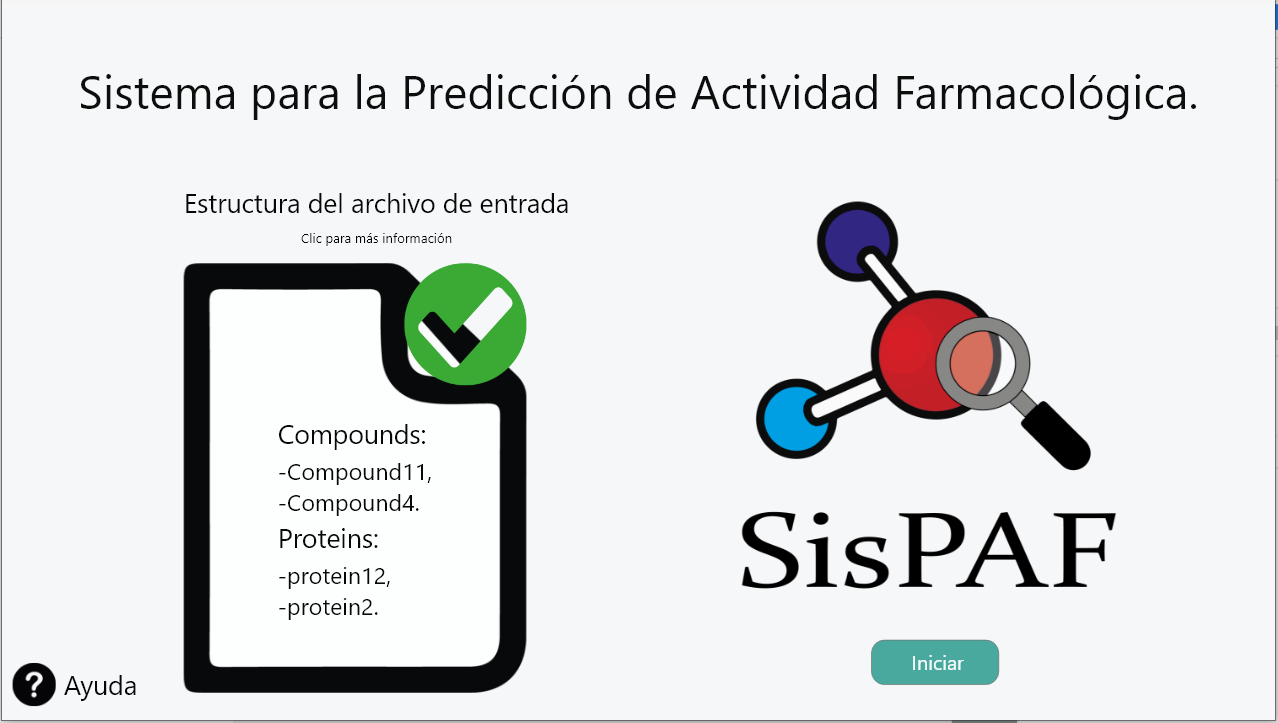
\includegraphics[scale=0.4]{Capitulo2/images/UI/1_tutorial.PNG}
    \caption{Tutorial del archivo base}
    \label{Tutorial_1}
\end{figure}
%%%%%%%%%%%%%%%%%%%%%%%%%%%%%%%
\begin{figure}[H]
    \centering
    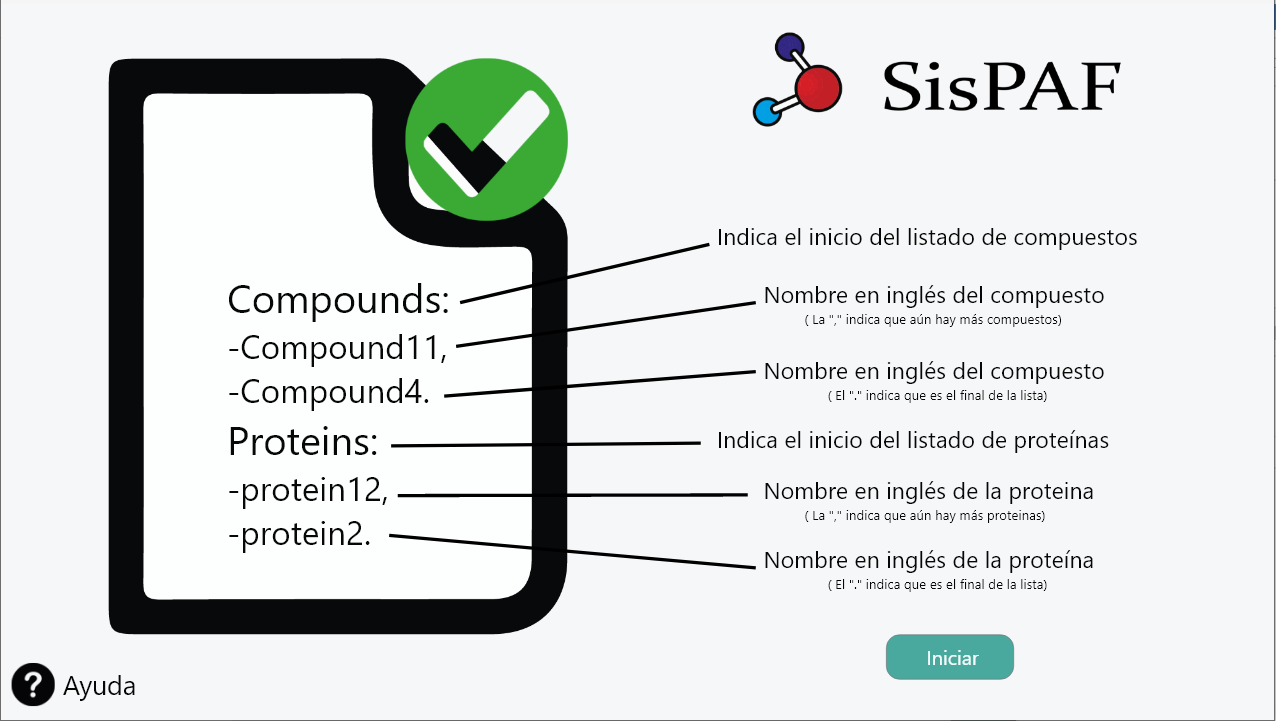
\includegraphics[scale=0.4]{Capitulo2/images/UI/2_tutorial.PNG}
    \caption{Especificación de la estructural del archivo base }
    \label{Tutorial_2}
\end{figure}
%%%%%%%%%%%%%%%%%%%%%%%%%%%%%%
\begin{figure}[H]
    \centering
    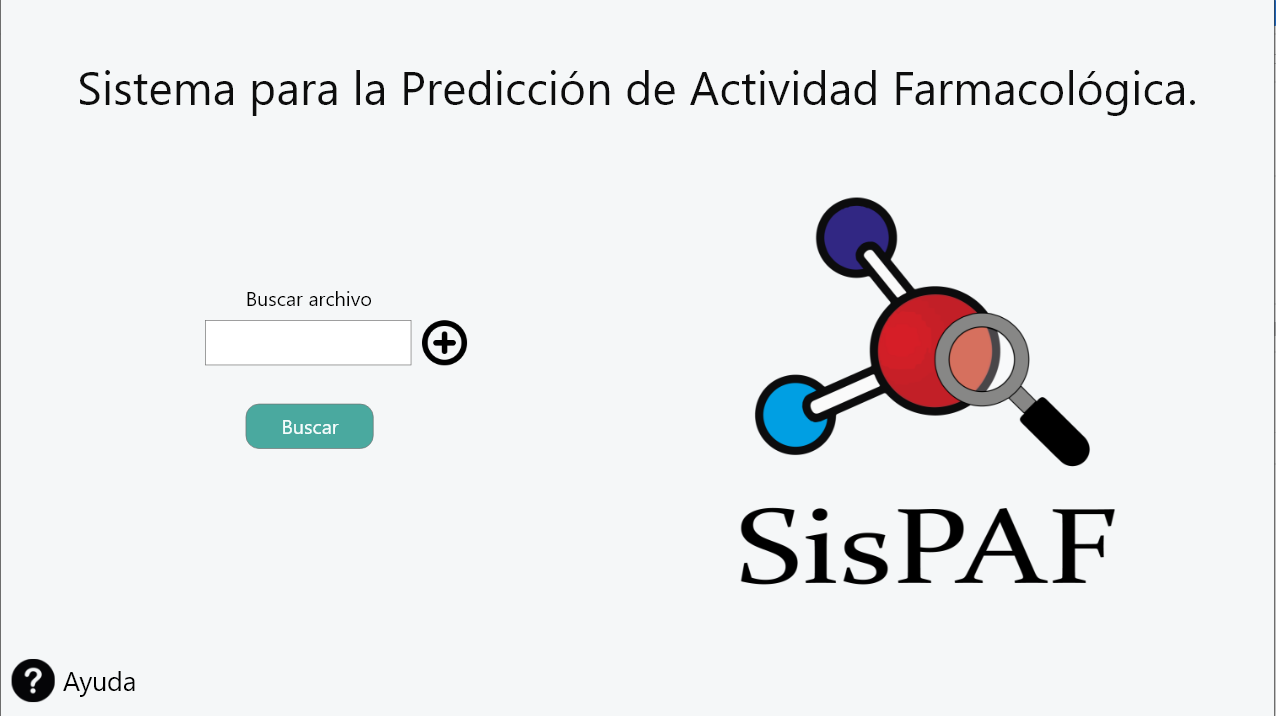
\includegraphics[scale=0.4]{Capitulo2/images/UI/3_pantalla_inicio.PNG}
    \caption{Pantalla de inicio}
    \label{Pantalla_de_inicio}
\end{figure}
%%%%%%%%%%%%%%%%%%%%%%%%%%%%%
\begin{figure}[H]
    \centering
    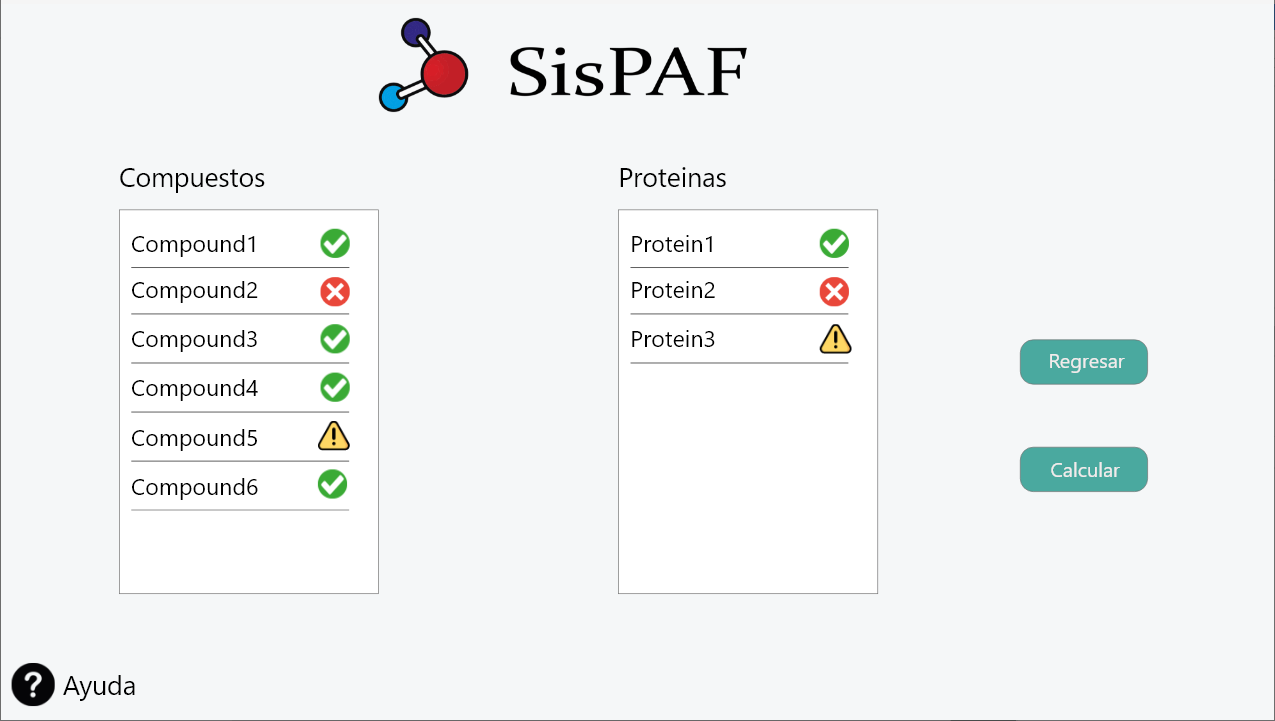
\includegraphics[scale=0.4]{Capitulo2/images/UI/5_preeliminar.PNG}
    \caption{Pantalla preliminar de los elementos encontrados}
    \label{preliminar}
\end{figure}
%%%%%%%%%%%%%%%%%%%%%%%%%%%%%
\begin{figure}[H]
    \centering
    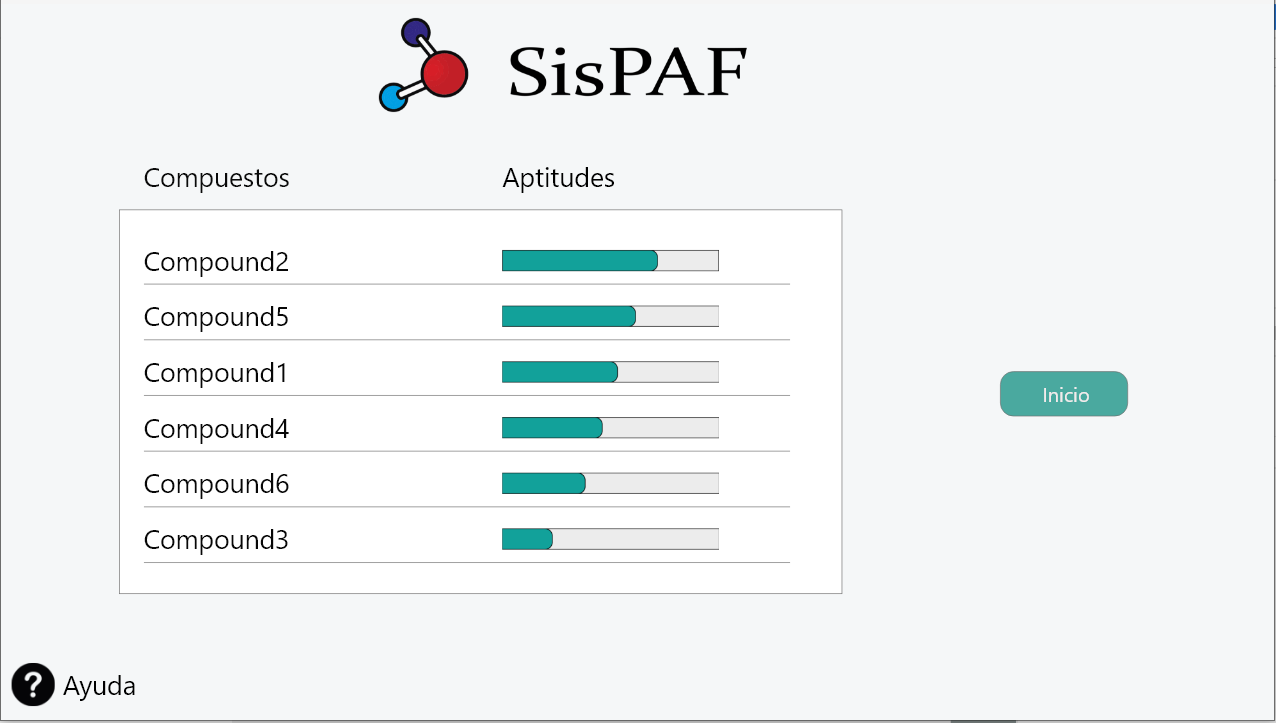
\includegraphics[scale=0.4]{Capitulo2/images/UI/7_resultados.PNG}
    \caption{Resultado arrojado por el sistema (Lista ordenada)}
    \label{Resultados}
\end{figure}
%%%%%%%%%%%%%%%%%%%%%%%%%%%%%
\subsubsection{Pantallas secundarias}
\noindent En este apartado se muestran las pantallas secundarias del sistemas, en la cual solo es cuestión del termino de un proceso interno del sistema. Por lo cual no necesita mayor interacción del usuario.
%%%%%%%%%%%%%%5
\begin{figure}[H]
    \centering
    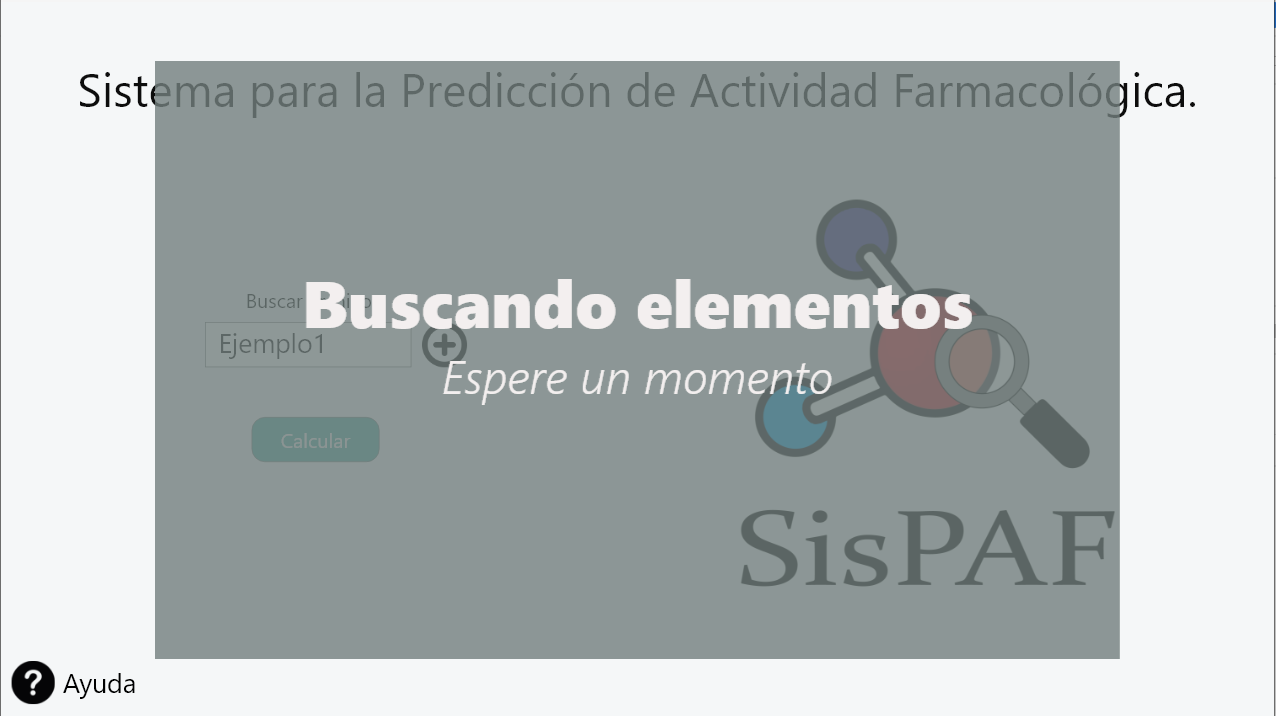
\includegraphics[scale=0.4]{Capitulo2/images/UI/4_Espera_busqueda.PNG}
    \caption{Pantalla de espera mientras la búsqueda de datos se ejecuta}
    \label{Espera_busq}
\end{figure}
%%%%%%%%%%%%%%
\begin{figure}[H]
    \centering
    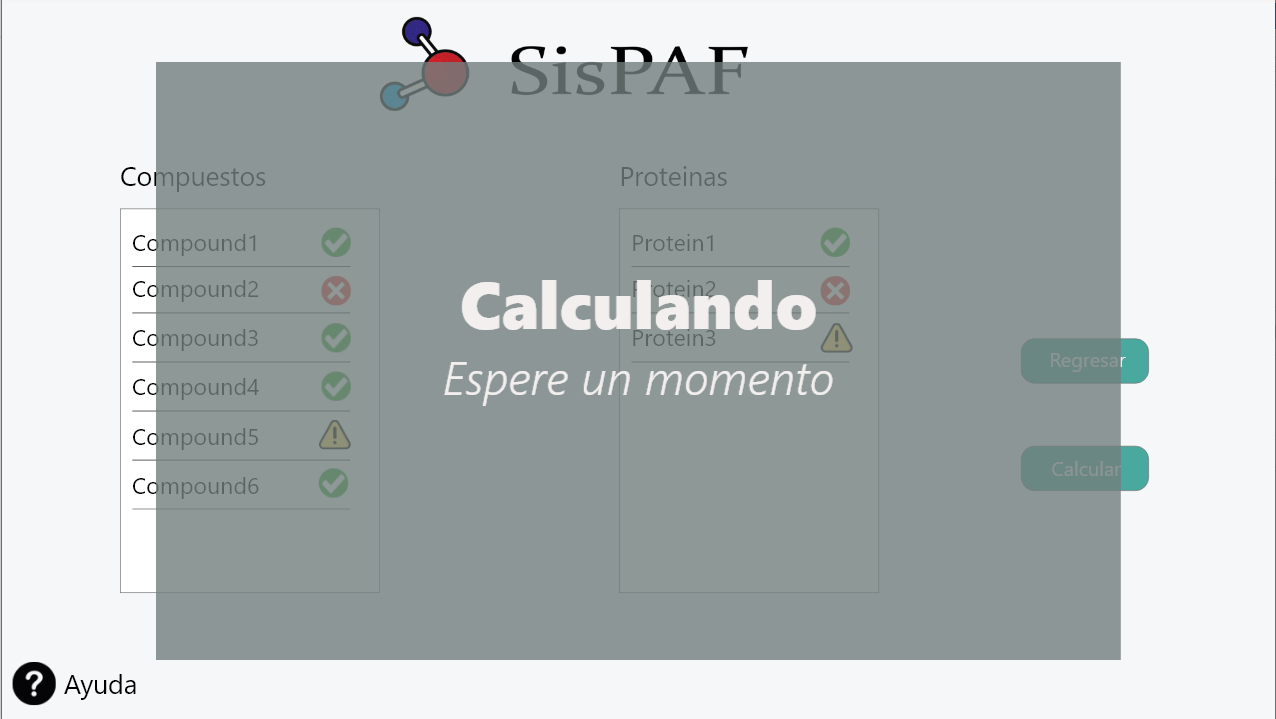
\includegraphics[scale=0.4]{Capitulo2/images/UI/6_espera_calculo.PNG}
    \caption{Pantalla de espera mientras e calculo se efectúa}
    \label{Espera_cal}
\end{figure}
%%%%%%%%%%%%%%%
\subsubsection{Mensajes}
\noindent Estos son los mensajes que se pueden mostrar al usuario por una posible excepción del sistema. 
\begin{figure}[H]
    \centering
    
\includegraphics[scale=0.4]{Capitulo2/images/UI/9_error_conexion.PNG}
    \caption{Mensaje de error de conexión}
    \label{Mensaje_error}
\end{figure}
%%%%%%%%%%%%%%%
\begin{figure}[H]
    \centering
    
\includegraphics[scale=0.4]{Capitulo2/images/UI/10_error_archivo.PNG}
    \caption{Mensaje de error de archivo}
    \label{error_de_Arch}
\end{figure}
%%%%%%%%%%%%%%%%
\begin{figure}[H]
    \centering
    
\includegraphics[scale=0.4]{Capitulo2/images/UI/11_error_datos.PNG}
    \caption{Mensaje de error de datos}
    \label{error_de_datos_notf}
\end{figure}
%%%%%%%%%%%%%%%%
\begin{figure}[H]
    \centering
    
\includegraphics[scale=0.4]{Capitulo2/images/UI/13_advertencia.PNG}
    \caption{Advertencia de datos incompletos}
    \label{advertencia}
\end{figure}

%%%%%%%%%%%%%%%%%%%%%%%%%%%%%%%%%%%%55
\section{Plan de acción}

%Plan de pruebas unitarias
\subsection{Pruebas Unitarias}
\noindent \textbf{Definición:} Verificar la funcionalidad y estructura de cada componente de manera individual.\\
\textbf{Enfoque a usar:} Funcional-Caja negra.\\
\textbf{Descripción:} Se comprueba el correcto funcionamiento de los componentes del sistema de información, analizando las entradas y salidas y verificando que el resultado es el esperado. Se consideran exclusivamente las entradas y salidas del sistema sin preocuparse por la estructura interna del mismo.\\
%%%%%%%%%%%%%%%%%%%%
% Please add the following required packages to your document preamble:
% \usepackage{longtable}
% Note: It may be necessary to compile the document several times to get a multi-page table to line up properly
\begin{longtable}{|l|l|}
\caption{Prueba unitaria RF1.1}
\label{PU_RF1_1}\\
\hline

\textbf{Requerimiento Funcional}                                                       & \textbf{RF1.1 Adquisición del archivo base.}                                                                                                                                                                                                                                                                                                                                                                                                                                                                                                                                                                                                                                                     \\ \hline
\endfirsthead
%
\multicolumn{2}{c}%
{{\bfseries Tabla \thetable\ Continuación de la página anterior}} \\
\endhead
%
\textbf{Perfiles Implicados}                                                           & \begin{tabular}[c]{@{}l@{}}- Desarrollador.\\ - Tester.\end{tabular}                                                                                                                                                                                                                                                                                                                                                                                                                                                                                                                                                                                                                             \\ \hline
\textbf{Planificación temporal}                                                        & \begin{tabular}[c]{@{}l@{}}1. Prueba de compilación.\\ 2. Prueba de funcionamiento.\\ 2.1 Func. botón adquisición archivo.\\ 2.2 Muestra de pantalla selección de\\ archivo.\\ 2.3 Acceso a directorio.\\ 2.4 Carga de archivo.\\ 2.5 Func. botón buscar.\end{tabular}                                                                                                                                                                                                                                                                                                                                                                                                                           \\ \hline
\textbf{Criterio de verificación}                                                      & \begin{tabular}[c]{@{}l@{}}1. Compilación del código.\\ 2. Ejecutable del módulo, hay muestras\\ de que el código hace algo (algo: definido por los \\ siguientes puntos).\\ 2.1 Funcionamiento del botón de Archivo base.\\ 2.2 Visualización de selección de archivo.\\ 2.3 Acceso al directorio correcto o permite acceder \\ a uno distinto desde la pantalla de selección de \\ archivo.\\ 2.4 Carga del archivo correcto.\\ 2.5 El botón se ve adecuadamente y accede al\\ archivo indicado y logra una lectura correcta.\end{tabular}                                                                                                                                                     \\ \hline
\textbf{Criterio de aceptación}                                                        & \begin{tabular}[c]{@{}l@{}}1. No hay errores que impidan la compilación \\ del código.\\ 2. Al usar el ejecutable del módulo, hay muestras \\ de que el código hace algo \\ (algo: definido por los siguientes puntos).\\ 2.1 Se muestra el botón correspondiente, y realiza la \\ acción indicada.\\ 2.2 Es visualizada la pantalla de selección de archivos \\ con cada uno de los componentes.\\ 2.3 La selección de archivos se encuentra en el \\ directorio correcto o permite acceder a uno distinto.\\ 2.4 Solo permite la carga de un archivo de texto \\ plano, y es cargado adecuadamente.\\ 2.5 El botón se ve adecuada, y realiza la acción \\ indicada correctamente.\end{tabular} \\ \hline
\textbf{\begin{tabular}[c]{@{}l@{}}Definición de\\ verificaciones\end{tabular}}        & \begin{tabular}[c]{@{}l@{}}- Errores de Compilación: Ocurren porque la sintaxis \\ del lenguaje no es correcta, de cajón este tipo de \\ errores no permiten que la aplicación se ejecute. \\ \\ - Acción de botón: representa un botón que, cuando \\ es presionado, envía información al que pertenece. \\ La función de  un botón representada  el contenido\\ del elemento.\\ \\ -Visualización de pantalla interfaz de usuario.\end{tabular}                                                                                                                                                                                                                                                \\ \hline
\textbf{\begin{tabular}[c]{@{}l@{}}Análisis y evaluación\\ de resultados\end{tabular}} &                                                                                                                                                                                                                                                                                                                                                                                                                                                                                                                                                                                                                                                                                                  \\ \hline
\textbf{Productos  a entregar}                                                         & \begin{tabular}[c]{@{}l@{}}- Adquisición del archivo base funcionando \\ correctamente.\end{tabular}                                                                                                                                                                                                                                                                                                                                                                                                                                                                                                                                                                                             \\ \hline

\end{longtable}
% Please add the following required packages to your document preamble:
% \usepackage{longtable}
% Note: It may be necessary to compile the document several times to get a multi-page table to line up properly
\begin{longtable}{|l|l|}
\caption{Caso de prueba RF1}
\label{CP_RF1}\\
\hline
\textbf{ID del Caso de prueba}                                                          & CPRF1                                                                                                                                                            \\ \hline
\endfirsthead
%
\multicolumn{2}{c}%
{{\bfseries Tabla \thetable\ Continuación de la página anterior}} \\
\endhead
%
\textbf{Versión}                                                                        & 1.0                                                                                                                                                              \\ \hline
\textbf{Nombre}                                                                         & Caso de prueba para adquisición de archivo base.                                                                                                                 \\ \hline
\textbf{\begin{tabular}[c]{@{}l@{}}Identificador de \\ requerimiento\end{tabular}}      & RF1.1                                                                                                                                                            \\ \hline
\textbf{Propósito}                                                                      & \begin{tabular}[c]{@{}l@{}}Determinar capacidad del sistema para \\ obtener el archivo base.\end{tabular}                                                        \\ \hline
\textbf{Dependencias}                                                                   & N/A                                                                                                                                                              \\ \hline
\textbf{\begin{tabular}[c]{@{}l@{}}Ambiente de \\ prueba/configuración\end{tabular}}    & \begin{tabular}[c]{@{}l@{}}- Hardware: Equipo de computo\\ (preferentemente portatíl)\\ - Software: Compilador python3, \\ IDE y/o editor de texto.\end{tabular} \\ \hline
\textbf{Inicialización}                                                                 & \begin{tabular}[c]{@{}l@{}}- Codificación correspondiente al \\ requerimiento.\\ - Creación del archivo base.\end{tabular}                                       \\ \hline
\textbf{Finalización}                                                                   & N/A                                                                                                                                                              \\ \hline
\textbf{Acciones}                                                                       & \begin{tabular}[c]{@{}l@{}}. Compilar el código correspondiente.\\ - Colocar el archivo en el directorio \\ especificado.\end{tabular}                           \\ \hline
\textbf{\begin{tabular}[c]{@{}l@{}}Descripción de los \\ datos de entrada\end{tabular}} & \begin{tabular}[c]{@{}l@{}}- Archivo de texto plano.\\ - Directorio de la ubicación del archivo base.\end{tabular}                                               \\ \hline
\textbf{Salida esperada}                                                                & \begin{tabular}[c]{@{}l@{}}- Notificación de adecuada adquisición del \\ archivo base.\end{tabular}                                                              \\ \hline
\textbf{Salida obtenida}                                                                &                                                                                                                                                                  \\ \hline
\textbf{Resultado}                                                                      &                                                                                                                                                                  \\ \hline
\textbf{Severidad}                                                                      &                                                                                                                                                                  \\ \hline
\textbf{Evidencia}                                                                      &                                                                                                                                                                  \\ \hline
\textbf{Estado}                                                                         & No Iniciado.                                                                                                                                                     \\ \hline
\end{longtable}

%%%%%%%%%%%%%%%%%%%%
% Please add the following required packages to your document preamble:
% \usepackage{longtable}
% Note: It may be necessary to compile the document several times to get a multi-page table to line up properly
\begin{longtable}{|l|l|}
\caption{Prueba unitaria RF1.2}
\label{PU_RF1_2}\\
\hline
\textbf{Requerimiento Funcional}                                                       & \textbf{RF1.2 Búsqueda de los compuestos indicados..}                                                                                                                                                                                                                                                                                                                                                                                                                                                                                                                                  \\ \hline
\endfirsthead
%
\multicolumn{2}{c}%
{{\bfseries Table \thetable\ Continuación de la página anterior}} \\
\endhead
%
\textbf{Perfiles Implicados}                                                           & \begin{tabular}[c]{@{}l@{}}- Desarrollador.\\ - Tester.\end{tabular}                                                                                                                                                                                                                                                                                                                                                                                                                                                                                                                   \\ \hline
\textbf{Planificación temporal}                                                        & \begin{tabular}[c]{@{}l@{}}1. Prueba de compilación.\\ 2. Prueba de funcionamiento.\\ 2.1 Verificar adecuada lectura del archivo base\\ (token “compunds” ).\\ 2.2 Comprobar conexión a la base de datos \\ “DrugBank”.\\ 2.3 Obtención del .pdb de cada uno de los \\ compuestos enlistados.\\ 2.4 Almacenado del .pdb en el sistema.\end{tabular}                                                                                                                                                                                                                                   \\ \hline
\textbf{Criterio de verificación}                                                      & \begin{tabular}[c]{@{}l@{}}1. Compilación del código.\\ 2. Ejecutable del módulo, hay muestras de que el \\ código hace algo\\ (algo: definido por los siguientes puntos).\\ 2.1 Lectura del token que describe los nombres del\\ compuesto en el archivo base.\\ 2.2 Conexión a  DrugBank y por lo tanto a Internet.\\ 2.3 Adquirir el archivo .pdb del compuesto correcto.\\ 2.4 Almacenamiento de un archivo íntegro en el \\ sistema.\end{tabular}                                                                                                                                \\ \hline
\textbf{Criterio de aceptación}                                                        & \begin{tabular}[c]{@{}l@{}}1. No hay errores que impidan la compilación del \\ código.\\ 2. Al usar el ejecutable del módulo, hay muestras \\ de que el código hace algo\\ (algo: definido por los siguientes puntos).\\ 2.1 No se pierde ningún valor ni dato existente en el\\ archivo base.\\ 2.2 El sistema informa la correcta conexión a \\ “DrugBank”.\\ 2.3 El sistema informa que el compuesto existe \\ en la base de datos y confirma la adquisición \\ del .pdb.\\ 2.4 El sistema notifica la correcta obtención del \\ archivo .pdb y correcto  almacenado.\end{tabular} \\ \hline
\textbf{\begin{tabular}[c]{@{}l@{}}Definición de\\ verificaciones\end{tabular}}        & \begin{tabular}[c]{@{}l@{}}- Errores de Compilación: Ocurren porque la sintaxis \\ del lenguaje no es correcta, de cajón este tipo de \\ errores no permiten que la aplicación se ejecute. \\ \\ - Conexión a base de datos online:Una conexión a \\ base de datos es un archivo de configuración donde \\ se especifica los detalles físicos de una base de datos \\ como por ejemplo el tipo de base de datos y la \\ versión, y los parámetros que permiten una conexión\end{tabular}                                                                                               \\ \hline
\textbf{\begin{tabular}[c]{@{}l@{}}Análisis y evaluación\\ de resultados\end{tabular}} &                                                                                                                                                                                                                                                                                                                                                                                                                                                                                                                                                                                        \\ \hline
\textbf{Productos  a entregar}                                                         & \begin{tabular}[c]{@{}l@{}}- Búsqueda de los compuestos indicados \\ funcionando correctamente.\end{tabular}                                                                                                                                                                                                                                                                                                                                                                                                                                                                           \\ \hline
\end{longtable}
% Please add the following required packages to your document preamble:
% \usepackage{longtable}
% Note: It may be necessary to compile the document several times to get a multi-page table to line up properly
\begin{longtable}{|l|l|}
\caption{Caso de prueba RF1.2}
\label{CP_RF1_2}\\
\hline
\textbf{ID del Caso de prueba}                                                          & CPRF2                                                                                                                                                                                                                                        \\ \hline
\endfirsthead
%
\multicolumn{2}{c}%
{{\bfseries Tabla \thetable\ Continuación de la página anterior}} \\
\endhead
%
\textbf{Versión}                                                                        & 1.0                                                                                                                                                                                                                                          \\ \hline
\textbf{Nombre}                                                                         & \begin{tabular}[c]{@{}l@{}}Caso de prueba para la búsqueda de los \\ compuestos indicados.\end{tabular}                                                                                                                                      \\ \hline
\textbf{\begin{tabular}[c]{@{}l@{}}Identificador de \\ requerimiento\end{tabular}}      & RF1.2                                                                                                                                                                                                                                        \\ \hline
\textbf{Propósito}                                                                      & \begin{tabular}[c]{@{}l@{}}Calificar la búsqueda del compuesto en la base \\ de datos “Drug Bank” , desde obtener el nombre \\ en el archivo base a la adquisición del .pdb.\end{tabular}                                                  \\ \hline
\textbf{Dependencias}                                                                   & Correcta obtención del archivo base.                                                                                                                                                                                                         \\ \hline
\textbf{\begin{tabular}[c]{@{}l@{}}Ambiente de \\ prueba/configuración\end{tabular}}    & \begin{tabular}[c]{@{}l@{}}- Hardware: Equipo de computo\\ (preferentemente portatíl)\\ - Software: Compilador python3, \\ IDE y/o editor de texto.\end{tabular}                                                                             \\ \hline
\textbf{Inicialización}                                                                 & \begin{tabular}[c]{@{}l@{}}- Codificación correspondiente al \\ requerimiento.\\ - Creación del archivo base.\end{tabular}                                                                                                                   \\ \hline
\textbf{Finalización}                                                                   & N/A                                                                                                                                                                                                                                          \\ \hline
\textbf{Acciones}                                                                       & \begin{tabular}[c]{@{}l@{}}. Compilar el código correspondiente.\\ - Contar con el archivo base previamente \\ cargado.\end{tabular}                                                                                                         \\ \hline
\textbf{\begin{tabular}[c]{@{}l@{}}Descripción de los \\ datos de entrada\end{tabular}} & \begin{tabular}[c]{@{}l@{}}- Archivo de texto plano.\\ - Dirección para la conexión a “Drug Bank”.\end{tabular}                                                                                                                              \\ \hline
\textbf{Salida esperada}                                                                & \begin{tabular}[c]{@{}l@{}}Notificación de adecuada estado del \\ compuesto en “Drug Bank” (Existente o no).\\ - De existir, informar que el compuesto \\ existe al igual que el archivo .pdb\\ - Adquisición correcta del .pdb\end{tabular} \\ \hline
\textbf{Salida obtenida}                                                                &                                                                                                                                                                                                                                              \\ \hline
\textbf{Resultado}                                                                      &                                                                                                                                                                                                                                              \\ \hline
\textbf{Severidad}                                                                      &                                                                                                                                                                                                                                              \\ \hline
\textbf{Evidencia}                                                                      &                                                                                                                                                                                                                                              \\ \hline
\textbf{Estado}                                                                         & No Iniciado.                                                                                                                                                                                                                                 \\ \hline
\end{longtable}

%%%%%%%%%%%%%%%%%%%%
% Please add the following required packages to your document preamble:
% \usepackage{longtable}
% Note: It may be necessary to compile the document several times to get a multi-page table to line up properly
\begin{longtable}{|l|l|}
\caption{Prueba unitaria RF1.3}
\label{PU_RF1_3}\\
\hline
\textbf{Requerimiento Funcional}                                                       & \textbf{\begin{tabular}[c]{@{}l@{}}RF1.3 Búsqueda de los descriptores de los \\ compuestos.\end{tabular}}                                                                                                                                                                                                                                                                                                                                                                                                                                                                                                                                                                                                                                                                                                                                                                                      \\ \hline
\endfirsthead
%
\multicolumn{2}{c}%
{{\bfseries Tabla \thetable\ Continuación de la página anterior}} \\
\endhead
%
\textbf{Perfiles Implicados}                                                           & \begin{tabular}[c]{@{}l@{}}- Desarrollador.\\ - Tester.\end{tabular}                                                                                                                                                                                                                                                                                                                                                                                                                                                                                                                                                                                                                                                                                                                                                                                                                           \\ \hline
\textbf{Planificación temporal}                                                        & \begin{tabular}[c]{@{}l@{}}1. Prueba de compilación.\\ 2. Prueba de funcionamiento.\\ 2.1 Verificar que el sistema mantiene el nombre \\ del compuesto sobre del que están obteniendo \\ los datos.\\ 2.2 Comprobar conexión a la base de datos \\ “ChemSpider” y “PubChem”.\\ 2.3 Búsqueda del compuesto en las bases de \\ datos.\\ 2.3.1  Existe el compuesto con el nombre \\ exacto en “PubChem”. \\ 2.3.2 Existe el compuesto con el nombre \\ exacto en “ChemSpider”.\\ 2.4 Adquisición de los descriptores del \\ compuesto en las bases de datos.\\ 2.3.1  Se adquieren  los descriptores  existentes en \\ “PubChem” del compuesto. \\ 2.3.2 Se adquieren  los descriptores  existentes en \\ “ChemSpider” del compuesto.\\ 2.4 Creación del archivo “Descriptors”.\\ 2.5 Almacenado de los datos adquiridos en \\ el archivo correspondiente , recientemente creado.\end{tabular} \\ \hline
\textbf{Criterio de verificación}                                                      & \begin{tabular}[c]{@{}l@{}}1. Compilación del código.\\ 2. Ejecutable del módulo, hay muestras de que el \\ código hace algo\\ (algo: definido por los siguientes puntos).\\ 2.1Verificación de integridad de la variable que \\ contiene el nombre del compuesto.\\ 2.2 Conexión a  “ChemSpider” y “PubChem” \\ y por lo tanto a Internet.\\ 2.3 Adecuada búsqueda del del compuesto exacto \\ en la base de datos.\\ 2.3.1 Correcta adquisición de los descriptores en\\ “PubChem”.\\ 2.3.2 Correcta adquisición de los descriptores en\\ “ChemSpider”.\\ 2.4 Creación del archivo “Descriptors” \\ correspondiente con el compuesto.\\ 2.5 Corroborar guardado de la información \\ obtenida en el archivo creado.\end{tabular}                                                                                                                                                          \\ \hline
\textbf{Criterio de aceptación}                                                        & \begin{tabular}[c]{@{}l@{}}1. No hay errores que impidan la compilación \\ del código.\\ 2. Al usar el ejecutable del módulo, hay muestras \\ de que el código hace algo\\ (algo: definido por los siguientes puntos).\\ 2.1 No se distorsiona el nombre del compuesto \\ de interés.\\ 2.2 El sistema informa la correcta conexión a\\ “ChemSpider”.\\ 2.3 El sistema informa la correcta conexión a \\ “PubChem”.\\ 2.4 El sistema informa que el mismo compuesto \\ existe en ambos repositorios.\\ 2.5. Se notifica la adecuada obtención de los \\ descriptores del compuesto.\\ 2.6 El sistema informa la correcta creación del\\  archivo.\\ 2.7 El archivo y la información que contiene es \\ integra.\end{tabular}                                                                                                                                                                   \\ \hline
\textbf{\begin{tabular}[c]{@{}l@{}}Definición de\\ verificaciones\end{tabular}}        & \begin{tabular}[c]{@{}l@{}}- Errores de Compilación: Ocurren porque la \\ sintaxis del lenguaje no es correcta, de cajón \\ este tipo de errores no permiten que la \\ aplicación se ejecute. \\ \\ - Conexión a base de datos online: \\ Una conexión a base de datos es un archivo \\ de configuración donde se especifica los \\ detalles físicos de una base de datos como por \\ ejemplo el tipo de base de datos y la versión, y \\ los parámetros que permiten una conexión\end{tabular}                                                                                                                                                                                                                                                                                                                                                                                                \\ \hline
\textbf{\begin{tabular}[c]{@{}l@{}}Análisis y evaluación\\ de resultados\end{tabular}} & - Resultados:                                                                                                                                                                                                                                                                                                                                                                                                                                                                                                                                                                                                                                                                                                                                                                                                                                                                                  \\ \hline
\textbf{Productos  a entregar}                                                         & \begin{tabular}[c]{@{}l@{}}- Búsqueda de los descriptores correspondientes\\  al compuesto de interés.\end{tabular}                                                                                                                                                                                                                                                                                                                                                                                                                                                                                                                                                                                                                                                                                                                                                                            \\ \hline
\end{longtable}
% Please add the following required packages to your document preamble:
% \usepackage{longtable}
% Note: It may be necessary to compile the document several times to get a multi-page table to line up properly
\begin{longtable}{|l|l|}
\caption{Caso de prueba RF1.3}
\label{CP_RF1_3}\\
\hline
\textbf{ID del Caso de prueba}                                                          & CPRF3                                                                                                                                                                                                                                                          \\ \hline
\endfirsthead
%
\multicolumn{2}{c}%
{{\bfseries Tabla \thetable\ Continuación de la página anterior}} \\
\endhead
%
\textbf{Versión}                                                                        & 1.0                                                                                                                                                                                                                                                            \\ \hline
\textbf{Nombre}                                                                         & \begin{tabular}[c]{@{}l@{}}Caso de prueba para la búsqueda de los \\ descriptores de los compuestos.\end{tabular}                                                                                                                                              \\ \hline
\textbf{\begin{tabular}[c]{@{}l@{}}Identificador de \\ requerimiento\end{tabular}}      & RF1.3                                                                                                                                                                                                                                                          \\ \hline
\textbf{Propósito}                                                                      & \begin{tabular}[c]{@{}l@{}}Identificar el funcionamiento del sistema al \\ momento de conectarse a las dos bases de datos \\ contenedoras de descriptores de compuestos, \\ “ChemSpider” y “PubChem”.\end{tabular}                                             \\ \hline
\textbf{Dependencias}                                                                   & Correcta obtención del archivo base.                                                                                                                                                                                                                           \\ \hline
\textbf{\begin{tabular}[c]{@{}l@{}}Ambiente de \\ prueba/configuración\end{tabular}}    & \begin{tabular}[c]{@{}l@{}}- Hardware: Equipo de computo\\ (preferentemente portatíl)\\ - Software: Compilador python3, \\ IDE y/o editor de texto.\end{tabular}                                                                                               \\ \hline
\textbf{Inicialización}                                                                 & \begin{tabular}[c]{@{}l@{}}- Codificación correspondiente al \\ requerimiento.\\ - Creación del archivo base.\end{tabular}                                                                                                                                     \\ \hline
\textbf{Finalización}                                                                   & N/A                                                                                                                                                                                                                                                            \\ \hline
\textbf{Acciones}                                                                       & \begin{tabular}[c]{@{}l@{}}. Compilar el código correspondiente.\\ - Contar con el archivo base previamente \\ cargado.\end{tabular}                                                                                                                           \\ \hline
\textbf{\begin{tabular}[c]{@{}l@{}}Descripción de los \\ datos de entrada\end{tabular}} & \begin{tabular}[c]{@{}l@{}}- Nombre del compuesto.\\ - Dirección para la conexión a \\ “ChemSpider” y “PubChem”.\end{tabular}                                                                                                                                  \\ \hline
\textbf{Salida esperada}                                                                & \begin{tabular}[c]{@{}l@{}}- Notificación de adecuada estado del \\ compuesto en\\ “ChemSpider” y “PubChem”. (Existente o no).\\ - De existir, informar que el compuesto existe \\ al igual que el archivo .pdb\\ - Adquisición correcta del .pdb\end{tabular} \\ \hline
\textbf{Salida obtenida}                                                                &                                                                                                                                                                                                                                                                \\ \hline
\textbf{Resultado}                                                                      &                                                                                                                                                                                                                                                                \\ \hline
\textbf{Severidad}                                                                      &                                                                                                                                                                                                                                                                \\ \hline
\textbf{Evidencia}                                                                      &                                                                                                                                                                                                                                                                \\ \hline
\textbf{Estado}                                                                         & No Iniciado.                                                                                                                                                                                                                                                   \\ \hline
\end{longtable}

%%%%%%%%%%%%%%%%%%%
% Please add the following required packages to your document preamble:
% \usepackage{longtable}
% Note: It may be necessary to compile the document several times to get a multi-page table to line up properly
\begin{longtable}{|l|l|}
\caption{Prueba unitaria RF1.4}
\label{PU_RF1_4}\\
\hline
\textbf{Requerimiento Funcional}                                                       & \textbf{\begin{tabular}[c]{@{}l@{}}RF1.4 Búsqueda de los mecanismos de \\acción de los compuestos.\end{tabular}}                                                                                                                                                                                                                                                                                                                                                                                                                                                                                                                                                                                                                                                                                                         \\ \hline
\endfirsthead
%
\multicolumn{2}{c}%
{{\bfseries Tabla \thetable\ Continuación de la página anterior}} \\
\endhead
%
\textbf{Perfiles Implicados}                                                           & \begin{tabular}[c]{@{}l@{}}- Desarrollador.\\ - Tester.\end{tabular}                                                                                                                                                                                                                                                                                                                                                                                                                                                                                                                                                                                                                                                                                                                                                        \\ \hline
\textbf{Planificación temporal}                                                        & \begin{tabular}[c]{@{}l@{}}1. Prueba de compilación.\\ 2. Prueba de funcionamiento.\\ 2.1 Verificar que el sistema mantiene el nombre \\ del compuesto sobre del que están obteniendo \\ los datos.\\ 2.2 Comprobar estado de la conexión a la base \\ de datos “DrugBank”.\\ 2.3 Comprobar que se mantiene la dirección\\ correspondiente  a el compuesto sobre el que \\ se está trabajando.\\ 2.4 Adquisición de la representación cuantitativa  \\ de la actividad biológica del compuesto en la \\ bases de datos “DrugBank”. \\ 2.5 Creación del archivo “BioActivity”.\\ 2.6 Almacenado de los datos adquiridos en el \\ archivo correspondiente , recientemente creado.\end{tabular}                                                                                                                                \\ \hline
\textbf{Criterio de verificación}                                                      & \begin{tabular}[c]{@{}l@{}}1. Compilación del código.\\ 2. Ejecutable del módulo, hay muestras de que el \\ código hace algo\\ (algo: definido por los siguientes puntos).\\ 2.1Verificación de integridad de la variable que \\ contiene el nombre del compuesto.\\ 2.2 Conexión a  “DrugBank” y por lo tanto a \\ Internet.\\ 2.3 Adecuada búsqueda del compuesto exacto \\ en la base de datos.\\ 2.4 Correcta adquisición de las cantidades \\ descriptivas de la actividad biológica en \\ “DrugBank”.\\ 2.5 Creación del archivo “BioActivity” \\ correspondiente con el compuesto.\\ 2.6 Corroborar guardado de la información \\ obtenida en el archivo creado\end{tabular}                                                                                                                                       \\ \hline
\textbf{Criterio de aceptación}                                                        & \begin{tabular}[c]{@{}l@{}}1. No hay errores que impidan la compilación \\ del código.\\ 2. Al usar el ejecutable del módulo, hay \\ muestras de que el código hace algo\\ (algo: definido por los siguientes puntos).\\ 2.1 No se distorsiona el nombre del compuesto \\ de interés.\\ 2.2 El sistema informa la correcta conexión a \\ “DrugBank”.\\ 2.3. Se notifica la adecuada obtención de los \\ datos cuantitativos de la actividad biológica \\ del compuesto.\\ 2.4 El sistema informa la correcta creación \\ del archivo.\\ 2.5 Son guardados todos los datos obtenidos \\ de DrugBank en el archivo creado.\end{tabular}                                                                                                                                                                                       \\ \hline
\textbf{\begin{tabular}[c]{@{}l@{}}Definición de\\ verificaciones\end{tabular}}        & \begin{tabular}[c]{@{}l@{}}- Errores de Compilación: Ocurren porque \\ la sintaxis del lenguaje no es correcta, de \\ cajón este tipo de errores no permiten que \\ la aplicación se ejecute. \\ \\ - Conexión a base de datos online: Una conexión \\ a base de datos es un archivo de configuración \\ donde se especifica los detalles físicos de una \\ base de datos como por ejemplo el tipo de \\ base de datos y la versión, y los parámetros que \\ permiten una conexión.\\ \\ - Manejo de Archivos: Un programa no puede \\ manipular los datos de un archivo directamente. \\ Para usar un archivo, un programa siempre \\ abrir el archivo y asignarlo a una variable, que \\ llamaremos el archivo lógico. Todas las \\ operaciones sobre un archivo se realizan a través \\ del archivo lógico.\end{tabular} \\ \hline
\textbf{\begin{tabular}[c]{@{}l@{}}Análisis y evaluación\\ de resultados\end{tabular}} & - Resultados:                                                                                                                                                                                                                                                                                                                                                                                                                                                                                                                                                                                                                                                                                                                                                                                                               \\ \hline
\textbf{Productos  a entregar}                                                         & \begin{tabular}[c]{@{}l@{}}-Búsqueda de la actividad biológica del \\ compuesto de interés funcionando correctamente.\end{tabular}                                                                                                                                                                                                                                                                                                                                                                                                                                                                                                                                                                                                                                                                                          \\ \hline
\end{longtable}
% Please add the following required packages to your document preamble:
% \usepackage{longtable}
% Note: It may be necessary to compile the document several times to get a multi-page table to line up properly
\begin{longtable}{|l|l|}
\caption{Caso de prueba RF1.4}
\label{CP_RF_4}\\
\hline
\textbf{ID del Caso de prueba}                                                          & CPRF4                                                                                                                                                                                                                                                                                                                         \\ \hline
\endfirsthead
%
\multicolumn{2}{c}%
{{\bfseries Tabla \thetable\ Continuación de la página anterior}} \\
\endhead
%
\textbf{Versión}                                                                        & 1.0                                                                                                                                                                                                                                                                                                                           \\ \hline
\textbf{Nombre}                                                                         & \begin{tabular}[c]{@{}l@{}}Caso de prueba para la búsqueda de los \\ mecanismos de acción de los compuestos.\end{tabular}                                                                                                                                                                                                             \\ \hline
\textbf{\begin{tabular}[c]{@{}l@{}}Identificador de \\ requerimiento\end{tabular}}      & RF1.4                                                                                                                                                                                                                                                                                                                         \\ \hline
\textbf{Propósito}                                                                      & \begin{tabular}[c]{@{}l@{}}Identificar el funcionamiento del sistema al \\ momento de re-conectarse o mantenerse conectado\\ a la base de datos contenedora de los datos \\ cuantitativos representantes de la actividad \\ biológica de los compuestos, “DrugBank”.\end{tabular}                                            \\ \hline
\textbf{Dependencias}                                                                   & \begin{tabular}[c]{@{}l@{}}- Correcta obtención del archivo base.\\ - Correcta adquisición de la estructura molecular \\ del compuesto.\\ - Adecuada conexión de la base de datos \\ “DrugBank”.\end{tabular}                                                                                                                 \\ \hline
\textbf{\begin{tabular}[c]{@{}l@{}}Ambiente de \\ prueba/configuración\end{tabular}}    & \begin{tabular}[c]{@{}l@{}}- Hardware: Equipo de computo\\ (preferentemente portatíl)\\ - Software: Compilador python3, \\ IDE y/o editor de texto.\end{tabular}                                                                                                                                                              \\ \hline
\textbf{Inicialización}                                                                 & \begin{tabular}[c]{@{}l@{}}- Codificación correspondiente al \\ requerimiento.\\ - Creación del archivo base.\end{tabular}                                                                                                                                                                                                    \\ \hline
\textbf{Finalización}                                                                   & N/A                                                                                                                                                                                                                                                                                                                           \\ \hline
\textbf{Acciones}                                                                       & \begin{tabular}[c]{@{}l@{}}. Compilar el código correspondiente.\\ - Contar con el archivo base previamente \\ cargado.\end{tabular}                                                                                                                                                                                          \\ \hline
\textbf{\begin{tabular}[c]{@{}l@{}}Descripción de los \\ datos de entrada\end{tabular}} & \begin{tabular}[c]{@{}l@{}}- Nombre del compuesto.\\ - Dirección para la conexión a “DrugBank”.\end{tabular}                                                                                                                                                                                                                  \\ \hline
\textbf{Salida esperada}                                                                & \begin{tabular}[c]{@{}l@{}}- Notificación de adecuada estado del \\ compuesto en “DrugBank”. (Existente o no).\\ - De existir, informar la adecuada obtención \\ de los datos que conforman la actividad \\ biológica del compuesto.\\ - Informar correcta creación del archivo \\ “BioActivity” y su contenido.\end{tabular} \\ \hline
\textbf{Salida obtenida}                                                                &                                                                                                                                                                                                                                                                                                                               \\ \hline
\textbf{Resultado}                                                                      &                                                                                                                                                                                                                                                                                                                               \\ \hline
\textbf{Severidad}                                                                      &                                                                                                                                                                                                                                                                                                                               \\ \hline
\textbf{Evidencia}                                                                      &                                                                                                                                                                                                                                                                                                                               \\ \hline
\textbf{Estado}                                                                         & No Iniciado.                                                                                                                                                                                                                                                                                                                  \\ \hline
\end{longtable}

%%%%%%%%%%%%%%%%%%%
% Please add the following required packages to your document preamble:
% \usepackage{longtable}
% Note: It may be necessary to compile the document several times to get a multi-page table to line up properly
\begin{longtable}{|l|l|}
\caption{Prueba unitaria RF1.5}
\label{PU_RF1_5}\\
\hline
\textbf{Requerimiento Funcional}                                                       & \textbf{RF1.5 Búsqueda de las proteínas indicadas.}                                                                                                                                                                                                                                                                                                                                                                                                                                                                                                                                                                                                                                                                                                                                                                                                                                                                                                                                       \\ \hline
\endfirsthead
%
\multicolumn{2}{c}%
{{\bfseries Tabla \thetable\ Continuación de la página anterior}} \\
\endhead
%
\textbf{Perfiles Implicados}                                                           & \begin{tabular}[c]{@{}l@{}}- Desarrollador.\\ - Tester.\end{tabular}                                                                                                                                                                                                                                                                                                                                                                                                                                                                                                                                                                                                                                                                                                                                                                                                                                                                                                                      \\ \hline
\textbf{Planificación temporal}                                                        & \begin{tabular}[c]{@{}l@{}}1. Prueba de compilación.\\ 2. Prueba de funcionamiento.\\ 2.1 Func. botón adquisición archivo.\\ 2.2 Muestra de pantalla selección de archivo.\\ 2.3 Acceso a directorio.\\ 2.4 Carga de archivo.\\ 2.5 Func. botón buscar.\\ 2.6 Conexión a PDB\\ 2.7 Búsqueda del compuesto en la base de datos.\\ 2.8 Adquisición de la estructura molecular \\ correspondiente al  compuesto.\\ 2.9 Creación del archivo “Proteins”.\\ 2.10 Guardado de los datos en el archivo creado.\end{tabular}                                                                                                                                                                                                                                                                                                                                                                                                                                                                      \\ \hline
\textbf{Criterio de verificación}                                                      & \begin{tabular}[c]{@{}l@{}}1. Compilación del código.\\ 2. Ejecutable del módulo, hay muestras de que \\ el código hace algo \\ (algo: definido por los siguientes puntos).\\ 2.1 Funcionamiento del botón de Archivo base.\\ 2.2 Visualización de selección de archivo.\\ 2.3 Acceso al directorio correcto o permite \\ acceder a uno distinto desde la pantalla de \\ selección de archivo.\\ 2.4 Carga del archivo correcto.\\ 2.5 El botón se ve adecuadamente y accede al \\ archivo indicado y logra una lectura correcta.\\ 2.6 Funciona la accion del boton logrando la \\ correcta conexión a la base de datos PDB\\ 2.7 Búsqueda del compuesto en PDB.\\ 2.8 Adquisición de la estructura molecular del \\ archivo .pdb\\ 2.9 Creación del archivo “Proteins”\\ 2.10 Almacenado de la estructura molecular \\ en el archivo creado.\end{tabular}                                                                                                                               \\ \hline
\textbf{Criterio de aceptación}                                                        & \begin{tabular}[c]{@{}l@{}}1. No hay errores que impidan la compilación \\ del código.\\ 2. Al usar el ejecutable del módulo, hay muestras \\ de que el código hace algo\\ (algo: definido por los siguientes puntos).\\ 2.1 Se muestra el botón correspondiente, \\ y realiza la acción indicada.\\ 2.2 Es visualizada la pantalla de selección de \\ archivos con cada uno de los componentes.\\ 2.3 La selección de archivos se encuentra en el \\ directorio correcto o permite acceder a uno \\ distinto. \\ 2.4 Solo permite la carga de un archivo de texto \\ plano, y es cargado adecuadamente.\\ 2.5 El botón se ve adecuada, y realiza la acción \\ indicada correctamente. \\ 2.6 Se comprueba la adecuada conexión a PDB.\\ 2.7 Búsqueda adecuada del compuesto en PDB.\\ 2.8 Verificar que se creó correctamente el archivo\\ “Proteins”\\ 2.9 Adecuada adquisición de la estructura \\ molecular, para posteriormente ser almacenada \\ en el archivo creado.\end{tabular} \\ \hline
\textbf{\begin{tabular}[c]{@{}l@{}}Definición de\\ verificaciones\end{tabular}}        & \begin{tabular}[c]{@{}l@{}}- Errores de Compilación: Ocurren porque la \\ sintaxis del lenguaje no es correcta, de cajón \\ este tipo de errores no permiten que la \\ aplicación se ejecute. \\ \\ - Acción de botón: representa un botón que, \\ cuando es presionado, envía información al que \\ pertenece. La función de  un botón representada  \\ el contenido del elemento.\\ \\ - Visualización de pantalla interfaz de usuario.\\ \\  - Manejo de Archivos: Un programa no puede \\ manipular los datos de un archivo directamente. \\ Para usar un archivo, un programa siempre abrir \\ el archivo y asignarlo a una variable, que \\ llamaremos el archivo lógico. Todas las\\ operaciones sobre un archivo se realizan \\ a través del archivo lógico.\end{tabular}                                                                                                                                                                                                         \\ \hline
\textbf{\begin{tabular}[c]{@{}l@{}}Análisis y evaluación\\ de resultados\end{tabular}} & - Resultados:                                                                                                                                                                                                                                                                                                                                                                                                                                                                                                                                                                                                                                                                                                                                                                                                                                                                                                                                                                             \\ \hline
\textbf{Productos  a entregar}                                                         & \begin{tabular}[c]{@{}l@{}}Adquisición del archivo base funcionando \\ correctamente.\end{tabular}                                                                                                                                                                                                                                                                                                                                                                                                                                                                                                                                                                                                                                                                                                                                                                                                                                                                                        \\ \hline
\end{longtable}
% Please add the following required packages to your document preamble:
% \usepackage{longtable}
% Note: It may be necessary to compile the document several times to get a multi-page table to line up properly
\begin{longtable}{|l|l|}
\caption{Caso de prueba RF1.5}
\label{CP_RF1_5}\\
\hline
\textbf{ID del Caso de prueba}                                                          & CPRF5                                                                                                                                                                                                                                        \\ \hline
\endfirsthead
%
\multicolumn{2}{c}%
{{\bfseries Tabla \thetable\ Continuación de la página anterior}} \\
\endhead
%
\textbf{Versión}                                                                        & 1.0                                                                                                                                                                                                                                          \\ \hline
\textbf{Nombre}                                                                         & Caso de prueba para adquisición de archivo base.                                                                                                                                                                                             \\ \hline
\textbf{\begin{tabular}[c]{@{}l@{}}Identificador de \\ requerimiento\end{tabular}}      & RF1.5                                                                                                                                                                                                                                        \\ \hline
\textbf{Propósito}                                                                      & \begin{tabular}[c]{@{}l@{}}Identificar el funcionamiento del sistema al obtener \\ el archivo que contiene el nombre de las proteínas, \\ la obtención de su estructura molecular a partir de \\ la conexión establecida a PDB.\end{tabular} \\ \hline
\textbf{Dependencias}                                                                   & - Correcta obtención del archivo base.                                                                                                                                                                                                       \\ \hline
\textbf{\begin{tabular}[c]{@{}l@{}}Ambiente de \\ prueba/configuración\end{tabular}}    & \begin{tabular}[c]{@{}l@{}}- Hardware: Equipo de computo\\ (preferentemente portatíl)\\ - Software: Compilador python3, \\ IDE y/o editor de texto.\end{tabular}                                                                             \\ \hline
\textbf{Inicialización}                                                                 & \begin{tabular}[c]{@{}l@{}}- Codificación correspondiente al \\ requerimiento.\\ - Creación del archivo base.\end{tabular}                                                                                                                   \\ \hline
\textbf{Finalización}                                                                   & N/A                                                                                                                                                                                                                                          \\ \hline
\textbf{Acciones}                                                                       & \begin{tabular}[c]{@{}l@{}}. Compilar el código correspondiente.\\ - Contar con el archivo base previamente \\ cargado.\end{tabular}                                                                                                         \\ \hline
\textbf{\begin{tabular}[c]{@{}l@{}}Descripción de los \\ datos de entrada\end{tabular}} & \begin{tabular}[c]{@{}l@{}}- Nombre de la proteina.\\ -Dirección para la conexión a “PDB”.\end{tabular}                                                                                                                                      \\ \hline
\textbf{Salida esperada}                                                                & \begin{tabular}[c]{@{}l@{}}- Notificación de adecuada estado del \\ compuesto en  “PDB”.(Existente o no).\\ - De existir, informar que el compuesto \\ existe al igual que el archivo .pdb\\ - Adquisición correcta del .pdb\end{tabular}    \\ \hline
\textbf{Salida obtenida}                                                                &                                                                                                                                                                                                                                              \\ \hline
\textbf{Resultado}                                                                      &                                                                                                                                                                                                                                              \\ \hline
\textbf{Severidad}                                                                      &                                                                                                                                                                                                                                              \\ \hline
\textbf{Evidencia}                                                                      &                                                                                                                                                                                                                                              \\ \hline
\textbf{Estado}                                                                         & No Iniciado.                                                                                                                                                                                                                                 \\ \hline
\end{longtable}

%%%%%%%%%%%%%%%%%%%
% Please add the following required packages to your document preamble:
% \usepackage{longtable}
% Note: It may be necessary to compile the document several times to get a multi-page table to line up properly
\begin{longtable}{|l|l|}
\caption{Prueba unitaria RF1.6}
\label{PU_RF1_6}\\
\hline
\textbf{Requerimiento Funcional}                                                       & \textbf{\begin{tabular}[c]{@{}l@{}}RF1.6  Confirmación de los resultados de la\\ búsqueda.\end{tabular}}                                                                                                                                                                                                                                                                                                                                                                                                                                                                                                                                                                                                                                                                                                                                                                                                                                                                                                               \\ \hline
\endfirsthead
%
\multicolumn{2}{c}%
{{\bfseries Tabla \thetable\ Continuación de la página anterior}} \\
\endhead
%
\textbf{Perfiles Implicados}                                                           & \begin{tabular}[c]{@{}l@{}}- Desarrollador.\\ - Tester.\end{tabular}                                                                                                                                                                                                                                                                                                                                                                                                                                                                                                                                                                                                                                                                                                                                                                                                                                                                                                                                                   \\ \hline
\textbf{Planificación temporal}                                                        & \begin{tabular}[c]{@{}l@{}}1. Prueba de compilación.\\ 2. Prueba de funcionamiento.\\ 2.1 Verificar despliegue de la interfaz que \\ informa el fin de adquisición de datos.\\ 2.2 Chequeo en que el sistema contemple los \\ directorios donde se encuentran cada uno de los \\ archivos creados.\\ 2.2.1 Existencia del directorio y de los archivos\\ correspondientes a la estructura molecular del \\ compuesto.\\ 2.2.2 Existencia del directorio y de los archivos\\ correspondientes a los descriptores del compuesto.\\ 2.2.3 Existencia del directorio y de los archivos\\ correspondientes a la actividad biológica del \\ compuesto.\\ 2.2.4 Existencia del directorio y del archivo \\ correspondiente a la(s) proteina(s)\\ 2.5 Interfaz que indica estado de cada uno de los \\ archivos.\\ 2.5.1 Se indica si la estructura del archivo es \\ correcta con el contenido adecuado.\\ 2.5.2 Se notifica si existe un error en el archivo,\\ especificando este, así como la posible causa.\end{tabular} \\ \hline
\textbf{Criterio de verificación}                                                      & \begin{tabular}[c]{@{}l@{}}1. Compilación del código.\\ 2. Ejecutable del módulo, hay muestras de que \\ el código hace algo\\ (algo: definido por los siguientes puntos).\\ 2.1 Verificación de integridad en los archivos \\ creados para cada uno de los datos perteneciente \\ a los compuestos.\\ 2.2 Rectificar la cantidad de archivos creados \\ para cada compuesto, y que estos coinciden con \\ los estimados.\\ 2.3 Verificación de la creación y estructura \\ adecuada del archivo que contiene la estructura \\ de cada una de la(s) proteínas.\\ 2.4 Chequeo a las pantallas que muestran los \\ resultados para la adquisición de información.\\ 2.5 Aparición en el momento indicado de \\ mensajes que indiquen algún error, falla o \\ información que requiera saber el usuario.\\ 2.4 Creación del archivo “\\ Descriptors” correspondiente con el compuesto.\\ 2.5 Corroborar guardado de la información \\ obtenida en el archivo creado.\end{tabular}                                      \\ \hline
\textbf{Criterio de aceptación}                                                        & \begin{tabular}[c]{@{}l@{}}1. No hay errores que impidan la compilación \\ del código.\\ 2. Al usar el ejecutable del módulo, hay muestras \\ de que el código hace algo\\ (algo: definido por los siguientes puntos).\\ 2.1 No se distorsiona el nombre del compuesto \\ de interés.\\ 2.2 El sistema informa la correcta conexión a\\ “ChemSpider”.\\ 2.3 El sistema informa la correcta conexión a\\ “PubChem”.\\ 2.4 El sistema informa que el mismo compuesto \\ existe en ambos repositorios.\\ 2.5. Se notifica la adecuada obtención de los \\ descriptores del compuesto.\\ 2.6 El sistema informa la correcta creación \\ del archivo.\\ 2.7 El archivo y la información que contiene \\ es integra.\end{tabular}                                                                                                                                                                                                                                                                                            \\ \hline
\textbf{\begin{tabular}[c]{@{}l@{}}Definición de\\ verificaciones\end{tabular}}        & \begin{tabular}[c]{@{}l@{}}- Errores de Compilación: Ocurren porque la \\ sintaxis del lenguaje no es correcta, de cajón \\ este tipo de errores no permiten que la \\ aplicación se ejecute. \\ \\ - Acción de botón: representa un botón que, \\ cuando es presionado, envía información al que \\ pertenece. La función de  un botón representada  \\ el contenido del elemento.\\ \\ - Visualización de pantalla interfaz de usuario.\\ \\  - Manejo de Archivos: Un programa no puede \\ manipular los datos de un archivo directamente. \\ Para usar un archivo, un programa siempre abrir \\ el archivo y asignarlo a una variable, que \\ llamaremos el archivo lógico. Todas las\\ operaciones sobre un archivo se realizan \\ a través del archivo lógico.\end{tabular}                                                                                                                                                                                                                                      \\ \hline
\textbf{\begin{tabular}[c]{@{}l@{}}Análisis y evaluación\\ de resultados\end{tabular}} & - Resultados:                                                                                                                                                                                                                                                                                                                                                                                                                                                                                                                                                                                                                                                                                                                                                                                                                                                                                                                                                                                                          \\ \hline
\textbf{Productos  a entregar}                                                         & \begin{tabular}[c]{@{}l@{}}- Confirmación de los resultados de la búsqueda \\ funcionando correctamente.\end{tabular}                                                                                                                                                                                                                                                                                                                                                                                                                                                                                                                                                                                                                                                                                                                                                                                                                                                                                                  \\ \hline
\end{longtable}
% Please add the following required packages to your document preamble:
% \usepackage{longtable}
% Note: It may be necessary to compile the document several times to get a multi-page table to line up properly
\begin{longtable}{|l|l|}
\caption{Caso de prueba RF1.6}
\label{CP_RF1_6}\\
\hline
\textbf{ID del Caso de prueba}                                                          & CPRF6                                                                                                                                                                                                                                                                    \\ \hline
\endfirsthead
%
\multicolumn{2}{c}%
{{\bfseries Tabla \thetable\ Continuación de la página anterior}} \\
\endhead
%
\textbf{Versión}                                                                        & 1.0                                                                                                                                                                                                                                                                      \\ \hline
\textbf{Nombre}                                                                         & Confirmación de los resultados de la búsqueda.                                                                                                                                                                                                                           \\ \hline
\textbf{\begin{tabular}[c]{@{}l@{}}Identificador de \\ requerimiento\end{tabular}}      & RF1.6                                                                                                                                                                                                                                                                    \\ \hline
\textbf{Propósito}                                                                      & \begin{tabular}[c]{@{}l@{}}Rectificar el funcionamiento del sistema para \\ indicar el estatus de la información obtenida de \\ los previos requerimientos referente a\\ compuestos y proteína(s) de interés.\end{tabular}                                               \\ \hline
\textbf{Dependencias}                                                                   & \begin{tabular}[c]{@{}l@{}}Correcta obtención de la información necesaria \\ de los compuestos y la requerida para la(s) \\ proteína(s) objetivo.\end{tabular}                                                                                                           \\ \hline
\textbf{\begin{tabular}[c]{@{}l@{}}Ambiente de \\ prueba/configuración\end{tabular}}    & \begin{tabular}[c]{@{}l@{}}- Hardware: Equipo de computo\\ (preferentemente portatíl)\\ - Software: Compilador python3, \\ IDE y/o editor de texto.\end{tabular}                                                                                                         \\ \hline
\textbf{Inicialización}                                                                 & \begin{tabular}[c]{@{}l@{}}- Codificación correspondiente al \\ requerimiento.\\ - Previa realización de la pruebas  de los\\  RF previos, especialmente para trabajar \\ bajo la creación de los archivos \\ correspondientes de a compuestos y proteinas.\end{tabular} \\ \hline
\textbf{Finalización}                                                                   & N/A                                                                                                                                                                                                                                                                      \\ \hline
\textbf{Acciones}                                                                       & \begin{tabular}[c]{@{}l@{}}- Compilar el código correspondiente.\\ - Contar con los archivos creados \\ previamente (compuesto y proteína(s)).\end{tabular}                                                                                                              \\ \hline
\textbf{\begin{tabular}[c]{@{}l@{}}Descripción de los \\ datos de entrada\end{tabular}} & \begin{tabular}[c]{@{}l@{}}- Nombre del compuesto.\\ - Directorio de los archivos \\ correspondiente a los compuestos.\\ - Directorio de los archivos que \\ pertenecen a la(s) proteína(s).\end{tabular}                                                                \\ \hline
\textbf{Salida esperada}                                                                & \begin{tabular}[c]{@{}l@{}}- Notificación de los estados de cada uno de\\  los archivos, dependiendo de su origen, ya sea \\ de un compuesto o de una proteína.\end{tabular}                                                                                             \\ \hline
\textbf{Salida obtenida}                                                                &                                                                                                                                                                                                                                                                          \\ \hline
\textbf{Resultado}                                                                      &                                                                                                                                                                                                                                                                          \\ \hline
\textbf{Severidad}                                                                      &                                                                                                                                                                                                                                                                          \\ \hline
\textbf{Evidencia}                                                                      &                                                                                                                                                                                                                                                                          \\ \hline
\textbf{Estado}                                                                         & No Iniciado.                                                                                                                                                                                                                                                             \\ \hline
\end{longtable}

%%%%%%%%%%%%%%%%%%%
% Please add the following required packages to your document preamble:
% \usepackage{longtable}
% Note: It may be necessary to compile the document several times to get a multi-page table to line up properly
\begin{longtable}{|l|l|}
\caption{Prueba unitaria RF1.7.1}
\label{PU_RF1_7_1}\\
\hline
\textbf{Requerimiento Funcional}                                                       & \textbf{RF1.7.1 Construcción del conjunto cero.}                                                                                                                                                                                                                                                                                                                                                                                                                                                                                                                                                                                                                                                                                                                                                                                            \\ \hline
\endfirsthead
%
\multicolumn{2}{c}%
{{\bfseries Tabla \thetable\ Continuación de la página anterior}} \\
\endhead
%
\textbf{Perfiles Implicados}                                                           & \begin{tabular}[c]{@{}l@{}}- Desarrollador.\\ - Tester.\end{tabular}                                                                                                                                                                                                                                                                                                                                                                                                                                                                                                                                                                                                                                                                                                                                                                        \\ \hline
\textbf{Planificación temporal}                                                        & \begin{tabular}[c]{@{}l@{}}1. Prueba de compilación.\\ 2. Prueba de funcionamiento.\\ 2.1 Verificar que no existió errores en la \\ obtención de información.\\ 2.2 Comprobar adecuada estructura de cada \\ uno de los archivos que conforman el conjunto 0.\\ 2.3 Chequeo de la correcta apertura  y lectura \\ de cada uno de los archivos creados por proteína \\ del listado.\\ 2.4 Creación del archivo que se define como \\ conjunto0, que contendrá toda la información \\ respecto a descriptores.\\ 2.5  Verificación por cada iteración el cambio \\ al archivo correspondiente para agregar la \\ información necesaria, especialmente que no \\ existe pérdida de información.\end{tabular}                                                                                                                                 \\ \hline
\textbf{Criterio de verificación}                                                      & \begin{tabular}[c]{@{}l@{}}1. Compilación del código.\\ 2. Ejecutable del módulo, hay muestras de que \\ el código hace algo\\ (algo: definido por los siguientes puntos).\\ 2.1 Verificación de errores en la adquisición de \\ datos de cada uno de  los compuestos.\\ 2.2 Revisión de la estructura en cada uno de \\ los archivos pertenecientes a cada compuesto de \\ la lista (Archivo base).\\ 2.3 Lectura de los archivos de los cuales se \\ extraerán los datos que contiene el conjunto0.\\ 2.4 Creación del archivo conjunto0.\\ 2.5 Modificación por cada iteración del archivo\\ conjunto0, en el que se agrega datos de cada \\ compuesto.\end{tabular}                                                                                                                                                                    \\ \hline
\textbf{Criterio de aceptación}                                                        & \begin{tabular}[c]{@{}l@{}}1. No hay errores que impidan la compilación \\ del código.\\ 2. Al usar el ejecutable del módulo, hay muestras \\ de que el código hace algo\\ (algo: definido por los siguientes puntos).\\ 2.1El sistema notifica la adquisición correcta o \\ incorrecta la adquisición completa de los datos \\ referentes a los compuestos.\\ 2.2El sistema muestra mensajes de error, en \\ caso de presentarse alguna falla en los archivos \\ contenedores de datos.\\ 2.3 El sistema accede y lee adecuadamente cada \\ uno de los archivos.\\ 2.4 El sistema informa adecuada creación del \\ conjunto 0 o muestra el error en caso de existir.\\ 2.5. Informa errores en el caso de existir al \\ crear el contenido del conjunto 0.\\ 2.6 El sistema informa la correcta estructura \\ del conjunto0\end{tabular} \\ \hline
\textbf{\begin{tabular}[c]{@{}l@{}}Definición de\\ verificaciones\end{tabular}}        & \begin{tabular}[c]{@{}l@{}}- Errores de Compilación: Ocurren porque la \\ sintaxis del lenguaje no es correcta, de cajón \\ este tipo de errores no permiten que la \\ aplicación se ejecute. \\ \\ - Visualización de pantalla interfaz de usuario.\\ \\  - Manejo de Archivos: Un programa no puede \\ manipular los datos de un archivo directamente. \\ Para usar un archivo, un programa siempre abrir \\ el archivo y asignarlo a una variable, que \\ llamaremos el archivo lógico. Todas las\\ operaciones sobre un archivo se realizan \\ a través del archivo lógico.\end{tabular}                                                                                                                                                                                                                                                \\ \hline
\textbf{\begin{tabular}[c]{@{}l@{}}Análisis y evaluación\\ de resultados\end{tabular}} & - Resultados:                                                                                                                                                                                                                                                                                                                                                                                                                                                                                                                                                                                                                                                                                                                                                                                                                               \\ \hline
\textbf{Productos  a entregar}                                                         & \begin{tabular}[c]{@{}l@{}}- Búsqueda de los compuestos indicados \\ funcionando correctamente.\end{tabular}                                                                                                                                                                                                                                                                                                                                                                                                                                                                                                                                                                                                                                                                                                                                \\ \hline
\end{longtable}
% Please add the following required packages to your document preamble:
% \usepackage{longtable}
% Note: It may be necessary to compile the document several times to get a multi-page table to line up properly
\begin{longtable}{|l|l|}
\caption{Caso de prueba RF1.7.1}
\label{CP_RF1_7}\\
\hline
\textbf{ID del Caso de prueba}                                                          & CPRF7                                                                                                                                                                            \\ \hline
\endfirsthead
%
\multicolumn{2}{c}%
{{\bfseries Tabla \thetable\ Continuación de la página anterior}} \\
\endhead
%
\textbf{Versión}                                                                        & 1.0                                                                                                                                                                              \\ \hline
\textbf{Nombre}                                                                         & Caso de prueba para adquisición de archivo base.                                                                                                                                 \\ \hline
\textbf{\begin{tabular}[c]{@{}l@{}}Identificador de \\ requerimiento\end{tabular}}      & RF1.7.1                                                                                                                                                                          \\ \hline
\textbf{Propósito}                                                                      & \begin{tabular}[c]{@{}l@{}}Identificar el funcionamiento del sistema al \\ crear el archivo “conjunto0” que posee la \\ información de cada uno de los compuestos.\end{tabular}  \\ \hline
\textbf{Dependencias}                                                                   & \begin{tabular}[c]{@{}l@{}}Correcta obtención de la información necesaria \\ de los compuestos y la requerida para la(s) \\ proteína(s) objetivo.\end{tabular}                   \\ \hline
\textbf{\begin{tabular}[c]{@{}l@{}}Ambiente de \\ prueba/configuración\end{tabular}}    & \begin{tabular}[c]{@{}l@{}}- Hardware: Equipo de computo\\ (preferentemente portatíl)\\ - Software: Compilador python3, \\ IDE y/o editor de texto.\end{tabular}                 \\ \hline
\textbf{Inicialización}                                                                 & \begin{tabular}[c]{@{}l@{}}- Codificación correspondiente al \\ requerimiento.\\ - Directorio y existencia de los \\ archivos correspondiente a los compuestos.\end{tabular}     \\ \hline
\textbf{Finalización}                                                                   & N/A                                                                                                                                                                              \\ \hline
\textbf{Acciones}                                                                       & \begin{tabular}[c]{@{}l@{}}- Compilar el código correspondiente.\\ - Contar con los archivos creados para \\ cada uno de los datos de interés de cada \\ compuesto.\end{tabular} \\ \hline
\textbf{\begin{tabular}[c]{@{}l@{}}Descripción de los \\ datos de entrada\end{tabular}} & \begin{tabular}[c]{@{}l@{}}- Nombre del compuesto.\\ - Directorio y nombre de cada uno de los \\ archivos para el o los compuesto(s).\end{tabular}                               \\ \hline
\textbf{Salida esperada}                                                                & \begin{tabular}[c]{@{}l@{}}- Notificación de adecuada existencia \\ de los archivos para cada compuesto.\end{tabular}                                                            \\ \hline
\textbf{Salida obtenida}                                                                &                                                                                                                                                                                  \\ \hline
\textbf{Resultado}                                                                      &                                                                                                                                                                                  \\ \hline
\textbf{Severidad}                                                                      &                                                                                                                                                                                  \\ \hline
\textbf{Evidencia}                                                                      &                                                                                                                                                                                  \\ \hline
\textbf{Estado}                                                                         & No Iniciado.                                                                                                                                                                     \\ \hline
\end{longtable}

%%%%%%%%%%%%%%%%%%%
% Please add the following required packages to your document preamble:
% \usepackage{longtable}
% Note: It may be necessary to compile the document several times to get a multi-page table to line up properly
\begin{longtable}{|l|l|}
\caption{Prueba unitaria RF2.1}
\label{PU_RF2_1}\\
\hline
\textbf{Requerimiento Funcional}                                                       & \textbf{\begin{tabular}[c]{@{}l@{}}RF 2.1 Adquisición y descomposición \\ del conjunto 0.\end{tabular}}                                                                                                                                                                                                                                                                                                                                                                                                                                                                                                                                                                                                                                                                                                                                                                                                                     \\ \hline
\endfirsthead
%
\multicolumn{2}{c}%
{{\bfseries Tabla \thetable\ Continuación de la página anterior}} \\
\endhead
%
\textbf{Perfiles Implicados}                                                           & \begin{tabular}[c]{@{}l@{}}- Desarrollador.\\ - Tester.\end{tabular}                                                                                                                                                                                                                                                                                                                                                                                                                                                                                                                                                                                                                                                                                                                                                                                                                                                        \\ \hline
\textbf{Planificación temporal}                                                        & \begin{tabular}[c]{@{}l@{}}1. Prueba de compilación.\\ 2. Prueba de funcionamiento.\\ 2.1 Verificar que el sistema reconoce el \\ conjunto 0 y puede acceder a este.\\ 2.2 Comprobar lectura adecuada del \\ conjunto 0.\\ 2.3 Adquisición de información por medio \\ del contenido de conjunto 0.\\ 2.4 Reconocer que la información se adquiere por \\ iteración, y pertenece únicamente a un compuesto. \\ 2.5. Adquisición de los datos y transferencia a \\ variables.\end{tabular}                                                                                                                                                                                                                                                                                                                                                                                                                                   \\ \hline
\textbf{Criterio de verificación}                                                      & \begin{tabular}[c]{@{}l@{}}1. Compilación del código.\\ 2. Ejecutable del módulo, hay muestras de que \\ el código hace algo\\ (algo: definido por los siguientes puntos).\\ 2.1Verificación de acceso a directorio y \\ archivo “conjunto0”.\\ 2.2 Comprobar lectura adecuada del \\ “conjunto0”.\\ 2.3 Revisión de la creación de variables para \\ manejo de los datos de compuestos por parte \\ del sistema.\\ 2.3.1 Verificación de integridad y adecuado \\ valor de las  variables creadas.\end{tabular}                                                                                                                                                                                                                                                                                                                                                                                                            \\ \hline
\textbf{Criterio de aceptación}                                                        & \begin{tabular}[c]{@{}l@{}}1. No hay errores que impidan la compilación \\ del código.\\ 2. Al usar el ejecutable del módulo, hay muestras \\ de que el código hace algo(\\ algo: definido por los siguientes puntos).\\ 2.1 Se encuentra fácilmente el archivo “conjunto0” \\ y el sistema informa al usuario que se obtuvo \\ adecuadamente, o en caso contrario, muestra \\ la causa de error.\\ 2.2 El sistema puede leer el archivo”conjunto0”\\ 2.3 El sistema adquiere y guarda en variables \\ la información contenida en el “conjunto0”.\\ 2.4 Se comprueba que el manejo de la variables \\ que contienen información pueden ser usadas \\ fácilmente.\end{tabular}                                                                                                                                                                                                                                              \\ \hline
\textbf{\begin{tabular}[c]{@{}l@{}}Definición de\\ verificaciones\end{tabular}}        & \begin{tabular}[c]{@{}l@{}}- Errores de Compilación: Ocurren porque la \\ sintaxis del lenguaje no es correcta, de cajón \\ este tipo de errores no permiten que la \\ aplicación se ejecute. \\ - Variables de programación: La variable está \\ formada por un espacio en el sistema de almacenaje \\ (memoria principal de un ordenador) y un nombre \\ simbólico (un identificador) que está asociado \\ a dicho espacio. Ese espacio contiene una cantidad \\ de información conocida o desconocida, es decir \\ un valor.\\  - Visualización de pantalla interfaz de usuario.\\   - Manejo de Archivos: Un programa no puede \\ manipular los datos de un archivo directamente. \\ Para usar un archivo, un programa siempre abrir \\ el archivo y asignarlo a una variable, que \\ llamaremos el archivo lógico. Todas las\\ operaciones sobre un archivo se realizan \\ a través del archivo lógico.\end{tabular} \\ \hline
\textbf{\begin{tabular}[c]{@{}l@{}}Análisis y evaluación\\ de resultados\end{tabular}} & - Resultados:                                                                                                                                                                                                                                                                                                                                                                                                                                                                                                                                                                                                                                                                                                                                                                                                                                                                                                               \\ \hline
\textbf{Productos  a entregar}                                                         & \begin{tabular}[c]{@{}l@{}}- Adquisición y descomposición del \\ conjunto 0 funcionando correctamente.\end{tabular}                                                                                                                                                                                                                                                                                                                                                                                                                                                                                                                                                                                                                                                                                                                                                                                                         \\ \hline
\end{longtable}
% Please add the following required packages to your document preamble:
% \usepackage{longtable}
% Note: It may be necessary to compile the document several times to get a multi-page table to line up properly
\begin{longtable}{|l|l|}
\caption{Caso de prueba RF2.1}
\label{CP_RF2_1}\\
\hline
\textbf{ID del Caso de prueba}                                                          & CPRF9                                                                                                                                                                          \\ \hline
\endfirsthead
%
\multicolumn{2}{c}%
{{\bfseries Tabla \thetable\ Continuación de la página anterior}} \\
\endhead
%
\textbf{Versión}                                                                        & 1.0                                                                                                                                                                            \\ \hline
\textbf{Nombre}                                                                         & \begin{tabular}[c]{@{}l@{}}Caso de prueba para Adquisición\\  y descomposición del conjunto0.\end{tabular}                                                                     \\ \hline
\textbf{\begin{tabular}[c]{@{}l@{}}Identificador de \\ requerimiento\end{tabular}}      & RF2.1                                                                                                                                                                          \\ \hline
\textbf{Propósito}                                                                      & \begin{tabular}[c]{@{}l@{}}- Identificar el funcionamiento del sistema \\ para adquirir el conjunto0 y \\ descomponerlo en datos.\end{tabular}                                 \\ \hline
\textbf{Dependencias}                                                                   & - Correcta creación del conjunto0                                                                                                                                              \\ \hline
\textbf{\begin{tabular}[c]{@{}l@{}}Ambiente de \\ prueba/configuración\end{tabular}}    & \begin{tabular}[c]{@{}l@{}}- Hardware: Equipo de computo\\ (preferentemente portatíl)\\ - Software: Compilador python3, \\ IDE y/o editor de texto.\end{tabular}               \\ \hline
\textbf{Inicialización}                                                                 & \begin{tabular}[c]{@{}l@{}}- Codificación correspondiente al requerimiento.\\ - Carga  del archivo base.\end{tabular}                                                          \\ \hline
\textbf{Finalización}                                                                   & N/A                                                                                                                                                                            \\ \hline
\textbf{Acciones}                                                                       & \begin{tabular}[c]{@{}l@{}}- Compilar el código correspondiente.\\ - Contar con el archivo conjunto0\\  creado.\end{tabular}                                                   \\ \hline
\textbf{\begin{tabular}[c]{@{}l@{}}Descripción de los \\ datos de entrada\end{tabular}} & \begin{tabular}[c]{@{}l@{}}- Directorio del conjunto0\\ - Adquisición de dicho archivo.\end{tabular}                                                                           \\ \hline
\textbf{Salida esperada}                                                                & \begin{tabular}[c]{@{}l@{}}- Notificación de correcta lectura del \\ conjunto0\\ - El sistema informa que adquirió correctamente \\ la información del conjunto0.\end{tabular} \\ \hline
\textbf{Salida obtenida}                                                                &                                                                                                                                                                                \\ \hline
\textbf{Resultado}                                                                      &                                                                                                                                                                                \\ \hline
\textbf{Severidad}                                                                      &                                                                                                                                                                                \\ \hline
\textbf{Evidencia}                                                                      &                                                                                                                                                                                \\ \hline
\textbf{Estado}                                                                         & No Iniciado.                                                                                                                                                                   \\ \hline
\end{longtable}

%%%%%%%%%%%%%%%%%%%
% Please add the following required packages to your document preamble:
% \usepackage{longtable}
% Note: It may be necessary to compile the document several times to get a multi-page table to line up properly
\begin{longtable}{|l|l|}
\caption{Prueba unitaria RF2.2}
\label{PU_RF_2_2}\\
\hline
\textbf{Requerimiento Funcional}                                                        & \textbf{\begin{tabular}[c]{@{}l@{}}RF 2.2 Adquisición y descomposición \\ del conjuntoP.\end{tabular}}                                                                                                                                                                                                                                                                                                                                                                                                                                                                                                                                                                                                                                                                                                                                                                                                                   \\ \hline
\endfirsthead
%
\multicolumn{2}{c}%
{{\bfseries Tabla \thetable\ Continuación de la página anterior}} \\
\endhead
%
\textbf{Perfiles Implicados}                                                            & \begin{tabular}[c]{@{}l@{}}- Desarrollador.\\ - Tester.\end{tabular}                                                                                                                                                                                                                                                                                                                                                                                                                                                                                                                                                                                                                                                                                                                                                                                                                                                     \\ \hline
\textbf{Planificación temporal}                                                         & \begin{tabular}[c]{@{}l@{}}1. Prueba de compilación.\\ 2. Prueba de funcionamiento.\\ 2.1 Verificar que el sistema reconoce el \\ conjuntoP\\  y puede acceder a este.\\ 2.2 Comprobar lectura adecuada del \\ conjuntoP.\\ 2.3 Adquisición de información por medio del \\ contenido de conjuntoP.\\ 2.4 Reconocer que la información se adquiere \\ por iteración, y pertenece únicamente a un \\ compuesto. \\ 2.5. Adquisición de los datos y \\ transferencia a variables.\end{tabular}                                                                                                                                                                                                                                                                                                                                                                                                                             \\ \hline
\textbf{Criterio de verificación}                                                       & \begin{tabular}[c]{@{}l@{}}- Compilación del código.\\ - Ejecutable del módulo, hay muestras de que \\ el código hace algo\\ (algo: definido por los siguientes puntos).\\ 2.1 Verificación de acceso a directorio y archivo \\ conjuntoP.\\ 2.2 Comprobar lectura adecuada del \\ conjuntoP.\\ 2.3 Revisión de la creación de variables para \\ manejo de los datos de compuestos por parte \\ del sistema.\\ 2.3.1 Verificación de integridad y adecuado \\ valor de las  variables creadas.\end{tabular}                                                                                                                                                                                                                                                                                                                                                                                                              \\ \hline
\textbf{Criterio de aceptación}                                                         & \begin{tabular}[c]{@{}l@{}}1. No hay errores que impidan la compilación \\ del código.\\ 2. Al usar el ejecutable del módulo, hay muestras \\ de que el código hace algo\\ (algo: definido por los siguientes puntos).\\ 2.1 Se encuentra fácilmente el archivo conjuntoP\\  y el sistema informa al usuario que se obtuvo \\ adecuadamente, o en caso contrario, muestra la \\ causa de error.\\ 2.2 El sistema puede leer el archivo conjuntoP.\\ 2.3 El sistema adquiere y guarda en variables la \\ información contenida en el conjuntoP.\\ 2.4 Se comprueba que el manejo de la variables \\ que contienen información pueden ser usadas \\ fácilmente.\end{tabular}                                                                                                                                                                                                                                               \\ \hline
\textbf{Definición de verificaciones}                                                   & \begin{tabular}[c]{@{}l@{}}- Errores de Compilación: Ocurren porque la \\ sintaxis del lenguaje no es correcta, de cajón \\ este tipo de errores no permiten que la \\ aplicación se ejecute. \\ - Variables de programación:la variable está \\ formada por un espacio en el sistema de \\ almacenaje (memoria principal de un ordenador) \\ y un nombre simbólico (un identificador) que \\ está asociado a dicho espacio. Ese espacio \\ contiene una cantidad de información \\ conocida o desconocida, es decir un valor.\\ - Visualización de pantalla interfaz de usuario.\\  - Manejo de Archivos: Un programa no \\ puede manipular los datos de un archivo \\ directamente. Para usar un archivo, un\\ programa siempre abrir el archivo y \\ asignarlo a una variable, que llamaremos \\ el archivo lógico. Todas las operaciones sobre \\ un archivo se realizan a través del\\ archivo lógico.\end{tabular}                                                                                                                                                                                                                                                                                                                                                                                                                                                                                                                                                                                                                                                                      \\ \hline
\textbf{\begin{tabular}[c]{@{}l@{}}Análisis y \\ evaluación de resultados\end{tabular}} & - Resultados:                                                                                                                                                                                                                                                                                                                                                                                                                                                                                                                                                                                                                                                                                                                                                                                                                                                                                                            \\ \hline
\textbf{Productos  a entregar}                                                          & \begin{tabular}[c]{@{}l@{}}-Adquisición y descomposición del \\ conjuntoP funcionando correctamente.\end{tabular}                                                                                                                                                                                                                                                                                                                                                                                                                                                                                                                                                                                                                                                                                                                                                                                                        \\ \hline
\end{longtable}
% Please add the following required packages to your document preamble:
% \usepackage{longtable}
% Note: It may be necessary to compile the document several times to get a multi-page table to line up properly
\begin{longtable}{|l|l|}
\caption{Caso de prueba RF2.2}
\label{CP_RF2_2}\\
\hline
\textbf{ID del Caso de prueba}                                                          & CPRF10                                                                                                                                                                          \\ \hline
\endfirsthead
%
\multicolumn{2}{c}%
{{\bfseries Tabla \thetable\ Continuación de la página anterior}} \\
\endhead
%
\textbf{Versión}                                                                        & 1.0                                                                                                                                                                             \\ \hline
\textbf{Nombre}                                                                         & \begin{tabular}[c]{@{}l@{}}Caso de prueba para Adquisición y \\ descomposición del conjuntoP.\end{tabular}                                                                      \\ \hline
\textbf{\begin{tabular}[c]{@{}l@{}}Identificador de \\ requerimiento\end{tabular}}      & RF2.2                                                                                                                                                                           \\ \hline
\textbf{Propósito}                                                                      & \begin{tabular}[c]{@{}l@{}}Identificar el funcionamiento del sistema \\ para adquirir el conjuntoP y \\ descomponerlo en datos.\end{tabular}                                    \\ \hline
\textbf{Dependencias}                                                                   & \begin{tabular}[c]{@{}l@{}}Correcta creación del \\ conjuntoP.\end{tabular}                                                                                                     \\ \hline
\textbf{\begin{tabular}[c]{@{}l@{}}Ambiente de \\ prueba/configuración\end{tabular}}    & \begin{tabular}[c]{@{}l@{}}- Hardware: Equipo de computo\\ (preferentemente portatíl)\\ - Software: Compilador python3, \\ IDE y/o editor de texto.\end{tabular}                \\ \hline
\textbf{Inicialización}                                                                 & \begin{tabular}[c]{@{}l@{}}- Codificación correspondiente al requerimiento.\\ - Existencia del archivo del \\ conjuntoP.\end{tabular}                                           \\ \hline
\textbf{Finalización}                                                                   & N/A                                                                                                                                                                             \\ \hline
\textbf{Acciones}                                                                       & \begin{tabular}[c]{@{}l@{}}- Compilar el código correspondiente.\\ - Contar con el archivo conjuntoP\\  creado.\end{tabular}                                                    \\ \hline
\textbf{\begin{tabular}[c]{@{}l@{}}Descripción de los \\ datos de entrada\end{tabular}} & \begin{tabular}[c]{@{}l@{}}- Directorio del conjuntoP.\\ - Adquisición de dicho archivo.\end{tabular}                                                                           \\ \hline
\textbf{Salida esperada}                                                                & \begin{tabular}[c]{@{}l@{}}- Notificación de correcta lectura del \\ conjuntoP.\\ - El sistema informa que adquirió \\ correctamente la información del conjuntoP.\end{tabular} \\ \hline
\textbf{Salida obtenida}                                                                &                                                                                                                                                                                 \\ \hline
\textbf{Resultado}                                                                      &                                                                                                                                                                                 \\ \hline
\textbf{Severidad}                                                                      &                                                                                                                                                                                 \\ \hline
\textbf{Evidencia}                                                                      &                                                                                                                                                                                 \\ \hline
\textbf{Estado}                                                                         & No Iniciado.                                                                                                                                                                    \\ \hline
\end{longtable}

%%%%%%%%%%%%%%%%%%%
% Please add the following required packages to your document preamble:
% \usepackage{longtable}
% Note: It may be necessary to compile the document several times to get a multi-page table to line up properly
\begin{longtable}{|l|l|}
\caption{Prueba unitaria RF2.3}
\label{PU_RF_2_3}\\
\hline
\textbf{Requerimiento Funcional}                                                        & \textbf{\begin{tabular}[c]{@{}l@{}}RF 2.3 Método de \textit{Machine Learning} para \\ optimización.\end{tabular}}                                                                                                                                                                                                                                                                                                                                                                                                                                                                                                                                                                                                                                                                                                                                                                                                                  \\ \hline
\endfirsthead
%
\multicolumn{2}{c}%
{{\bfseries Tabla \thetable\ Continuación de la página anterior}} \\
\endhead
%
\textbf{Perfiles Implicados}                                                            & \begin{tabular}[c]{@{}l@{}}- Desarrollador.\\ - Tester.\end{tabular}                                                                                                                                                                                                                                                                                                                                                                                                                                                                                                                                                                                                                                                                                                                                                                                                                                                      \\ \hline
\textbf{Planificación temporal}                                                         & \begin{tabular}[c]{@{}l@{}}1. Prueba de compilación.\\ 2. Prueba de funcionamiento.\\ 2.1 Verificar que el sistema posee las \\ variables contenedoras de los datos \\ obtenidos por el conjunto0 y el conjuntoP.\\ 2.1.1 Verificación de existencia correcta \\ de las variables para la estructura molecular \\ del compuesto.\\ 2.1.2 Verificación de existencia correcta de \\ las variables para la estructura molecular de \\ la(s) proteina(s).\\ 2.1.3 Verificación de existencia correcta de \\ las variables de los descriptores del \\ compuesto.\\ 2.1.4 Verificación de existencia correcta \\ de las variables de actividad biológica \\ del compuesto.\\ 2.2 Manejo de los datos para asignarlos a las \\ entradas del algoritmo de \textit{Machine Learning}.\\ 2.3  Revisión de cada una de las etapas del \\ procesamiento con \textit{Machine Learning}. \\ 2.4 Obtención del análisis y preprocesamiento.\end{tabular} \\ \hline
\textbf{Criterio de verificación}                                                       & \begin{tabular}[c]{@{}l@{}}1. Compilación del código.\\ 2. Ejecutable del módulo, hay muestras de que \\ el código hace algo\\ (algo: definido por los siguientes puntos).\\ 2.1 Verificación de cada una de las variables \\ que poseen datos del compuesto.\\ 2.1 Verificación de cada una de las variables \\ que poseen datos de la proteína.\\ 2.3 Asignación de entradas y variables al \\ algoritmo de \textit{Machine Learning}.\\ 2.4 Supervisión del continuo funcionamiento \\ de \textit{Machine Learning}.\\ 2.5 Revisión del resultado obtenido tras el \\ procesamiento de \textit{Machine Learning}.\end{tabular}                                                                                                                                                                                                                                                                                                                    \\ \hline
\textbf{Criterio de aceptación}                                                         & \begin{tabular}[c]{@{}l@{}}1. No existen fallas en la adquisición de \\ variables para el procesamiento de Machine \\ Learning.\\ 1.1 De existir una falla durante este proceso, \\ se informa al usuario. Al usar el ejecutable del \\ módulo, hay muestras de que el código hace algo\\ (algo: definido por los siguientes puntos).\\ 2.1. Correcto procesamiento de los datos por el \\ algoritmo de \textit{Machine Learning}.\\ 2.2 Visualización de mensajes de error durante \\ el procesamiento.\\ 2.3 Resultado coherente y conciso de acuerdo \\ a lo esperado.\\ 2.4 El sistema muestra el proceso en el que se \\ presentaron errores en caso de existir.\end{tabular}                                                                                                                                                                                                                                                 \\ \hline
\textbf{Definición de verificaciones}                                                   & \begin{tabular}[c]{@{}l@{}}- Errores de Compilación: Ocurren porque la \\ sintaxis del lenguaje no es correcta, de cajón \\ este tipo de errores no permiten que la aplicación \\ se ejecute.\end{tabular}                                                                                                                                                                                                                                                                                                                                                                                                                                                                                                                                                                                                                                                                                                                \\ \hline
\textbf{\begin{tabular}[c]{@{}l@{}}Análisis y \\ evaluación de resultados\end{tabular}} & - Resultados:                                                                                                                                                                                                                                                                                                                                                                                                                                                                                                                                                                                                                                                                                                                                                                                                                                                                                                             \\ \hline
\textbf{Productos  a entregar}                                                          & \begin{tabular}[c]{@{}l@{}}-Adquisición y descomposición del \\ conjuntoP funcionando correctamente.\end{tabular}                                                                                                                                                                                                                                                                                                                                                                                                                                                                                                                                                                                                                                                                                                                                                                                                         \\ \hline
\end{longtable}
% Please add the following required packages to your document preamble:
% \usepackage{longtable}
% Note: It may be necessary to compile the document several times to get a multi-page table to line up properly
\begin{longtable}{|l|l|}
\caption{Caso de prueba RF2.3}
\label{CP_RF2_3}\\
\hline
\textbf{ID del Caso de prueba}                                                          & CPRF11                                                                                                                                                                           \\ \hline
\endfirsthead
%
\multicolumn{2}{c}%
{{\bfseries Tabla \thetable\ Continuación de la página anterior}} \\
\endhead
%
\textbf{Versión}                                                                        & 1.0                                                                                                                                                                              \\ \hline
\textbf{Nombre}                                                                         & \begin{tabular}[c]{@{}l@{}}Caso de prueba para el método \\ de  \textit{Machine Learning} para optimización.\end{tabular}                                                                 \\ \hline
\textbf{\begin{tabular}[c]{@{}l@{}}Identificador de \\ requerimiento\end{tabular}}      & RF2.3                                                                                                                                                                            \\ \hline
\textbf{Propósito}                                                                      & \begin{tabular}[c]{@{}l@{}}Identificar el funcionamiento el algoritmo de \\ \textit{Machine Learning} implementado al sistema \\ para la optimización de respuesta.\end{tabular}         \\ \hline
\textbf{Dependencias}                                                                   & \begin{tabular}[c]{@{}l@{}}- Correcta obtención de los datos provenientes\\ del conjunto0 y conjuntoP.\end{tabular}                                                             \\ \hline
\textbf{\begin{tabular}[c]{@{}l@{}}Ambiente de \\ prueba/configuración\end{tabular}}    & \begin{tabular}[c]{@{}l@{}}- Hardware: Equipo de computo\\ (preferentemente portatíl)\\ - Software: Compilador python3, \\ IDE y/o editor de texto.\end{tabular}                 \\ \hline
\textbf{Inicialización}                                                                 & \begin{tabular}[c]{@{}l@{}}- Codificación correspondiente al requerimiento.\\ - Mantenimiento del valor establecido a las \\ variables de los compuesto y proteína.\end{tabular} \\ \hline
\textbf{Finalización}                                                                   & N/A                                                                                                                                                                              \\ \hline
\textbf{Acciones}                                                                       & \begin{tabular}[c]{@{}l@{}}- Compilar el código correspondiente.\\ - Contar los datos necesarios del compuesto \\ y proteína.\end{tabular}                                       \\ \hline
\textbf{\begin{tabular}[c]{@{}l@{}}Descripción de los \\ datos de entrada\end{tabular}} & \begin{tabular}[c]{@{}l@{}}- Nombre del compuesto.\\ - Descriptores del compuesto.\\ - Estructura  molecular del compuesto.\\ - Actividad biológica del compuesto\end{tabular}   \\ \hline
\textbf{Salida esperada}                                                                & \begin{tabular}[c]{@{}l@{}}- Notificación del estado del procesamiento \\ de datos, ya se correcto o incorrecto.\end{tabular}                                                    \\ \hline
\textbf{Salida obtenida}                                                                &                                                                                                                                                                                  \\ \hline
\textbf{Resultado}                                                                      &                                                                                                                                                                                  \\ \hline
\textbf{Severidad}                                                                      &                                                                                                                                                                                  \\ \hline
\textbf{Evidencia}                                                                      &                                                                                                                                                                                  \\ \hline
\textbf{Estado}                                                                         & No Iniciado.                                                                                                                                                                     \\ \hline
\end{longtable}

%%%%%%%%%%%%%%%%%%%
% Please add the following required packages to your document preamble:
% \usepackage{longtable}
% Note: It may be necessary to compile the document several times to get a multi-page table to line up properly
\begin{longtable}{|l|l|}
\caption{Prueba unitaria RF2.4}
\label{PU_RF_2_4}\\
\hline
\textbf{Requerimiento Funcional}                                                        & \textbf{RF 2.4  Modelado QSAR.}                                                                                                                                                                                                                                                                                                                                                                                                                                                                                                                                                                                                                                                                                                                                                                        \\ \hline
\endfirsthead
%
\multicolumn{2}{c}%
{{\bfseries Tabla \thetable\ Continuación de la página anterior}} \\
\endhead
%
\textbf{Perfiles Implicados}                                                            & \begin{tabular}[c]{@{}l@{}}- Desarrollador.\\ - Tester.\end{tabular}                                                                                                                                                                                                                                                                                                                                                                                                                                                                                                                                                                                                                                                                                                                                   \\ \hline
\textbf{Planificación temporal}                                                         & \begin{tabular}[c]{@{}l@{}}1. Prueba de compilación.\\ 2. Prueba de funcionamiento.\\ 2.1 Verificar que el sistema mantiene el valor \\ para los datos del compuesto.\\ 2.2 Verificar que el sistema mantiene el valor \\ para los datos de la proteína.\\ 2.3 Comprobar que la QSAR recibe los datos \\ adecuados.\\ 2.4 Verificar el adecuado funcionamiento de \\ cada una de las etapas de errores.\\ 2.5 Revisión de notificaciones de errores en \\ etapas de QSAR. \\ 2.6 Análisis del resultado arrojado por QSAR.\end{tabular}                                                                                                                                                                                                                                                                \\ \hline
\textbf{Criterio de verificación}                                                       & \begin{tabular}[c]{@{}l@{}}1. Compilación del código.\\ 2. Ejecutable del módulo, hay muestras de que \\ el código hace algo(algo: definido por los \\ siguientes puntos).\\ 2.1 Verificación de cada una de las variables \\ que poseen datos del compuesto.\\ 2.2 Verificación de cada una de las variables \\ que poseen datos de la proteína\\ 2.3 Revisión de las etapas por las que se \\ efectúa QSAR.\\ 2.4 Corroborar vistas y mensajes de errores \\ durante el modelado QSAR.\\ 2.5 Revisión del resultado de QSAR.\end{tabular}                                                                                                                                                                                                                                                            \\ \hline
\textbf{Criterio de aceptación}                                                         & \begin{tabular}[c]{@{}l@{}}1. No hay errores que impidan la compilación \\ del código.\\ 2. Al usar el ejecutable del módulo, hay \\ muestras de que el código hace algo\\ (algo: definido por los siguientes puntos).\\ 2.1 No existe error o ha sido cambiado el \\ valor de alguna de las variables perteneciente \\ al compuesto.\\ 2.2 2.1 No existe error o ha sido cambiado el \\ valor de alguna de las variables perteneciente \\ a la proteína.\\ 2.3 El sistema desarrolla correctamente el \\ modelado QSAR.\\ 2.4 El sistema informa errores existentes \\ durante el desarrollo de QSAR.\\ 2.5. Correcta visualización de los mensajes \\ que notifican los errores.\\ 2.6 El sistema informa si la obtención del \\ resultado.\\ 2.7 El sistema respalda dicho resultado.\end{tabular} \\ \hline
\textbf{Definición de verificaciones}                                                   & \begin{tabular}[c]{@{}l@{}}- Errores de Compilación: Ocurren porque la \\ sintaxis del lenguaje no es correcta, de cajón \\ este tipo de errores no permiten que la aplicación \\ se ejecute.\end{tabular}                                                                                                                                                                                                                                                                                                                                                                                                                                                                                                                                                                                             \\ \hline
\textbf{\begin{tabular}[c]{@{}l@{}}Análisis y \\ evaluación de resultados\end{tabular}} & - Resultados:                                                                                                                                                                                                                                                                                                                                                                                                                                                                                                                                                                                                                                                                                                                                                                                          \\ \hline
\textbf{Productos  a entregar}                                                          & -Búsqueda del Modelado QSAR.                                                                                                                                                                                                                                                                                                                                                                                                                                                                                                                                                                                                                                                                                                                                                                           \\ \hline
\end{longtable}
% Please add the following required packages to your document preamble:
% \usepackage{longtable}
% Note: It may be necessary to compile the document several times to get a multi-page table to line up properly
\begin{longtable}{|l|l|}
\caption{Caso de prueba RF2.4}
\label{CP_RF2_4}\\
\hline
\textbf{ID del Caso de prueba}                                                          & CPRF12                                                                                                                                                                           \\ \hline
\endfirsthead
%
\multicolumn{2}{c}%
{{\bfseries Tabla \thetable\ Continuación de la página anterior}} \\
\endhead
%
\textbf{Versión}                                                                        & 1.0                                                                                                                                                                              \\ \hline
\textbf{Nombre}                                                                         & Caso de prueba para Modelado QSAR.                                                                                                                                               \\ \hline
\textbf{\begin{tabular}[c]{@{}l@{}}Identificador de \\ requerimiento\end{tabular}}      & RF2.4                                                                                                                                                                            \\ \hline
\textbf{Propósito}                                                                      & - Identificar el funcionamiento del proceso QSAR.                                                                                                                                \\ \hline
\textbf{Dependencias}                                                                   & \begin{tabular}[c]{@{}l@{}}- Correcta obtención de los datos correspondientes \\ a el compuesto y proteína.\end{tabular}                                                         \\ \hline
\textbf{\begin{tabular}[c]{@{}l@{}}Ambiente de \\ prueba/configuración\end{tabular}}    & \begin{tabular}[c]{@{}l@{}}- Hardware: Equipo de computo\\ (preferentemente portatíl)\\ - Software: Compilador python3, \\ IDE y/o editor de texto.\end{tabular}                 \\ \hline
\textbf{Inicialización}                                                                 & \begin{tabular}[c]{@{}l@{}}- Codificación correspondiente al requerimiento.\\ - Mantenimiento del valor establecido a las \\ variables de los compuesto y proteína.\end{tabular} \\ \hline
\textbf{Finalización}                                                                   & N/A                                                                                                                                                                              \\ \hline
\textbf{Acciones}                                                                       & \begin{tabular}[c]{@{}l@{}}- Compilar el código correspondiente.\\ \\ \\ - Contar los datos necesarios del compuesto \\ y proteína.\end{tabular}                                 \\ \hline
\textbf{\begin{tabular}[c]{@{}l@{}}Descripción de los \\ datos de entrada\end{tabular}} & \begin{tabular}[c]{@{}l@{}}- Nombre del compuesto.\\ - Descriptores del compuesto.\\ - Estructura  molecular del compuesto.\\ - Actividad biológica del compuesto\end{tabular}   \\ \hline
\textbf{Salida esperada}                                                                & \begin{tabular}[c]{@{}l@{}}- Notificación del modelado, ya se correcto \\ o incorrecto.\end{tabular}                                                                             \\ \hline
\textbf{Salida obtenida}                                                                &                                                                                                                                                                                  \\ \hline
\textbf{Resultado}                                                                      &                                                                                                                                                                                  \\ \hline
\textbf{Severidad}                                                                      &                                                                                                                                                                                  \\ \hline
\textbf{Evidencia}                                                                      &                                                                                                                                                                                  \\ \hline
\textbf{Estado}                                                                         & No Iniciado.                                                                                                                                                                     \\ \hline
\end{longtable}

%%%%%%%%%%%%%%%%%%%
% Please add the following required packages to your document preamble:
% \usepackage{longtable}
% Note: It may be necessary to compile the document several times to get a multi-page table to line up properly
\begin{longtable}{|l|l|}
\caption{Prueba unitaria RF3.1}
\label{PU_RF3_1}\\
\hline
\textbf{Requerimiento Funcional}                                                        & \textbf{\begin{tabular}[c]{@{}l@{}}RF 3.1  Lectura y ordenamiento del \\ conjunto final.\end{tabular}}                                                                                                                                                                                                                                                                                                                                                                                                                                                                                \\ \hline
\endfirsthead
%
\multicolumn{2}{c}%
{{\bfseries Tabla \thetable\ Continuación de la página anterior}} \\
\endhead
%
\textbf{Perfiles Implicados}                                                            & \begin{tabular}[c]{@{}l@{}}- Desarrollador.\\ - Tester.\end{tabular}                                                                                                                                                                                                                                                                                                                                                                                                                                                                                                                  \\ \hline
\textbf{Planificación temporal}                                                         & \begin{tabular}[c]{@{}l@{}}1 Prueba de compilación.\\ 2. Prueba de funcionamiento.\\ 2.1 Verificar que  el resultado obtenido \\ ha sido agregado al conjunto final.\\ 2.2 Comprobar estado del archivo que \\ contiene todos los resultados finales.\\ 2.3 Ordenamiento de los resultados almacenados \\ al conjunto final.\\ 2.4 Almacenado del conjunto final.\end{tabular}                                                                                                                                                                                                        \\ \hline
\textbf{Criterio de verificación}                                                       & \begin{tabular}[c]{@{}l@{}}1. Compilación del código.\\ Ejecutable del módulo, hay muestras de que el \\ código hace algo\\ (algo: definido por los siguientes puntos).\\ 2.1 Verificación de integridad del archivo \\ conjunto final.\\ 2.2 Comprobar existencia del archivo.\\ 2.3 Revisión de la estructura de dicho archivo.\\ 2.3.1 Correcto almacenamiento del archivo.\end{tabular}                                                                                                                                                                                           \\ \hline
\textbf{Criterio de aceptación}                                                         & \begin{tabular}[c]{@{}l@{}}No hay errores que impidan la compilación \\ del código.\\ Al usar el ejecutable del módulo, hay muestras \\ de que el código hace algo\\ (algo: definido por los siguientes puntos).\\ 2.1 No se distorsiona el resultado previamente \\ adquirido, almacenado en el conjunto final.\\ 2.2 El sistema presenta mensajes de estatus \\ del archivo conjunto final.\\ 2.3 Correcto almacenado del \\ conjunto final.\end{tabular}                                                                                                                           \\ \hline
\textbf{Definición de verificaciones}                                                   & \begin{tabular}[c]{@{}l@{}}- Errores de Compilación: Ocurren porque la \\ sintaxis del lenguaje no es correcta, de cajón \\ este tipo de errores no permiten que la aplicación \\ se ejecute.\\ - Visualización de pantalla interfaz de usuario.\\ - Manejo de Archivos: Un programa no puede\\  manipular los datos de un archivo directamente. \\ Para usar un archivo, un programa siempre \\ abrir el archivo y asignarlo a una variable, \\ que llamaremos el archivo lógico. \\ Todas las operaciones sobre un archivo se \\ realizan a través del archivo lógico.\end{tabular} \\ \hline
\textbf{\begin{tabular}[c]{@{}l@{}}Análisis y \\ evaluación de resultados\end{tabular}} & - Resultados:                                                                                                                                                                                                                                                                                                                                                                                                                                                                                                                                                                         \\ \hline
\textbf{Productos  a entregar}                                                          & \begin{tabular}[c]{@{}l@{}}- Lectura y ordenamiento del conjunto final \\ funcionando correctamente.\end{tabular}                                                                                                                                                                                                                                                                                                                                                                                                                                                                     \\ \hline
\end{longtable}
% Please add the following required packages to your document preamble:
% \usepackage{longtable}
% Note: It may be necessary to compile the document several times to get a multi-page table to line up properly
\begin{longtable}{|l|l|}
\caption{Caso de prueba RF3.1}
\label{CP_RF_3_1}\\
\hline
\textbf{ID del Caso de prueba}                                                          & CPRF13                                                                                                                                                                                                  \\ \hline
\endfirsthead
%
\multicolumn{2}{c}%
{{\bfseries Tabla \thetable\ Continuación de la página anterior}} \\
\endhead
%
\textbf{Versión}                                                                        & 1.0                                                                                                                                                                                                     \\ \hline
\textbf{Nombre}                                                                         & \begin{tabular}[c]{@{}l@{}}Caso de prueba para la lectura y ordenamiento \\ del conjunto final.\end{tabular}                                                                                            \\ \hline
\textbf{\begin{tabular}[c]{@{}l@{}}Identificador de \\ requerimiento\end{tabular}}      & RF3.1                                                                                                                                                                                                   \\ \hline
\textbf{Propósito}                                                                      & \begin{tabular}[c]{@{}l@{}}Identificar el funcionamiento del sistema para \\ guardar los resultados para cada relación \\ compuesto-proteína y ordenar el archivo \\ en el que se guardan.\end{tabular} \\ \hline
\textbf{Dependencias}                                                                   & \begin{tabular}[c]{@{}l@{}}- Correcta obtención del resultado \\ y modelo QSAR.\end{tabular}                                                                                                            \\ \hline
\textbf{\begin{tabular}[c]{@{}l@{}}Ambiente de \\ prueba/configuración\end{tabular}}    & \begin{tabular}[c]{@{}l@{}}- Hardware: Equipo de computo\\ (preferentemente portatíl)\\ - Software: Compilador python3, \\ IDE y/o editor de texto.\end{tabular}                                        \\ \hline
\textbf{Inicialización}                                                                 & \begin{tabular}[c]{@{}l@{}}- Codificación correspondiente al \\ requerimiento.\\ - Haber obtenido todos los resultados.\end{tabular}                                                                    \\ \hline
\textbf{Finalización}                                                                   & N/A                                                                                                                                                                                                     \\ \hline
\textbf{Acciones}                                                                       & \begin{tabular}[c]{@{}l@{}}- Compilar el código correspondiente.\\ - Realizar el modelado QSAR de cada relación.\end{tabular}                                                                           \\ \hline
\textbf{\begin{tabular}[c]{@{}l@{}}Descripción de los \\ datos de entrada\end{tabular}} & -Resultado de modelado QSAR.                                                                                                                                                                            \\ \hline
\textbf{Salida esperada}                                                                & \begin{tabular}[c]{@{}l@{}}- Notificación de adecuado almacenado y \\ modificación del conjunto final.\end{tabular}                                                                                    \\ \hline
\textbf{Salida obtenida}                                                                &                                                                                                                                                                                                         \\ \hline
\textbf{Resultado}                                                                      &                                                                                                                                                                                                         \\ \hline
\textbf{Severidad}                                                                      &                                                                                                                                                                                                         \\ \hline
\textbf{Evidencia}                                                                      &                                                                                                                                                                                                         \\ \hline
\textbf{Estado}                                                                         & No Iniciado.                                                                                                                                                                                            \\ \hline
\end{longtable}

%%%%%%%%%%%%%%%%%%%
% Please add the following required packages to your document preamble:
% \usepackage{longtable}
% Note: It may be necessary to compile the document several times to get a multi-page table to line up properly
\begin{longtable}{|l|l|}
\caption{Prueba unitaria RF3.2}
\label{PU_RF3_2}\\
\hline
\textbf{Requerimiento Funcional}                                                        & \textbf{RF 3.2  Diseño gráfico de resultados.}                                                                                                                                                                                                                                                                                                                                                                                                                                                                                                                                                                                                                                                                      \\ \hline
\endfirsthead
%
\multicolumn{2}{c}%
{{\bfseries Tabla \thetable\ Continuación de la página anterior}} \\
\endhead
%
\textbf{Perfiles Implicados}                                                            & \begin{tabular}[c]{@{}l@{}}- Desarrollador.\\ - Tester.\end{tabular}                                                                                                                                                                                                                                                                                                                                                                                                                                                                                                                                                                                                                                                \\ \hline
\textbf{Planificación temporal}                                                         & \begin{tabular}[c]{@{}l@{}}1. Prueba de compilación.\\ 2. Prueba de funcionamiento.\\ 2.1 El sistema puede acceder al archivo \\ conjunto final.\\ 2.2 Lectura del contenido existente en el \\ conjunto final.\\ 2.3 Adquisición  de los datos necesarios para \\ la graficación de los mismos.\\ 2.4 Graficación de los resultados.\end{tabular}                                                                                                                                                                                                                                                                                                                                                                  \\ \hline
\textbf{Criterio de verificación}                                                       & \begin{tabular}[c]{@{}l@{}}1. Compilación del código.\\ 2. Ejecutable del módulo, hay muestras de que \\ el código hace algo\\ (algo: definido por los siguientes puntos).\\ 2.1 Verificación de acceso al archivo \\ conjunto final.\\ 2.2 Rectificar lectura de datos existentes \\ en el archivo.\\ 2.3 Verificar correcta graficación de datos.\end{tabular}                                                                                                                                                                                                                                                                                                                                                    \\ \hline
\textbf{Criterio de aceptación}                                                         & \begin{tabular}[c]{@{}l@{}}1. No hay errores que impidan la compilación \\ del código.\\ 2. Al usar el ejecutable del módulo, hay \\ muestras de que el código hace algo\\ (algo: definido por los siguientes puntos).\\ 2.1 Es posible el acceso al archivo \\ conjunto final.\\ 2.2 El sistema notifica errores existente \\ al intentar accesar al archivo.\\ 2.3 El sistema obtiene toda la información \\ existente de dicho archivo.\\ 2.4 Se grafican correctamente los resultados.\\ 2.5. Se notifica la adecuada obtención de los \\ descriptores del compuesto.\\ 2.6 El sistema informa la correcta creación \\ del archivo.\\ 2.7 El archivo y la información que contiene \\ es integra.\end{tabular} \\ \hline
\textbf{Definición de verificaciones}                                                   & \begin{tabular}[c]{@{}l@{}}- Errores de Compilación: Ocurren porque \\ la sintaxis del lenguaje no es correcta, de \\ cajón este tipo de errores no permiten que \\ la aplicación se ejecute.\end{tabular}                                                                                                                                                                                                                                                                                                                                                                                                                                                                                                          \\ \hline
\textbf{\begin{tabular}[c]{@{}l@{}}Análisis y \\ evaluación de resultados\end{tabular}} & - Resultados:                                                                                                                                                                                                                                                                                                                                                                                                                                                                                                                                                                                                                                                                                                       \\ \hline
\textbf{Productos  a entregar}                                                          & \begin{tabular}[c]{@{}l@{}}- Diseño  gráfico de resultados funcionando \\ correctamente.\end{tabular}                                                                                                                                                                                                                                                                                                                                                                                                                                                                                                                                                                                                               \\ \hline
\end{longtable}
% Please add the following required packages to your document preamble:
% \usepackage{longtable}
% Note: It may be necessary to compile the document several times to get a multi-page table to line up properly
\begin{longtable}{|l|l|}
\caption{Caso de prueba RF3.2}
\label{CP_RF3_2_}\\
\hline
\textbf{ID del Caso de prueba}                                                          & CPRF14                                                                                                                                                           \\ \hline
\endfirsthead
%
\multicolumn{2}{c}%
{{\bfseries Tabla \thetable\ Continuación de la página anterior}} \\
\endhead
%
\textbf{Versión}                                                                        & 1.0                                                                                                                                                              \\ \hline
\textbf{Nombre}                                                                         & Caso de prueba para el diseño gráfico de resultados.                                                                                                            \\ \hline
\textbf{\begin{tabular}[c]{@{}l@{}}Identificador de \\ requerimiento\end{tabular}}      & RF3.2                                                                                                                                                            \\ \hline
\textbf{Propósito}                                                                      & \begin{tabular}[c]{@{}l@{}}Identificar el funcionamiento del sistema para \\ graficar todos  los resultados.\end{tabular}                                        \\ \hline
\textbf{Dependencias}                                                                   & \begin{tabular}[c]{@{}l@{}}- Correcta obtención de cada una de las \\ relaciones generadas entre compuestos y proteínas.\end{tabular}                            \\ \hline
\textbf{\begin{tabular}[c]{@{}l@{}}Ambiente de \\ prueba/configuración\end{tabular}}    & \begin{tabular}[c]{@{}l@{}}- Hardware: Equipo de computo\\ (preferentemente portatíl)\\ - Software: Compilador python3, \\ IDE y/o editor de texto.\end{tabular} \\ \hline
\textbf{Inicialización}                                                                 & \begin{tabular}[c]{@{}l@{}}- Codificación correspondiente al requerimiento.\\ - Carga  del archivo de conjunto final.\end{tabular}                               \\ \hline
\textbf{Finalización}                                                                   & N/A                                                                                                                                                              \\ \hline
\textbf{Acciones}                                                                       & \begin{tabular}[c]{@{}l@{}}- Compilar el código correspondiente.\\ - Contar con el archivo conjunto final.\end{tabular}                                          \\ \hline
\textbf{\begin{tabular}[c]{@{}l@{}}Descripción de los \\ datos de entrada\end{tabular}} & \begin{tabular}[c]{@{}l@{}}- Nombre del compuesto.\\ - Resultado final obtenido del modelo QSAR.\end{tabular}                                                    \\ \hline
\textbf{Salida esperada}                                                                & - Gráfica de resultados.                                                                                                                                         \\ \hline
\textbf{Salida obtenida}                                                                &                                                                                                                                                                  \\ \hline
\textbf{Resultado}                                                                      &                                                                                                                                                                  \\ \hline
\textbf{Severidad}                                                                      &                                                                                                                                                                  \\ \hline
\textbf{Evidencia}                                                                      &                                                                                                                                                                  \\ \hline
\textbf{Estado}                                                                         & No Iniciado.                                                                                                                                                     \\ \hline
\end{longtable}

\subsection{Pruebas de Integración}{

\noindent El objetivo de las pruebas de integración es verificar el correcto ensamblaje entre los distintos componentes una vez que han sido probados unitariamente con el fin de comprobar que interactúan correctamente a través de sus interfaces, tanto internas como externas, cubren la funcionalidad establecida y se ajustan a los requisitos no funcionales especificados en las verificaciones correspondientes.\\

\noindent Existen diversas formas de desarrollar las pruebas de integración, ya sea de manera incremental o no incremental. En un inicio se tienen contemplado un modelo incremental, donde se combina  un componente,para proseguir con el siguiente componente que se debe probar para obtener un  conjunto de componentes que ya están probados y se va incrementando progresivamente el número de componentes a probar.\\

\noindent Dentro de un planteamiento incremental, tenemos diversos modelos para realizar la pruebas, uno el de Arriba-abajo, De Abajo a Arriba y el Combinado.\\

\noindent De esta manera, se ha considerado, un modelo Arriba-abajo, en el cual el primer componente que se desarrolla y prueba es el primero de la jerarquía. Los componentes de nivel más bajo se sustituyen por componentes auxiliares para simular a los componentes invocados. En este caso no son necesarios componentes conductores. Una de las ventajas de aplicar esta estrategia es que las interfaces entre los distintos componentes se prueban en una fase temprana y con frecuencia.\\

\noindent De acuerdo a esta jerarquía, se contemplan 3 módulos principales, que son:

\begin{itemize}
    \item Búsqueda de Información.
    \item Procesamiento de Información.
    \item Generar listado de resultados.
\end{itemize}

\noindent Siendo eso tres módulos esenciales, continuando con lo obtenido en las pruebas unitarias, en listamos que requerimientos funcionales corresponden a cada módulo.

\begin{itemize}
    \item Búsqueda de Información.
    \begin{itemize}
        \item Adquisición del archivo base.
        \item Búsqueda de los compuestos indicados.
        \item Búsqueda de los descriptores de los compuestos.
        \item Búsqueda de las actividades biológicas de los compuestos.
        \item Búsqueda de las proteínas indicadas.
        \item Confirmación de los resultados de la búsqueda.
        \begin{itemize}
            \item Construcción del conjunto cero.
            \item Construcción del conjunto P
        \end{itemize}
    \end{itemize}
    \item Procesamiento de Información
    \begin{itemize}
        \item Adquisición y descomposición del conjunto0.
        \item Adquisición y descomposición del conjuntoP.
        \item Método de Machine Learning para optimización.
        \item Modelado QSAR.
    \end{itemize}
    \item Generar listado de resultados
    \begin{itemize}
        \item Lectura y ordenamiento del conjunto final.
        \item Diseño gráfico de resultados.
    \end{itemize}
\end{itemize}

%%%%%%%%%%%%%%%%%%%%%%%%%
\input{Capitulo2/Tablas_integradoras/Prueba_Integradora_MI1}
\input{Capitulo2/Tablas_integradoras/Prueba_Integradora_MI2}
\input{Capitulo2/Tablas_integradoras/Pruebas_Intergradoras_MI3}



%%%%%%%%%%%%%

}

\section{Pruebas de Sistema}{
\noindent Las pruebas de sistema tienen la función de verificar de manera profunda el sistema, para comprobar  la integración del sistema de información de manera general, para corroborar el adecuado funcionamiento de las interfaces y comunicación entre los distintos módulos que son parte del sistema.\\

\noindent Estas pruebas se consideran de integracióńn del sistema de información completo, y se puede probar el sistema en su conjunto para verificar que las especificaciones funcionales y técnicas se cumplen. Dan una visión muy similar a su comportamiento en el entorno de producción.\\

\noindent Las pruebas de sistema se componen de una serie de examinaciones de diversos aspectos para asegurar que el sistema de información realiza correctamente todas las funciones que se han detallado en los requerimientos.

\begin{itemize}
    \item Pruebas de comunicaciones: Se comprueba  que las interfaces entre los módulos del  del sistema funcionan adecuadamente.
    \item Pruebas de rendimiento. Consisten en determinar los tiempos de respuesta sean aptos y/o aceptables, permitiendo un buen funcionamiento, que no se vea afectado por tiempos de funcionamiento.
    \item Pruebas de volumen. Para este aspecto, son pruebas que se realizan para revisar la capacidad del sistema ante la presencia de una gran cantidad de datos, en este caso compuestos y evaluar su comportamiento.
    \item Pruebas de disponibilidad de datos. Consisten en demostrar que el sistema de información  puede recuperarse ante fallos, tanto físicos del equipo como lógicos, sin comprometer la integridad de los datos.
    \item Pruebas de facilidad de uso. Para estas pruebas se debe revisar  la adaptabilidad del sistema a las necesidades del usuario, así asegurar que se acomoda con el uso del sistema, además se pueden determinar las facilidades  al introducir datos y obtener los resultados.
\end{itemize}
\newpage
\subsection{Pruebas de Comunicaciones}
\input{Capitulo2/Pruebas_de_sistema/Tablas/sis1}
\input{Capitulo2/Pruebas_de_sistema/Tablas/sis-caso1}
\input{Capitulo2/Pruebas_de_sistema/Tablas/sis-caso2}
\subsection{Pruebas de Rendimiento}
\input{Capitulo2/Pruebas_de_sistema/Tablas/sis1}
\input{Capitulo2/Pruebas_de_sistema/Tablas/sis-caso3}
\input{Capitulo2/Pruebas_de_sistema/Tablas/sis-caso4}
\input{Capitulo2/Pruebas_de_sistema/Tablas/sis-caso5}
\subsection{Pruebas de volumen}
\input{Capitulo2/Pruebas_de_sistema/Tablas/sis-caso6}
\input{Capitulo2/Pruebas_de_sistema/Tablas/sis-caso7}
\input{Capitulo2/Pruebas_de_sistema/Tablas/sis-caso8}
\newpage
\subsection{Pruebas de Disponibilidad de Catos del Sistema}
\input{Capitulo2/Pruebas_de_sistema/Tablas/sis-caso9}
\input{Capitulo2/Pruebas_de_sistema/Tablas/sis-caso10}
\input{Capitulo2/Pruebas_de_sistema/Tablas/sis-caso11}
\newpage
\input{Capitulo2/Pruebas_de_sistema/Tablas/sis-caso12}
}

\newpage 
 %Obligatorio
\lhead{Capítulo \ref{ch_4}}
\rhead{\newtitle}
\cfoot{\thepage}
\renewcommand{\headrulewidth}{1pt}
\renewcommand{\footrulewidth}{1pt}

\chapter{Diseño del Sistema de Información}\label{ch_4}
\noindent El objetivo del proceso de Diseño del Sistema de Información (DSI) es la definición de la arquitectura del sistema y del entorno tecnológico que le va a dar soporte, junto con la especificación detallada de los componentes del sistema de información.\\

\noindent A partir de dicha información, se generan todas las especificaciones de construcción relativas al propio sistema, así como la descripción técnica del plan de pruebas, la definición de los requisitos de implantación y el diseño de los procedimientos de migración y carga inicial,éstos últimos cuando proceda.\\

\noindent En la actividad Definición de la Arquitectura del Sistema, se establece el particionamiento físico del sistema de información, así como su organización en subsistemas de diseño, la especificación del entorno tecnológico, y sus requisitos de operación, administración, seguridad y control de acceso. Se completan los catálogos de requisitos y normas, en función de la definición del entorno tecnológico, con aquellos aspectos relativos al diseño y construcción que sea necesario contemplar. Asimismo, se crea un catálogo de excepciones del sistema, en el que se registran las situaciones de funcionamiento secundario o anómalo que se estime oportuno considerar y, por lo tanto, diseñar y probar. Este catálogo de excepciones se utiliza como referencia en la especificación técnica de las pruebas del sistema.
\section{Definición de niveles de arquitectura.}

\begin{figure}[H]
    \centering
    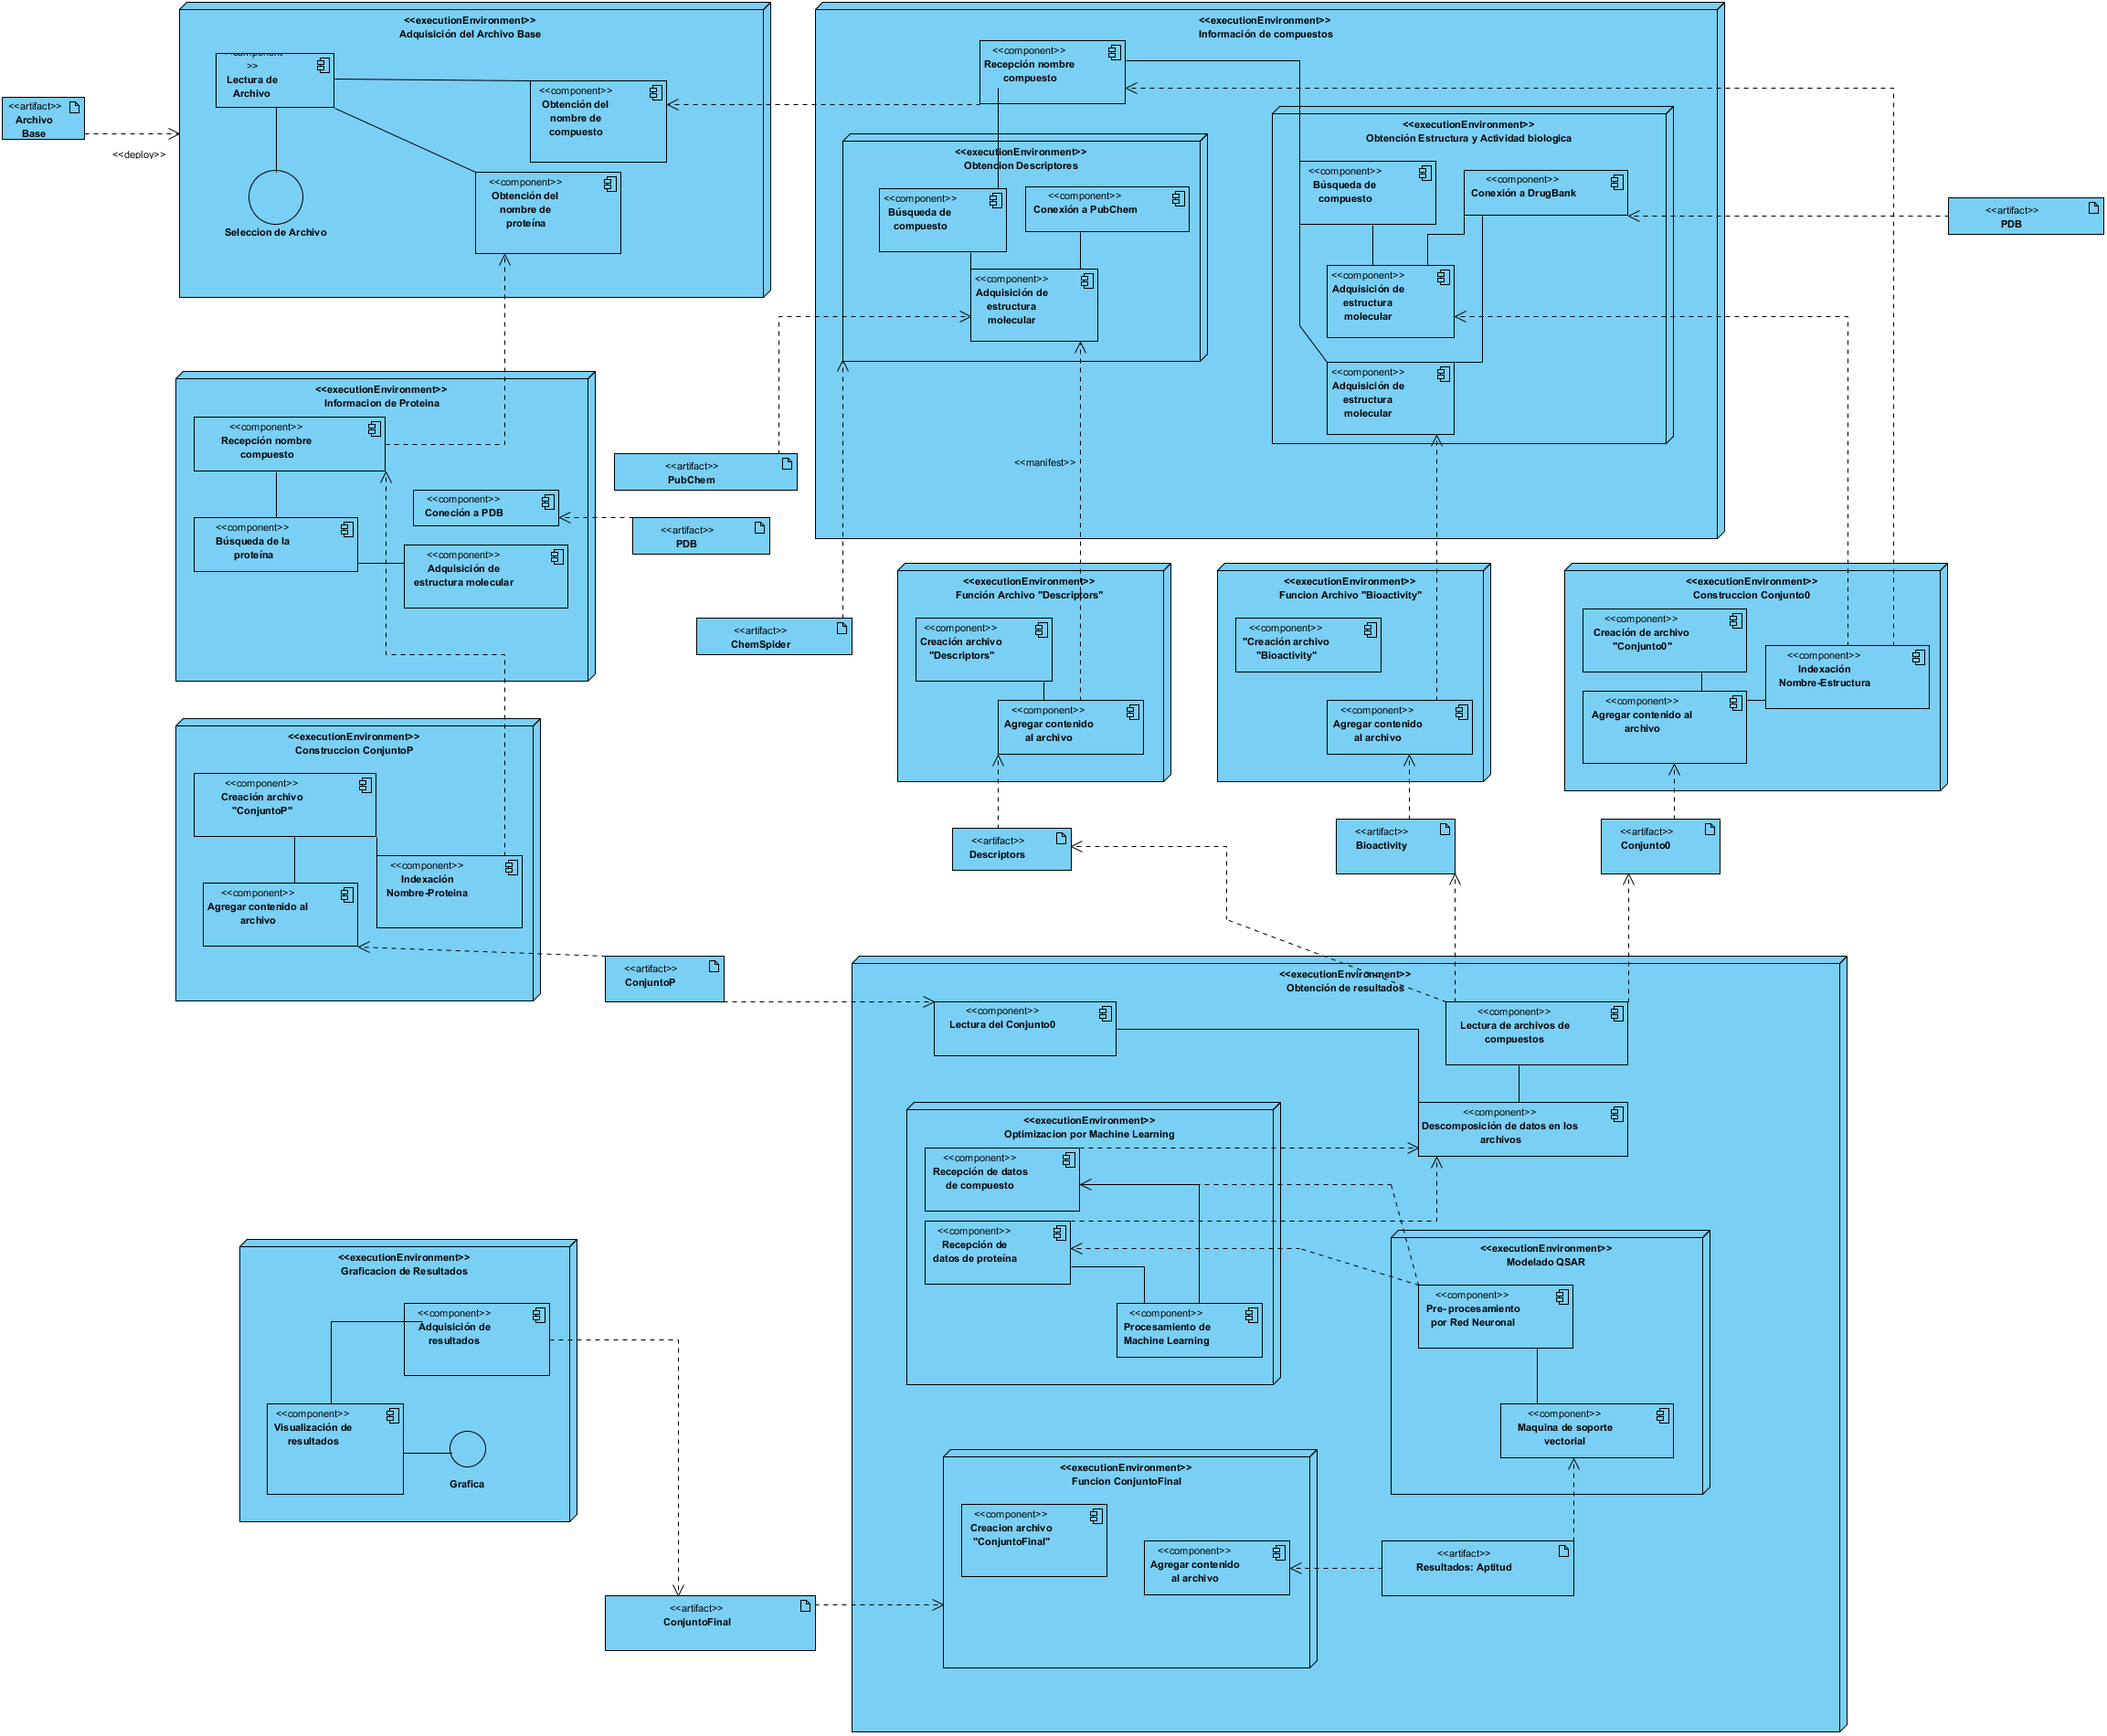
\includegraphics[scale=0.25]{Capitulo3/images/Niveles_de_Arquitectura.png}
    \caption{Niveles de Arquitectura}
    \label{arquitectura_N}
\end{figure}
\newpage

\section{Identificación de Requisitos de Diseño}
\noindent Se realiza la especificación de los requisitos que están directamente relacionados con la adopción o diseño de la arquitectura, y que pueden condicionar el diseño o la construcción del sistema de información.
% Please add the following required packages to your document preamble:
% \usepackage{multirow}
% \usepackage{longtable}
% Note: It may be necessary to compile the document several times to get a multi-page table to line up properly
\begin{longtable}{|l|l|l|l|}
\caption{Identificación de Requisitos de Diseño}
\label{req_dis}\\
\hline
\textbf{\begin{tabular}[c]{@{}l@{}}Módulo de \\ Arquitectura\end{tabular}}              & \textbf{\begin{tabular}[c]{@{}l@{}}Sub-Módulo de \\ Arquitectura\end{tabular}}                                                                                                                                                                                                  & \textbf{\begin{tabular}[c]{@{}l@{}}Requerimiento \\ Funcional\end{tabular}}                                                                 & \textbf{Descripción}                                                                                                                                                                                                                                                                                                                                           \\ \hline
\endfirsthead
%
\multicolumn{4}{c}%
{{\bfseries Tabla \thetable\ Continuación de la página anterior.}} \\
\endhead
%
\begin{tabular}[c]{@{}l@{}}Adquisición\\ de Archivo\\ Base\end{tabular}                 & \begin{tabular}[c]{@{}l@{}}- Lectura de\\ archivo\\ \\ - Selección de\\ archivo.\end{tabular}                                                                                                                                                                                   & \begin{tabular}[c]{@{}l@{}}Requerimiento\\ Funcional 1.1:\\ Obtención y\\ lectura del\\ archivo base.\end{tabular}                          & \begin{tabular}[c]{@{}l@{}}El sistema recibe del\\ usuario un archivo de\\ texto plano en el cual se\\ tiene una lista con los\\ nombres de los\\ compuestos y nombres\\ de las proteínas de la\\ patología que forman\\ parte del objeto de\\ estudio.\end{tabular}                                                                                           \\ 
\multirow{}{}{\begin{tabular}[c]{@{}l@{}}Información\\ de\\ compuestos.\end{tabular}} & \begin{tabular}[c]{@{}l@{}}- Recepción\\ nombre de\\ compuesto.\\ \\ - Obtención de\\ estructura y\\ actividad\\ biológica.\\ \\ - Conexión a\\ DrugBank.\\ \\ -Búsqueda del\\ compuesto.\\ \\ - Adquisición de\\ Estructura\\ molecular.\end{tabular}                          & \begin{tabular}[c]{@{}l@{}}Requerimiento\\ Funcional 1.2:\\ Búsqueda de\\ los compuestos\\ indicados.\end{tabular}                          & \begin{tabular}[c]{@{}l@{}}Por cada elemento de la\\ lista de compuestos en\\ el archivo ingresado por\\ el usuario, el sistema los\\ buscará en la base de\\ datos en línea\\ “DrugBank”.\end{tabular}                                                                                                                                                        \\ \cline{2-4} 
                                                                                        & \begin{tabular}[c]{@{}l@{}}- Recepción\\ nombre de\\ compuesto.\\ \\ - Obtención de\\ estructura y\\ actividad\\ biológica.\\ \\ - Conexión a\\ PubChem.\\ \\ - Conexión a\\ ChemSpider.\\ \\ - Búsqueda del\\ compuesto.\\ \\ -Adquisición de\\ los descriptores.\end{tabular} & \begin{tabular}[c]{@{}l@{}}Requerimiento\\ Funcional 1.3:\\ Búsqueda de\\ los descriptores\\ de los\\ compuestos.\end{tabular}              & \begin{tabular}[c]{@{}l@{}}El sistema, utilizando\\ como referencia la lista\\ de compuestos\\ ingresada por el usuario,\\ realiza una búsqueda de\\ los descriptores físico\\ químicos por cada uno\\ de los elementos de\\ dicha lista en la base de\\ datos “PubChem” y\\ ChemSpider.\end{tabular}                                                          \\ \cline{2-4} 
                                                                                        & \begin{tabular}[c]{@{}l@{}}- Recepción\\ nombre de\\ compuesto.\\ \\ - Obtención de\\ estructura y\\ actividad\\ biológica.\\ \\ - Conexión a\\ DrugBank.\\ \\ - Búsqueda del\\ compuesto.\\ \\ - Adquisición de la\\ actividad\\ biológica.\end{tabular}                       & \begin{tabular}[c]{@{}l@{}}Requerimiento\\ Funcional 1.4:\\ Búsqueda de\\ los mecanismos\\ de acción de los\\ compuestos.\end{tabular}      & \begin{tabular}[c]{@{}l@{}}El sistema, utilizando\\ como referencia la lista\\ de compuestos\\ ingresada por el usuario,\\ realiza la búsqueda de\\ los mecanismos de\\ acción por cada uno de\\ los elementos de dicha\\ lista en la base de datos\\ “DrugBank”.\end{tabular}                                                                                 \\ \hline
\begin{tabular}[c]{@{}l@{}}Información\\ de proteína.\end{tabular}                      & \begin{tabular}[c]{@{}l@{}}- Recepción\\ nombre proteína.\\ \\ - Conexión a PDB.\\ \\ - Búsqueda de la\\ proteína.\\ \\ - Adquisición de\\ estructura\\ molecular.\end{tabular}                                                                                                 & \begin{tabular}[c]{@{}l@{}}Requerimiento\\ Funcional 1.5:\\ Búsqueda de\\ las proteínas\\ indicadas.\end{tabular}                           & \begin{tabular}[c]{@{}l@{}}Por cada elemento de la\\ lista de proteínas en el\\ archivo ingresado por el\\ usuario, el sistema las\\ buscará en la base de\\ datos en línea “PDB”.\end{tabular}                                                                                                                                                                \\ \hline
\begin{tabular}[c]{@{}l@{}}Información\\ de Proteína.\end{tabular}                      & \begin{tabular}[c]{@{}l@{}}Adquisición de\\ estructura\\ molecular\\ proteína.\end{tabular}                                                                                                                                                                                     & \multirow{}{}{\begin{tabular}[c]{@{}l@{}}Requerimiento\\ Funcional 1.6:\\ Confirmación de\\ los resultados\\ de la búsqueda\end{tabular}} & \multirow{}{}{\begin{tabular}[c]{@{}l@{}}El sistema presenta al\\ usuario los resultados\\ de la búsqueda y este\\ último valida que sean\\ correctos.\end{tabular}}                                                                                                                                                                                         \\ \cline{1-2}
\begin{tabular}[c]{@{}l@{}}Información\\ de\\ Compuestos.\end{tabular}                  & \begin{tabular}[c]{@{}l@{}}- Adquisición de\\ estructura\\ molecular\\ compuesto\\ \\ \\ - Adquisición de\\ descriptores.\\ \\ \\ - Adquisición de\\ mecanismos de\\ acción.\end{tabular}                                                                                       &                                                                                                                                             &                                                                                                                                                                                                                                                                                                                                                                \\ \hline
\begin{tabular}[c]{@{}l@{}}Función\\ Archivo\\ “Descriptors”\end{tabular}               & \begin{tabular}[c]{@{}l@{}}- Creación archivo\\ descriptors.\\ \\ - Agregar\\ contenido al\\ archivo.\end{tabular}                                                                                                                                                              & \multirow{}{}{\begin{tabular}[c]{@{}l@{}}Requerimiento\\ Funcional 1.7:\\ Construcción de\\ conjuntos.\end{tabular}}                      & \multirow{}{}{\begin{tabular}[c]{@{}l@{}}El sistema organiza la\\ información recabada\\ durante el proceso de\\ búsqueda, en archivos\\ con estructuras\\ definidas, denominados\\ conjuntos, que permiten\\ continuar a la fase de\\ procesamiento de\\ información.\end{tabular}}                                                                         \\ \cline{1-2}
\begin{tabular}[c]{@{}l@{}}Función\\ Archivo\\ “BioActivity”\end{tabular}               & \begin{tabular}[c]{@{}l@{}}- Creación archivo\\ bioactivity.\\ \\ - Agregar\\ contenido al\\ archivo.\end{tabular}                                                                                                                                                              &                                                                                                                                             &                                                                                                                                                                                                                                                                                                                                                                \\ \hline
\begin{tabular}[c]{@{}l@{}}Construcción \\ Conjunto0\end{tabular}                       & \begin{tabular}[c]{@{}l@{}}- Creación archivo\\ Conjunto0.\\ \\ - Indexación\\ Nombre-Estructura.\\ \\ - Agregar\\ contenido al\\ archivo.\end{tabular}                                                                                                                         & \begin{tabular}[c]{@{}l@{}}Requerimiento\\ Funcional 1.7.1:\\ Construcción\\ del conjunto0\end{tabular}                                     & \begin{tabular}[c]{@{}l@{}}El sistema agrupa los\\ datos de los\\ compuestos (nombre,\\ estructura molecular,\\ mecanismos de acción)\\ en un conjunto de\\ archivos denominado\\ conjunto 0.\end{tabular}                                                                                                                                                     \\ \hline
\begin{tabular}[c]{@{}l@{}}Construcción \\ ConjuntoP\end{tabular}                       & \begin{tabular}[c]{@{}l@{}}- Creación archivo\\ Conjunto0.\\ \\ - Indexación\\ Nombre-Estructura.\\ \\ - Agregar\\ contenido al\\ archivo.\end{tabular}                                                                                                                         & \begin{tabular}[c]{@{}l@{}}Requerimiento\\ Funcional 1.7.2:\\ Construcción\\ del conjuntoP\end{tabular}                                     & \begin{tabular}[c]{@{}l@{}}El sistema agrupa la\\ información de la(s)\\ proteína(s) (nombre de\\ la proteína, estructura\\ molecular de la\\ proteína) de la patología\\ indicada por el usuario,\\ en un archivo\\ denominado conjunto P.\end{tabular}                                                                                                       \\ \hline
\multirow{4}{*}{\begin{tabular}[c]{@{}l@{}}Obtención\\ de\\ Resultados.\end{tabular}}   & \begin{tabular}[c]{@{}l@{}}- Lectura del\\ conjunto0\\ \\ - Descomposición\\ de archivo para\\ datos.\\ \\ - Recepción de\\ datos de\\ compuesto.\end{tabular}                                                                                                                  & \begin{tabular}[c]{@{}l@{}}Requerimiento\\ Funcional 2.1:\\ Adquisición y\\ descomposición\\ del conjunto0.\end{tabular}                    & \begin{tabular}[c]{@{}l@{}}El sistema lee el\\ conjunto 0 (previamente\\ definido)\\ correspondiente a un\\ compuesto, para\\ descomponerlo y \\ obtener nombre,\\ descriptores , estructura\\ molecular y mecanismos\\ de acción.\end{tabular}                                                                                                                \\ \cline{2-4} 
                                                                                        & \begin{tabular}[c]{@{}l@{}}- Lectura del\\ conjuntoP\\ \\ - Descomposición\\ de archivo para\\ datos.\\ \\ - Recepción de\\ datos de la\\ proteína.\end{tabular}                                                                                                                & \begin{tabular}[c]{@{}l@{}}Requerimiento \\ Funcional 2.2:\\ Adquisición y\\ descomposición\\ del conjuntoP.\end{tabular}                   & \begin{tabular}[c]{@{}l@{}}El sistema consigue el\\ nombre de la proteína\\ de interés así como su\\ estructura molecular\\ esta información\\ proveniente del conjunto P.\end{tabular}                                                                                                                                                                        \\ \cline{2-4} 
                                                                                        & \begin{tabular}[c]{@{}l@{}}Optimización\\ por Machine\\ Learning\end{tabular}                                                                                                                                                                                                   & \begin{tabular}[c]{@{}l@{}}Requerimiento\\ Funcional 2.3:\\ Método de\\ Machine\\ Learning\\  para\\ optimización.\end{tabular}             & \begin{tabular}[c]{@{}l@{}}El sistema,   a través de\\ este módulo trabaja  con\\ los datos\\ correspondientes al\\ compuesto  y proteína\\ con el objetivo de\\ optimizar la obtención\\ de resultados.\end{tabular}                                                                                                                                          \\ \cline{2-4} 
                                                                                        & \begin{tabular}[c]{@{}l@{}}- Modelado QSAR\\ \\ -Pre-procesamiento \\ por redes \\ neuronales\\ \\  - Maquina de\\ soporte vectorial\end{tabular}                                                                                                                               & \begin{tabular}[c]{@{}l@{}}Requerimiento\\ Funcional 2.4:\\ Modelado\\ QSAR.\end{tabular}                                                   & \begin{tabular}[c]{@{}l@{}}El sistema producirá\\ con los datos\\ pertenecientes a la\\ proteína y  compuesto\\ de interés  el modelo\\ QSAR propio de la\\ actividad farmacológica\\ entre el fármaco y la\\ proteína objetivo.\end{tabular}                                                                                                                  \\ \hline
\begin{tabular}[c]{@{}l@{}}Graficación\\ de\\ resultados.\end{tabular}                  & \begin{tabular}[c]{@{}l@{}}Adquisición de\\ resultados.\end{tabular}                                                                                                                                                                                                            & \begin{tabular}[c]{@{}l@{}}Requerimiento\\ Funcional 3.1:\\ Lectura y\\ ordenamiento\\ del conjunto\\ final.\end{tabular}                   & \begin{tabular}[c]{@{}l@{}}El sistema recibe el\\ conjunto final que\\ contiene el nombre del\\ compuesto y la  aptitud,\\ dicha información será\\ leída y ordena del más\\ apto al menos apto para\\ enfrentar la proteína de\\ la  patología indicada. A\\ la salida se tiene un\\ archivo de texto plano\\ que contiene una lista\\ ordenada.\end{tabular} \\ \hline
                                                                                        & \begin{tabular}[c]{@{}l@{}}Visualización de\\ resultados.\end{tabular}                                                                                                                                                                                                          & \begin{tabular}[c]{@{}l@{}}Requerimiento\\ Funcional 3.2:\\ Diseño gráfico\\ de resultados.\end{tabular}                                    & \begin{tabular}[c]{@{}l@{}}El sistema obtiene el\\ archivo que contiene la\\ lista ordenada  la cual\\ será utilizada para\\ desplegar de manera\\ gráfica  al usuario.\end{tabular}                                                                                                                                                                           \\ \hline
\end{longtable}

\newpage
%%%%%%%%%%%%%%%%%%%%%%%%%%%%%%%%%%%%%%%%%5
\section{Especificación de Excepciones}
\noindent El objetivo de esta tarea es la definición de los comportamientos no habituales en el
sistema, que reflejan situaciones anómalas o secundarias en el funcionamiento y ejecución del
sistema de información. Para ello, se establece previamente el nivel de especificación de las
mismas, así como los criterios de catalogación y clasificación.
Se propone su catalogación como ayuda para el diseño del sistema de información y
como guía en la especificación técnica de las pruebas, al permitir la generación de algunos
casos de prueba de forma inmediata. Dicho catálogo se va completando a partir de las
actividades correspondientes al diseño detallado de los subsistemas.\\

Las excepciones se describen incluyendo, al menos, los siguientes conceptos:\\

\begin{itemize}
    \item Tipo y descripción de la excepción.
    \item Condiciones previas del sistema de información.
    \item Elemento afectado (nodo, módulo, caso de uso).
    \item Respuesta del sistema de información.
    \item Elemento asociado a la respuesta esperada del sistema (módulo, clase, procedimiento,etc.).
\end{itemize}

%%%%%%%%%%%%%%%%%%%%%%%%%%%%%%%%%5
% Please add the following required packages to your document preamble:
% \usepackage{longtable}
% Note: It may be necessary to compile the document several times to get a multi-page table to line up properly
\begin{longtable}{|l|l|l|l|l|}
\caption{Catalogo de Excepciones}
\label{catalogo_de_excepciones}\\
\hline
\textbf{ID} & \textbf{\begin{tabular}[c]{@{}l@{}}Nombre de\\ Excepción\end{tabular}}                        & \textbf{Descripción}                                                                                                                                                                                                                                                           & \textbf{\begin{tabular}[c]{@{}l@{}}Ubicación\\ (Requerimiento)\end{tabular}}                                      & \textbf{\begin{tabular}[c]{@{}l@{}}Elemento\\ afectado\end{tabular}} \\ \hline
\endfirsthead
%
\multicolumn{5}{c}%
{{\bfseries Tabla \thetable\ Continuación de la página anterior}} \\
\endhead
%
EX1         & \begin{tabular}[c]{@{}l@{}}Excepción  \\ lectura del \\ archivo base.\end{tabular}            & \begin{tabular}[c]{@{}l@{}}Excepción que se \\ genera al \\ presentarse \\ un error de en \\ adquisición del \\ archivo base:\\ - No se encuentra \\ el archivo.\\ - El archivo está \\ corrompido o \\ incompleto.\end{tabular}                                               & \begin{tabular}[c]{@{}l@{}}RF1.1: \\ Obtención \\ y lectura del \\ archivo base.\end{tabular}                     & \begin{tabular}[c]{@{}l@{}}Archivo \\ base.\end{tabular}             \\ \hline
EX2         & \begin{tabular}[c]{@{}l@{}}Excepción de \\ formato de \\ datos.\end{tabular}                  & \begin{tabular}[c]{@{}l@{}}Excepción de error \\ de los datos \\ existentes en\\ el archivo base.\\ - No es posible la\\ adquisición del \\ nombre de \\ compuesto o\\ proteína.\\ - El  dato adquirido \\ no tiene sentido \\ con lo que debe de \\ representar.\end{tabular} & \begin{tabular}[c]{@{}l@{}}RF1.1: \\ Obtención y\\ lectura del \\ archivo base.\end{tabular}                      & \begin{tabular}[c]{@{}l@{}}Nombre \\ del\\ compuesto.\end{tabular}   \\ \hline
EX3         & \begin{tabular}[c]{@{}l@{}}Excepción de\\ conexión a\\ DrugBank\end{tabular}                  & \begin{tabular}[c]{@{}l@{}}Excepción que \\ indica error en \\ la conexión a\\ las bases de datos.\\ - Error de conexión\\  a DrugBank\end{tabular}                                                                                                                            & \begin{tabular}[c]{@{}l@{}}RF1.2: \\ Búsqueda de\\ los compuestos\\ indicados.\end{tabular}                       & \begin{tabular}[c]{@{}l@{}}Archivo\\ “Conjunto0”\end{tabular}        \\ \hline
EX4         & \begin{tabular}[c]{@{}l@{}}Excepción\\ Compuesto no\\ encontrado.\end{tabular}                & \begin{tabular}[c]{@{}l@{}}Excepción que \\ notifica que no \\ existe el\\ compuesto en\\ DrugBank.\\ - Error\\ compuesto\\ inexistente.\end{tabular}                                                                                                                          & \begin{tabular}[c]{@{}l@{}}RF1.2: \\ Búsqueda de\\ los compuestos\\ indicados.\end{tabular}                       & \begin{tabular}[c]{@{}l@{}}Archivo\\ “Conjunto0”\end{tabular}        \\ \hline
EX5         & \begin{tabular}[c]{@{}l@{}}Excepción no se \\ puede obtener \\ datos.\end{tabular}            & \begin{tabular}[c]{@{}l@{}}Excepción que \\ indica que no \\ se pudo adquirir\\ información.\\ - Error de \\ adquisición\end{tabular}                                                                                                                                          & \begin{tabular}[c]{@{}l@{}}RF1.2: \\ Búsqueda de\\ los compuestos\\ indicados.\end{tabular}                       & \begin{tabular}[c]{@{}l@{}}Archivo\\ “Conjunto0”\end{tabular}        \\ \hline
EX6         & \begin{tabular}[c]{@{}l@{}}Excepción de \\ conexión a \\ PubChem\end{tabular}                 & \begin{tabular}[c]{@{}l@{}}Excepción que \\ indica error en \\ la conexión a\\ las bases de datos.\\ - Error de conexión\\ a PubChem\end{tabular}                                                                                                                              & \begin{tabular}[c]{@{}l@{}}RF1.3: \\ Búsqueda de \\ los descriptores \\ de los \\ compuestos.\end{tabular}        & \begin{tabular}[c]{@{}l@{}}Archivo \\ “Descriptors”\end{tabular}     \\ \hline
EX7         & \begin{tabular}[c]{@{}l@{}}Excepción \\ Compuesto \\ no encontrado.\end{tabular}              & \begin{tabular}[c]{@{}l@{}}Excepción que\\ notifica que no \\ existe el \\ compuesto en \\ DrugBank.\\ - Error compuesto \\ inexistente.\end{tabular}                                                                                                                          & \begin{tabular}[c]{@{}l@{}}RF1.3: \\ Búsqueda de \\ los descriptores \\ de los \\ compuestos.\end{tabular}        & \begin{tabular}[c]{@{}l@{}}Archivo \\ “Descriptors”\end{tabular}     \\ \hline
EX8         & \begin{tabular}[c]{@{}l@{}}Excepción no \\ se puede \\ obtener datos.\end{tabular}            & \begin{tabular}[c]{@{}l@{}}Excepción que \\ indica que no \\ se pudo adquirir \\ información.\\ - Error de \\ adquisición\end{tabular}                                                                                                                                         & \begin{tabular}[c]{@{}l@{}}RF1.3: \\ Búsqueda de \\ los descriptores \\ de los \\ compuestos.\end{tabular}        & \begin{tabular}[c]{@{}l@{}}Archivo \\ “Descriptors”\end{tabular}     \\ \hline
EX9         & \begin{tabular}[c]{@{}l@{}}Excepción no \\ se puede obtener \\ datos.\end{tabular}            & \begin{tabular}[c]{@{}l@{}}Excepción que \\ indica que no \\ se pudo adquirir \\ información.\\ - Error de \\ adquisición\end{tabular}                                                                                                                                         & \begin{tabular}[c]{@{}l@{}}RF1.4: \\ Búsqueda de \\ los mecanismos\\ de acción de los \\ compuestos.\end{tabular} & \begin{tabular}[c]{@{}l@{}}Archivo \\ “BioAcitvity”\end{tabular}     \\ \hline
EX10        & \begin{tabular}[c]{@{}l@{}}Excepción de \\ conexión a PDB\end{tabular}                        & \begin{tabular}[c]{@{}l@{}}Excepción que \\ indica error en \\ la conexión a \\ las bases de datos.\\ - Error de conexión \\ a PDB\end{tabular}                                                                                                                                & \begin{tabular}[c]{@{}l@{}}RF1.5: \\ Búsqueda de\\ las proteínas \\ indicadas.\end{tabular}                       & \begin{tabular}[c]{@{}l@{}}Archivo \\ “ConjuntoP”\end{tabular}       \\ \hline
EX11        & \begin{tabular}[c]{@{}l@{}}Excepción \\ Compuesto no\\ encontrado.\end{tabular}               & \begin{tabular}[c]{@{}l@{}}Excepción que \\ notifica que no \\ existe la proteína \\ en PDB.\\ - Error compuesto \\ inexistente.\end{tabular}                                                                                                                                  & \begin{tabular}[c]{@{}l@{}}RF1.5: \\ Búsqueda de\\ las proteínas \\ indicadas.\end{tabular}                       & \begin{tabular}[c]{@{}l@{}}Archivo \\ “ConjuntoP”\end{tabular}       \\ \hline
EX12        & \begin{tabular}[c]{@{}l@{}}Excepción no se \\ puede obtener \\ datos.\end{tabular}            & \begin{tabular}[c]{@{}l@{}}Excepción que \\ indica que no \\ se pudo adquirir \\ información.\\ - Error de \\ adquisición\end{tabular}                                                                                                                                         & \begin{tabular}[c]{@{}l@{}}RF1.5: \\ Búsqueda de\\ las proteínas \\ indicadas.\end{tabular}                       & \begin{tabular}[c]{@{}l@{}}Archivo \\ “ConjuntoP”\end{tabular}       \\ \hline
EX13        & \begin{tabular}[c]{@{}l@{}}Excepción de \\ archivo \\ conjunto0\end{tabular}                  & \begin{tabular}[c]{@{}l@{}}Excepción que \\ notifica error  de \\ creación del \\ conjunto0.\\ - Error de creación \\ de archivo\end{tabular}                                                                                                                                  & \begin{tabular}[c]{@{}l@{}}RF1.7.1: \\ Construcción\\ del conjunto cero.\end{tabular}                             & \begin{tabular}[c]{@{}l@{}}Archivo \\ “Conjunto0”\end{tabular}       \\ \hline
EX14        & \begin{tabular}[c]{@{}l@{}}Excepción de \\ archivo \\ conjuntoP\end{tabular}                  & \begin{tabular}[c]{@{}l@{}}Excepción que \\ notifica error  de \\ creación del \\ conjuntoP.\\ - Error de creación \\ de archivo.\end{tabular}                                                                                                                                 & \begin{tabular}[c]{@{}l@{}}RF1.7.2 : \\ Construcción \\ del conjunto P.\end{tabular}                              & \begin{tabular}[c]{@{}l@{}}Archivo \\ “ConjuntoP”\end{tabular}       \\ \hline
EX15        & \begin{tabular}[c]{@{}l@{}}Excepción  \\ lectura del \\ archivo \\ Conjunto0\\ .\end{tabular} & \begin{tabular}[c]{@{}l@{}}Excepción que se \\ genera al no poder \\ leer el archivo \\ Conjunto0:\\ - No se encuentra \\ el archivo.\\ - El archivo está \\ corrompido o \\ incompleto.\end{tabular}                                                                          & \begin{tabular}[c]{@{}l@{}}RF2.1: \\ Adquisición y\\ descomposición \\ del Conjunto0.\end{tabular}                & \begin{tabular}[c]{@{}l@{}}Archivo \\ “Conjunto0”\end{tabular}       \\ \hline
EX16        & \begin{tabular}[c]{@{}l@{}}Excepción  \\ lectura del \\ archivo \\ ConjuntoP.\end{tabular}    & \begin{tabular}[c]{@{}l@{}}Excepción que se \\ genera al no poder \\ leer el archivo \\ ConjuntoP:\\ - No se encuentra \\ el archivo.\\ - El archivo está \\ corrompido o \\ incompleto.\end{tabular}                                                                          & \begin{tabular}[c]{@{}l@{}}RF2.2: \\ Adquisición y \\ descomposición \\ del ConjuntoP\\ .\end{tabular}            & \begin{tabular}[c]{@{}l@{}}Archivo \\ “ConjuntoP”\end{tabular}       \\ \hline
\end{longtable}
\section{Especificación de Estándares y Normas de
Diseño y Construcción}
\noindent En esta sección se definen los estándares técnicos y de nomenclatura, normas y
recomendaciones, que generalmente están relacionados con la adopción o diseño de una arquitectura o infraestructura tecnológica concreta, y que pueden condicionar el diseño o la construcción del sistema de información.
% Please add the following required packages to your document preamble:
% \usepackage{longtable}
% Note: It may be necessary to compile the document several times to get a multi-page table to line up properly
\begin{longtable}{|l|p{3.7cm}|p{4cm}|p{4.7cm}|}
\caption{Especificación de Estándares y Normas de Diseño y Construcción}
\label{estandares}\\
\hline
\textbf{Norma}                                      & \textbf{Descripción}                                                                                                                                                                                                                                                                                                                                                                                        & \textbf{Tareas (Métricas)}                                                                                                                                                                                                                                                         & \textbf{Aplicación al sistema}                                                                                                                                                                                                                                                                                                                                                                                                                                                                                                                                    \\ \hline
\endfirsthead
%
\multicolumn{4}{c}%
{{\bfseries Tabla \thetable\ Continuación de la página anterior}} \\
\endhead
%
\begin{tabular}[c]{@{}l@{}}ISO \\ 9126\end{tabular} & \begin{tabular}[c]{@{}l@{}}El estándar ISO\\ 9126 ha sido\\ desarrollado en un\\ intento de identificar\\ los atributos clave\\ de calidad para el\\ software evalúa los\\ productos de\\ software, esta\\ norma nos indica\\ las características\\ de la calidad y los\\ lineamientos para\\ su uso. El estándar\\ identifica 6 atributos\\ clave de calidad.\end{tabular}                                 & \begin{tabular}[c]{@{}l@{}}Funcionalidad: El\\ grado en que el\\ software satisface las\\ necesidades indicadas\\ por los siguientes\\ subatributos:\\ idoneidad, corrección,\\ interoperatividad,\\ conformidad y\\ seguridad.\end{tabular}                                       & \begin{tabular}[c]{@{}l@{}}- Adquisición del \\archivo base. \\ - Conexión a las bases\\ de datos.\\ - Obtención de los datos \\del compuesto.\\  - Obtención de los datos \\del compuesto.\\  - Correcta creación de \\los archivos contenedores\\ de datos del compuesto.\\  - Correcta creación de los\\ archivos contenedores de \\datos del compuesto.\\  - Lectura de los datos\\ perteneciente a compuestos.\\  - Lectura de los datos\\ perteneciente a la proteína.\\  - Obtención de\\ resultados.\end{tabular} \\ \hline
\begin{tabular}[c]{@{}l@{}}ISO \\ 9126\end{tabular} &                                                                                                                                                                                                                                                                                                                                                                                                             & \begin{tabular}[c]{@{}l@{}}Confiabilidad:\\ Cantidad de tiempo\\ que el software está\\ disponible para su\\ uso. Está referido por\\ los siguientes\\ subatributos: madurez,\\ tolerancia a fallos y\\ facilidad de\\ recuperación.\end{tabular}                                  & \begin{tabular}[c]{@{}l@{}}- Adquisición de los los \\datos de los compuestos.\\- Adquisición de  los datos \\de  la(s) proteína(s).\\- Conexión a las bases de \\datos (PubChem, \\DrugBank, \\ PDB).\\- Generación de resultados.\end{tabular}                                                                                                                                                                                                                                                                                 \\ \hline
\begin{tabular}[c]{@{}l@{}}ISO \\ 9126\end{tabular} &                                                                                                                                                                                                                                                                                                                                                                                                             & \begin{tabular}[c]{@{}l@{}}Usabilidad: Grado en\\ que el software es fácil\\ de usar. Viene\\ reflejado por los\\ siguientes\\ subatributos: facilidad\\ de comprensión,\\ facilidad de\\ aprendizaje y\\ operatividad.\end{tabular}                                               & \begin{tabular}[c]{@{}l@{}}- Interfaces.\\- Adquisición  del archivo \\base.\\- El usuario únicamente \\ debe cargar con  la \\estructura adecuada el \\“ArchivoBase”\end{tabular}                                                                                                                                                                                                                                                                                                                                                                        \\ \hline
\begin{tabular}[c]{@{}l@{}}ISO \\ 9126\end{tabular} &                                                                                                                                                                                                                                                                                                                                                                                                             & \begin{tabular}[c]{@{}l@{}}Eficiencia: Grado en\\ que el software hace\\ óptimo el uso de los\\ recursos del sistema.\\ Está indicado por los\\ siguientes\\ subatributos: tiempo\\ de uso y recursos\\ utilizados.\end{tabular}                                                   & \begin{tabular}[c]{@{}l@{}}- Ponderación asignada \\en el plan de pruebas.\\- Obtención de Resultados.\end{tabular}                                                                                                                                                                                                                                                                                                                                                                                                                               \\ \hline
\begin{tabular}[c]{@{}l@{}}ISO \\ 9126\end{tabular} &                                                                                                                                                                                                                                                                                                                                                                                                             & \begin{tabular}[c]{@{}l@{}}Facilidad de\\ mantenimiento: La\\ facilidad con que una\\ modificación puede\\ ser realizada. Está\\ indicada por los\\ siguientes\\ subatributos: facilidad\\ de análisis, facilidad\\ de cambio, estabilidad\\ y facilidad de prueba.\end{tabular}   & \begin{tabular}[c]{@{}l@{}}- El sistema ha sido \\ dividido en módulos  y \\submódulos permitiendo\\ de ser necesario, el \\ mantenimiento unitario \\y por integración de ellos.\end{tabular}                                                                                                                                                                                                                                                                                                                                                             \\ \hline
\begin{tabular}[c]{@{}l@{}}ISO \\ 9126\end{tabular} &                                                                                                                                                                                                                                                                                                                                                                                                             & \begin{tabular}[c]{@{}l@{}}Portabilidad: La\\ facilidad con que el\\ software puede ser\\ llevado de un entorno\\ a otro. Está referido\\ por los siguientes\\ subatributos: facilidad\\ de instalación,\\ facilidad de ajuste,\\ facilidad de\\ adaptación al cambio\end{tabular} & - TBD(Por definirse)                                                                                                                                                                                                                                                                                                                                                                                                                                                                                                                                               \\ \hline
\begin{tabular}[c]{@{}l@{}}ISO \\ 9241\end{tabular} & \begin{tabular}[c]{@{}l@{}}ISO 9241-210:2010\\ constituye un marco\\ de trabajo para  el\\ diseño  centrado  en\\ las  personas  al\\ integrar diferentes\\ procesos de diseño y\\ desarrollo apropiados\\ a un  contexto  en\\ particular;\\ complementando  las\\ metodologías de\\ diseño  existentes.\\ Para evaluar las\\ interfaces, esta se\\ centra en 6\\ actividades\\ primordiales.\end{tabular} & \begin{tabular}[c]{@{}l@{}}Consistencia: \\ La apariencia de toda \\la interfaz debe ser\\ consistente con los\\ estándares de la\\ industria del software.\end{tabular}                                                                                                           & \begin{tabular}[c]{@{}l@{}}El sistema cuenta con la\\ misma topología de\\ letras, tamaño, colores\\ que se usan e imágenes\\ lo cual lo hace constante.\end{tabular}                                                                                                                                                                                                                                                                                                                                                                                            \\ \hline
\begin{tabular}[c]{@{}l@{}}ISO \\ 9241\end{tabular} &                                                                                                                                                                                                                                                                                                                                                                                                             & \begin{tabular}[c]{@{}l@{}}Facilidad de uso:\\ Deben proporcionarse\\ “atajos” de teclado\\ para los usuarios más\\ experimentados.\end{tabular}                                                                                                                                   & \begin{tabular}[c]{@{}l@{}}El sistema implementa\\ atajos para cargar el\\ archivo con mayor\\ rapidez.\end{tabular}                                                                                                                                                                                                                                                                                                                                                                                                                                               \\ \hline
\begin{tabular}[c]{@{}l@{}}ISO \\ 9241\end{tabular} &                                                                                                                                                                                                                                                                                                                                                                                                             & \begin{tabular}[c]{@{}l@{}}Reducción de la\\ confusión: Debe\\ evitarse la confusión al\\ usuario inexperto por\\ la presentación de\\ excesivas opciones.\end{tabular}                                                                                                            & \begin{tabular}[c]{@{}l@{}}El sistema es bastante\\ claro con cada uno de\\ los botones que\\ proporciona, ya que su\\ función se encuentra en\\ la descripción del\\ mismo.\end{tabular}                                                                                                                                                                                                                                                                                                                                                                          \\ \hline
\begin{tabular}[c]{@{}l@{}}ISO \\ 9241\end{tabular} &                                                                                                                                                                                                                                                                                                                                                                                                             & \begin{tabular}[c]{@{}l@{}}Mensajes al usuario:\\ Los mensajes deben\\ ser claros y útiles. Por\\ ejemplo, en el caso de\\ los mensajes de error,\\ este error debe poder\\ ser corregido con la\\ información\\ proporcionada en el\\ mensaje de aviso.\end{tabular}              & \begin{tabular}[c]{@{}l@{}}Los mensajes que son\\ mostrados al usuario,\\ son claros en cuanto a\\ la excepción que se\\ generó.\end{tabular}                                                                                                                                                                                                                                                                                                                                                                                                                      \\ \hline
\begin{tabular}[c]{@{}l@{}}ISO \\ 9241\end{tabular} &                                                                                                                                                                                                                                                                                                                                                                                                             & \begin{tabular}[c]{@{}l@{}}Iconos: Debe\\ asegurarse que la\\ interfaz proporciona\\ un feedback al usuario\\ apropiado, necesario y\\ consistente.\end{tabular}                                                                                                                   & \begin{tabular}[c]{@{}l@{}}No existen iconos que\\ contengan juegos de\\ palabras o nombres\\ de aplicaciones por lo\\ cual los iconos y sus\\ usos son claros.\end{tabular}                                                                                                                                                                                                                                                                                                                                                                                       \\ \hline
\begin{tabular}[c]{@{}l@{}}ISO \\ 9241\end{tabular} &                                                                                                                                                                                                                                                                                                                                                                                                             & \begin{tabular}[c]{@{}l@{}}Sistemas de ayuda: La\\ ayuda proporcionada\\ debe estar disponible\end{tabular}                                                                                                                                                                        & \begin{tabular}[c]{@{}l@{}}El sistema cuenta con\\ un apartado de ayuda\\ donde el usuario podrá\\ ponerse en contacto a\\ través de correo\\ electrónico para atender\\ sus inquietudes.\end{tabular}                                                                                                                                                                                                                                                                                                                                                             \\ \hline
\end{longtable}


%%%%%%%%%%%%%%%%%%%%%%%%%%%%%%%%%%%%%
\section{Identificación de Subsistemas de Diseño}
\noindent En este apartado se divide de forma lógica el sistema de información en subsistemas de
diseño, con el fin de reducir la complejidad y facilitar el mantenimiento. Hay que tomar como
referencia inicial los subsistemas de análisis especificados en el proceso de Análisis del
Sistema de Información (ASI).
\subsection{Diagramas de estructura}

\begin{figure}[H]
    \centering
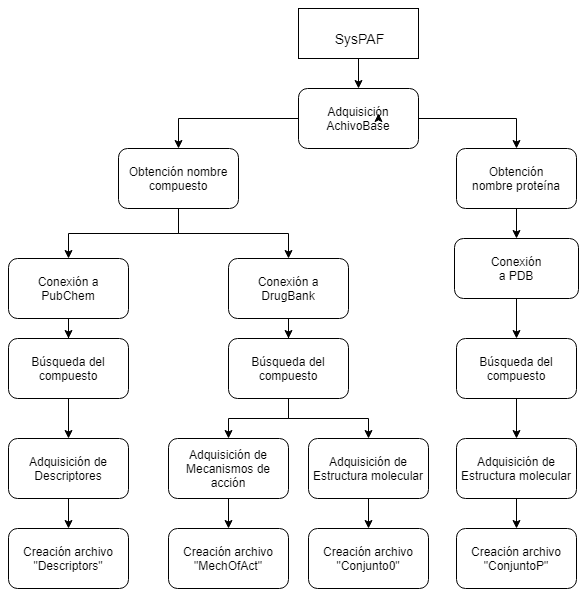
\includegraphics[scale=0.5]{Capitulo3/images/1_5Estructura.png}
    \caption{Diagrama de Estructura}
    \label{Diagramas_de_estructura}
\end{figure}

\begin{figure}[H]
    \centering
    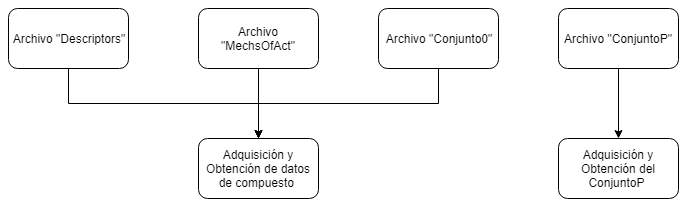
\includegraphics[scale=0.5]{Capitulo3/images/1_5EstructuraMod2.png}
    \caption{Diagrama de Estructura modulo 2}
    \label{Diagrama_Estruct_mod2}
\end{figure}
%%%%%%%%%%%%%%%%%%%%%%%%%%%%%%%5
\section{Especificación de requisitos de operación y seguridad}
\noindent El objetivo de esta tarea es definir los procedimientos de seguridad y operación
necesarios para no comprometer el correcto funcionamiento del sistema y garantizar el
cumplimiento de los niveles de servicios que exigirá el sistema en cuanto a la gestión de
operaciones (procesos por lotes, seguridad, comunicaciones, etc.).
% Please add the following required packages to your document preamble:
% \usepackage{longtable}
% Note: It may be necessary to compile the document several times to get a multi-page table to line up properly
\begin{longtable}{|l|l|l|}
\caption{Especificación de requisitos de operación y seguridad}
\label{Especificacion_de_req_op_seg}\\
\hline
\textbf{ID Requerimiento} & \textbf{Nombre}              & \textbf{Descripción}                                                                                                                                                                                                                                                    \\ \hline
\endfirsthead
%
\multicolumn{3}{c}%
{{\bfseries Tabla \thetable\ Continuación de la página anterior}} \\
\endhead
%
RFS1                      & Control de modificaciones.   & \begin{tabular}[c]{@{}l@{}}Se debe generar una\\ bitácora de la tarea a \\ realizar indicando:\\ - Actividad realizada.\\ - Indicación de módulo\\ de proceso modificado.\\ - Miembro que lo realizó.\end{tabular}                                                      \\ \hline
RFS2                      & Revisión de versiones.       & \begin{tabular}[c]{@{}l@{}}A través de la herramienta \\ Git, logrando llevar a cabo \\ un seguimiento del \\ versionado del sistema.\end{tabular}                                                                                                                      \\ \hline
RFS3                      & Acceso a Archivo             & \begin{tabular}[c]{@{}l@{}}Garantizar, que si el usuario\\ desea ver la información\\ existente en los archivos, \\ sea solo vista.\end{tabular}                                                                                                                        \\ \hline
RFS4                      & Negación de modificación     & \begin{tabular}[c]{@{}l@{}}Se debe de garantizar, que\\ los archivos donde se\\ almacene la información \\ obtenida, sea solo \\ modificada por el sistema.\end{tabular}                                                                                                \\ \hline
RFS5                      & Modificación al sistema      & \begin{tabular}[c]{@{}l@{}}El usuario, no tendrá la \\ capacidad de modificar o\\ alterar configuraciones \\ del sistema, más que \\ aspectos de visualización \\ e interfaz gráfica.\end{tabular}                                                                      \\ \hline
RFS6                      & Acceso a las bases de datos. & \begin{tabular}[c]{@{}l@{}}No habrá manera en la\\ que se modifique el \\ acceso a las bases de \\ datos para la recolección \\ de información.\\ - Cambios en la \\ dirección de la \\ base de datos.\\ - Alteración en el \\ driver para la \\ conexión.\end{tabular} \\ \hline
\end{longtable}
\section{Verificación de las Especificaciones de Diseño}
\noindent El objetivo de esta tarea es asegurar la calidad formal de los distintos modelos, conforme
a la técnica seguida para la elaboración de cada producto y a las normas y estándares
especificados en el catálogo de normas.

\begin{figure}[H]
    \centering
    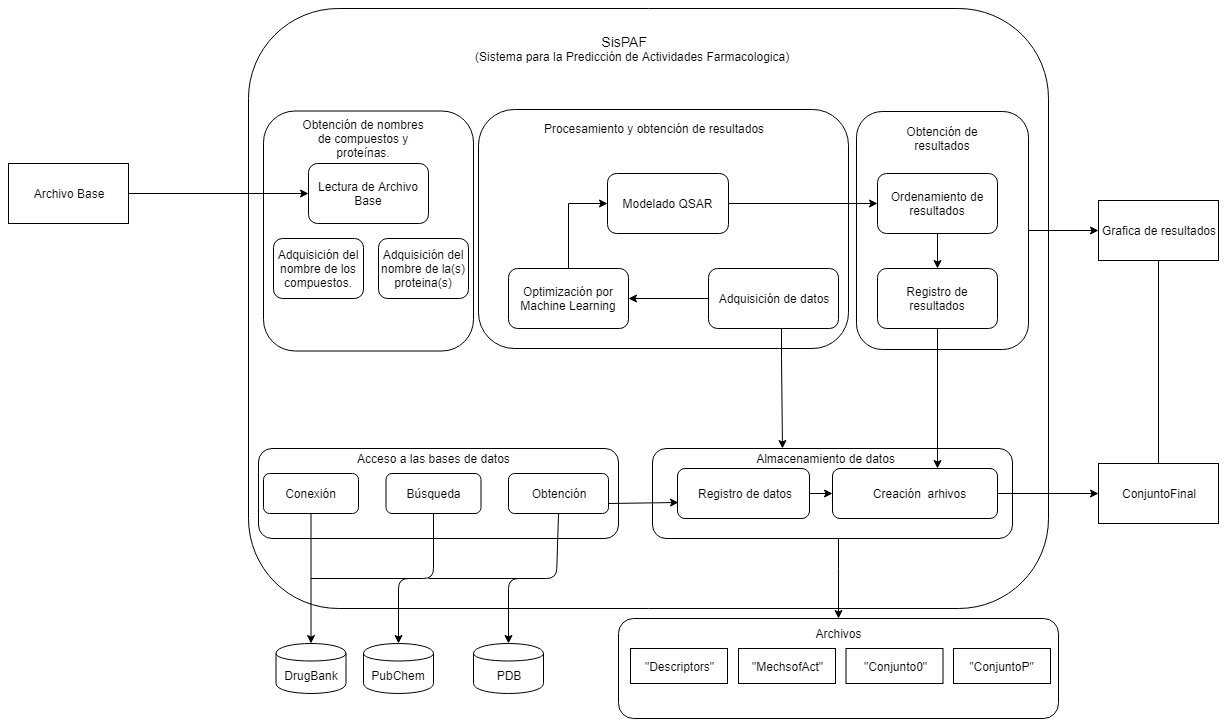
\includegraphics[scale=0.35]{Capitulo3/images/7_1.png}
    \caption{Diseño de arquitectura modular.}
    \label{Diagram_4}
\end{figure}
 %Obligatorio
\lhead{Capítulo \ref{ch_5}}
\rhead{\newtitle}
\cfoot{\thepage}
\renewcommand{\headrulewidth}{1pt}
\renewcommand{\footrulewidth}{1pt}

\chapter{Construcción del Sistema de Información}\label{ch_5}
\noindent En este proceso se genera el código de los componentes del Sistema de Información, se desarrollan todos los procedimientos de operación y seguridad y se elaboran todos los manuales de usuario final con el objetivo de asegurar el correcto funcionamiento del Sistema para su posterior implantación.\\

\noindent Para conseguir dicho objetivo, en este proceso se realizan las pruebas unitarias, las pruebas de integración de los subsistemas y componentes y las pruebas del sistema, de acuerdo al plan de pruebas establecido.
\newpage
%% ---------- Preparación del entorno -------------- %%
\section{Preparación del Entorno de Construcción}{
\noindent La preparación del entorno de construcción implica la descripción de los puestos de trabajo y la instalación de las herramientas y bibliotecas a usar durante el desarrollo y codificación del proyecto.\\

\noindent Como consideración previa se contempla que las computadoras usadas para el desarrollo deben de poseer el sistema operativo GNU/Linux, específicamente en su distribución Ubuntu.

\subsection{Puestos de trabajo}{
\noindent Para los puestos de trabajo se tiene contemplado hacer uso de 3 computadoras portátiles (1 para cada miembro del equipo de trabajo) las cuales cumplan con lo necesario para poder instalar y hacer uso de las diferentes herramientas y librerías que se especifican en los apartados X y Z respectivamente. Los equipos que con los que actualmente se cuenta son los siguientes:
% Please add the following required packages to your document preamble:
% \usepackage{longtable}
% Note: It may be necessary to compile the document several times to get a multi-page table to line up properly
\begin{longtable}[c]{lllll}
\cline{1-2}
\multicolumn{1}{|l|}{\textbf{Equipo}}           & \multicolumn{1}{l|}{\textbf{Especificaciones Técnicas}}                                                                                                                                                                                                                                    &  &  &  \\ \cline{1-2}
\endfirsthead
%
\multicolumn{5}{c}%
{{\bfseries Table \thetable\ continued from previous page}} \\
\endhead
%
\multicolumn{1}{|l|}{HP Notebook - 15-ac128la}  & \multicolumn{1}{l|}{\begin{tabular}[c]{@{}l@{}}°Procesador Intel Core i7-6500U (2,5 GHz,\\     hasta 3,1 GHz, 4 MB de caché, 2 núcleos).\\ Memoria RAM de 8GB\\ Gráficos de video Intel HD 520\\ Disco Duro SATA de 2TB 5400 rpm\end{tabular}}                                          &  &  &  \\ \cline{1-2}
\multicolumn{1}{|l|}{HP Pavilion Laptop 15-cw0} & \multicolumn{1}{l|}{\begin{tabular}[c]{@{}l@{}}Procesador AMD Ryzen 3 con \\    gráficos Radeon Vega Graphics \\    Mobile Gfx (Cuatro núcleos a 3,4 GHz \\    en modo base y 3,7 GHz en modo turbo).\\ Memoria RAM de 12GB.\\ Disco Duro SSD SATA3 de 500 GB.\end{tabular}}           &  &  &  \\ \cline{1-2}
\multicolumn{1}{|l|}{Lenovo Ideapad 110-14 ISK} & \multicolumn{1}{l|}{\begin{tabular}[c]{@{}l@{}}°Procesador Intel Core i7-649DU (2,5 GHz, \\   hasta 3,1 GHz, 4 MB de caché, 4 núcleos).\\ Memoria RAM de 8GB .Disco Duro Toshiba\\    MQ01 de 1TB.Disco Duro Kingston SSD \\    de 240 GB.\\ °Gráficos de video Intel HD510\end{tabular}} &  &  &  \\ \cline{1-2}
                                                &                                                                                                                                                                                                                                                                                            &  &  & 
\end{longtable}
}
\subsection{Herramientas}{
\subsubsection{Visual Studio Code}

\noindent Visual Studio Code es un editor de código fuente desarrollado por \textbf{Microsoft} y este puede ser utilizado en los Sistemas Operativos \textbf{Linux}, \textbf{macOS} y obviamente \textbf{Windows}. Esta herramienta cuenta con diversas funciones útiles para nosotros, algunas de ellas son:

\begin{itemize}
    \item Soporte de Depuración.
    \item Control de versiones por Git.
    \item Resaltado de sintaxis.
    \item Finalización inteligente de código.
\end{itemize}
\noindent Este editor, nos ofrece otra ventaja al ser gratuito y de código abierto, ignorando el hecho de que la descarga está bajo la licencia de software por el propietario.\\

\noindent La descarga se puede hacer desde la página:
\hyperlink{https://code.visualstudio.com/Download}{https://code.visualstudio.com/Download} en el apartado correspondiente al paquete .deb, lo anterior ilustrado por la figura \ref{2.1.1}.

\begin{figure}[H]
    \centering
    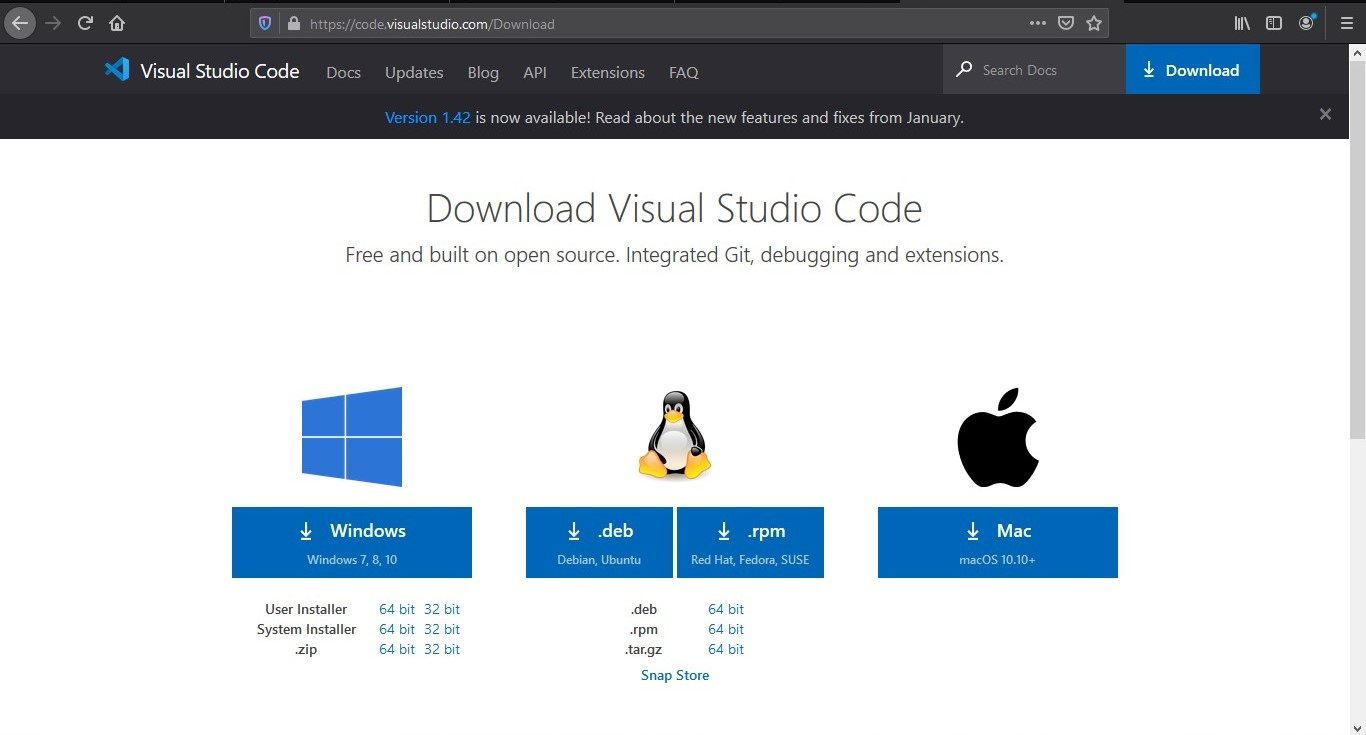
\includegraphics[scale=0.5]{Capitulo4/Documentos/imagenes_entorno/figura2-1-1.jpg}
    \caption{Ventana de descargas del editor Visual Studio Code, con el apartado .deb (paquete para equipos Linux basados en Debian) señalado.}
    \label{2.1.1}
\end{figure}

\noindent Una vez descargado el paquete se recurre a la instalación del .deb que es el requerido para la distribución que tengamos basada en Debian.  El gestor de paquetes de Ubuntu es el que controla la instalación, y para instalar Visual Studio Code se puede utilizar el centro de software de Ubuntu, el cual se muestra de manera automática cuando se hace doble clic sobre el paquete de instalación con extensión .deb. Este proceso identifica la aplicación que se desea instalar y muestra una interfaz al usuario en la que el mismo puede proceder a instalar la aplicación o a cancelar el proceso. La interfaz del centro de software de ubuntu muestra una pantalla como la de la figura \ref{2.1.2} cuando se hace doble clic sobre el paquete descargado previamente.

\begin{figure}[H]
    \centering
    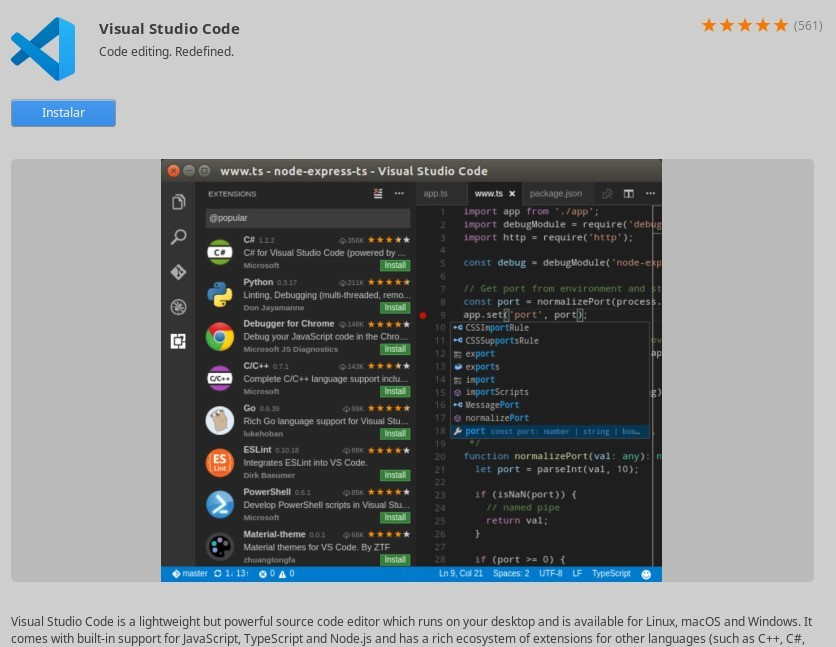
\includegraphics[scale=0.82]{Capitulo4/Documentos/imagenes_entorno/figura2-1-2.jpg}
    \caption{Instalación de Visual Studio Code mediante el centro de software de Ubuntu.}
    \label{2.1.2}
\end{figure}

\noindent Una vez concluida la instalación, para verificar que esta haya ido correctamente, se procede a abrir el editor, el cual debe mostrarse en una pantalla de inicio como la que ilustra la figura \ref{2.1.3}.

\begin{figure}[H]
    \centering
    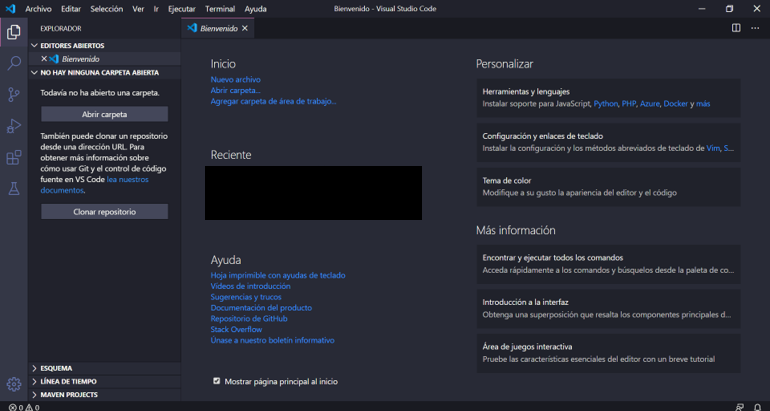
\includegraphics[scale=0.82]{Capitulo4/Documentos/imagenes_entorno/figura2-1-3.png}
    \caption{Ventana de inicio de Visual Studio Code.}
    \label{2.1.3}
\end{figure}

\subsubsection{Python en su versión 3}

\noindent El lenguaje con el que se desarrollará es Python, que para el caso de Ubuntu ya posee una versión de python instalada, para verificar esto se puede ingresar el siguiente comando en la terminal del sistema:
\begin{lstlisting}
python -V
\end{lstlisting}
La figura \ref{2.2.1} muestra el resultado de ejecutar este comando, el cual es el número de versión de python que el sistema tiene instalado en ese momento.

\begin{figure}[H]
    \centering
    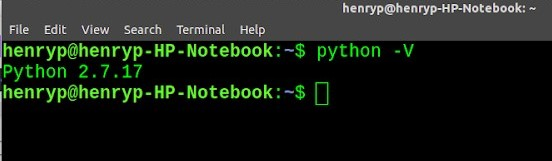
\includegraphics[scale=0.85]{Capitulo4/Documentos/imagenes_entorno/figura2-2-1.jpg}
    \caption{Resultado de la ejecución del comando para obtener la versión de python. En esta imagen se muestra que se tiene instalada la versión 2.7.}
    \label{2.2.1}
\end{figure}
\newpage
\noindent Sin embargo, para el desarrollo del sistema se requiere utilizar python en su versión 3.6.9. Para obtener esta versión en particular, se utiliza terminal para ingresar el siguiente comando:

\begin{lstlisting}
sudo add-apt-repository ppa:deadsnakes/ppa
sudo apt update
sudo apt install python3.6
\end{lstlisting}
\noindent Para corroborar la instalación de python en su versión 3.6.9, se ejecuta el comando:

\begin{lstlisting}
python3 -V
\end{lstlisting}
\noindent en la terminal del sistema. El resultado debe ser idéntico al que se puede ver señalado en la figura \ref{2.2.2}.
\begin{figure}[H]
    \centering
    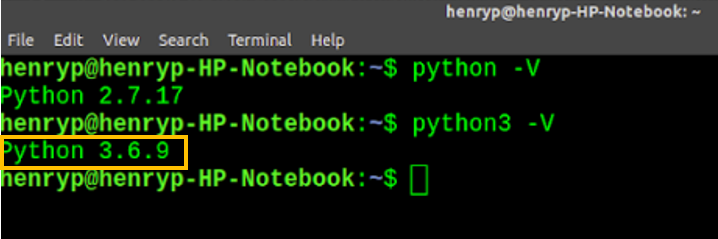
\includegraphics[scale=0.85]{Capitulo4/Documentos/imagenes_entorno/figura2-2-2.png}
    \caption{Verificación de la instalación de la versión correcta de python, se señala el resultado que indica la versión 3.6.9.}
    \label{2.2.2}
\end{figure}

\subsubsection{PIP}\\

\noindent PIP es un sistema de gestión de paquetes utilizado para instalar y administrar paquetes de software escritos en Python.\\

\noindent A partir de la instalación de python en la versión mayor a 3 (en este caso se utiliza la versión 3.6.9), PIP ya viene incluido (pero ahora es denominado PIP3), sin embargo, se puede verificar que ya se encuentra instalado ejecutando el siguiente comando en la terminal:

\begin{lstlisting}
pip3 --version
\end{lstlisting}

\noindent Como resultado de ejecutar este comando en la terminal se debe observar una respuesta del sistema similar a la que muestra la figura \ref{2.3.1}.

\begin{figure}[H]
    \centering
    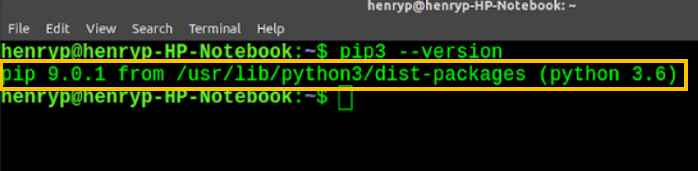
\includegraphics[scale=0.85]{Capitulo4/Documentos/imagenes_entorno/figura2-3-1.png}
    \caption{Comprobación de la instalación de PIP donde el resultado se encuentra señalado (incluso se indica para qué versión de python está configurado pip).}
    \label{2.3.1}
\end{figure}

\subsubsection{ChromeDriver}

\noindent Dado que se pretende trabajar con una biblioteca llamada Selenium, esta última requiere de un driver que sea compatible con el navegador deseado a trabajar, para el desarrollo del sistema de información, se optó por usar el navegador Google Chrome como el navegador predeterminado, para ello requerimos del driver de nombre ChromeDriver.\\

\noindent Antes de la descarga e instalación se deben de cumplir con algunos requisitos, y para instalar en ChromeDriver en el sistema operativo que se está utilizando, se debe empezar por lo ingresar los siguientes dos comandos en la terminal del sistema:
\begin{lstlisting}
sudo apt-get update
sudo apt-get install -z unzip xvfb libx16 libgconf 2-4
\end{lstlisting}

\noindent Posteriormente, se debe actualizar o instalar la versión más actual de Google Chrome, esto es más directo si se recurre a la página de descargas de Chrome, se descarga el .deb y se utiliza dicha herramienta de software para instalarlo.
La figura \ref{2.4.1} muestra la ventana de descargas del navegador. La misma página identifica el sistema operativo cuando se hace clic en el botón “Descargar Chrome”.

\begin{figure}[H]
    \centering
    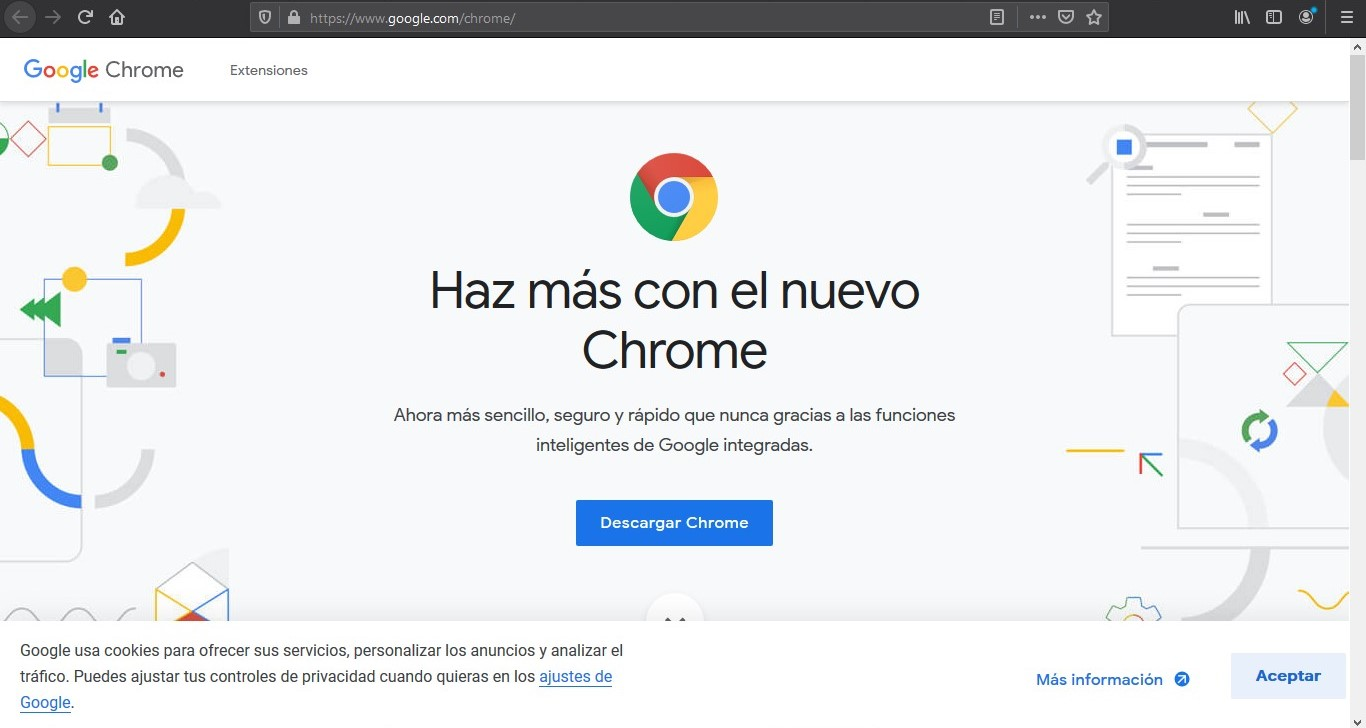
\includegraphics[scale=0.52]{Capitulo4/Documentos/imagenes_entorno/figura2-4-1.jpg}
    \caption{Página de descargas del navegador.}
    \label{2.4.1}
\end{figure}

Ya instalado el navegador, se puede continuar con el driver del navegador, para ello se visita la siguiente página:\\

\href{https://sites.google.com/a/chromium.org/chromedriver/downloads.}{https://sites.google.com/a/chromium.org/chromedriver/downloads.}\\

\noindent La figura \ref{2.4.2} ilustra una vista de la página de descargas descrita previamente.

\begin{figure}[H]
    \centering
    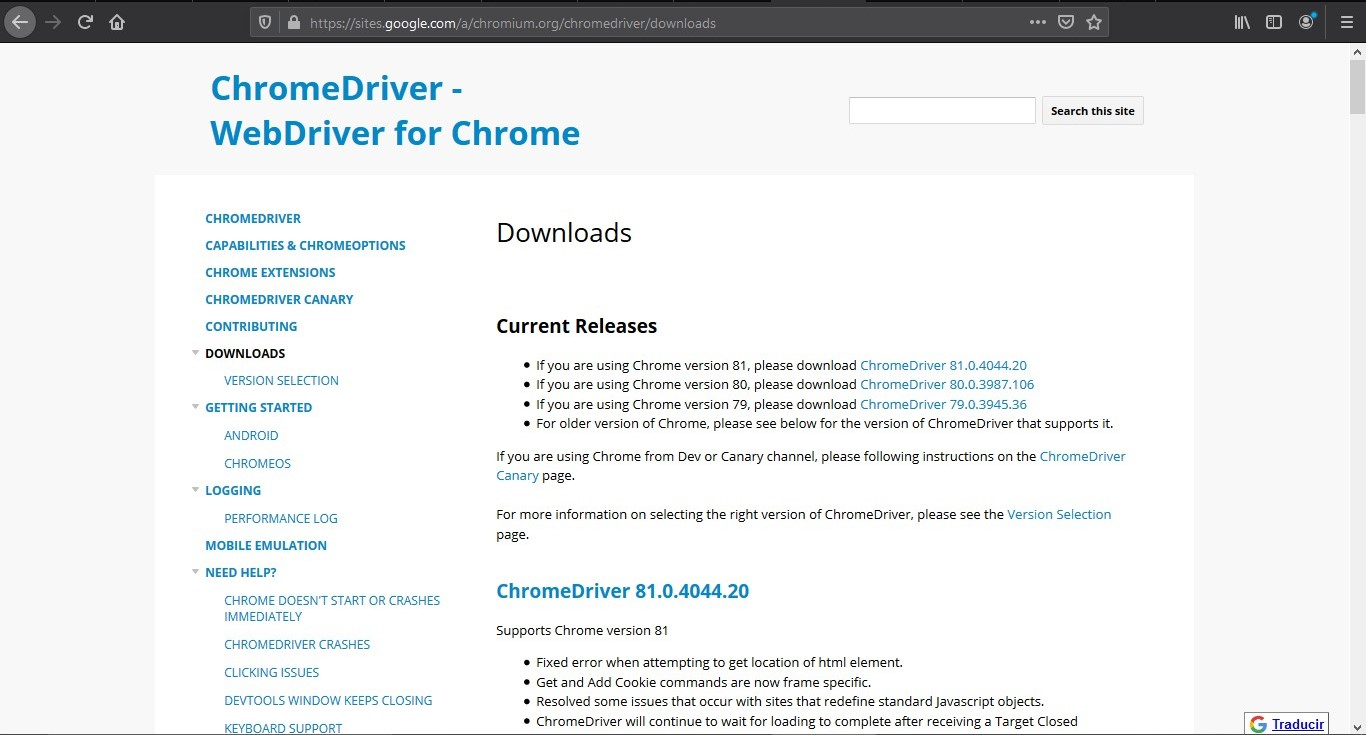
\includegraphics[scale=0.51]{Capitulo4/Documentos/imagenes_entorno/figura2-4-2.jpg}
    \caption{Página de descargas para el driver del navegador.}
    \label{2.4.2}
\end{figure}

\noindent Donde se selecciona el driver, según la versión del navegador Chrome que se tenga instalada, y se descarga el archivo. Ya con el archivo descargado, se obtiene su ubicación donde fue almacenado en el equipo y se hace clic derecho sobre el directorio seguido de la opción “Abrir en la terminal” para desplegar la pantalla de una terminal que ya esté directamente relacionada con la ruta donde se encuentra el archivo., una vez ahí, se ejecutan los siguientes comandos:

\begin{itemize}
    \item Se descomprime el .zip, cabe aclarar que se incluye en el comando, la característica del sistema, es decir los 64 bits.
\end{itemize}

\begin{lstlisting}
unzip chromedriver_linux64.zip  
\end{lstlisting}

\begin{itemize}
    \item Ya que se tiene el contenido, se realiza la instalación en el PATH:
\end{itemize}
\begin{lstlisting}
sudo mv chromedriver /usr/bin/chromedriver
sudo chown root:root /usr/bin/chromedirver
sudo chmod +x /usr/bin/chromedriver
\end{lstlisting}
\noindent Finalizado todo ya se cuenta con el driver necesario para la adquisición de los datos a través del navegador.
}
\\

\subsubsection{MGLTools}

\noindent MGLTools es un software desarrollado en el Laboratorio de Gráficos Moleculares (MGL) del Instituto de Investigación Scripps para la visualización y análisis de estructuras moleculares.
Utilizaremos esta herramienta para la transformación de las estructuras moleculares de los compuestos y las proteínas, esto  con la finalidad de generar receptores que puedan acoplarse a una estructura de un ligando.\\

\noindent Ejecutando la siguiente lista de comandos podremos descargar esta herramienta:
\begin{lstlisting}
wget http://mgltools.scripps.edu/downloads/downloads/tars
/releases/REL1.5.6/mgltools_x86_64Linux2_1.5.6.tar.gz
tar -xzvf mgltools_x86_64Linux2_1.5.6.tar.gz
cd mgltools_x86_64Linux2_1.5.6
./install.sh
cd MGLToolsPckgs/AutoDockTools/Utilities24
sudo cp prepare_ligand4.py /usr/local/bin
sudo cp prepare_receptor4.py /usr/local/bin
sudo cp prepare_gpf4.py /usr/local/bin
cd ../../..
cd bin
sudo cp pythonsh /usr/local/bin
\end{lstlisting}


\subsubsection{AutoDock-Vina}\\

\noindent AutoDock Vina es un conjunto de herramientas de acoplamiento automatizadas. Está diseñado para predecir cómo las moléculas pequeñas, como sustratos o candidatos a fármacos, se unen a un receptor de estructura 3D conocida.\\

\noindent Esta herramienta sera utilizada para realizar un docking más preciso introduciendo las estructuras del ligando y el receptor.
Para realizar su instalación ejecutaremos la siguiente lista de comandos:
\begin{lstlisting}
sudo wget http://vina.scripps.edu/download/autodock_vina_1_1_2_linux_x86.tgz
echo descomprimir
tar -xzvf autodock_vina_1_1_2_linux_x86.tgz
cd autodock_vina_1_1_2_linux_x86/bin
cp vina /usr/local/bin
\end{lstlisting}

\subsubsection{AutoGrid}\\

\noindent AutoGrid es un programa que calcula previamente los mapas de cuadrícula de las energías de interacción para varios tipos de átomos, como los carbonos alifáticos, los carbonos aromáticos, los oxígenos de enlace de hidrógeno, etc., con una macromolécula como una proteína, ADN o ARN.\\

\noindent Estos mapas de cuadrícula se utilizan luego en los cálculos de acoplamiento de AutoDock para determinar la energía de interacción total para un ligando con una macromolécula.

\noindent Para la instalación de esta herramienta, ejecutamos la siguiente lista de comandos en la terminal:
\begin{lstlisting}
sudo wget http://autodock.scripps.edu/downloads/
autodock-registration/tars/dist426/
autodocksuite-4.2.6-x86_64Linux3.tar
echo Descomprimiendo autodocksuite
tar -xvf autodocksuite-4.2.6-x86_64Linux3.tar
cd x86_64Linux3
cp autodock4 /usr/local/bin
cp autogrid4 /usr/local/bin
\end{lstlisting}
\subsection{Bibliotecas}{
\noindent La instalación de bibliotecas se realiza utilizando el administrador de paquetes para python PIP en su versión para python3 el cual corresponde al comando de pip3, cuya instalación se menciona en el apartado X. Es importante señalar que para todas las bibliotecas que se van a instalar se requiere conexión a internet. Para verificar la correcta instalación de cada biblioteca, basta con dar seguimiento a la información que el sistema va mostrando mientras se encuentra instalando la biblioteca especificada. Las bibliotecas aquí descritas cuando han sido correctamente instaladas muestran un mensaje (definido por pip3) como el que se señala en la figura \ref{3.1}, donde se toma como ejemplo la instalación de la biblioteca Requests, y al final puede leerse la frase en inglés “Successfully installed” seguido del nombre completo de la biblioteca.

\begin{figure}[H]
    \centering
    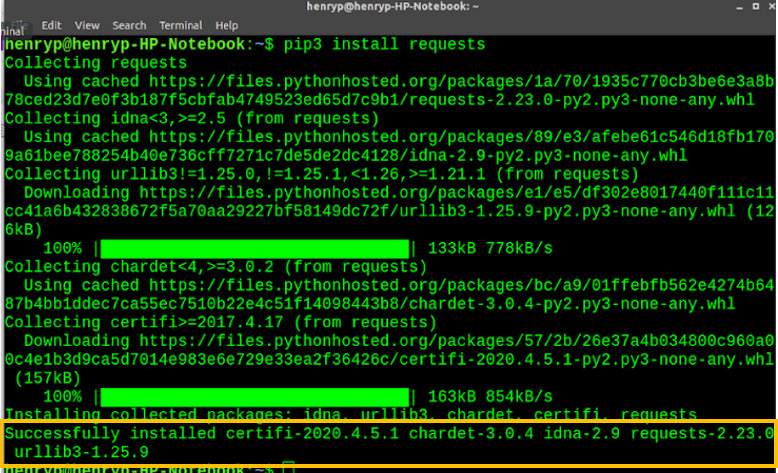
\includegraphics[scale=0.85]{Capitulo4/Documentos/imagenes_entorno/figura3-1.png}
    \caption{Instalación exitosa de la biblioteca Requests, donde se señala el mensaje que arroja pip3 de éxito del proceso de instalación.}
    \label{3.1}
\end{figure}
\subsubsection{Tkinter}\\

\noindent Con Python hay muchas posibilidades para programar una interfaz gráfica de usuario (GUI) pero Tkinter es fácil de usar, es multiplataforma y, además, viene incluido con Python en su versión para Windows, para Mac y para la mayoría de las distribuciones GNU/Linux. Se le considera el estándar de facto en la programación GUI con Python.\\

\noindent Tkinter es un binding de la biblioteca Tcl/Tk que está también disponible para otros lenguajes como Perl y Ruby.
A pesar de su larga historia, su uso no está demasiado extendido entre los usuarios de equipos personales porque su integración visual con los sistemas operativos no era buena y proporcionaba pocos widgets (controles) para construir los programas gráficos.
Para instalar Tkinter se debe escribir y ejecutar el siguiente comando en la terminal:
\begin{lstlisting}
sudo apt-get install python3-tk
\end{lstlisting}
\noindent Para verificar esta instalación, se procede a ingresar a la línea de comandos de python3 simplemente ejecutando en la terminal el comando:
\begin{lstlisting}
python3 
\end{lstlisting}
\noindent Luego se procede a escribir las siguientes dos líneas:
\begin{lstlisting}
import tkinter
tkinter.TkVersion
\end{lstlisting}
\noindent Si la instalación se ha hecho correctamente, la terminal arroja un resultado como el que se señala en la figura \ref{3.1.1}.

\begin{figure}[H]
    \centering
    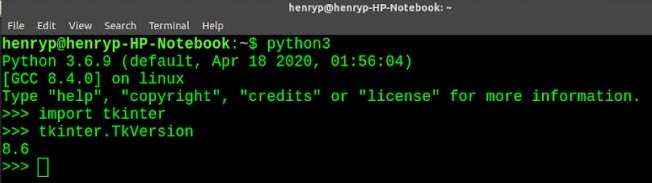
\includegraphics[scale=0.85]{Capitulo4/Documentos/imagenes_entorno/figura3-1-1.jpg}
    \caption{Confirmación de la instalación de Tkinter.}
    \label{3.1.1}
\end{figure}
\subsubsection{Requests}\\

\noindent Requests es una librería de Python para peticiones HTTP liberada bajo una la licencia de Apache License 2.0.  Request permite enviar solicitudes HTTP / 1.1 con extrema facilidad.\\ 

\noindent No es necesario agregar manualmente cadenas de consulta a sus URL, ni codificar de forma estricta los datos POST. Keep-alive y el grupo de conexiones HTTP son 100\% automáticas.\\

\noindent La instalación en Linux es de la siguiente manera. Como ya se ha instalado PIP en la versión para python3, basta con el siguiente comando:\\

\begin{lstlisting}
pip3 install requests
\end{lstlisting}

\subsubsection{Selenium}\\

\noindent Selenium para Python proporcionan una API simple para navegar o realizar pruebas en algún navegador web, utilizando un WebDriver. A través de Selenium Python API puede acceder a todas las funcionalidades de Selenium WebDriver de una manera sencilla e intuitiva.\\
Selenium Python proporcionan una API conveniente para acceder a Selenium WebDrivers como Firefox, Internet Explorer, Chrome, Remote, etc. Y es compatible con versiones de Python desde la 2.7.\\

\noindent
Para la instalación se ejecuta el siguiente comando en la terminal del sistema:
\begin{lstlisting}
pip3 install selenium
\end{lstlisting}

\subsubsection{Pillow}\\

\noindent Es una librería gratuita que permite la edición de imágenes directamente desde Python. Soporta una variedad de formatos, incluidos los más utilizados como GIF, JPEG y PNG. Una gran parte del código está escrito en C, por cuestiones de rendimiento.\\

\noindent Debido a que la librería soporta únicamente hasta la versión 2.7 de Python y, al parecer, no se propuso avanzar con él, un equipo de desarrolladores en colaboración se ha desarrollado Pillow, una bifurcación, con un desarrollo más «amigable», así nace PIL que pretende mantener una librería estable y que se adapte a las nuevas tecnologías (De Python 3 en adelante). Por esta razón, PIL entró en función en lugar de Pillow.\\

\noindent Para proceder con la instalación, se ingresa y ejecuta el siguiente comando en la terminal del sistema:

\begin{lstlisting}
pip3 install Pillow
\end{lstlisting}

\subsubsection{BioPython}

\noindent BioPython es el nombre que recibe una serie de aplicaciones y programas informáticos pensados para cuantificar y hacer cálculos con datos biológicos, programados por una comunidad internacional. El uso de esta biblioteca apoya en aportar el mayor número posible de bibliotecas informáticas basadas en el lenguaje de programación Python, que usualmente para tener aplicaciones bioinformáticas y que estén disponibles para un público lo más amplio posible.\\

\noindent Se hace uso de BioPython ya que   permite representar secuencias biológicas y anotaciones de genomas y es capaz de comunicar con las bases de datos biológicos en línea del NCBI para hacer cálculos. Además, gracias a diversos módulos, puede ser utilizada para trabajar sobre proyectos relativos al alineamiento de secuencias, cálculo de estructuras proteicas, genética de poblaciones, filogenética e inteligencia artificial.\\

\noindent Para instalarlo, se puede realizar a través de los comandos, cabe mencionar que las versiones recientes de Python (comenzando con Python 2.7.9 y Python 3.4) incluyen la herramienta de administración de paquetes Python, que permite una instalación fácil desde la línea de comandos en todas las plataformas:
\begin{lstlisting}
pip3 install biopython
\end{lstlisting}

\subsubsection{PubChemPy}\\

\noindent La biblioteca PubChemPy proporciona una forma de interactuar con la base de datos PubChem en Python. Permite búsquedas químicas por nombre, subestructura y similitud, estandarización química, conversión entre formatos de archivos químicos, representación y recuperación de propiedades químicas.\\
 
\noindent Para la instalación se procede a ejecutar el siguiente comando en la terminal del sistema:
\begin{lstlisting}
pip3 install pubchempy
\end{lstlisting}
\noindent Esencialmente esta biblioteca consta de realizar solicitudes a servidores de esta plataforma, dicha solicitud se evalúa y luego se envía una respuesta. Sin embargo pueden haber algunos inconvenientes, se requiere una conexión constante a Internet y algunas tareas serán más lentas que si se realizan localmente en una propia computadora. Por lo que estos requerimientos, se deben de contemplar al codificar.

\subsubsection{Pypdb}

\noindent Una interfaz de programación Python para el Banco de datos de proteínas RCSB (PDB) que permite la búsqueda y recuperación de datos para una amplia gama de tipos de resultados, incluidas BLAST y consultas de secuencias.\\

\noindent La API se auxilia de XML existente y funciona creando solicitudes personalizadas a partir de tipos nativos de Python, lo que permite la extensibilidad y la modificación directa. La librería tiene la capacidad de realizar muchos tipos de búsqueda avanzada del Banco de datos de proteínas que, de lo contrario, solo están disponibles a través del sitio web de PDB.\\

Basta con ejecutar el siguiente comando en la terminal del sistema:
\begin{lstlisting}
pip3 install pypdb
\end{lstlisting}

\subsubsection{Ratelimit}

\noindent Las API son una forma muy común de interactuar con los servicios web. A medida que crece la necesidad de consumir datos, también lo hace la cantidad de llamadas API necesarias para mantenerse actualizado con las fuentes de datos. Sin embargo, muchos proveedores de API impiden que los desarrolladores realicen demasiadas llamadas a la API. Esto se conoce como limitación de velocidad y, en el peor de los casos, se puede prohibir que su aplicación realice más llamadas API si abusa de estos límites.\\

\noindent Este paquete presenta un decorador de funciones que evita que una función se llame con más frecuencia que la permitida por el proveedor de API. Esto debería evitar que los proveedores de API prohíban sus aplicaciones conforme a sus límites de velocidad.\\

\noindent Utilizando el siguiente comando en la terminal se instala la biblioteca ratelimit:

\begin{lstlisting}
pip3 install ratelimit
\end{lstlisting}
}
\\
\subsubsection{Pandas}

\noindent Pandas es un paquete de Python de código abierto que proporciona numerosas herramientas para el análisis de datos. El paquete viene con varias estructuras de datos que se pueden usar para muchas tareas diferentes de manipulación de datos. También tiene una variedad de métodos que se pueden invocar para el análisis de datos, lo cual es útil cuando se trabaja en ciencia de datos y problemas de aprendizaje automático en Python.\\

Para realizar la instalación de esta biblioteca, se ejecuta el siguiente comando en la terminal:\\

\begin{lstlisting}
pip3 install pandas
\end{lstlisting}

\subsubsection{Scikit-learn}

\noindent Scikit-learn proporciona una gama de algoritmos de aprendizaje supervisados ​​y no supervisados ​​a través de una interfaz consistente en Python.
Se licencia bajo una licencia BSD simplificada permisiva y se distribuye bajo muchas distribuciones de Linux, fomentando el uso académico y comercial.
La biblioteca está construida sobre SciPy (Scientific Python) que debe instalarse antes de poder usar scikit-learn. Esta pila que incluye:

\begin{itemize}
    \item NumPy: paquete de matriz base n-dimensional
    \item SciPy: biblioteca fundamental para la computación científica
    \item Matplotlib: trazado 2D / 3D completo
    \item IPython: consola interactiva mejorada
    \item Sympy: matemática simbólica
    \item Pandas: estructuras de datos y análisis
\end{itemize}

\noindent Las extensiones o módulos para SciPy se denominan convencionalmente SciKits. Como tal, el módulo proporciona algoritmos de aprendizaje y se llama scikit-learn.
La visión de la biblioteca es un nivel de robustez y soporte requerido para su uso en sistemas de producción. Esto significa un enfoque profundo en preocupaciones tales como la facilidad de uso, la calidad del código, la colaboración, la documentación y el rendimiento.\\

\noindent Para instalar el paquete de bibliotecas de scikit-learn se ejecuta en la terminal del equipo el siguiente comando:

\begin{lstlisting}
pip3 install scikit-learn
\end{lstlisting}

\subsubsection{NumPy}{
\noindent NumPy es el paquete fundamental para la computación científica en Python. Es una biblioteca de Python que proporciona un objeto de matriz multidimensional, varios objetos derivados (como matrices y matrices enmascaradas), y una variedad de rutinas para operaciones rápidas en matrices, que incluyen matemática, lógica, manipulación de formas, clasificación, selección, E / S , transformadas discretas de Fourier, álgebra lineal básica, operaciones estadísticas básicas, simulación aleatoria y mucho más.\\

Para instalar esta biblioteca se ejecuta en la terminal del equipo el siguiente comando:

\begin{lstlisting}
pip3 install numpy
\end{lstlisting}
}
}
%% ------------------- Generación del Código de los Componentes y Procedimientos --------------------------------------- %%
\section{Generación del Código de los Componentes y Procedimientos}
 \noindent Este documento describe el diseño de la lógica de programación y los algoritmos utilizados para la solución de los diversos problemas que implicaba la generación del código de los componentes de SisPAF.\\
 
 \noindent SisPAF es un sistema compuesto por 3 módulos principales, cada uno contando con su propio desarrollo para la interfaz y para el código que acompaña dicha interfaz. La figura X ilustra el modelo lógico del sistema donde se pueden observar los 3 módulos antes mencionados, los cuales son:\\
 
 \subsubsection{Búsqueda de información:}\label{Busqueda}
 \noindent El módulo de búsqueda de información es el primer módulo de SisPAF y es el encargado de obtener la información necesaria para realizar la predicción de la actividad farmacológica (efectividad de los fármacos frente a cierta patología).\\
 
 \subsubsection{Análisis de la información:}
\noindent Una vez obtenidos los datos del módulo de búsqueda y que el usuario es informado de los resultados de dicha búsqueda, se procede a realizar un análisis de la información obtenida. Para esto se empleo el uso de un método de la bioinformática conocido como modelo QSAR (por sus siglas en inglés, \textit{Quantitative Structure Activity Relationship}) que permite relacionar a los compuestos con determinadas proteínas y predecir qué tan efectivos pueden ser para atacar y destruir esas proteínas. Dentro del mismo modelo QSAR se utilizan algoritmos de \textit{Machine Learning}, en este caso regresión lineal múltiple y mapa auto-organizado para generar los resultados que representan la efectividad de los compuestos, previamente mencionada.

\subsubsection{Generación de resultados:}
\noindent En este módulo, los resultados del análisis son ordenados y desplegados al usuario en una interfaz, para su visualización con opción a ser almacenados en el sistema.

\begin{figure}[H]
    \centering
    \includegraphics[scale=0.40]{Capitulo4/Documentos/imagenes_generacion/modeloDatosLogico.png}
    \caption{Modelo lógico de SisPAF.}
    \label{Modelo_logico_de_SisPAF_1}
\end{figure}

\subsubsection{Generación de código de los componentes}
\subsection{Búsqueda de información}
\noindent Este módulo incluye desde la ventana de inicio de SisPAF (descrita en el apartado \ref{Busqueda}) hasta la confirmación de los resultados de la búsqueda. El usuario ingresa un archivo inicial (véase en la tabla \ref{diccionario}) o indica un directorio donde se encuentre un proyecto ya existente.  SisPAF analiza ya sea el directorio o el archivo inicial y recopila información sobre los compuestos y proteínas de los que se desean obtener datos en específico (estructura molecular de los compuestos, estructura molecular de las proteínas, descriptores físico químicos de los compuestos, mecanismos de acción de los compuestos). Cuando SisPAF determina los elementos (compuestos y proteínas indicados por el usuario) de los cuales debe obtener dichos datos, realiza las conexiones correspondientes con las bases de datos en línea que proveen esa información (en la figura \ref{DFD1} se observan las 3 bases de datos, DrugBank, PDB,  PubChem, y la información que de ellas se obtiene). Finalmente se despliega al usuario una tabla con un resumen de qué datos se obtuvieron para cada uno de los elementos identificados.\\

\noindent El diagrama de flujo que ilustra la figura \ref{DFD1}. muestra las actividades que componen al módulo de búsqueda de información, las cuales de describen a continuación.

\begin{figure}[H]
    \centering
    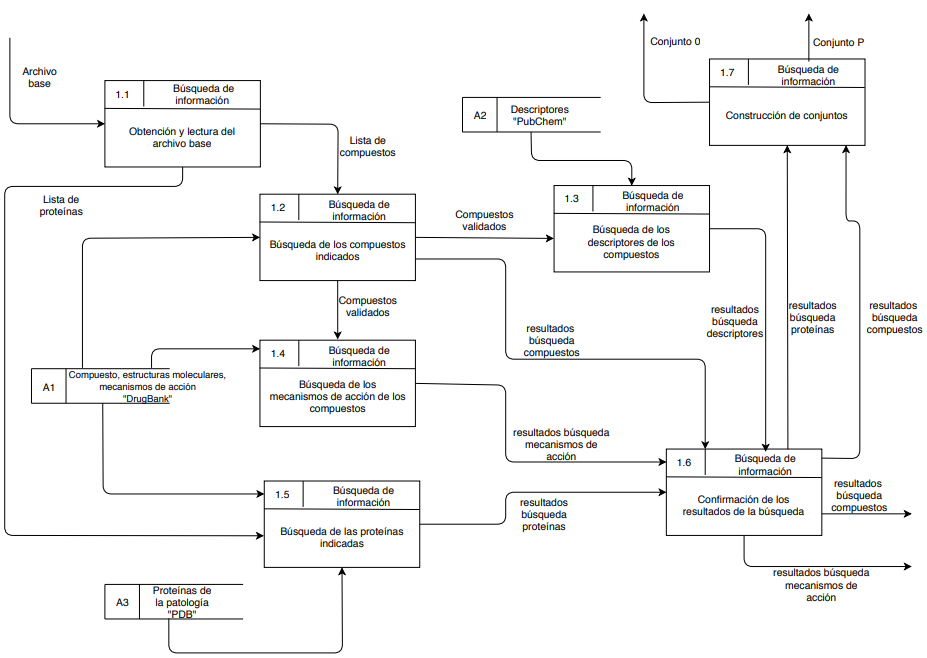
\includegraphics[scale=0.46]{Capitulo2/images/DFD-1.png}
    \caption{Diagrama de flujo de datos del módulo de búsqueda de información.}
    \label{DFD1}
\end{figure}
%%%%%%%%%%%%%%%%%%%%%%%%%%%%%%%%%%%%%%%%%%%%%%%%%%%%%%%%%%%%%%%
\subsubsection{Diseño de interfaces}{
\noindent Al momento de  realizar el análisis y diseño del sistema de información,  se plantearon las vistas que tendrían las interfaces, empezando por las que comunican al usuario con las funciones más importantes del sistema, como la adquisición del archivo inicial, si existe un  error en este, entre otras interacciones importantes al iniciar SisPAF.\\

\noindent A continuación mostramos las pantallas que se consideran importantes, y el resultado al ser programadas en el lenguaje Python, auxiliándose en la librería Tkinter.

\begin{figure}[H]
    \centering
    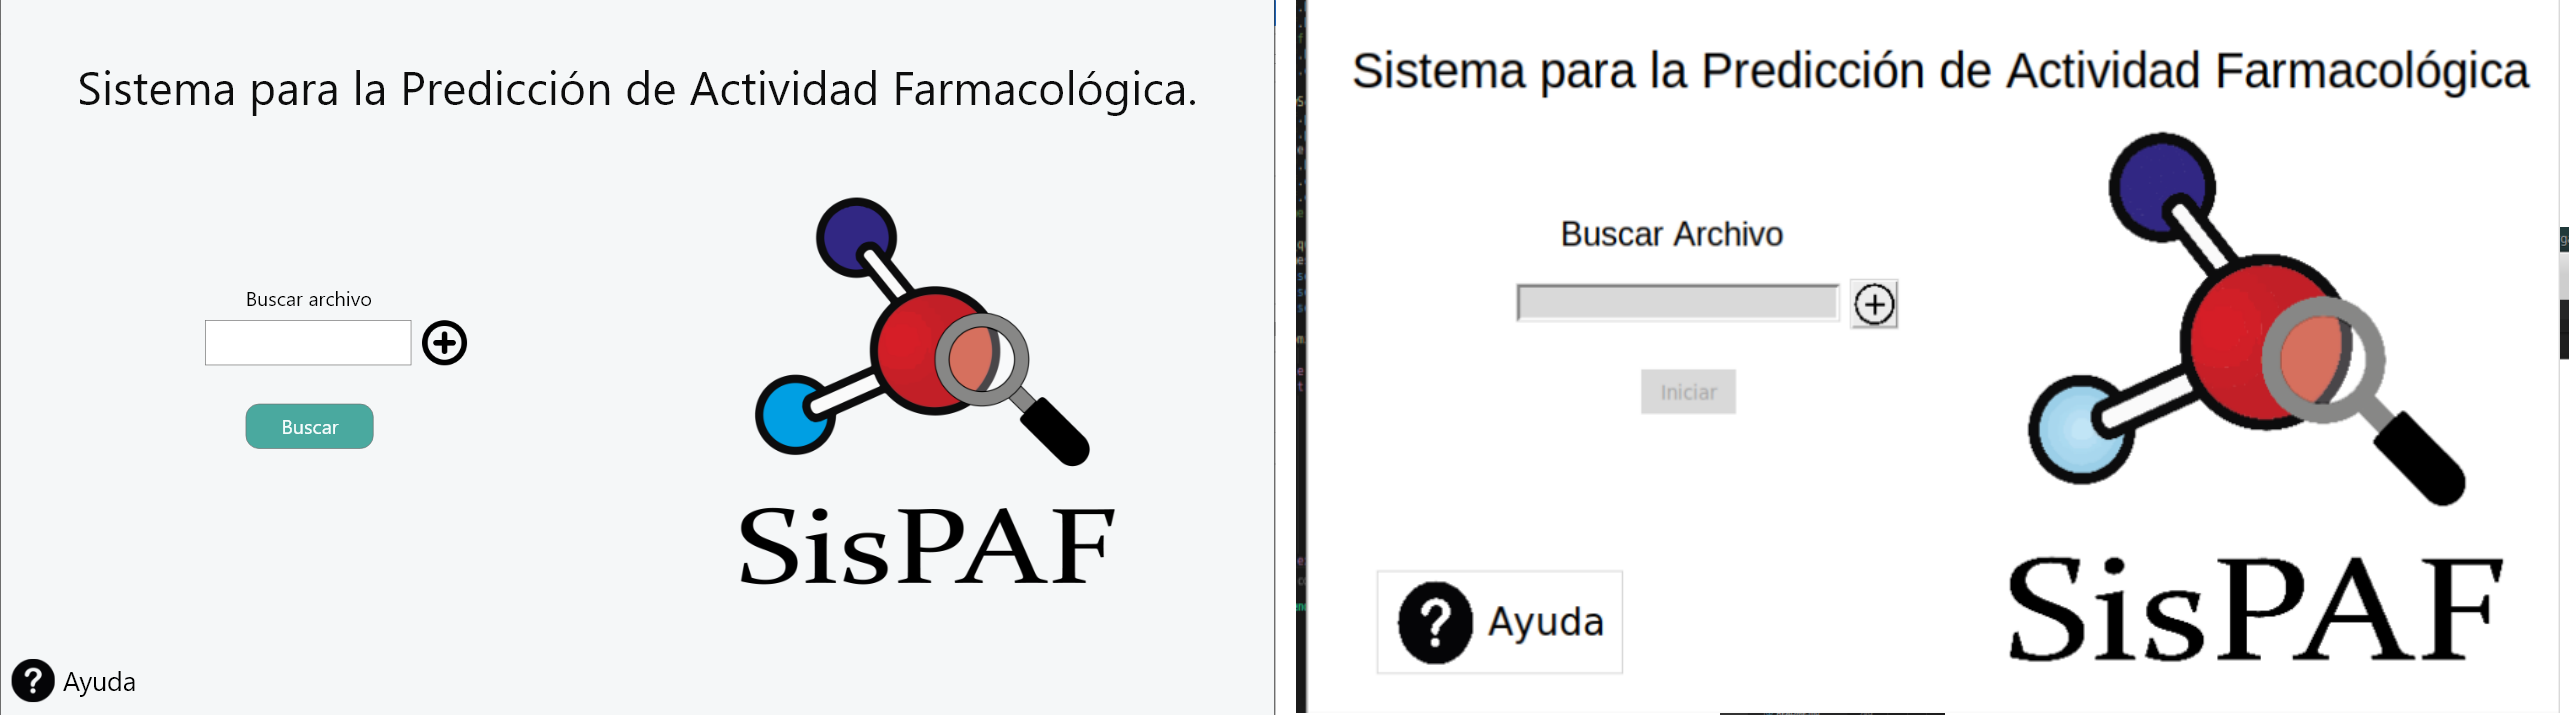
\includegraphics[scale=0.215]{Capitulo4/Documentos/imagenes_generacion/ComparacionPan1.png}
    \caption{Comparación de pantallas, a la izquierda la diseñada y  a la derecha la pantalla programada.}
    \label{comparacion}
\end{figure}

\noindent A esas pantallas se han incluido mensajes de error, que igual estaban planificados para cuando existieran posibles fallos, uno de ellos, es cuando el archivo no contiene el formato y/o contenido adecuado.\\

\begin{figure}[H]
    \centering
    
\includegraphics[scale=0.375]{Capitulo4/Documentos/imagenes_generacion/PickwrongAr.png}
    \caption{Comparación de mensajes de error, a la izquierda la planeada y a la derecha la programada.}
    \label{comparacion_2}
\end{figure}

}
%%%%%%%%%%%%%%%%%%%%%%%%%%%%%%%%%%%%%%%%%%%%%%%%%%%%%%%%%%%%%%
\subsubsection{Inicio}{
\noindent La interfaz de inicio funciona como una especie de canalizador. Dependiendo de si el usuario quiere crear un nuevo proyecto o abrir uno ya existente, los procesos a ejecutar son diferentes hasta que se llega a la parte del análisis de información. Para comenzar, cualquier botón solicita al usuario que seleccione un directorio (para crear o para abrir un proyecto). Si se desea crear un nuevo proyecto se procede a mostrar la interfaz correspondiente que le permite al usuario cargar al sistema un archivo inicial y comenzar con el proceso de la búsqueda de información. Por otro lado si el usuario elige abrir un proyecto el sistema solicita que se le indique el directorio donde se encuentra dicho proyecto y procede a analizar la estructura del directorio para definir la información que ya se ha obtenido y continuar el proceso desde el punto necesario.\\
}
%%%%%%%%%%%%%%%%%%%%%%%%%%%%%%%%%%%%%%%%%%%
\subsubsection{Obtención y lectura del archivo inicial}{
\noindent El proceso para realizar la obtención y la lectura del archivo inicial (véase \ref{diccionario}) involucra la comunicación de la interfaz que es la que determina dónde se va a almacenar dicho archivo y el uso de herramientas básicas de lectura y escritura presentes en python. Python permite abrir un archivo simplemente con especificar la ruta donde se encuentra almacenado. Luego se realiza la lectura del archivo mediante un ciclo que lee línea por línea hasta que se encuentra con el final de dicho archivo. Durante esta lectura es donde es posible almacenar la información requerida en dos secciones separadas, en este caso una sección para compuestos y una para proteínas. Estos dos apartados definen los elementos cuya información debe ser buscada en la base de datos en línea.
En este proceso se hace presente la comprobación de la estructura del archivo inicial, la cual es representada de manera gráfica por la figura \ref{flujo}.\\


\noindent La figura \ref{flujo} contiene el diagrama de flujo para el proceso de comprobación del archivo inicial, el cual se basa en revisar la presencia de las etiquetas (Compounds y Proteins) y enviar una alerta al usuario en caso de que no se encuentren dichas etiquetas. El mismo SisPAF, al momento de leer y almacenar la información del archivo inicial, es capaz de detectar elementos duplicados, haciendo que los elementos obtenidos sean únicos.

\begin{figure}[H]
    \centering
    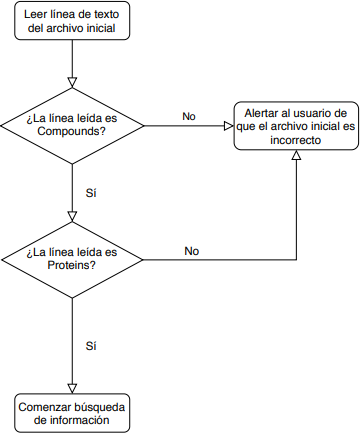
\includegraphics[scale=0.85]{Capitulo4/imagenes/diagramaArchivoInicia.png}
    \caption{Diagrama de flujo del análisis del archivo inicial.}
    \label{flujo}
\end{figure}
}
%%%%%%%%%%%%%%%%%%%%%%%%%%%%%%%%%%%%%%%%%%%%%%%%%%%%%
\subsubsection{Diseño de interfaces}{
\noindent Para el módulo de la búsqueda de datos, se diseñaron interfaces que muestran el status del sistema durante la conexión a las bases de datos, mostrar el resultado de dichas consultas, dándole a saber al usuario si hubo un error en la adquisición de la información necesario de los compuestos o las proteínas.\\

\noindent A continuación se muestra la pantalla de espera, mientras el sistema realiza la búsqueda de información, con la cual se le indica al usuario que el sistema sigue trabajando.
}

\begin{figure}[H]
    \centering
    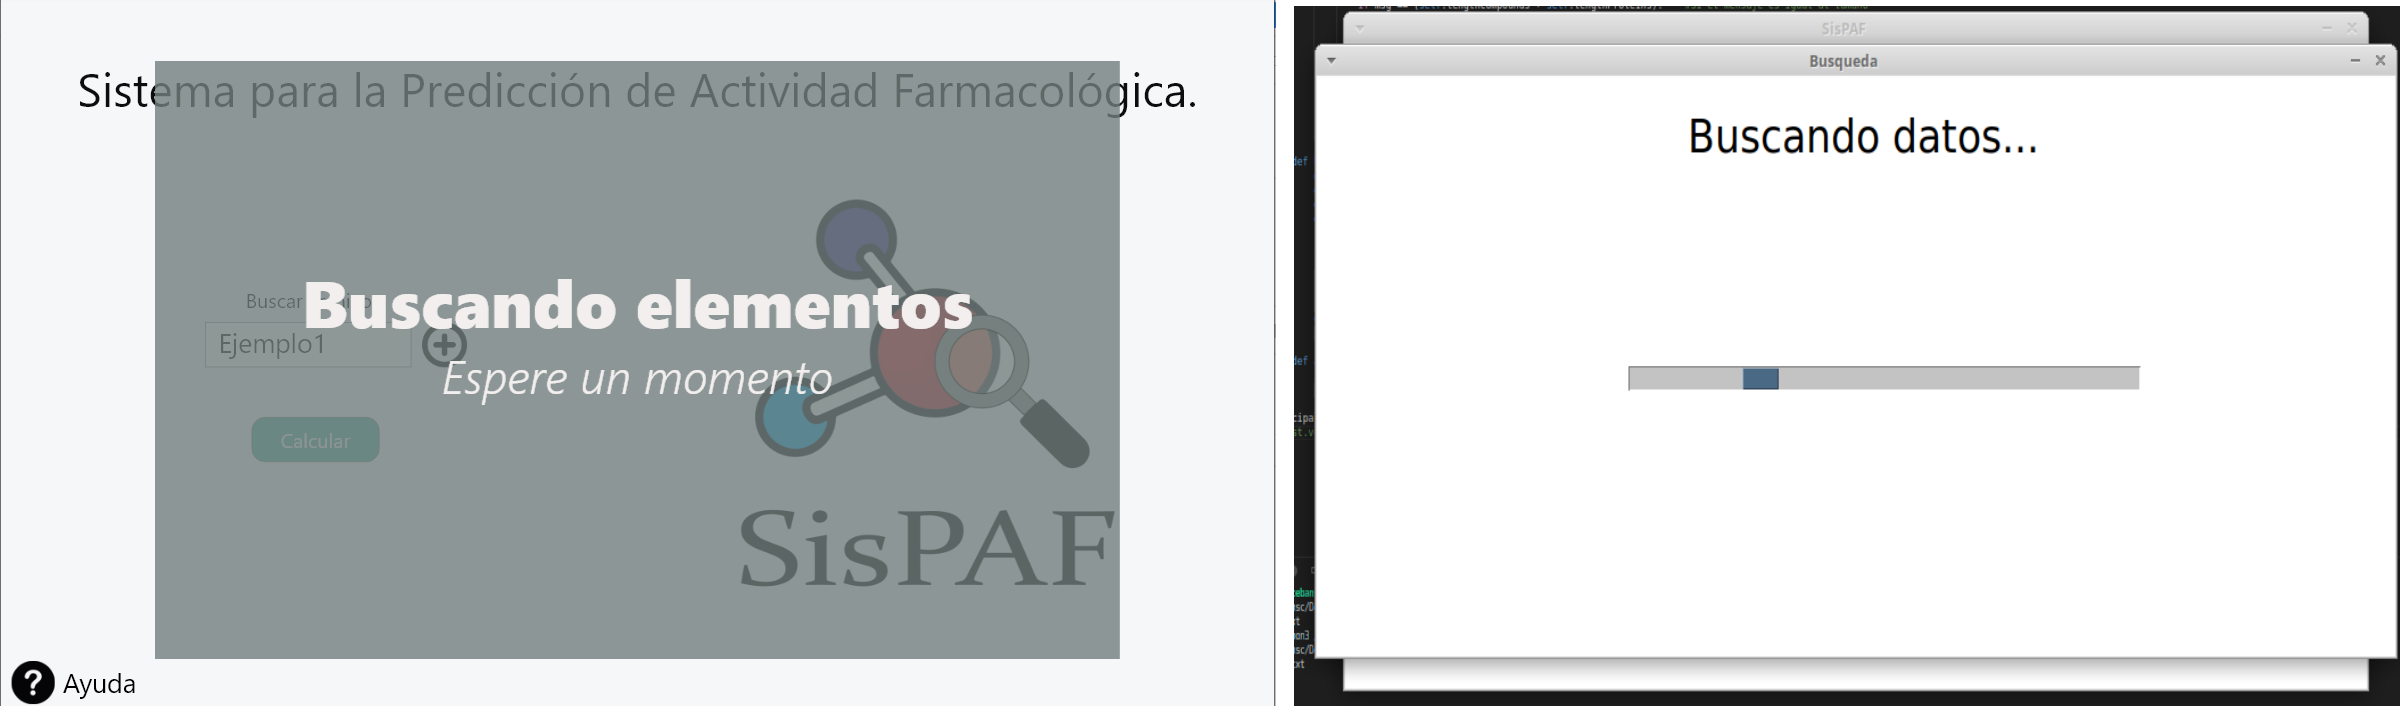
\includegraphics[scale=0.235]{Capitulo4/Documentos/imagenes_generacion/Esperabusqueda.png}
    \caption{Comparación de pantallas de espera para la búsqueda de información, a la izquierda la planeada y a la derecha la programada.}
    \label{comparacion_3}
\end{figure}

\noindent Durante la búsqueda, el mayor problema, incluso considerarse fatal, sería la pérdida de conexión a internet, para ello se planeó en un inicio la aparición de un mensaje de error para cuando esto suceda.

\begin{figure}[H]
    \centering
    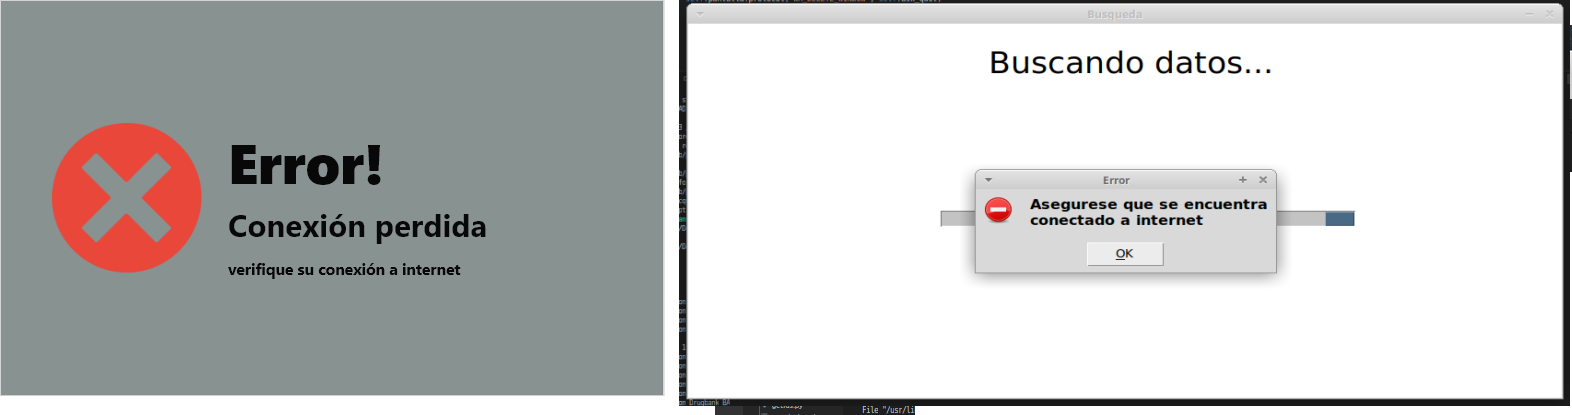
\includegraphics[scale=0.375]{Capitulo4/Documentos/imagenes_generacion/errorNet.png}
    \caption{Comparación de mensajes de error en la pérdida de conexión, a la izquierda la planeada y a la derecha la programada.}
    \label{comparacion_4}
\end{figure}

\noindent Cuando la búsqueda de datos, ha finalizado, al usuarios se muestra una pantalla que indica el estado de cada compuesto y proteína respecto a la información que nos interesa de ellos, si no se encontró la estructura del compuesto, o de la proteína, etc.

\begin{figure}[H]
    \centering
    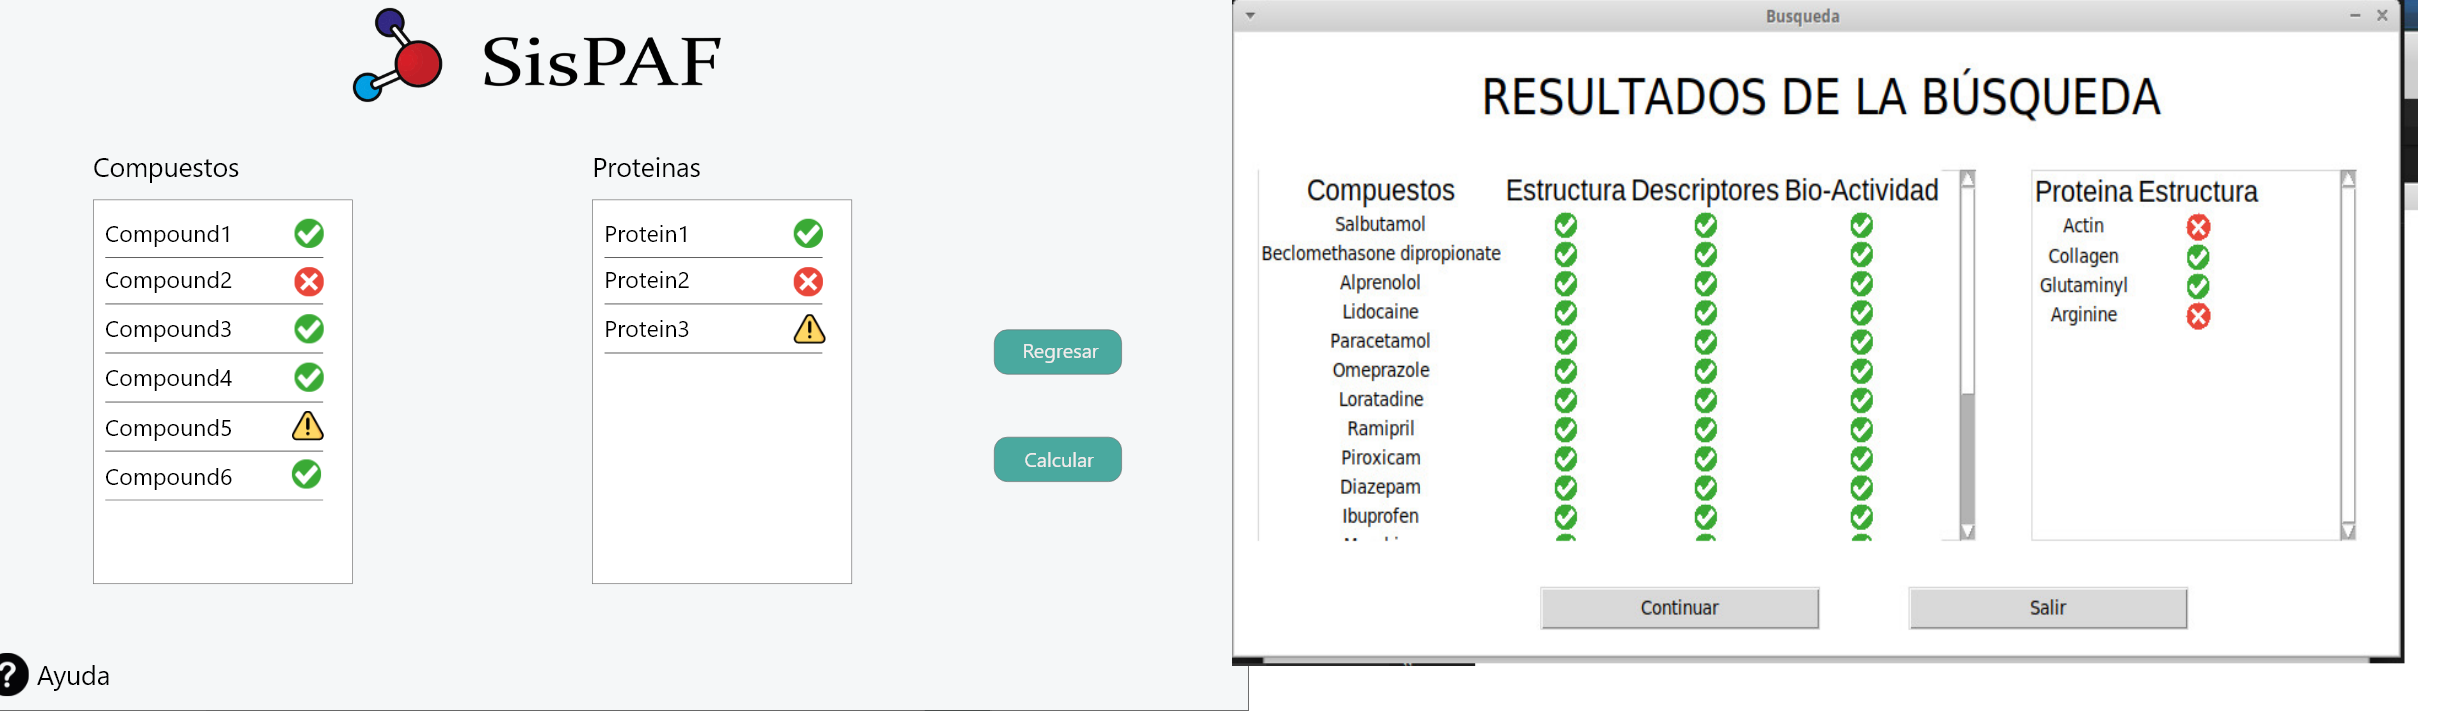
\includegraphics[scale=0.225]{Capitulo4/Documentos/imagenes_generacion/ResultBusqueda.png}
    \caption{Comparación de pantallas para resultados de búsqueda, a la izquierda la planeada y a la derecha la programada.}
    \label{comparacion_5}
\end{figure}
%%%%%%%%%%%%%%%%%%%%%%%%%%%%%%%%%%%%%%%%%%%%%%%%%%%%%%%%%%%%%%
\subsubsection{Búsqueda de información: uso de API’s y Web scrapping}
\noindent Cuando ya se han definido los elementos de los cuales se debe obtener su información, se procede a utilizar API’s que las bases de datos en línea poseen y que utilizan para consultar la información de dichas bases de datos. Para realizar las llamadas a las API se deben tomar en cuenta dos cosas: la cantidad límite de peticiones por segundo que cada API define para evitar saturarse de solicitudes y la manera en cómo debe accederse a la información que se requiere obtener (para este caso, la estructura molecular, los descriptores fisicoquímicos computados y los mecanismos de acción para cada uno de los  compuestos, mientras que para las proteínas solo se requiere la estructura molecular).

\noindent En esta situación python provee de bibliotecas que permiten realizar las peticiones a las API de una forma más sencilla y eficaz que de la manera tradicional, pues dichas bibliotecas están enfocadas solo a trabajar con las API’s de las bases de datos en cuestión (PDB, PubChem).

\noindent Para el caso de las proteínas, el dato de mayor importancia, es su estructura, la cual se requiere en formato pdb, que brinda la suficiente información de la proteína para realizar todos cálculos necesarios,  al requerirse un formato pdb, nos valemos de la base de datos de Protein Data Bank, el proceso de obtención, consiste en adquirir el nombre de la proteína, comparar de entre todas las proteínas existentes en la base de datos el nombre exacto de la proteína que empate mejor con la proporcionada por el usuario, cuando ya se obtiene un nombre, se consigue el ID de PDB para poder obtener todo el archivo que contiene la estructura, es un poco mejor visualizado en el diagrama.\\


\begin{figure}[H]
    \centering
    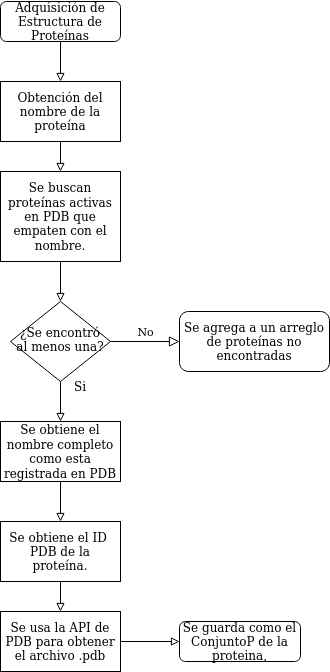
\includegraphics[scale=0.75]{Capitulo4/Documentos/imagenes_generacion/EstructuraPro.png}
    \caption{Diagrama de flujo de adquisición de la estructura de  Proteínas}
    \label{Adquisicion_estructura}
\end{figure}

\noindent Para el caso de la base de datos DrugBank, si bien es de libre acceso, su API no lo es, por lo que, para obtener información de los elementos contenidos en dicha base de datos se utiliza un método conocido como Web Scraping. 

\noindent Para realizar el método ya mencionado es usada la librería Selenium, este técnica es únicamente usada para adquirir la estructura pdb del compuesto, así como su actividad biológica.  Algo más que se debe aclarar es que para trabajar con Selenium es usado un driver para ser ocupado sobre un navegador web.\\

\noindent Para la adquisición de la estructura PDB, se ingresa a la página de drugbank, se realiza la búsqueda del compuesto, si éste existe, se procede a obtener un elemento html que  nos brinde la  dirección  web, a la cual se realiza un  request para conseguir su contenido, que es la estructura del compuesto. Esto queda mejor explicado en el siguiente diagrama.\\

\begin{figure}[H]
    \centering
    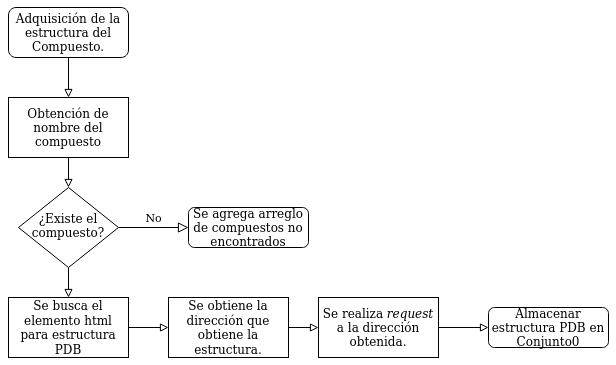
\includegraphics[scale=0.70]{Capitulo4/Documentos/imagenes_entorno/figura_flujo.png}
    \caption{Diagrama de flujo de adquisición PDB del compuesto haciendo uso de Web Scrapping.}
    \label{Diagrama_de_flujo_1}
\end{figure}

\noindent Junto con la estructura, la bio-actividad se adquiere por medio de  Drugbank y haciendo uso del Web Scrapping, una vez que se cuenta con el nombre del compuesto, se busca la sección de Actividad Biológica, para esto  de igual forma, ya se debe haber confirmado en el mismo proceso si el compuesto  existe. si en la página que muestra toda la información del compuesto, no se halla la sección deseada, se indica en  el archivo del conjunto 0 que no posee actividad, de existir la sección, se obtiene el contenido de la tabla, se realiza la conversión a una cadena de caracteres para ser guardada en el archivo  conjunto 0.

\begin{figure}[H]
    \centering
    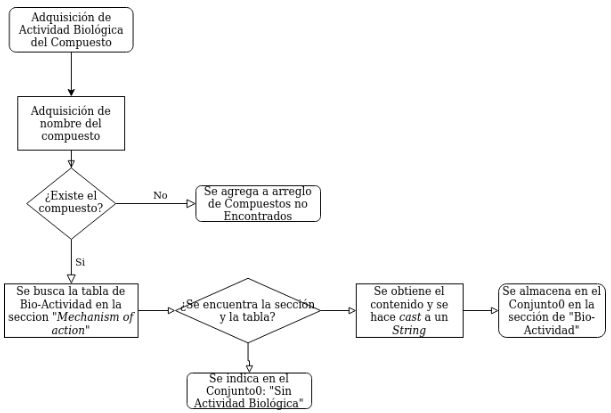
\includegraphics[scale=0.70]{Capitulo4/Documentos/imagenes_entorno/Actividad_biologica.png}
    \caption{Diagrama de flujo de adquisición de la Actividad Biológica}
    \label{Actividad_biologica}
\end{figure}

%%%%%%%%%%%%%%%%%%%%%%%%%%%%%%%%%%%%%%%%%%%%%%%%%%%%%%%%5
\subsubsection{Búsqueda concurrente}\label{concurrente}
\noindent El proceso de solicitar información a las API o realizar web scrapping, si bien no es complejo puede llegar a tomar algo de tiempo para recibir una respuesta del servidor que tienen las bases de datos. Para solucionar esta situación se utiliza la programación concurrente con hilos, los cuales evitan la latencia provocada por los tiempos que demoran las API en resolver las solicitudes que envía SisPAF. El programa crea un hilo por cada elemento que se obtuvo con la lectura del archivo inicial (tanto de compuestos como de proteínas). Cada hilo entonces tiene un elemento asociado del cual debe conseguir información mediante las peticiones a las API o el uso de web scrapping. Así, el tiempo requerido para realizar la búsqueda de información se reduce considerablemente.

\subsubsection{Construcción de conjuntos}
\noindent A la par de la actividad de búsqueda, una vez que la información es obtenida mediante las API’s, los hilos proceden a escribir esa información en archivos de texto. Para los compuestos, los hilos escriben la información en archivos de texto plano dentro de un directorio denominado Compounds, el cual está en el directorio donde se ha creado (o donde ya existe) el proyecto. Por su parte, la información de las proteínas es almacenada de la misma forma, solo que en un directorio de nombre Proteins. Los archivos que comprende el directorio Compounds forman el conjunto 0 (Véase \ref{diccionario}), mientras que todos los archivos que se encuentran en el directorio de Proteins forman el conjunto P (véase \ref{diccionario}).

\subsubsection{Manejo de pérdida de conexión a internet}
\noindent El manejo del error de conexión a internet está compuesto por tres partes. La primera parte es la detección de desconexión, que se realiza cuando alguna de las API’s o el proceso de webscrapping arrojan un error que se identifica como error de red. La segunda parte que toma lugar luego de que el error de red es identificado, es la de alerta al usuario de que no hay conexión a internet a la vez que se suspende el proceso de búsqueda, es decir, mientras no haya conexión las peticiones a las API’s y el webscrapping no son realizados pues los hilos se encuentran “dormidos”. La tercera parte es la reconexión la cual sucede cuando el usuario atiende la alerta emitida por el sistema, el cual como respuesta, realiza una rápida comprobación verificando si le es posible acceder al servidor central de Google. En caso de que le sea posible, el sistema emite una notificación para que todos los hilos que se encontraban pausados continúen con el proceso de la búsqueda de datos. Si por el contrario no es posible realizar la conexión al servidor de Google, la alerta vuelve a aparecer y el proceso de búsqueda se mantiene suspendido. La figura \ref{Desconexion} muestra el diagrama de flujo que sirvió como base para implementar la solución descrita en este apartado.

\begin{figure}[H]
    \centering
    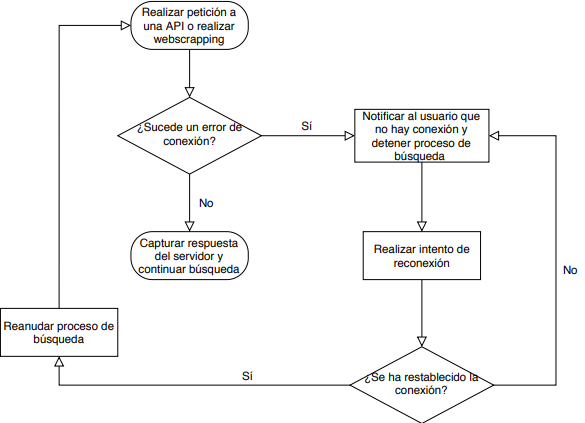
\includegraphics[scale=0.7]{Capitulo4/imagenes/diagramaDesconexion.png}
    \caption{Diagrama de flujo para el manejo de la pérdida de conexión a internet}
    \label{Desconexion}
\end{figure}

\subsubsection{Lectura de contenido de un proyecto}
\noindent Para el caso en el que el usuario desea abrir un proyecto ya existente, SisPAF solicita primero que se le indique el directorio donde se encuentra el proyecto. Acto seguido analiza la estructura de ese directorio para revisar que contenga los archivos que deben estar ahí puesto que si ya se ha creado un proyecto en ese directorio, deben existir ahí por lo menos el directorio de Compounds, el de Proteins y la copia del archivo inicial que genera el sistema (estos elementos se generan cuando se crea un nuevo proyecto). Si existen estos elementos procede a analizar el contenido de dichos directorios para determinar qué archivos faltan y que archivos se encuentran incompletos y requieren más información (esta lectura se realiza utilizando hilos para optimizar la tarea de leer varios archivos, se sigue la idea descrita en el apartado \ref{concurrente}). Una vez hecho esto se procede a continuar con el proceso ya sea de búsqueda o análisis dependiendo de la robustez actual del proyecto en cuestión. Si el sistema detecta un archivo final (Tabla \ref{diccionario}) no procede a abrir dicho proyecto pues este archivo es la muestra de que el proyecto ya ha sido terminado. La figura \ref{abrir} describe el diagrama de flujo que sigue el proceso de abrir un proyecto existente.

\begin{figure}[H]
    \centering
    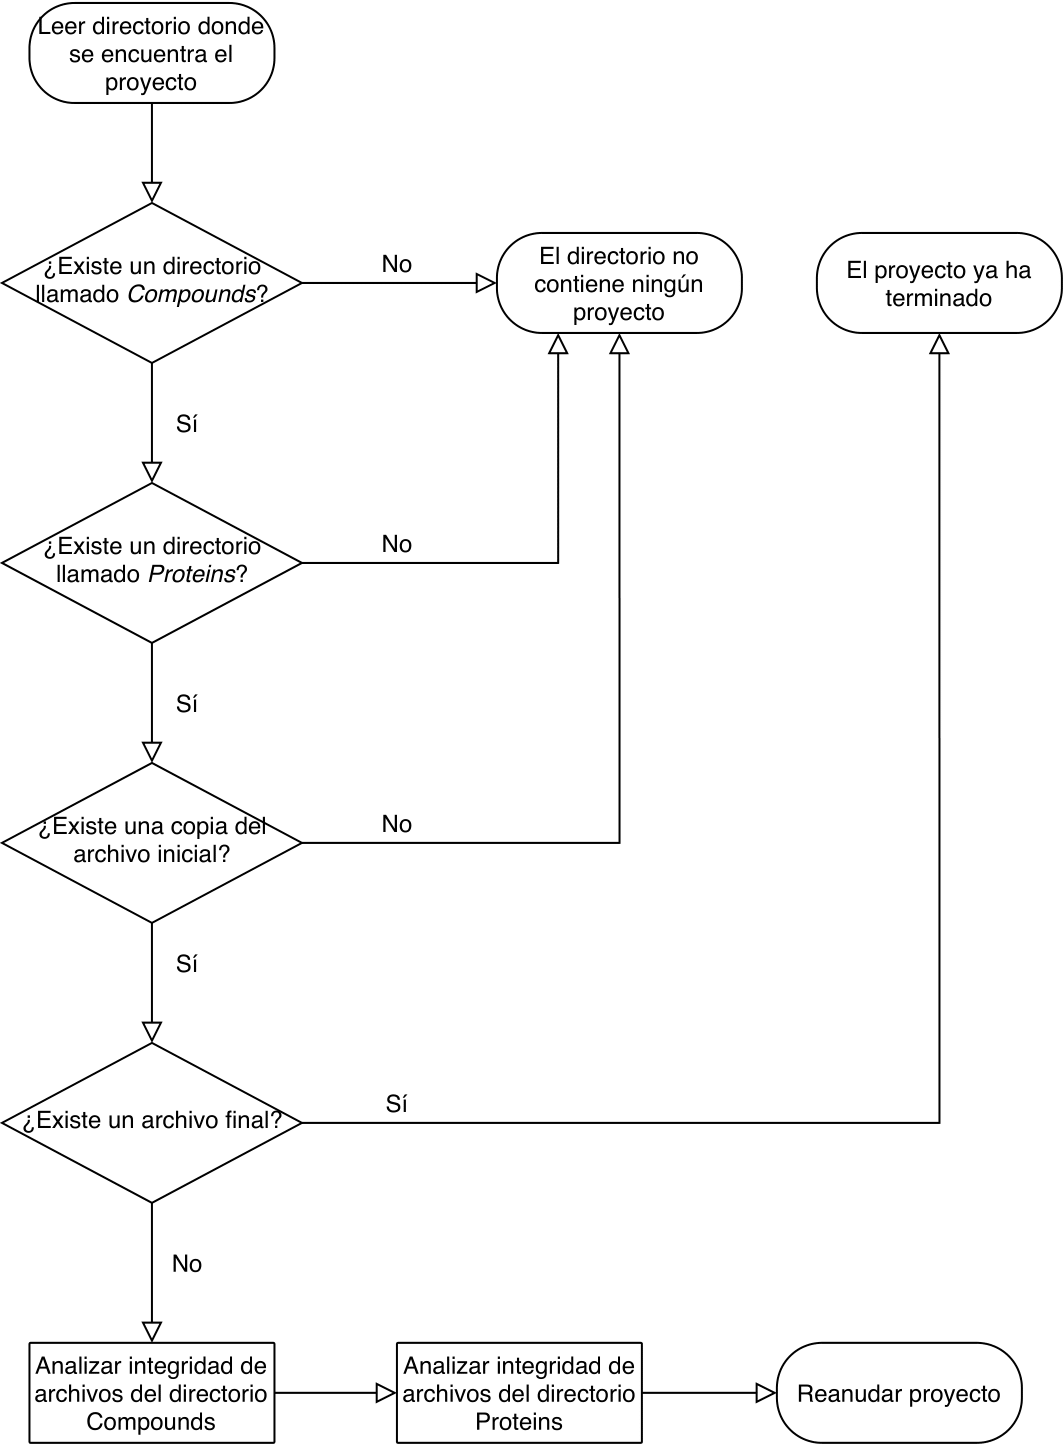
\includegraphics[scale=0.3]{Capitulo4/imagenes/diagramaAbrirProy-1.png}
    \caption{Diagrama de flujo que sigue SisPAF cuando se solicita abrir un proyecto ya existente.}
    \label{abrir}
\end{figure}
%%%%%%%%%%%%%%%%%%%%%%%%%%%%%%%%%%%%%%%%%%%%%%%%%%%%%
\subsection{Análisis de información}
\subsubsection{Diseño de interfaces}{
\noindent En la sección de análisis, donde el sistema hace uso de toda la información recolectada, se planificó una interfaz muy similar a la que se muestra durante el proceso de la búsqueda de información, una pantalla de espera,  para hacerle saber al usuario que el sistema  continúa trabajando, la comparación se muestra a continuación.

\begin{figure}[H]
    \centering
    \includegraphics[scale=0.27]{Capitulo4/Documentos/imagenes_generacion/Analisis.png}
    \caption{Comparación de pantallas para el análisis de datos, a la izquierda la planeada y a la derecha la programada.}
    \label{comparacion_6l}
\end{figure}
}
\subsubsection{Análisis multiproceso}{
\noindent El desarrollo del proceso del análisis de la información es considerado exhaustivo de CPU, es decir, este proceso requiere una considerable capacidad de procesamiento del equipo de cómputo. Contrario a la aplicación concurrente con hilos, para los procesos que involucran en uso considerable de recursos de procesamiento se emplea el método de multiprocesos. El uso de múltiples procesos para el módulo de análisis de información supone una reducción considerable en los tiempos de procesamiento. Aquí se toman en cuenta dos cosas, la primera es la cantidad de procesos y la división de tareas, ya que el número de procesos que se debe crear corresponde con el número de núcleos físicos del equipo de cómputo, y a su vez las tareas a realizar deben asignarse a cada uno de los procesos creados. La segunda cosa a tomar en cuenta es la ventaja de un trabajo en paralelo. El uso de múltiples procesos permite una paralelización de las actividades que debe realizar el sistema, es decir, si se tienen 4 núcleos, se pueden realizar al mismo tiempo (de manera paralela) 4 actividades, aprovechando al 100\% la capacidad de procesamiento del equipo de cómputo donde se está ejecutando el sistema.



}
\subsubsection{\textit{Docking}}{
\noindent En el campo de modelado molecular (acoplamiento molecular) es un método que predice la conformación preferida de una molécula, al estar unida a otra, con el fin de formar un complejo estable.\cite{15}\\
\noindent La simulación de este procedimiento es un proceso complicado. En este enfoque, la proteína y el ligando están separados por una distancia física, y el ligando encuentra su posición en el sitio activo de la proteína luego de un cierto número de ''movimientos'' en su espacio conformacional. Los movimientos incorporan al cuerpo rígido transformaciones tales como el traslado y rotaciones. Cada uno de estos movimientos, en el espacio conformacional del ligando, induce un costo energético al sistema, y por tanto después de cada movimiento, se calcula la energía total del sistema.\\

\noindent Para hacer un examen de acoplamiento, primero se necesita la estructura de la proteína. Normalmente la estructura ha sido determinada usando una técnica biofísica como la cristalografía de rayos X, o menos frecuente, una Espectroscopia de resonancia magnética nuclear. La estructura de esta proteína y la de los ligandos potenciales sirven como los valores a ingresar en el programa que calcula el acoplamiento. El éxito del programa depende de dos factores: el algoritmo de búsqueda y la función de puntuación.\\

\noindent Para el acoplamiento molecular usamos una herramienta llamada AutoDock Vina la cual permite calcular de manera automática cada uno de estos movimientos. Para generar el resultado de \textit{Docking} con vina, pide como parámetros un archivo donde se configuran las entradas al sistemas y que esperas como salida del mismo, un ejemplo de este archivo, está ilustrado en la figura \ref{dock_ing}.\\

\noindent Como salida tendremos un archivo PDBQT el cual nos da el valor del acoplamiento molecular en distintas iteraciones, a estos valores los llamaremos “Deltas” los cuales son una pieza fundamental para implementar el algoritmo de regresión lineal, ya que estos datos se convertirán en nuestra variable dependiente.

\begin{figure}[H]
    \centering
    \includegraphics[scale=.99]{Capitulo4/Documentos/imagenes_entorno/archivo_entrada.png}
    \caption{Archivo de configuración para\textit{Docking}.}
    \label{dock_ing}
\end{figure}

\noindent Como podemos ver, Vina pide como parámetros de entrada la estructura 3D de un receptor (molécula que recibe, por lo normal es una proteína u otro biopolímero) y la estructura 3D del ligando (molécula que se enlaza al receptor. Por lo general son moléculas más pequeñas que el receptor, aunque también pueden ser otro biopolímero).\\

\noindent De igual manera Vina pide como parámetros el centro del receptor, estas coordenadas las podemos generar a través de una herramienta de MGLTools (mismo desarrollador de AutoDockTools) la cual se encuentra dentro del archivo “prepare\_gpf4.py”, esta biblioteca nos permite generar las coordenadas ideales del centro del receptor, las cuales son indispensables para generar el \textit{Docking}, para utilizar esta biblioteca debemos tener las estructuras 3D del receptor y ligando en formato PDBQT por lo cual debemos realizar una conversión de estas estructuras ya que SysPAF las obtiene pero en su formato PDB.\\

\noindent Para realizar esta conversión, es necesario usar la biblioteca de MGLTools la cual transforma la estructura de la proteína y la prepara para ser receptora, al igual que cambia el formato de PDB a PDBQT. Esta biblioteca la podemos encontrar dentro del archivo “prepare\_receptor.py” para el caso de la transformación de un receptor ya que si se desea convertir la estructura de un ligando (estructura de un compuesto en el caso de SysPAF) es necesario utilizar el archivo “prepare\_ligand.py”.\\

\noindent La figura \ref{flujo_dock} muestra el flujo que sigue SysPAF para realizar el proceso de \textit{Docking}.

\begin{figure}[H]
    \centering
    \includegraphics[scale=.65]{Capitulo4/Documentos/imagenes_entorno/docking-flujo.png}
    \caption{Flujo que sigue SysPAF para realizar el proceso de \textit{Docking}.}
    \label{flujo_dock}
\end{figure}

}

\subsubsection{Implementación de algoritmos de \textit{Machine Learning}}{
\noindent El uso de algoritmos de Machine Learning permite la generación de modelos para realizar cálculos más rápidos en términos de predicción de la efectividad de los compuestos de estudio.El uso de algoritmos de \textit{Machine Learning} permite la generación de modelos para realizar cálculos más rápidos. Los modelos se obtienen a partir de una regresión lineal múltiple que toma como variables independientes a los valores de las propiedades físicas y químicas de cada medicamento. La variable dependiente está definida por el valor de delta G obtenido del proceso del \textit{Docking}. Luego de obtener los coeficientes de la regresión lineal, estos son almacenados en un archivo el cual contiene todos los modelos para las distintas clasificaciones de medicamentos (cada clasificación constituye un modelo). Una vez definido el modelo, el proceso del \textit{Docking} y de la regresión lineal puede omitirse en caso de volver a tener que realizar un análisis de información en el cual, luego de revisar el archivo donde se almacenan los modelos, se encuentre el modelo para la clase de compuestos que se están analizando. La figura \ref{Machine} muestra una ilustración del proceso previamente descrito.

\begin{figure}[H]
    \centering
    \includegraphics[scale=0.70]{Capitulo4/Documentos/imagenes_entorno/regresion_lineal.png}
    \caption{Forma de implementar la regresión lineal y su relación con los resultados del \textit{Docking}.}
    \label{Machine}
\end{figure}
\noindent Una vez que la regresión lineal es finalizada, el sistema guarda dicho modelo en una carpeta el cual puede recuperar en caso de que se solicite analizar datos correspondientes a una clasificación que corresponda con algún modelo de regresión lineal existente. Al recuperar el modelo correspondiente, se puede simplemente realizar el proceso de predicción directa de la variable Y, dado que en ese modelo se observan ya los coeficientes y las variables independientes X que están determinadas por los descriptores del nuevo conjunto 0 a analizar.
}
\subsubsection{Precisión del modelo de regresión lineal generado}{
\noindent La evaluación de qué tan acertado es el modelo de regresión lineal que se genera luego de aplicar el algoritmo del mismo nombre se basa en la obtener y medir la influencia de los errores en la exactitud del modelo de regresión lineal. Estos errores, si bien se implementan de manera directa gracias a las herramientas de la biblioteca de python sklearn, requieren de su correcta comprensión para poder entender qué tan exacto es el modelo y por qué.\\
\noindent La estadística ha desarrollado medidas resumidas que toman la colección de residuos del modelo (valor actual - valor esperado) y los condensan en un solo valor que representa la capacidad predictiva del modelo implementado. De estas medidas se han considerado 3: Error Medio Absoluto (MAE, por sus siglas en inglés, Mean Absolute Error), Error Cuadrático Medio (MSE, por sus siglas en inglés, Mean Square Error) y Raíz del Error Cuadrático Medio (RMSE, por sus siglas en inglés, Root Mean Square Error).\cite{16}\\

\noindent El error medio absoluto se obtiene mediante la sumatoria de cada valor absoluto del residual (diferencia entre el valor predicho y el valor esperado), y luego dividiendo entre el número de muestras. Este error  se refiere a la media de los valores absolutos de cada error de predicción en todas las instancias del conjunto de datos de prueba.\\
\noindent Para el caso de error medio cuadrado permite determinar qué tan cerca está una línea de regresión de un conjunto de puntos. Lo hace tomando las distancias desde los puntos hasta la línea de regresión (estas distancias son los "errores") y cuadrándolos. La cuadratura es necesaria para eliminar cualquier signo negativo. También le da más peso a las diferencias más grandes (outliers).\\

\noindent Por último, considerando que el error cuadrático medio es la desviación estándar de los residuos y sabiendo que los residuos son una medida de qué tan lejos están los puntos de datos de la línea de regresión, la raíz del error cuadrático medio es una medida de la dispersión de estos residuos. En otras palabras, dice qué tan concentrados están los datos alrededor de la línea de regresión.\\

\begin{figure}[H]
    \centering
    \includegraphics[scale=0.85]{}
    \caption{Representación matemática del error medio absoluto.}
    \label{ecuaciones}
\end{figure}

\begin{figure}[H]
    \centering
    \includegraphics[scale=0.85]{}
    \caption{Representación matemática del error cuadrático medio.}
    \label{ecuaciones}
\end{figure}

\begin{figure}[H]
    \centering
    \includegraphics[scale=0.85]{}
    \caption{Representación matemática de la raíz del error cuadrático medio.}
    \label{ecuaciones}
\end{figure}

\noindent Los errores previamente definidos se utilizan con la observación de que a menor valor, mejor. Es decir, que estos 3 valores resulten en 0 indicaría que el modelo es perfecto. Las pruebas para obtener estos errores se realizaron con los conjuntos de datos indicados que en anexo X. Y en promedio, de X pruebas se obtuvieron los resultados que ilustra la tabla siguiente.



\begin{longtable}{|c|c|c|c|c|c|}
\caption{Resultados de las mediciones de errores realizadas..}\\ 
\hline
\multirow{}{}{\textbf{Clasificación} } & \multicolumn{2}{c|}{\textbf{Número de muestras} } & \multirow{}{}{\textbf{MAE} } & \multirow{}{}{\textbf{MSE} } & \multirow{}{}{\textbf{RMSE} }  \\* 
\cline{2-3}
                                         & \textbf{Entrenamiento} & \textbf{Prueba}          &                                &                                &                                  \endfirsthead 
\hline
Anti-inflamatorio                        & 12                     & 4                        & 0.471                          & 0.472                          & 0.687                            \\ 
\hline
Antiviral                                & 4                      & 2                        & 2.583                          & 6.673                          & 2.583                            \\ 
\hline
Antiandrogénico                          & 2                      & 1                        & 0.82                           & 0.67                           & 0.82                             \\ 
\hline
Cardiovascular                           & 6                      & 2                        & 6.903                          & 72.383                         & 8.507                            \\ 
\hline
Antifúngico                              & 5                      & 2                        & 6.230                          & 39.48                          & 6.272                            \\ 
\hline
Antihipertensivo                         & 18                     & 5                        & 4.934                          & 39.784                         & 6.307                            \\ 
\hline
Antiparasitario                          & 7                      & 2                        & 0.46                           & 0.313                          & 0.56                             \\ 
\hline
Antibiótico                              & 4                      & 2                        & 2.353                          & 10.124                         & 3.181                            \\ 
\hline
Antiepiléptico                           & 5                      & 2                        & 0.03                           & 0.001                          & 0.032                            \\ 
\hline
Anticoagulante                           & 5                      & 2                        & 0.334                          & 0.133                          & 0.364                            \\ 
\hline
\textbf{Total}                           & \textbf{68}            & \textbf{24}              & \textbf{2.511}                 & \textbf{17.003}                & \textbf{2.931}                   \\
\hline
\end{longtable}

\noindent De estos resultados se puede decir que el modelo generado tiene un margen de error de 2.5 unidades, esto es, la variación entre el valor que se espera obtener y el valor que puede predecir el modelo está definida en un rango de 0 a 2.5, y considerando la cantidad de pruebas, se puede concluir que el modelo es eficaz.\\

\noindent Algo muy importante que se debe mencionar es que el modelo de regresión lineal depende en gran medida de la calidad y la cantidad de datos proporcionados. Un modelo con muchas variables independientes para trabajar pero que son pobres en cuanto a la relación cualitativa de estas variables con las variables dependientes resultan en un modelo predictivo poco preciso, por otro lado un modelo donde las variables dependientes tengan mucha influencia en la variable dependiente además de grandes muestras de información para entrenar y probar el modelo derivan en la generación de un modelo más preciso y robusto.
}

%%%%%%%%%%%%%%%%%%%%%%%%%%%%%%%%%%%%%%%%%%%%%%%%%%%%%
\subsection{Generación de resultados}
\subsubsection{Diseño de interfaces}
\noindent La interfaz de despliegue de resultados fue desarrollada con la finalidad de que el usuario pueda visualizar los resultados obtenidos por el sistema, los resultados están desplegados en una tabla de dos columnas, la columna uno lleva por nombre “Compuesto”, donde se en-lista el nombre de cada compuesto, la columna dos tiene el nombre de “Efectividad”, esta muestra los efectos que tuvo el compuesto para “destruir” la proteína, está  representada numéricamente. 

\begin{figure}[H]
    \centering
    \includegraphics[scale=0.52]{Capitulo4/Documentos/imagenes_generacion/imagen-2-2-7-2.png}
    \caption{Despliegue de resultados.}
    \label{Des_Res}
\end{figure}

\noindent La columna “Efectividad” nos ayudará a ordenar los resultados, ya que se tomará el valor más alto y este será nuestro punto de partida para desplegar nuestros resultados de forma descendente.

\subsubsection{Ordenamiento de resultados:}
\noindent Para el ordenamiento de los resultados, utilizamos una estructura de datos llamada “diccionario” en python, dicha estructura soporta cualquier tipo de dato como enteros, cadenas, listas e incluso otras funciones. La ventaja de utilizar este tipo de estructura es el poder identificar cada elemento por una clave (key) ya que está dada por duplas.

\noindent Donde tomamos el nombre del compuesto como la llave de la dupla y la efectividad como el valor. Para acceder a cada uno de los valores del diccionario de datos, es necesario poner el nombre de la clave (compuesto), lo cual nos permite eliminar la redundancia de datos, ya que esta estructura no guarda datos duplicados.

\subsubsection{Construcción de archivo de resultados:}
\noindent La Para evitar una pérdida de datos, se definió una función que nos permite guardar los resultados obtenidos por el sistema en un archivo txt, dicho archivo se encuentra guardado en una carpeta que lleva por nombre “Resultados” y a su vez este lleva por nombre “Resultados\_Proyecto.txt”. El archivo contiene una estructura similar a la tabla que se muestra en la interfaz de despliegue de resultados y de igual manera está ordenada de mayor a menor efectividad.

\begin{figure}[H]
    \centering
    \includegraphics[scale=0.52]{Capitulo4/Documentos/imagenes_generacion/imagen-2-2-8-1.png}
    \caption{Ejemplo de archivo guardado.}
    \label{fig:my_label}
\end{figure}

\subsubsection{Alertas y errores:}
\noindent La interfaz de “despliegue de resultados” cuenta con dos tipos de alertas, las cuales se muestran al efectuar una interacción específica con el sistema, describiremos a continuación dichas alertas de manera individual:

\noindent\textit{Resultados guardados:}\\

\noindent El sistema SisPAF muestra una alerta, cuando el documento fue guardado correctamente, esta acción surge de dar clic en el botón “Guardar” de la interfaz. El objetivo principal de desarrollar esta funcionalidad es notificar al usuario que la acción que realizó fue efectuada con éxito.\\

\begin{figure}[H]
    \centering
    \includegraphics[scale=0.85]{Capitulo4/Documentos/imagenes_generacion/manual_3.png}
    \caption{Resultados guardados correctamente}
    \label{resultados_guard}
\end{figure}

\noindent \textit{Resultados no guardados:}\\

\noindent El sistema SisPAF muestra una alerta que nos permite decidir si seguir con la acción que el usuario seleccionó, dicha acción puede estar descrita por un cierre forzado del sistema, dar clic en el botón “Inicio” o seleccionar el botón de “Salir” que fue implementado en el sistema, todo esto antes de guardar el documento de resultados. El objetivo de esta notificación es poder alertar al usuario de que sus resultados no han sido guardados y de seguir con esta acción podrían perderse y tendrían que ser calculados nuevamente.

\begin{figure}[H]
    \centering
    \includegraphics[scale=0.85]{Capitulo4/Documentos/imagenes_generacion/manual_4.png}
    \caption{Alerta de acción.}
    \label{resultados_guard}
\end{figure}

%%%%%%%%%%%%%%%%%%%%%%%%%%%%%%%%%%%%%%%%%
\section{Ejecución de las Pruebas Unitarias}

%%%%%%%%%%%%%%%%%%%%%%%%%%%%%%%%%%%%%%%%%%%%
%% Please add the following required packages to your document preamble:
% \usepackage{longtable}
% Note: It may be necessary to compile the document several times to get a multi-page table to line up properly
\begin{longtable}{|l|l|}
\caption{Prueba unitaria RF1.1}
\label{PU_RF1_1}\\
\hline

\textbf{Requerimiento Funcional}                                                       & \textbf{RF1.1 Adquisición del archivo base.}                                                                                                                                                                                                                                                                                                                                                                                                                                                                                                                                                                                                                                                     \\ \hline
\endfirsthead
%
\multicolumn{2}{c}%
{{\bfseries Tabla \thetable\ Continuación de la página anterior}} \\
\endhead
%
\textbf{Perfiles Implicados}                                                           & \begin{tabular}[c]{@{}l@{}}- Desarrollador.\\ - Tester.\end{tabular}                                                                                                                                                                                                                                                                                                                                                                                                                                                                                                                                                                                                                             \\ \hline
\textbf{Planificación temporal}                                                        & \begin{tabular}[c]{@{}l@{}}1. Prueba de compilación.\\ 2. Prueba de funcionamiento.\\ 2.1 Func. botón adquisición archivo.\\ 2.2 Muestra de pantalla selección de\\ archivo.\\ 2.3 Acceso a directorio.\\ 2.4 Carga de archivo.\\ 2.5 Func. botón buscar.\end{tabular}                                                                                                                                                                                                                                                                                                                                                                                                                           \\ \hline
\textbf{Criterio de verificación}                                                      & \begin{tabular}[c]{@{}l@{}}1. Compilación del código.\\ 2. Ejecutable del módulo, hay muestras\\ de que el código hace algo (algo: definido por los \\ siguientes puntos).\\ 2.1 Funcionamiento del botón de Archivo base.\\ 2.2 Visualización de selección de archivo.\\ 2.3 Acceso al directorio correcto o permite acceder \\ a uno distinto desde la pantalla de selección de \\ archivo.\\ 2.4 Carga del archivo correcto.\\ 2.5 El botón se ve adecuadamente y accede al\\ archivo indicado y logra una lectura correcta.\end{tabular}                                                                                                                                                     \\ \hline
\textbf{Criterio de aceptación}                                                        & \begin{tabular}[c]{@{}l@{}}1. No hay errores que impidan la compilación \\ del código.\\ 2. Al usar el ejecutable del módulo, hay muestras \\ de que el código hace algo \\ (algo: definido por los siguientes puntos).\\ 2.1 Se muestra el botón correspondiente, y realiza la \\ acción indicada.\\ 2.2 Es visualizada la pantalla de selección de archivos \\ con cada uno de los componentes.\\ 2.3 La selección de archivos se encuentra en el \\ directorio correcto o permite acceder a uno distinto.\\ 2.4 Solo permite la carga de un archivo de texto \\ plano, y es cargado adecuadamente.\\ 2.5 El botón se ve adecuada, y realiza la acción \\ indicada correctamente.\end{tabular} \\ \hline
\textbf{\begin{tabular}[c]{@{}l@{}}Definición de\\ verificaciones\end{tabular}}        & \begin{tabular}[c]{@{}l@{}}- Errores de Compilación: Ocurren porque la sintaxis \\ del lenguaje no es correcta, de cajón este tipo de \\ errores no permiten que la aplicación se ejecute. \\ \\ - Acción de botón: representa un botón que, cuando \\ es presionado, envía información al que pertenece. \\ La función de  un botón representada  el contenido\\ del elemento.\\ \\ -Visualización de pantalla interfaz de usuario.\end{tabular}                                                                                                                                                                                                                                                \\ \hline
\textbf{\begin{tabular}[c]{@{}l@{}}Análisis y evaluación\\ de resultados\end{tabular}} &                                                                                                                                                                                                                                                                                                                                                                                                                                                                                                                                                                                                                                                                                                  \\ \hline
\textbf{Productos  a entregar}                                                         & \begin{tabular}[c]{@{}l@{}}- Adquisición del archivo base funcionando \\ correctamente.\end{tabular}                                                                                                                                                                                                                                                                                                                                                                                                                                                                                                                                                                                             \\ \hline

\end{longtable}
% Please add the following required packages to your document preamble:
% \usepackage{longtable}
% Note: It may be necessary to compile the document several times to get a multi-page table to line up properly
\begin{longtable}{|l|l|}
\caption{Caso de prueba RF1}
\label{CP_RF1}\\
\hline
\textbf{ID del Caso de prueba}                                                          & CPRF1                                                                                                                                                            \\ \hline
\endfirsthead
%
\multicolumn{2}{c}%
{{\bfseries Tabla \thetable\ Continuación de la página anterior}} \\
\endhead
%
\textbf{Versión}                                                                        & 1.0                                                                                                                                                              \\ \hline
\textbf{Nombre}                                                                         & Caso de prueba para adquisición de archivo base.                                                                                                                 \\ \hline
\textbf{\begin{tabular}[c]{@{}l@{}}Identificador de \\ requerimiento\end{tabular}}      & RF1.1                                                                                                                                                            \\ \hline
\textbf{Propósito}                                                                      & \begin{tabular}[c]{@{}l@{}}Determinar capacidad del sistema para \\ obtener el archivo base.\end{tabular}                                                        \\ \hline
\textbf{Dependencias}                                                                   & N/A                                                                                                                                                              \\ \hline
\textbf{\begin{tabular}[c]{@{}l@{}}Ambiente de \\ prueba/configuración\end{tabular}}    & \begin{tabular}[c]{@{}l@{}}- Hardware: Equipo de computo\\ (preferentemente portatíl)\\ - Software: Compilador python3, \\ IDE y/o editor de texto.\end{tabular} \\ \hline
\textbf{Inicialización}                                                                 & \begin{tabular}[c]{@{}l@{}}- Codificación correspondiente al \\ requerimiento.\\ - Creación del archivo base.\end{tabular}                                       \\ \hline
\textbf{Finalización}                                                                   & N/A                                                                                                                                                              \\ \hline
\textbf{Acciones}                                                                       & \begin{tabular}[c]{@{}l@{}}. Compilar el código correspondiente.\\ - Colocar el archivo en el directorio \\ especificado.\end{tabular}                           \\ \hline
\textbf{\begin{tabular}[c]{@{}l@{}}Descripción de los \\ datos de entrada\end{tabular}} & \begin{tabular}[c]{@{}l@{}}- Archivo de texto plano.\\ - Directorio de la ubicación del archivo base.\end{tabular}                                               \\ \hline
\textbf{Salida esperada}                                                                & \begin{tabular}[c]{@{}l@{}}- Notificación de adecuada adquisición del \\ archivo base.\end{tabular}                                                              \\ \hline
\textbf{Salida obtenida}                                                                &  \begin{tabular}[c]{@{}l@{}}- Cuadro de diálogo para la obtención de archivos.\\
- Diálogo para indicar que un archivo es incorrecto.\\
- Sin diálogo para cuando el archivo es correcto;\\ Se sustituye por la habilitación de botón de inicio.\end{tabular}                                                                                                                                              
\\ \hline
\textbf{Resultado}                                                                      & \begin{tabular}[c]{@{}l@{}}- El módulo funciona adecuadamente,
aparecen los \\diálogos necesarios para la
interpretación  del usuario.\end{tabular}                                                                                                                                               
\\ \hline
\textbf{Severidad}                                                                      & - Baja                                                                                                                                                      \\ \hline
\textbf{Evidencia}                                                                      &   \begin{tabular}[c]{@{}l@{}} Evidencia en la imagen \ref{CPRF1}.\end{tabular}                                                                                                                                                            \\ \hline
\textbf{Estado}                                                                         & Iniciado                                                                                                                                                    \\ \hline
\end{longtable}
%%%%%%%%%%%%%%%%%%%%%%%%%%%%%%%%%%%%%%%%%%%%
%% Please add the following required packages to your document preamble:
% \usepackage{longtable}
% Note: It may be necessary to compile the document several times to get a multi-page table to line up properly
\begin{longtable}{|l|l|}
\caption{Prueba unitaria RF1.2}
\label{PU_RF1_2}\\
\hline
\textbf{Requerimiento Funcional}                                                       & \textbf{RF1.2 Búsqueda de los compuestos indicados..}                                                                                                                                                                                                                                                                                                                                                                                                                                                                                                                                  \\ \hline
\endfirsthead
%
\multicolumn{2}{c}%
{{\bfseries Table \thetable\ Continuación de la página anterior}} \\
\endhead
%
\textbf{Perfiles Implicados}                                                           & \begin{tabular}[c]{@{}l@{}}- Desarrollador.\\ - Tester.\end{tabular}                                                                                                                                                                                                                                                                                                                                                                                                                                                                                                                   \\ \hline
\textbf{Planificación temporal}                                                        & \begin{tabular}[c]{@{}l@{}}1. Prueba de compilación.\\ 2. Prueba de funcionamiento.\\ 2.1 Verificar adecuada lectura del archivo base\\ (token “compunds” ).\\ 2.2 Comprobar conexión a la base de datos \\ “DrugBank”.\\ 2.3 Obtención del .pdb de cada uno de los \\ compuestos enlistados.\\ 2.4 Almacenado del .pdb en el sistema.\end{tabular}                                                                                                                                                                                                                                   \\ \hline
\textbf{Criterio de verificación}                                                      & \begin{tabular}[c]{@{}l@{}}1. Compilación del código.\\ 2. Ejecutable del módulo, hay muestras de que el \\ código hace algo\\ (algo: definido por los siguientes puntos).\\ 2.1 Lectura del token que describe los nombres del\\ compuesto en el archivo base.\\ 2.2 Conexión a  DrugBank y por lo tanto a Internet.\\ 2.3 Adquirir el archivo .pdb del compuesto correcto.\\ 2.4 Almacenamiento de un archivo íntegro en el \\ sistema.\end{tabular}                                                                                                                                \\ \hline
\textbf{Criterio de aceptación}                                                        & \begin{tabular}[c]{@{}l@{}}1. No hay errores que impidan la compilación del \\ código.\\ 2. Al usar el ejecutable del módulo, hay muestras \\ de que el código hace algo\\ (algo: definido por los siguientes puntos).\\ 2.1 No se pierde ningún valor ni dato existente en el\\ archivo base.\\ 2.2 El sistema informa la correcta conexión a \\ “DrugBank”.\\ 2.3 El sistema informa que el compuesto existe \\ en la base de datos y confirma la adquisición \\ del .pdb.\\ 2.4 El sistema notifica la correcta obtención del \\ archivo .pdb y correcto  almacenado.\end{tabular} \\ \hline
\textbf{\begin{tabular}[c]{@{}l@{}}Definición de\\ verificaciones\end{tabular}}        & \begin{tabular}[c]{@{}l@{}}- Errores de Compilación: Ocurren porque la sintaxis \\ del lenguaje no es correcta, de cajón este tipo de \\ errores no permiten que la aplicación se ejecute. \\ \\ - Conexión a base de datos online:Una conexión a \\ base de datos es un archivo de configuración donde \\ se especifica los detalles físicos de una base de datos \\ como por ejemplo el tipo de base de datos y la \\ versión, y los parámetros que permiten una conexión\end{tabular}                                                                                               \\ \hline
\textbf{\begin{tabular}[c]{@{}l@{}}Análisis y evaluación\\ de resultados\end{tabular}} &                                                                                                                                                                                                                                                                                                                                                                                                                                                                                                                                                                                        \\ \hline
\textbf{Productos  a entregar}                                                         & \begin{tabular}[c]{@{}l@{}}- Búsqueda de los compuestos indicados \\ funcionando correctamente.\end{tabular}                                                                                                                                                                                                                                                                                                                                                                                                                                                                           \\ \hline
\end{longtable}
% Please add the following required packages to your document preamble:
% \usepackage{longtable}
% Note: It may be necessary to compile the document several times to get a multi-page table to line up properly
\begin{longtable}{|l|l|}
\caption{Caso de prueba RF1.2}
\label{CP_RF1_2}\\
\hline
\textbf{ID del Caso de prueba}                                                          & CPRF2                                                                                                                                                                                                                                        \\ \hline
\endfirsthead
%
\multicolumn{2}{c}%
{{\bfseries Tabla \thetable\ Continuación de la página anterior}} \\
\endhead
%
\textbf{Versión}                                                                        & 1.0                                                                                                                                                                                                                                          \\ \hline
\textbf{Nombre}                                                                         & \begin{tabular}[c]{@{}l@{}}Caso de prueba para la búsqueda de los \\ compuestos indicados.\end{tabular}                                                                                                                                      \\ \hline
\textbf{\begin{tabular}[c]{@{}l@{}}Identificador de \\ requerimiento\end{tabular}}      & RF1.2                                                                                                                                                                                                                                        \\ \hline
\textbf{Propósito}                                                                      & \begin{tabular}[c]{@{}l@{}}Calificar la búsqueda del compuesto en la base \\ de datos “Drug Bank” , desde obtener el nombre \\ en el archivo base a la adquisición del .pdb.\end{tabular}                                                  \\ \hline
\textbf{Dependencias}                                                                   & Correcta obtención del archivo base.                                                                                                                                                                                                         \\ \hline
\textbf{\begin{tabular}[c]{@{}l@{}}Ambiente de \\ prueba/configuración\end{tabular}}    & \begin{tabular}[c]{@{}l@{}}- Hardware: Equipo de computo\\ (preferentemente portatíl)\\ - Software: Compilador python3, \\ IDE y/o editor de texto.\end{tabular}                                                                             \\ \hline
\textbf{Inicialización}                                                                 & \begin{tabular}[c]{@{}l@{}}- Codificación correspondiente al \\ requerimiento.\\ - Creación del archivo base.\end{tabular}                                                                                                                   \\ \hline
\textbf{Finalización}                                                                   & N/A                                                                                                                                                                                                                                          \\ \hline
\textbf{Acciones}                                                                       & \begin{tabular}[c]{@{}l@{}}. Compilar el código correspondiente.\\ - Contar con el archivo base previamente \\ cargado.\end{tabular}                                                                                                         \\ \hline
\textbf{\begin{tabular}[c]{@{}l@{}}Descripción de los \\ datos de entrada\end{tabular}} & \begin{tabular}[c]{@{}l@{}}- Archivo de texto plano.\\ - Dirección para la conexión a “Drug Bank”.\end{tabular}                                                                                                                              \\ \hline
\textbf{Salida esperada}                                                                & \begin{tabular}[c]{@{}l@{}}Notificación de adecuada estado del \\ compuesto en “Drug Bank” (Existente o no).\\ - De existir, informar que el compuesto \\ existe al igual que el archivo .pdb\\ - Adquisición correcta del .pdb\end{tabular} \\ \hline
\textbf{Salida obtenida}                                                                &    \begin{tabular}[c]{@{}l@{}}- La notificación de la obtención de resultados\\ se realiza al finalizar toda la búsqueda de \\información necesaria.\\
- En la terminal se muestra el avance que se \\lleva con la búsqueda.
\end{tabular}                                                                                                                                                                                                                                         \\ \hline
\textbf{Resultado}                                                                      &     \begin{tabular}[c]{@{}l@{}}- Muestra de avance de la búsqueda general, \\por terminal y por medio de la interfaz,\\ a través de una barra de proceso.
\end{tabular}                                                                                                                                                                                                                                           \\ \hline
\textbf{Severidad}                                                                      &  Baja                                                                                                                                                                                                                                            \\ \hline
\textbf{Evidencia}                                                                      &   Evidencia en la imagen \ref{CPRF2-3-4}                                                                                                                                                                                                                                           \\ \hline
\textbf{Estado}                                                                         & Iniciado.                                                                                                                                                                                                                                 \\ \hline
\end{longtable}
%%%%%%%%%%%%%%%%%%%%%%%%%%%%%%%%%%%%%%%%%%%%
%% Please add the following required packages to your document preamble:
% \usepackage{longtable}
% Note: It may be necessary to compile the document several times to get a multi-page table to line up properly
\begin{longtable}{|l|l|}
\caption{Prueba unitaria RF1.3}
\label{PU_RF1_3}\\
\hline
\textbf{Requerimiento Funcional}                                                       & \textbf{\begin{tabular}[c]{@{}l@{}}RF1.3 Búsqueda de los descriptores de los \\ compuestos.\end{tabular}}                                                                                                                                                                                                                                                                                                                                                                                                                                                                                                                                                                                                                                                                                                                                                                                      \\ \hline
\endfirsthead
%
\multicolumn{2}{c}%
{{\bfseries Tabla \thetable\ Continuación de la página anterior}} \\
\endhead
%
\textbf{Perfiles Implicados}                                                           & \begin{tabular}[c]{@{}l@{}}- Desarrollador.\\ - Tester.\end{tabular}                                                                                                                                                                                                                                                                                                                                                                                                                                                                                                                                                                                                                                                                                                                                                                                                                           \\ \hline
\textbf{Planificación temporal}                                                        & \begin{tabular}[c]{@{}l@{}}1. Prueba de compilación.\\ 2. Prueba de funcionamiento.\\ 2.1 Verificar que el sistema mantiene el nombre \\ del compuesto sobre del que están obteniendo \\ los datos.\\ 2.2 Comprobar conexión a la base de datos \\ “ChemSpider” y “PubChem”.\\ 2.3 Búsqueda del compuesto en las bases de \\ datos.\\ 2.3.1  Existe el compuesto con el nombre \\ exacto en “PubChem”. \\ 2.3.2 Existe el compuesto con el nombre \\ exacto en “ChemSpider”.\\ 2.4 Adquisición de los descriptores del \\ compuesto en las bases de datos.\\ 2.3.1  Se adquieren  los descriptores  existentes en \\ “PubChem” del compuesto. \\ 2.3.2 Se adquieren  los descriptores  existentes en \\ “ChemSpider” del compuesto.\\ 2.4 Creación del archivo “Descriptors”.\\ 2.5 Almacenado de los datos adquiridos en \\ el archivo correspondiente , recientemente creado.\end{tabular} \\ \hline
\textbf{Criterio de verificación}                                                      & \begin{tabular}[c]{@{}l@{}}1. Compilación del código.\\ 2. Ejecutable del módulo, hay muestras de que el \\ código hace algo\\ (algo: definido por los siguientes puntos).\\ 2.1Verificación de integridad de la variable que \\ contiene el nombre del compuesto.\\ 2.2 Conexión a  “ChemSpider” y “PubChem” \\ y por lo tanto a Internet.\\ 2.3 Adecuada búsqueda del del compuesto exacto \\ en la base de datos.\\ 2.3.1 Correcta adquisición de los descriptores en\\ “PubChem”.\\ 2.3.2 Correcta adquisición de los descriptores en\\ “ChemSpider”.\\ 2.4 Creación del archivo “Descriptors” \\ correspondiente con el compuesto.\\ 2.5 Corroborar guardado de la información \\ obtenida en el archivo creado.\end{tabular}                                                                                                                                                          \\ \hline
\textbf{Criterio de aceptación}                                                        & \begin{tabular}[c]{@{}l@{}}1. No hay errores que impidan la compilación \\ del código.\\ 2. Al usar el ejecutable del módulo, hay muestras \\ de que el código hace algo\\ (algo: definido por los siguientes puntos).\\ 2.1 No se distorsiona el nombre del compuesto \\ de interés.\\ 2.2 El sistema informa la correcta conexión a\\ “ChemSpider”.\\ 2.3 El sistema informa la correcta conexión a \\ “PubChem”.\\ 2.4 El sistema informa que el mismo compuesto \\ existe en ambos repositorios.\\ 2.5. Se notifica la adecuada obtención de los \\ descriptores del compuesto.\\ 2.6 El sistema informa la correcta creación del\\  archivo.\\ 2.7 El archivo y la información que contiene es \\ integra.\end{tabular}                                                                                                                                                                   \\ \hline
\textbf{\begin{tabular}[c]{@{}l@{}}Definición de\\ verificaciones\end{tabular}}        & \begin{tabular}[c]{@{}l@{}}- Errores de Compilación: Ocurren porque la \\ sintaxis del lenguaje no es correcta, de cajón \\ este tipo de errores no permiten que la \\ aplicación se ejecute. \\ \\ - Conexión a base de datos online: \\ Una conexión a base de datos es un archivo \\ de configuración donde se especifica los \\ detalles físicos de una base de datos como por \\ ejemplo el tipo de base de datos y la versión, y \\ los parámetros que permiten una conexión\end{tabular}                                                                                                                                                                                                                                                                                                                                                                                                \\ \hline
\textbf{\begin{tabular}[c]{@{}l@{}}Análisis y evaluación\\ de resultados\end{tabular}} & - Resultados:                                                                                                                                                                                                                                                                                                                                                                                                                                                                                                                                                                                                                                                                                                                                                                                                                                                                                  \\ \hline
\textbf{Productos  a entregar}                                                         & \begin{tabular}[c]{@{}l@{}}- Búsqueda de los descriptores correspondientes\\  al compuesto de interés.\end{tabular}                                                                                                                                                                                                                                                                                                                                                                                                                                                                                                                                                                                                                                                                                                                                                                            \\ \hline
\end{longtable}
% Please add the following required packages to your document preamble:
% \usepackage{longtable}
% Note: It may be necessary to compile the document several times to get a multi-page table to line up properly
\begin{longtable}{|l|l|}
\caption{Caso de prueba RF1.3}
\label{CP_RF1_3}\\
\hline
\textbf{ID del Caso de prueba}                                                          & CPRF3                                                                                                                                                                                                                                                          \\ \hline
\endfirsthead
%
\multicolumn{2}{c}%
{{\bfseries Tabla \thetable\ Continuación de la página anterior}} \\
\endhead
%
\textbf{Versión}                                                                        & 1.0                                                                                                                                                                                                                                                            \\ \hline
\textbf{Nombre}                                                                         & \begin{tabular}[c]{@{}l@{}}Caso de prueba para la búsqueda de los \\ descriptores de los compuestos.\end{tabular}                                                                                                                                              \\ \hline
\textbf{\begin{tabular}[c]{@{}l@{}}Identificador de \\ requerimiento\end{tabular}}      & RF1.3                                                                                                                                                                                                                                                          \\ \hline
\textbf{Propósito}                                                                      & \begin{tabular}[c]{@{}l@{}}Identificar el funcionamiento del sistema al \\ momento de conectarse a las dos bases de datos \\ contenedoras de descriptores de compuestos, \\ “ChemSpider” y “PubChem”.\end{tabular}                                             \\ \hline
\textbf{Dependencias}                                                                   & Correcta obtención del archivo base.                                                                                                                                                                                                                           \\ \hline
\textbf{\begin{tabular}[c]{@{}l@{}}Ambiente de \\ prueba/configuración\end{tabular}}    & \begin{tabular}[c]{@{}l@{}}- Hardware: Equipo de computo\\ (preferentemente portatíl)\\ - Software: Compilador python3, \\ IDE y/o editor de texto.\end{tabular}                                                                                               \\ \hline
\textbf{Inicialización}                                                                 & \begin{tabular}[c]{@{}l@{}}- Codificación correspondiente al \\ requerimiento.\\ - Creación del archivo base.\end{tabular}                                                                                                                                     \\ \hline
\textbf{Finalización}                                                                   & N/A                                                                                                                                                                                                                                                            \\ \hline
\textbf{Acciones}                                                                       & \begin{tabular}[c]{@{}l@{}}. Compilar el código correspondiente.\\ - Contar con el archivo base previamente \\ cargado.\end{tabular}                                                                                                                           \\ \hline
\textbf{\begin{tabular}[c]{@{}l@{}}Descripción de los \\ datos de entrada\end{tabular}} & \begin{tabular}[c]{@{}l@{}}- Nombre del compuesto.\\ - Dirección para la conexión a \\ “ChemSpider” y “PubChem”.\end{tabular}                                                                                                                                  \\ \hline
\textbf{Salida esperada}                                                                & \begin{tabular}[c]{@{}l@{}}- Notificación de adecuada estado del \\ compuesto en\\ “ChemSpider” y “PubChem”. (Existente o no).\\ - De existir, informar que el compuesto existe \\ al igual que el archivo .pdb\\ - Adquisición correcta del .pdb\end{tabular} \\ \hline
\textbf{Salida obtenida}                                                                &   \begin{tabular}[c]{@{}l@{}}- Se ha optado por únicamente valerse de \\los descriptores existentes en PubChem.\\
- La notificación de la obtención \\de resultados se realiza al finalizar toda \\la búsqueda de información necesaria.\\
- En la terminal se muestra el avance que \\se lleva con la búsqueda.
\end{tabular}                                                                                                                                                                                                                                             \\ \hline
\textbf{Resultado}                                                                      &   \begin{tabular}[c]{@{}l@{}}- Muestra de avance de la búsqueda general,\\ por terminal y por medio de la interfaz, \\a través de una barra de proceso.
\end{tabular}                                                                                                                                                                                                                                                             \\ \hline
\textbf{Severidad}                                                                      &    - Baja                                                                                                                                                                                                                                                            \\ \hline
\textbf{Evidencia}                                                                      &  Evidencia en la imagen \ref{CPRF2-3-4}                                                                                                                                                                                                                                                         \\ \hline
\textbf{Estado}                                                                         & Iniciado.                                                                                                                                                                                                                                                   \\ \hline
\end{longtable}
%%%%%%%%%%%%%%%%%%%%%%%%%%%%%%%%%%%%%%%%%%%%
%% Please add the following required packages to your document preamble:
% \usepackage{longtable}
% Note: It may be necessary to compile the document several times to get a multi-page table to line up properly
\begin{longtable}{|l|l|}
\caption{Prueba unitaria RF1.4}
\label{PU_RF1_4}\\
\hline
\textbf{Requerimiento Funcional}                                                       & \textbf{\begin{tabular}[c]{@{}l@{}}RF1.4 Búsqueda de los mecanismos de \\acción de los compuestos.\end{tabular}}                                                                                                                                                                                                                                                                                                                                                                                                                                                                                                                                                                                                                                                                                                         \\ \hline
\endfirsthead
%
\multicolumn{2}{c}%
{{\bfseries Tabla \thetable\ Continuación de la página anterior}} \\
\endhead
%
\textbf{Perfiles Implicados}                                                           & \begin{tabular}[c]{@{}l@{}}- Desarrollador.\\ - Tester.\end{tabular}                                                                                                                                                                                                                                                                                                                                                                                                                                                                                                                                                                                                                                                                                                                                                        \\ \hline
\textbf{Planificación temporal}                                                        & \begin{tabular}[c]{@{}l@{}}1. Prueba de compilación.\\ 2. Prueba de funcionamiento.\\ 2.1 Verificar que el sistema mantiene el nombre \\ del compuesto sobre del que están obteniendo \\ los datos.\\ 2.2 Comprobar estado de la conexión a la base \\ de datos “DrugBank”.\\ 2.3 Comprobar que se mantiene la dirección\\ correspondiente  a el compuesto sobre el que \\ se está trabajando.\\ 2.4 Adquisición de la representación cuantitativa  \\ de la actividad biológica del compuesto en la \\ bases de datos “DrugBank”. \\ 2.5 Creación del archivo “BioActivity”.\\ 2.6 Almacenado de los datos adquiridos en el \\ archivo correspondiente , recientemente creado.\end{tabular}                                                                                                                                \\ \hline
\textbf{Criterio de verificación}                                                      & \begin{tabular}[c]{@{}l@{}}1. Compilación del código.\\ 2. Ejecutable del módulo, hay muestras de que el \\ código hace algo\\ (algo: definido por los siguientes puntos).\\ 2.1Verificación de integridad de la variable que \\ contiene el nombre del compuesto.\\ 2.2 Conexión a  “DrugBank” y por lo tanto a \\ Internet.\\ 2.3 Adecuada búsqueda del compuesto exacto \\ en la base de datos.\\ 2.4 Correcta adquisición de las cantidades \\ descriptivas de la actividad biológica en \\ “DrugBank”.\\ 2.5 Creación del archivo “BioActivity” \\ correspondiente con el compuesto.\\ 2.6 Corroborar guardado de la información \\ obtenida en el archivo creado\end{tabular}                                                                                                                                       \\ \hline
\textbf{Criterio de aceptación}                                                        & \begin{tabular}[c]{@{}l@{}}1. No hay errores que impidan la compilación \\ del código.\\ 2. Al usar el ejecutable del módulo, hay \\ muestras de que el código hace algo\\ (algo: definido por los siguientes puntos).\\ 2.1 No se distorsiona el nombre del compuesto \\ de interés.\\ 2.2 El sistema informa la correcta conexión a \\ “DrugBank”.\\ 2.3. Se notifica la adecuada obtención de los \\ datos cuantitativos de la actividad biológica \\ del compuesto.\\ 2.4 El sistema informa la correcta creación \\ del archivo.\\ 2.5 Son guardados todos los datos obtenidos \\ de DrugBank en el archivo creado.\end{tabular}                                                                                                                                                                                       \\ \hline
\textbf{\begin{tabular}[c]{@{}l@{}}Definición de\\ verificaciones\end{tabular}}        & \begin{tabular}[c]{@{}l@{}}- Errores de Compilación: Ocurren porque \\ la sintaxis del lenguaje no es correcta, de \\ cajón este tipo de errores no permiten que \\ la aplicación se ejecute. \\ \\ - Conexión a base de datos online: Una conexión \\ a base de datos es un archivo de configuración \\ donde se especifica los detalles físicos de una \\ base de datos como por ejemplo el tipo de \\ base de datos y la versión, y los parámetros que \\ permiten una conexión.\\ \\ - Manejo de Archivos: Un programa no puede \\ manipular los datos de un archivo directamente. \\ Para usar un archivo, un programa siempre \\ abrir el archivo y asignarlo a una variable, que \\ llamaremos el archivo lógico. Todas las \\ operaciones sobre un archivo se realizan a través \\ del archivo lógico.\end{tabular} \\ \hline
\textbf{\begin{tabular}[c]{@{}l@{}}Análisis y evaluación\\ de resultados\end{tabular}} & - Resultados:                                                                                                                                                                                                                                                                                                                                                                                                                                                                                                                                                                                                                                                                                                                                                                                                               \\ \hline
\textbf{Productos  a entregar}                                                         & \begin{tabular}[c]{@{}l@{}}-Búsqueda de la actividad biológica del \\ compuesto de interés funcionando correctamente.\end{tabular}                                                                                                                                                                                                                                                                                                                                                                                                                                                                                                                                                                                                                                                                                          \\ \hline
\end{longtable}
% Please add the following required packages to your document preamble:
% \usepackage{longtable}
% Note: It may be necessary to compile the document several times to get a multi-page table to line up properly
\begin{longtable}{|l|l|}
\caption{Caso de prueba RF1.4}
\label{CP_RF_4}\\
\hline
\textbf{ID del Caso de prueba}                                                          & CPRF4                                                                                                                                                                                                                                                                                                                         \\ \hline
\endfirsthead
%
\multicolumn{2}{c}%
{{\bfseries Tabla \thetable\ Continuación de la página anterior}} \\
\endhead
%
\textbf{Versión}                                                                        & 1.0                                                                                                                                                                                                                                                                                                                           \\ \hline
\textbf{Nombre}                                                                         & \begin{tabular}[c]{@{}l@{}}Caso de prueba para la búsqueda de los \\ mecanismos de acción de los compuestos.\end{tabular}                                                                                                                                                                                                             \\ \hline
\textbf{\begin{tabular}[c]{@{}l@{}}Identificador de \\ requerimiento\end{tabular}}      & RF1.4                                                                                                                                                                                                                                                                                                                         \\ \hline
\textbf{Propósito}                                                                      & \begin{tabular}[c]{@{}l@{}}Identificar el funcionamiento del sistema al \\ momento de re-conectarse o mantenerse conectado\\ a la base de datos contenedora de los datos \\ cuantitativos representantes de la actividad \\ biológica de los compuestos, “DrugBank”.\end{tabular}                                            \\ \hline
\textbf{Dependencias}                                                                   & \begin{tabular}[c]{@{}l@{}}- Correcta obtención del archivo base.\\ - Correcta adquisición de la estructura molecular \\ del compuesto.\\ - Adecuada conexión de la base de datos \\ “DrugBank”.\end{tabular}                                                                                                                 \\ \hline
\textbf{\begin{tabular}[c]{@{}l@{}}Ambiente de \\ prueba/configuración\end{tabular}}    & \begin{tabular}[c]{@{}l@{}}- Hardware: Equipo de computo\\ (preferentemente portatíl)\\ - Software: Compilador python3, \\ IDE y/o editor de texto.\end{tabular}                                                                                                                                                              \\ \hline
\textbf{Inicialización}                                                                 & \begin{tabular}[c]{@{}l@{}}- Codificación correspondiente al \\ requerimiento.\\ - Creación del archivo base.\end{tabular}                                                                                                                                                                                                    \\ \hline
\textbf{Finalización}                                                                   & N/A                                                                                                                                                                                                                                                                                                                           \\ \hline
\textbf{Acciones}                                                                       & \begin{tabular}[c]{@{}l@{}}. Compilar el código correspondiente.\\ - Contar con el archivo base previamente \\ cargado.\end{tabular}                                                                                                                                                                                          \\ \hline
\textbf{\begin{tabular}[c]{@{}l@{}}Descripción de los \\ datos de entrada\end{tabular}} & \begin{tabular}[c]{@{}l@{}}- Nombre del compuesto.\\ - Dirección para la conexión a “DrugBank”.\end{tabular}                                                                                                                                                                                                                  \\ \hline
\textbf{Salida esperada}                                                                & \begin{tabular}[c]{@{}l@{}}- Notificación de adecuada estado del \\ compuesto en “DrugBank”. (Existente o no).\\ - De existir, informar la adecuada obtención \\ de los datos que conforman la actividad \\ biológica del compuesto.\\ - Informar correcta creación del archivo \\ “BioActivity” y su contenido.\end{tabular} \\ \hline
\textbf{Salida obtenida}                                                                &   \begin{tabular}[c]{@{}l@{}}
- La notificación de la obtención de resultados\\
se realiza al finalizar toda la búsqueda de \\
información necesaria.\\
En la terminal se muestra el avance que se \\
lleva con la búsqueda\end{tabular}                                                                                                                                                                                                                                                                                                                            \\ \hline
\textbf{Resultado}                                                                      &    \begin{tabular}[c]{@{}l@{}}
- Muestra de avance de la búsqueda general,\\
por terminal y por medio de la interfaz,\\
a través de una barra de proceso.\end{tabular}                                                                                                                                                                                                                                                                                                                           \\ \hline
\textbf{Severidad}                                                                      &  - Baja                                                                                                                                                                                                                                                                                                                       \\ \hline
\textbf{Evidencia}                                                                      &     Evidencia en la imagen \ref{CPRF2-3-4}                                                                                                                                                                                                                                                                                                                          \\ \hline
\textbf{Estado}                                                                         & Iniciado.                                                                                                                                                                                                                                                                                                                  \\ \hline
\end{longtable}
%%%%%%%%%%%%%%%%%%%%%%%%%%%%%%%%%%%%%%%%%%%%
%% Please add the following required packages to your document preamble:
% \usepackage{longtable}
% Note: It may be necessary to compile the document several times to get a multi-page table to line up properly
\begin{longtable}{|l|l|}
\caption{Prueba unitaria RF1.5}
\label{PU_RF1_5}\\
\hline
\textbf{Requerimiento Funcional}                                                       & \textbf{RF1.5 Búsqueda de las proteínas indicadas.}                                                                                                                                                                                                                                                                                                                                                                                                                                                                                                                                                                                                                                                                                                                                                                                                                                                                                                                                       \\ \hline
\endfirsthead
%
\multicolumn{2}{c}%
{{\bfseries Tabla \thetable\ Continuación de la página anterior}} \\
\endhead
%
\textbf{Perfiles Implicados}                                                           & \begin{tabular}[c]{@{}l@{}}- Desarrollador.\\ - Tester.\end{tabular}                                                                                                                                                                                                                                                                                                                                                                                                                                                                                                                                                                                                                                                                                                                                                                                                                                                                                                                      \\ \hline
\textbf{Planificación temporal}                                                        & \begin{tabular}[c]{@{}l@{}}1. Prueba de compilación.\\ 2. Prueba de funcionamiento.\\ 2.1 Func. botón adquisición archivo.\\ 2.2 Muestra de pantalla selección de archivo.\\ 2.3 Acceso a directorio.\\ 2.4 Carga de archivo.\\ 2.5 Func. botón buscar.\\ 2.6 Conexión a PDB\\ 2.7 Búsqueda del compuesto en la base de datos.\\ 2.8 Adquisición de la estructura molecular \\ correspondiente al  compuesto.\\ 2.9 Creación del archivo “Proteins”.\\ 2.10 Guardado de los datos en el archivo creado.\end{tabular}                                                                                                                                                                                                                                                                                                                                                                                                                                                                      \\ \hline
\textbf{Criterio de verificación}                                                      & \begin{tabular}[c]{@{}l@{}}1. Compilación del código.\\ 2. Ejecutable del módulo, hay muestras de que \\ el código hace algo \\ (algo: definido por los siguientes puntos).\\ 2.1 Funcionamiento del botón de Archivo base.\\ 2.2 Visualización de selección de archivo.\\ 2.3 Acceso al directorio correcto o permite \\ acceder a uno distinto desde la pantalla de \\ selección de archivo.\\ 2.4 Carga del archivo correcto.\\ 2.5 El botón se ve adecuadamente y accede al \\ archivo indicado y logra una lectura correcta.\\ 2.6 Funciona la accion del boton logrando la \\ correcta conexión a la base de datos PDB\\ 2.7 Búsqueda del compuesto en PDB.\\ 2.8 Adquisición de la estructura molecular del \\ archivo .pdb\\ 2.9 Creación del archivo “Proteins”\\ 2.10 Almacenado de la estructura molecular \\ en el archivo creado.\end{tabular}                                                                                                                               \\ \hline
\textbf{Criterio de aceptación}                                                        & \begin{tabular}[c]{@{}l@{}}1. No hay errores que impidan la compilación \\ del código.\\ 2. Al usar el ejecutable del módulo, hay muestras \\ de que el código hace algo\\ (algo: definido por los siguientes puntos).\\ 2.1 Se muestra el botón correspondiente, \\ y realiza la acción indicada.\\ 2.2 Es visualizada la pantalla de selección de \\ archivos con cada uno de los componentes.\\ 2.3 La selección de archivos se encuentra en el \\ directorio correcto o permite acceder a uno \\ distinto. \\ 2.4 Solo permite la carga de un archivo de texto \\ plano, y es cargado adecuadamente.\\ 2.5 El botón se ve adecuada, y realiza la acción \\ indicada correctamente. \\ 2.6 Se comprueba la adecuada conexión a PDB.\\ 2.7 Búsqueda adecuada del compuesto en PDB.\\ 2.8 Verificar que se creó correctamente el archivo\\ “Proteins”\\ 2.9 Adecuada adquisición de la estructura \\ molecular, para posteriormente ser almacenada \\ en el archivo creado.\end{tabular} \\ \hline
\textbf{\begin{tabular}[c]{@{}l@{}}Definición de\\ verificaciones\end{tabular}}        & \begin{tabular}[c]{@{}l@{}}- Errores de Compilación: Ocurren porque la \\ sintaxis del lenguaje no es correcta, de cajón \\ este tipo de errores no permiten que la \\ aplicación se ejecute. \\ \\ - Acción de botón: representa un botón que, \\ cuando es presionado, envía información al que \\ pertenece. La función de  un botón representada  \\ el contenido del elemento.\\ \\ - Visualización de pantalla interfaz de usuario.\\ \\  - Manejo de Archivos: Un programa no puede \\ manipular los datos de un archivo directamente. \\ Para usar un archivo, un programa siempre abrir \\ el archivo y asignarlo a una variable, que \\ llamaremos el archivo lógico. Todas las\\ operaciones sobre un archivo se realizan \\ a través del archivo lógico.\end{tabular}                                                                                                                                                                                                         \\ \hline
\textbf{\begin{tabular}[c]{@{}l@{}}Análisis y evaluación\\ de resultados\end{tabular}} & - Resultados:                                                                                                                                                                                                                                                                                                                                                                                                                                                                                                                                                                                                                                                                                                                                                                                                                                                                                                                                                                             \\ \hline
\textbf{Productos  a entregar}                                                         & \begin{tabular}[c]{@{}l@{}}Adquisición del archivo base funcionando \\ correctamente.\end{tabular}                                                                                                                                                                                                                                                                                                                                                                                                                                                                                                                                                                                                                                                                                                                                                                                                                                                                                        \\ \hline
\end{longtable}
% Please add the following required packages to your document preamble:
% \usepackage{longtable}
% Note: It may be necessary to compile the document several times to get a multi-page table to line up properly
\begin{longtable}{|l|l|}
\caption{Caso de prueba RF1.5}
\label{CP_RF1_5}\\
\hline
\textbf{ID del Caso de prueba}                                                          & CPRF5                                                                                                                                                                                                                                        \\ \hline
\endfirsthead
%
\multicolumn{2}{c}%
{{\bfseries Tabla \thetable\ Continuación de la página anterior}} \\
\endhead
%
\textbf{Versión}                                                                        & 1.0                                                                                                                                                                                                                                          \\ \hline
\textbf{Nombre}                                                                         & Caso de prueba para adquisición de archivo base.                                                                                                                                                                                             \\ \hline
\textbf{\begin{tabular}[c]{@{}l@{}}Identificador de \\ requerimiento\end{tabular}}      & RF1.5                                                                                                                                                                                                                                        \\ \hline
\textbf{Propósito}                                                                      & \begin{tabular}[c]{@{}l@{}}Identificar el funcionamiento del sistema al obtener \\ el archivo que contiene el nombre de las proteínas, \\ la obtención de su estructura molecular a partir de \\ la conexión establecida a PDB.\end{tabular} \\ \hline
\textbf{Dependencias}                                                                   & - Correcta obtención del archivo base.                                                                                                                                                                                                       \\ \hline
\textbf{\begin{tabular}[c]{@{}l@{}}Ambiente de \\ prueba/configuración\end{tabular}}    & \begin{tabular}[c]{@{}l@{}}- Hardware: Equipo de computo\\ (preferentemente portatíl)\\ - Software: Compilador python3, \\ IDE y/o editor de texto.\end{tabular}                                                                             \\ \hline
\textbf{Inicialización}                                                                 & \begin{tabular}[c]{@{}l@{}}- Codificación correspondiente al \\ requerimiento.\\ - Creación del archivo base.\end{tabular}                                                                                                                   \\ \hline
\textbf{Finalización}                                                                   & N/A                                                                                                                                                                                                                                          \\ \hline
\textbf{Acciones}                                                                       & \begin{tabular}[c]{@{}l@{}}. Compilar el código correspondiente.\\ - Contar con el archivo base previamente \\ cargado.\end{tabular}                                                                                                         \\ \hline
\textbf{\begin{tabular}[c]{@{}l@{}}Descripción de los \\ datos de entrada\end{tabular}} & \begin{tabular}[c]{@{}l@{}}- Nombre de la proteina.\\ -Dirección para la conexión a “PDB”.\end{tabular}                                                                                                                                      \\ \hline
\textbf{Salida esperada}                                                                & \begin{tabular}[c]{@{}l@{}}- Notificación de adecuada estado del \\ compuesto en  “PDB”.(Existente o no).\\ - De existir, informar que el compuesto \\ existe al igual que el archivo .pdb\\ - Adquisición correcta del .pdb\end{tabular}    \\ \hline
\textbf{Salida obtenida}                                                                &     \begin{tabular}[c]{@{}l@{}}
- La notificación de la obtención de resultados\\
se realiza al finalizar toda la búsqueda de \\
información necesaria.
\\En la terminal se muestra el avance que se\\
lleva con la búsqueda.\end{tabular}                                                                                                                                                                                                                                         \\ \hline
\textbf{Resultado}                                                                      &    \begin{tabular}[c]{@{}l@{}}
- Muestra de avance de la búsqueda general,\\
por terminal y por medio de la interfaz,\\
a través de una barra de proceso.\\
A través de la API se registra si la \\
proteína no fue encontrada.
\end{tabular}                                                                                                                                                                                                                                          \\ \hline
\textbf{Severidad}                                                                      &    - Baja                                                                                                                                                                                                                                         \\ \hline
\textbf{Evidencia}                                                                      &   Evidencia en la pagina \ref{CPRF5}                                                                                                                                                                                                                                          \\ \hline
\textbf{Estado}                                                                         & Iniciado.                                                                                                                                                                                                                                 \\ \hline
\end{longtable}
%%%%%%%%%%%%%%%%%%%%%%%%%%%%%%%%%%%%%%%%%%%%
%% Please add the following required packages to your document preamble:
% \usepackage{longtable}
% Note: It may be necessary to compile the document several times to get a multi-page table to line up properly
\begin{longtable}{|l|l|}
\caption{Prueba unitaria RF1.6}
\label{PU_RF1_6}\\
\hline
\textbf{Requerimiento Funcional}                                                       & \textbf{\begin{tabular}[c]{@{}l@{}}RF1.6  Confirmación de los resultados de la\\ búsqueda.\end{tabular}}                                                                                                                                                                                                                                                                                                                                                                                                                                                                                                                                                                                                                                                                                                                                                                                                                                                                                                               \\ \hline
\endfirsthead
%
\multicolumn{2}{c}%
{{\bfseries Tabla \thetable\ Continuación de la página anterior}} \\
\endhead
%
\textbf{Perfiles Implicados}                                                           & \begin{tabular}[c]{@{}l@{}}- Desarrollador.\\ - Tester.\end{tabular}                                                                                                                                                                                                                                                                                                                                                                                                                                                                                                                                                                                                                                                                                                                                                                                                                                                                                                                                                   \\ \hline
\textbf{Planificación temporal}                                                        & \begin{tabular}[c]{@{}l@{}}1. Prueba de compilación.\\ 2. Prueba de funcionamiento.\\ 2.1 Verificar despliegue de la interfaz que \\ informa el fin de adquisición de datos.\\ 2.2 Chequeo en que el sistema contemple los \\ directorios donde se encuentran cada uno de los \\ archivos creados.\\ 2.2.1 Existencia del directorio y de los archivos\\ correspondientes a la estructura molecular del \\ compuesto.\\ 2.2.2 Existencia del directorio y de los archivos\\ correspondientes a los descriptores del compuesto.\\ 2.2.3 Existencia del directorio y de los archivos\\ correspondientes a la actividad biológica del \\ compuesto.\\ 2.2.4 Existencia del directorio y del archivo \\ correspondiente a la(s) proteina(s)\\ 2.5 Interfaz que indica estado de cada uno de los \\ archivos.\\ 2.5.1 Se indica si la estructura del archivo es \\ correcta con el contenido adecuado.\\ 2.5.2 Se notifica si existe un error en el archivo,\\ especificando este, así como la posible causa.\end{tabular} \\ \hline
\textbf{Criterio de verificación}                                                      & \begin{tabular}[c]{@{}l@{}}1. Compilación del código.\\ 2. Ejecutable del módulo, hay muestras de que \\ el código hace algo\\ (algo: definido por los siguientes puntos).\\ 2.1 Verificación de integridad en los archivos \\ creados para cada uno de los datos perteneciente \\ a los compuestos.\\ 2.2 Rectificar la cantidad de archivos creados \\ para cada compuesto, y que estos coinciden con \\ los estimados.\\ 2.3 Verificación de la creación y estructura \\ adecuada del archivo que contiene la estructura \\ de cada una de la(s) proteínas.\\ 2.4 Chequeo a las pantallas que muestran los \\ resultados para la adquisición de información.\\ 2.5 Aparición en el momento indicado de \\ mensajes que indiquen algún error, falla o \\ información que requiera saber el usuario.\\ 2.4 Creación del archivo “\\ Descriptors” correspondiente con el compuesto.\\ 2.5 Corroborar guardado de la información \\ obtenida en el archivo creado.\end{tabular}                                      \\ \hline
\textbf{Criterio de aceptación}                                                        & \begin{tabular}[c]{@{}l@{}}1. No hay errores que impidan la compilación \\ del código.\\ 2. Al usar el ejecutable del módulo, hay muestras \\ de que el código hace algo\\ (algo: definido por los siguientes puntos).\\ 2.1 No se distorsiona el nombre del compuesto \\ de interés.\\ 2.2 El sistema informa la correcta conexión a\\ “ChemSpider”.\\ 2.3 El sistema informa la correcta conexión a\\ “PubChem”.\\ 2.4 El sistema informa que el mismo compuesto \\ existe en ambos repositorios.\\ 2.5. Se notifica la adecuada obtención de los \\ descriptores del compuesto.\\ 2.6 El sistema informa la correcta creación \\ del archivo.\\ 2.7 El archivo y la información que contiene \\ es integra.\end{tabular}                                                                                                                                                                                                                                                                                            \\ \hline
\textbf{\begin{tabular}[c]{@{}l@{}}Definición de\\ verificaciones\end{tabular}}        & \begin{tabular}[c]{@{}l@{}}- Errores de Compilación: Ocurren porque la \\ sintaxis del lenguaje no es correcta, de cajón \\ este tipo de errores no permiten que la \\ aplicación se ejecute. \\ \\ - Acción de botón: representa un botón que, \\ cuando es presionado, envía información al que \\ pertenece. La función de  un botón representada  \\ el contenido del elemento.\\ \\ - Visualización de pantalla interfaz de usuario.\\ \\  - Manejo de Archivos: Un programa no puede \\ manipular los datos de un archivo directamente. \\ Para usar un archivo, un programa siempre abrir \\ el archivo y asignarlo a una variable, que \\ llamaremos el archivo lógico. Todas las\\ operaciones sobre un archivo se realizan \\ a través del archivo lógico.\end{tabular}                                                                                                                                                                                                                                      \\ \hline
\textbf{\begin{tabular}[c]{@{}l@{}}Análisis y evaluación\\ de resultados\end{tabular}} & - Resultados:                                                                                                                                                                                                                                                                                                                                                                                                                                                                                                                                                                                                                                                                                                                                                                                                                                                                                                                                                                                                          \\ \hline
\textbf{Productos  a entregar}                                                         & \begin{tabular}[c]{@{}l@{}}- Confirmación de los resultados de la búsqueda \\ funcionando correctamente.\end{tabular}                                                                                                                                                                                                                                                                                                                                                                                                                                                                                                                                                                                                                                                                                                                                                                                                                                                                                                  \\ \hline
\end{longtable}
% Please add the following required packages to your document preamble:
% \usepackage{longtable}
% Note: It may be necessary to compile the document several times to get a multi-page table to line up properly
\begin{longtable}{|l|l|}
\caption{Caso de prueba RF1.6}
\label{CP_RF1_6}\\
\hline
\textbf{ID del Caso de prueba}                                                          & CPRF6                                                                                                                                                                                                                                                                    \\ \hline
\endfirsthead
%
\multicolumn{2}{c}%
{{\bfseries Tabla \thetable\ Continuación de la página anterior}} \\
\endhead
%
\textbf{Versión}                                                                        & 1.0                                                                                                                                                                                                                                                                      \\ \hline
\textbf{Nombre}                                                                         & Confirmación de los resultados de la búsqueda.                                                                                                                                                                                                                           \\ \hline
\textbf{\begin{tabular}[c]{@{}l@{}}Identificador de \\ requerimiento\end{tabular}}      & RF1.6                                                                                                                                                                                                                                                                    \\ \hline
\textbf{Propósito}                                                                      & \begin{tabular}[c]{@{}l@{}}Rectificar el funcionamiento del sistema para \\ indicar el estatus de la información obtenida de \\ los previos requerimientos referente a\\ compuestos y proteína(s) de interés.\end{tabular}                                               \\ \hline
\textbf{Dependencias}                                                                   & \begin{tabular}[c]{@{}l@{}}Correcta obtención de la información necesaria \\ de los compuestos y la requerida para la(s) \\ proteína(s) objetivo.\end{tabular}                                                                                                           \\ \hline
\textbf{\begin{tabular}[c]{@{}l@{}}Ambiente de \\ prueba/configuración\end{tabular}}    & \begin{tabular}[c]{@{}l@{}}- Hardware: Equipo de computo\\ (preferentemente portatíl)\\ - Software: Compilador python3, \\ IDE y/o editor de texto.\end{tabular}                                                                                                         \\ \hline
\textbf{Inicialización}                                                                 & \begin{tabular}[c]{@{}l@{}}- Codificación correspondiente al \\ requerimiento.\\ - Previa realización de la pruebas  de los\\  RF previos, especialmente para trabajar \\ bajo la creación de los archivos \\ correspondientes de a compuestos y proteinas.\end{tabular} \\ \hline
\textbf{Finalización}                                                                   & N/A                                                                                                                                                                                                                                                                      \\ \hline
\textbf{Acciones}                                                                       & \begin{tabular}[c]{@{}l@{}}- Compilar el código correspondiente.\\ - Contar con los archivos creados \\ previamente (compuesto y proteína(s)).\end{tabular}                                                                                                              \\ \hline
\textbf{\begin{tabular}[c]{@{}l@{}}Descripción de los \\ datos de entrada\end{tabular}} & \begin{tabular}[c]{@{}l@{}}- Nombre del compuesto.\\ - Directorio de los archivos \\ correspondiente a los compuestos.\\ - Directorio de los archivos que \\ pertenecen a la(s) proteína(s).\end{tabular}                                                                \\ \hline
\textbf{Salida esperada}                                                                & \begin{tabular}[c]{@{}l@{}}- Notificación de los estados de cada uno de\\  los archivos, dependiendo de su origen, ya sea \\ de un compuesto o de una proteína.\end{tabular}                                                                                             \\ \hline
\textbf{Salida obtenida}                                                                &  \begin{tabular}[c]{@{}l@{}}
- Notificación de que se finalizó la búsqueda;\\
Sin vista de los resultados para cada compuesto\\
y proteína.\end{tabular}                                                                                                                                                                                                                                                                          \\ \hline
\textbf{Resultado}                                                                      &   \begin{tabular}[c]{@{}l@{}}
- Se visualiza la pantalla de los resultados\\
de búsqueda, únicamente se  visualiza el \\
título de la pantalla.\end{tabular}                                                                                                                                                                                                                                                                        \\ \hline
\textbf{Severidad}                                                                      &   \textbf{- Alta}                                                                                                                                                                                                                                                                \\ \hline
\textbf{Evidencia}                                                                      &      Evidencia en la imagen \ref{CPRF6v1}                                                                                                                                                                                                                                                                    \\ \hline
\textbf{Estado}                                                                         & \begin{tabular}[c]{@{}l@{}}
Iniciado.\\ Realizar prueba nuevamente.
\end{tabular}                                                                                                                                                                                                                                                            \\ \hline
\end{longtable}
%%%%%%%%%%%%%%%%%%%%%%%%%%%%%%%%%%%%%%%%%%%%
%% Please add the following required packages to your document preamble:
% \usepackage{longtable}
% Note: It may be necessary to compile the document several times to get a multi-page table to line up properly
\begin{longtable}{|l|l|}
\caption{Prueba unitaria RF1.7.1}
\label{PU_RF1_7_1}\\
\hline
\textbf{Requerimiento Funcional}                                                       & \textbf{RF1.7.1 Construcción del conjunto cero.}                                                                                                                                                                                                                                                                                                                                                                                                                                                                                                                                                                                                                                                                                                                                                                                            \\ \hline
\endfirsthead
%
\multicolumn{2}{c}%
{{\bfseries Tabla \thetable\ Continuación de la página anterior}} \\
\endhead
%
\textbf{Perfiles Implicados}                                                           & \begin{tabular}[c]{@{}l@{}}- Desarrollador.\\ - Tester.\end{tabular}                                                                                                                                                                                                                                                                                                                                                                                                                                                                                                                                                                                                                                                                                                                                                                        \\ \hline
\textbf{Planificación temporal}                                                        & \begin{tabular}[c]{@{}l@{}}1. Prueba de compilación.\\ 2. Prueba de funcionamiento.\\ 2.1 Verificar que no existió errores en la \\ obtención de información.\\ 2.2 Comprobar adecuada estructura de cada \\ uno de los archivos que conforman el conjunto 0.\\ 2.3 Chequeo de la correcta apertura  y lectura \\ de cada uno de los archivos creados por proteína \\ del listado.\\ 2.4 Creación del archivo que se define como \\ conjunto0, que contendrá toda la información \\ respecto a descriptores.\\ 2.5  Verificación por cada iteración el cambio \\ al archivo correspondiente para agregar la \\ información necesaria, especialmente que no \\ existe pérdida de información.\end{tabular}                                                                                                                                 \\ \hline
\textbf{Criterio de verificación}                                                      & \begin{tabular}[c]{@{}l@{}}1. Compilación del código.\\ 2. Ejecutable del módulo, hay muestras de que \\ el código hace algo\\ (algo: definido por los siguientes puntos).\\ 2.1 Verificación de errores en la adquisición de \\ datos de cada uno de  los compuestos.\\ 2.2 Revisión de la estructura en cada uno de \\ los archivos pertenecientes a cada compuesto de \\ la lista (Archivo base).\\ 2.3 Lectura de los archivos de los cuales se \\ extraerán los datos que contiene el conjunto0.\\ 2.4 Creación del archivo conjunto0.\\ 2.5 Modificación por cada iteración del archivo\\ conjunto0, en el que se agrega datos de cada \\ compuesto.\end{tabular}                                                                                                                                                                    \\ \hline
\textbf{Criterio de aceptación}                                                        & \begin{tabular}[c]{@{}l@{}}1. No hay errores que impidan la compilación \\ del código.\\ 2. Al usar el ejecutable del módulo, hay muestras \\ de que el código hace algo\\ (algo: definido por los siguientes puntos).\\ 2.1El sistema notifica la adquisición correcta o \\ incorrecta la adquisición completa de los datos \\ referentes a los compuestos.\\ 2.2El sistema muestra mensajes de error, en \\ caso de presentarse alguna falla en los archivos \\ contenedores de datos.\\ 2.3 El sistema accede y lee adecuadamente cada \\ uno de los archivos.\\ 2.4 El sistema informa adecuada creación del \\ conjunto 0 o muestra el error en caso de existir.\\ 2.5. Informa errores en el caso de existir al \\ crear el contenido del conjunto 0.\\ 2.6 El sistema informa la correcta estructura \\ del conjunto0\end{tabular} \\ \hline
\textbf{\begin{tabular}[c]{@{}l@{}}Definición de\\ verificaciones\end{tabular}}        & \begin{tabular}[c]{@{}l@{}}- Errores de Compilación: Ocurren porque la \\ sintaxis del lenguaje no es correcta, de cajón \\ este tipo de errores no permiten que la \\ aplicación se ejecute. \\ \\ - Visualización de pantalla interfaz de usuario.\\ \\  - Manejo de Archivos: Un programa no puede \\ manipular los datos de un archivo directamente. \\ Para usar un archivo, un programa siempre abrir \\ el archivo y asignarlo a una variable, que \\ llamaremos el archivo lógico. Todas las\\ operaciones sobre un archivo se realizan \\ a través del archivo lógico.\end{tabular}                                                                                                                                                                                                                                                \\ \hline
\textbf{\begin{tabular}[c]{@{}l@{}}Análisis y evaluación\\ de resultados\end{tabular}} & - Resultados:                                                                                                                                                                                                                                                                                                                                                                                                                                                                                                                                                                                                                                                                                                                                                                                                                               \\ \hline
\textbf{Productos  a entregar}                                                         & \begin{tabular}[c]{@{}l@{}}- Búsqueda de los compuestos indicados \\ funcionando correctamente.\end{tabular}                                                                                                                                                                                                                                                                                                                                                                                                                                                                                                                                                                                                                                                                                                                                \\ \hline
\end{longtable}
% Please add the following required packages to your document preamble:
% \usepackage{longtable}
% Note: It may be necessary to compile the document several times to get a multi-page table to line up properly
\begin{longtable}{|l|l|}
\caption{Caso de prueba RF1.7.1}
\label{CP_RF1_7}\\
\hline
\textbf{ID del Caso de prueba}                                                          & CPRF7                                                                                                                                                                            \\ \hline
\endfirsthead
%
\multicolumn{2}{c}%
{{\bfseries Tabla \thetable\ Continuación de la página anterior}} \\
\endhead
%
\textbf{Versión}                                                                        & 1.0                                                                                                                                                                              \\ \hline
\textbf{Nombre}                                                                         & \begin{tabular}[c]{@{}l@{}}
Caso de prueba  para la creación del \\Conjunto0 para cada compuesto
\end{tabular}                                                                                                                                \\ \hline
\textbf{\begin{tabular}[c]{@{}l@{}}Identificador de \\ requerimiento\end{tabular}}      & RF1.7.1                                                                                                                                                                          \\ \hline
\textbf{Propósito}                                                                      & \begin{tabular}[c]{@{}l@{}}Identificar el funcionamiento del sistema al \\ crear el archivo “conjunto0” que posee la \\ información de cada uno de los compuestos.\end{tabular}  \\ \hline
\textbf{Dependencias}                                                                   & \begin{tabular}[c]{@{}l@{}}Correcta obtención de la información necesaria \\ de los compuestos y la requerida para la(s) \\ proteína(s) objetivo.\end{tabular}                   \\ \hline
\textbf{\begin{tabular}[c]{@{}l@{}}Ambiente de \\ prueba/configuración\end{tabular}}    & \begin{tabular}[c]{@{}l@{}}- Hardware: Equipo de computo\\ (preferentemente portatíl)\\ - Software: Compilador python3, \\ IDE y/o editor de texto.\end{tabular}                 \\ \hline
\textbf{Inicialización}                                                                 & \begin{tabular}[c]{@{}l@{}}- Codificación correspondiente al \\ requerimiento.\\ - Directorio y existencia de los \\ archivos correspondiente a los compuestos.\end{tabular}     \\ \hline
\textbf{Finalización}                                                                   & N/A                                                                                                                                                                              \\ \hline
\textbf{Acciones}                                                                       & \begin{tabular}[c]{@{}l@{}}- Compilar el código correspondiente.\\ - Contar con los archivos creados para \\ cada uno de los datos de interés de cada \\ compuesto.\end{tabular} \\ \hline
\textbf{\begin{tabular}[c]{@{}l@{}}Descripción de los \\ datos de entrada\end{tabular}} & \begin{tabular}[c]{@{}l@{}}- Nombre del compuesto.\\ - Directorio y nombre de cada uno de los \\ archivos para el o los compuesto(s).\end{tabular}                               \\ \hline
\textbf{Salida esperada}                                                                & \begin{tabular}[c]{@{}l@{}}- Notificación de adecuada existencia \\ de los archivos para cada compuesto.\end{tabular}                                                            \\ \hline
\textbf{Salida obtenida}                                                                &    \begin{tabular}[c]{@{}l@{}}
Notificación de los resultados de búsqueda.
\end{tabular}                                                                                                                                                                              \\ \hline
\textbf{Resultado}                                                                      &     \begin{tabular}[c]{@{}l@{}}
Se visualiza la pantalla de la búsqueda\\
finalizada.\\
Se construye el conjunto 0 de cada \\
compuesto adecuadamente.

\end{tabular}                                                                                                                                                                             \\ \hline
\textbf{Severidad}                                                                      &      \textbf{- Media}                                                                                                                                                                            \\ \hline
\textbf{Evidencia}                                                                      &   Evidencia en la imagen \ref{CPRF7}.                                                                                                                                                                             \\ \hline
\textbf{Estado}                                                                         &    \begin{tabular}[c]{@{}l@{}}
Iniciado.\\
Se debe realizar segunda prueba para\\ los resultados de búsqueda.

\end{tabular}                                                                                                                                                                 \\ \hline
\end{longtable}
%%%%%%%%%%%%%%%%%%%%%%%%%%%%%%%%%%%%%%%%%%%% 
%% Please add the following required packages to your document preamble:
% \usepackage{longtable}
% Note: It may be necessary to compile the document several times to get a multi-page table to line up properly
\begin{longtable}{|l|l|}
\caption{Prueba unitaria RF1.7.2}
\label{PU_RF1_7_2}\\
\hline
\textbf{Requerimiento Funcional}                                                       & \textbf{RF1.7.2 Construcción del conjunto P.}                                                                                                                                                                                                                                                                                                                                                                                                                                                                                                                                                                                                                                                                                                                                                                                               \\ \hline
\endfirsthead
%
\multicolumn{2}{c}%
{{\bfseries Tabla \thetable\ Continuación de la página anterior}} \\
\endhead
%
\textbf{Perfiles Implicados}                                                           & \begin{tabular}[c]{@{}l@{}}- Desarrollador.\\ - Tester.\end{tabular}                                                                                                                                                                                                                                                                                                                                                                                                                                                                                                                                                                                                                                                                                                                                                                        \\ \hline
\textbf{Planificación temporal}                                                        & \begin{tabular}[c]{@{}l@{}}1. Prueba de compilación.\\ 2. Prueba de funcionamiento.\\ 2.1 Verificar que no existió errores en la \\ obtención de información.\\ 2.2 Comprobar adecuada estructura de cada \\ uno de los archivos que conforman el conjunto 0.\\ 2.3 Chequeo de la correcta apertura  y lectura \\ de cada uno de los archivos creados por proteína \\ del listado.\\ 2.4 Creación del archivo que se define como \\ conjunto0, que contendrá toda la información \\ respecto a descriptores.\\ 2.5  Verificación por cada iteración el cambio \\ al archivo correspondiente para agregar la \\ información necesaria, especialmente que no \\ existe pérdida de información.\end{tabular}                                                                                                                                 \\ \hline
\textbf{Criterio de verificación}                                                      & \begin{tabular}[c]{@{}l@{}}1. Compilación del código.\\ 2. Ejecutable del módulo, hay muestras de que \\ el código hace algo\\ (algo: definido por los siguientes puntos).\\ 2.1 Verificación de errores en la adquisición de \\ datos de cada uno de  los compuestos.\\ 2.2 Revisión de la estructura en cada uno de \\ los archivos pertenecientes a cada compuesto de \\ la lista (Archivo base).\\ 2.3 Lectura de los archivos de los cuales se \\ extraerán los datos que contiene el conjunto0.\\ 2.4 Creación del archivo conjunto0.\\ 2.5 Modificación por cada iteración del archivo\\ conjunto0, en el que se agrega datos de cada \\ compuesto.\end{tabular}                                                                                                                                                                    \\ \hline
\textbf{Criterio de aceptación}                                                        & \begin{tabular}[c]{@{}l@{}}1. No hay errores que impidan la compilación \\ del código.\\ 2. Al usar el ejecutable del módulo, hay muestras \\ de que el código hace algo\\ (algo: definido por los siguientes puntos).\\ 2.1El sistema notifica la adquisición correcta o \\ incorrecta la adquisición completa de los datos \\ referentes a los compuestos.\\ 2.2El sistema muestra mensajes de error, en \\ caso de presentarse alguna falla en los archivos \\ contenedores de datos.\\ 2.3 El sistema accede y lee adecuadamente cada \\ uno de los archivos.\\ 2.4 El sistema informa adecuada creación del \\ conjunto 0 o muestra el error en caso de existir.\\ 2.5. Informa errores en el caso de existir al \\ crear el contenido del conjunto 0.\\ 2.6 El sistema informa la correcta estructura \\ del conjunto0\end{tabular} \\ \hline
\textbf{\begin{tabular}[c]{@{}l@{}}Definición de\\ verificaciones\end{tabular}}        & \begin{tabular}[c]{@{}l@{}}- Errores de Compilación: Ocurren porque la \\ sintaxis del lenguaje no es correcta, de cajón \\ este tipo de errores no permiten que la \\ aplicación se ejecute. \\ \\ - Visualización de pantalla interfaz de usuario.\\ \\  - Manejo de Archivos: Un programa no puede \\ manipular los datos de un archivo directamente. \\ Para usar un archivo, un programa siempre abrir \\ el archivo y asignarlo a una variable, que \\ llamaremos el archivo lógico. Todas las\\ operaciones sobre un archivo se realizan \\ a través del archivo lógico.\end{tabular}                                                                                                                                                                                                                                                \\ \hline
\textbf{\begin{tabular}[c]{@{}l@{}}Análisis y evaluación\\ de resultados\end{tabular}} & - Resultados:                                                                                                                                                                                                                                                                                                                                                                                                                                                                                                                                                                                                                                                                                                                                                                                                                               \\ \hline
\textbf{Productos  a entregar}                                                         & \begin{tabular}[c]{@{}l@{}}- Construcción del conjuntoP \\ funcionando correctamente.\end{tabular}                                                                                                                                                                                                                                                                                                                                                                                                                                                                                                                                                                                                                                                                                                                                          \\ \hline
\end{longtable}
% Please add the following required packages to your document preamble:
% \usepackage{longtable}
% Note: It may be necessary to compile the document several times to get a multi-page table to line up properly
\begin{longtable}{|l|l|}
\caption{Caso de prueba RF1.7.2}
\label{CP_RF1_7_2}\\
\hline
\textbf{ID del Caso de prueba}                                                          & CPRF8                                                                                                                                                                           \\ \hline
\endfirsthead
%
\multicolumn{2}{c}%
{{\bfseries Tabla \thetable\ Continuación de la página anterior}} \\
\endhead
%
\textbf{Versión}                                                                        & 1.0                                                                                                                                                                             \\ \hline
\textbf{Nombre}                                                                         & Caso de prueba para adquisición de archivo base.                                                                                                                                \\ \hline
\textbf{\begin{tabular}[c]{@{}l@{}}Identificador de \\ requerimiento\end{tabular}}      & RF1.7.2                                                                                                                                                                         \\ \hline
\textbf{Propósito}                                                                      & \begin{tabular}[c]{@{}l@{}}Identificar el funcionamiento del sistema al crear el \\ archivo “conjuntoP” que posee la información de\\  cada uno de los compuestos.\end{tabular} \\ \hline
\textbf{Dependencias}                                                                   & \begin{tabular}[c]{@{}l@{}}Correcta obtención de la información necesaria \\ de los compuestos y la requerida para la(s) \\ proteína(s) objetivo.\end{tabular}                  \\ \hline
\textbf{\begin{tabular}[c]{@{}l@{}}Ambiente de \\ prueba/configuración\end{tabular}}    & \begin{tabular}[c]{@{}l@{}}- Hardware: Equipo de computo\\ (preferentemente portatíl)\\ - Software: Compilador python3, \\ IDE y/o editor de texto.\end{tabular}                \\ \hline
\textbf{Inicialización}                                                                 & \begin{tabular}[c]{@{}l@{}}- Codificación correspondiente al \\ requerimiento.\\ - Directorio y existencia de los \\ archivos correspondiente a los compuestos.\end{tabular}    \\ \hline
\textbf{Finalización}                                                                   & N/A                                                                                                                                                                             \\ \hline
\textbf{Acciones}                                                                       & \begin{tabular}[c]{@{}l@{}}- Compilar el código correspondiente.\\ - Contar con los archivos creados para cada uno\\  de los datos de interés de cada proteína.\end{tabular}    \\ \hline
\textbf{\begin{tabular}[c]{@{}l@{}}Descripción de los \\ datos de entrada\end{tabular}} & \begin{tabular}[c]{@{}l@{}}- Nombre del compuesto.\\ - Directorio y nombre de cada uno de los \\ archivos para la(s) proteína(s).\end{tabular}                                  \\ \hline
\textbf{Salida esperada}                                                                & \begin{tabular}[c]{@{}l@{}}Notificación de adecuada de creación y \\ modificación del conjuntoP.\end{tabular}                                                                  \\ \hline
\textbf{Salida obtenida}                                                                &   \begin{tabular}[c]{@{}l@{}}
Notificación de los resultados de \\búsqueda.
\end{tabular}                                                                                                                                                                               \\ \hline
\textbf{Resultado}                                                                      &   \begin{tabular}[c]{@{}l@{}}
Se visualiza la pantalla de la \\
búsqueda finalizada.\\
Se construye el conjunto P de cada\\
compuesto adecuadamente.

\end{tabular}                                                                                                                                                                              \\ \hline
\textbf{Severidad}                                                                      &     \textbf{- Media}                                                                                                                                                                            \\ \hline
\textbf{Evidencia}                                                                      &   Evidencia en la imagen \ref{CPRF8}                                                                                                                                                                            \\ \hline
\textbf{Estado}                                                                         & \begin{tabular}[c]{@{}l@{}}
Iniciado.\\
Se debe realizar segunda prueba para\\
los resultados de búsqueda.
\end{tabular}                                                                                                                                                                    \\ \hline
\end{longtable}
%%%%%%%%%%%%%%%%%%%%%%%%%%%%%%%%%%%%%%%%%%%% Aun no se realizan
% % Please add the following required packages to your document preamble:
% \usepackage{longtable}
% Note: It may be necessary to compile the document several times to get a multi-page table to line up properly
\begin{longtable}{|l|l|}
\caption{Prueba unitaria RF2.1}
\label{PU_RF2_1}\\
\hline
\textbf{Requerimiento Funcional}                                                       & \textbf{\begin{tabular}[c]{@{}l@{}}RF 2.1 Adquisición y descomposición \\ del conjunto 0.\end{tabular}}                                                                                                                                                                                                                                                                                                                                                                                                                                                                                                                                                                                                                                                                                                                                                                                                                     \\ \hline
\endfirsthead
%
\multicolumn{2}{c}%
{{\bfseries Tabla \thetable\ Continuación de la página anterior}} \\
\endhead
%
\textbf{Perfiles Implicados}                                                           & \begin{tabular}[c]{@{}l@{}}- Desarrollador.\\ - Tester.\end{tabular}                                                                                                                                                                                                                                                                                                                                                                                                                                                                                                                                                                                                                                                                                                                                                                                                                                                        \\ \hline
\textbf{Planificación temporal}                                                        & \begin{tabular}[c]{@{}l@{}}1. Prueba de compilación.\\ 2. Prueba de funcionamiento.\\ 2.1 Verificar que el sistema reconoce el \\ conjunto 0 y puede acceder a este.\\ 2.2 Comprobar lectura adecuada del \\ conjunto 0.\\ 2.3 Adquisición de información por medio \\ del contenido de conjunto 0.\\ 2.4 Reconocer que la información se adquiere por \\ iteración, y pertenece únicamente a un compuesto. \\ 2.5. Adquisición de los datos y transferencia a \\ variables.\end{tabular}                                                                                                                                                                                                                                                                                                                                                                                                                                   \\ \hline
\textbf{Criterio de verificación}                                                      & \begin{tabular}[c]{@{}l@{}}1. Compilación del código.\\ 2. Ejecutable del módulo, hay muestras de que \\ el código hace algo\\ (algo: definido por los siguientes puntos).\\ 2.1Verificación de acceso a directorio y \\ archivo “conjunto0”.\\ 2.2 Comprobar lectura adecuada del \\ “conjunto0”.\\ 2.3 Revisión de la creación de variables para \\ manejo de los datos de compuestos por parte \\ del sistema.\\ 2.3.1 Verificación de integridad y adecuado \\ valor de las  variables creadas.\end{tabular}                                                                                                                                                                                                                                                                                                                                                                                                            \\ \hline
\textbf{Criterio de aceptación}                                                        & \begin{tabular}[c]{@{}l@{}}1. No hay errores que impidan la compilación \\ del código.\\ 2. Al usar el ejecutable del módulo, hay muestras \\ de que el código hace algo(\\ algo: definido por los siguientes puntos).\\ 2.1 Se encuentra fácilmente el archivo “conjunto0” \\ y el sistema informa al usuario que se obtuvo \\ adecuadamente, o en caso contrario, muestra \\ la causa de error.\\ 2.2 El sistema puede leer el archivo”conjunto0”\\ 2.3 El sistema adquiere y guarda en variables \\ la información contenida en el “conjunto0”.\\ 2.4 Se comprueba que el manejo de la variables \\ que contienen información pueden ser usadas \\ fácilmente.\end{tabular}                                                                                                                                                                                                                                              \\ \hline
\textbf{\begin{tabular}[c]{@{}l@{}}Definición de\\ verificaciones\end{tabular}}        & \begin{tabular}[c]{@{}l@{}}- Errores de Compilación: Ocurren porque la \\ sintaxis del lenguaje no es correcta, de cajón \\ este tipo de errores no permiten que la \\ aplicación se ejecute. \\ - Variables de programación: La variable está \\ formada por un espacio en el sistema de almacenaje \\ (memoria principal de un ordenador) y un nombre \\ simbólico (un identificador) que está asociado \\ a dicho espacio. Ese espacio contiene una cantidad \\ de información conocida o desconocida, es decir \\ un valor.\\  - Visualización de pantalla interfaz de usuario.\\   - Manejo de Archivos: Un programa no puede \\ manipular los datos de un archivo directamente. \\ Para usar un archivo, un programa siempre abrir \\ el archivo y asignarlo a una variable, que \\ llamaremos el archivo lógico. Todas las\\ operaciones sobre un archivo se realizan \\ a través del archivo lógico.\end{tabular} \\ \hline
\textbf{\begin{tabular}[c]{@{}l@{}}Análisis y evaluación\\ de resultados\end{tabular}} & - Resultados:                                                                                                                                                                                                                                                                                                                                                                                                                                                                                                                                                                                                                                                                                                                                                                                                                                                                                                               \\ \hline
\textbf{Productos  a entregar}                                                         & \begin{tabular}[c]{@{}l@{}}- Adquisición y descomposición del \\ conjunto 0 funcionando correctamente.\end{tabular}                                                                                                                                                                                                                                                                                                                                                                                                                                                                                                                                                                                                                                                                                                                                                                                                         \\ \hline
\end{longtable}
% Please add the following required packages to your document preamble:
% \usepackage{longtable}
% Note: It may be necessary to compile the document several times to get a multi-page table to line up properly
\begin{longtable}{|l|l|}
\caption{Caso de prueba RF2.1}
\label{CP_RF2_1}\\
\hline
\textbf{ID del Caso de prueba}                                                          & CPRF9                                                                                                                                                                          \\ \hline
\endfirsthead
%
\multicolumn{2}{c}%
{{\bfseries Tabla \thetable\ Continuación de la página anterior}} \\
\endhead
%
\textbf{Versión}                                                                        & 1.0                                                                                                                                                                            \\ \hline
\textbf{Nombre}                                                                         & \begin{tabular}[c]{@{}l@{}}Caso de prueba para Adquisición\\  y descomposición del conjunto0.\end{tabular}                                                                     \\ \hline
\textbf{\begin{tabular}[c]{@{}l@{}}Identificador de \\ requerimiento\end{tabular}}      & RF2.1                                                                                                                                                                          \\ \hline
\textbf{Propósito}                                                                      & \begin{tabular}[c]{@{}l@{}}- Identificar el funcionamiento del sistema \\ para adquirir el conjunto0 y \\ descomponerlo en datos.\end{tabular}                                 \\ \hline
\textbf{Dependencias}                                                                   & - Correcta creación del conjunto0                                                                                                                                              \\ \hline
\textbf{\begin{tabular}[c]{@{}l@{}}Ambiente de \\ prueba/configuración\end{tabular}}    & \begin{tabular}[c]{@{}l@{}}- Hardware: Equipo de computo\\ (preferentemente portatíl)\\ - Software: Compilador python3, \\ IDE y/o editor de texto.\end{tabular}               \\ \hline
\textbf{Inicialización}                                                                 & \begin{tabular}[c]{@{}l@{}}- Codificación correspondiente al requerimiento.\\ - Carga  del archivo base.\end{tabular}                                                          \\ \hline
\textbf{Finalización}                                                                   & N/A                                                                                                                                                                            \\ \hline
\textbf{Acciones}                                                                       & \begin{tabular}[c]{@{}l@{}}- Compilar el código correspondiente.\\ - Contar con el archivo conjunto0\\  creado.\end{tabular}                                                   \\ \hline
\textbf{\begin{tabular}[c]{@{}l@{}}Descripción de los \\ datos de entrada\end{tabular}} & \begin{tabular}[c]{@{}l@{}}- Directorio del conjunto0\\ - Adquisición de dicho archivo.\end{tabular}                                                                           \\ \hline
\textbf{Salida esperada}                                                                & \begin{tabular}[c]{@{}l@{}}- Notificación de correcta lectura del \\ conjunto0\\ - El sistema informa que adquirió correctamente \\ la información del conjunto0.\end{tabular} \\ \hline
\textbf{Salida obtenida}                                                                &   \begin{tabular}[c]{@{}l@{}}
- Se realizaron cambios, donde este proceso \\
se lleva a acabo se ejecute mientras la pantalla\\
de “Analizando Datos”, sin embargo en la terminal\\
se muestra el manejo de datos de los compuestos\\
realizado.
\end{tabular}                                                                                                                                                                             \\ \hline
\textbf{Resultado}                                                                      &      \begin{tabular}[c]{@{}l@{}}
- Se visualiza a través de la pantalla de\\
“Analizando Datos”, no se requiere notificar\\
de la adquisición de la información ,  el sistema\\
se asegura de disponer con la información necesaria. 
\end{tabular}                                                                                                                                                                           \\ \hline
\textbf{Severidad}                                                                      &     Media                                                                                                                                                                           \\ \hline
\textbf{Evidencia}                                                                      &    Evidencia en la imagen \ref{CPRF9-10}                                                                                                                                                                            \\ \hline
\textbf{Estado}                                                                         & Iniciado.                                                                                                                                                                   \\ \hline
\end{longtable}
%%%%%%%%%%%%%%%%%%%%%%%%%%%%%%%%%%%%%%%%%%%% Aun no se realizan
% % Please add the following required packages to your document preamble:
% \usepackage{longtable}
% Note: It may be necessary to compile the document several times to get a multi-page table to line up properly
\begin{longtable}{|l|l|}
\caption{Prueba unitaria RF2.2}
\label{PU_RF_2_2}\\
\hline
\textbf{Requerimiento Funcional}                                                        & \textbf{\begin{tabular}[c]{@{}l@{}}RF 2.2 Adquisición y descomposición \\ del conjuntoP.\end{tabular}}                                                                                                                                                                                                                                                                                                                                                                                                                                                                                                                                                                                                                                                                                                                                                                                                                   \\ \hline
\endfirsthead
%
\multicolumn{2}{c}%
{{\bfseries Tabla \thetable\ Continuación de la página anterior}} \\
\endhead
%
\textbf{Perfiles Implicados}                                                            & \begin{tabular}[c]{@{}l@{}}- Desarrollador.\\ - Tester.\end{tabular}                                                                                                                                                                                                                                                                                                                                                                                                                                                                                                                                                                                                                                                                                                                                                                                                                                                     \\ \hline
\textbf{Planificación temporal}                                                         & \begin{tabular}[c]{@{}l@{}}1. Prueba de compilación.\\ 2. Prueba de funcionamiento.\\ 2.1 Verificar que el sistema reconoce el \\ conjuntoP\\  y puede acceder a este.\\ 2.2 Comprobar lectura adecuada del \\ conjuntoP.\\ 2.3 Adquisición de información por medio del \\ contenido de conjuntoP.\\ 2.4 Reconocer que la información se adquiere \\ por iteración, y pertenece únicamente a un \\ compuesto. \\ 2.5. Adquisición de los datos y \\ transferencia a variables.\end{tabular}                                                                                                                                                                                                                                                                                                                                                                                                                             \\ \hline
\textbf{Criterio de verificación}                                                       & \begin{tabular}[c]{@{}l@{}}- Compilación del código.\\ - Ejecutable del módulo, hay muestras de que \\ el código hace algo\\ (algo: definido por los siguientes puntos).\\ 2.1 Verificación de acceso a directorio y archivo \\ conjuntoP.\\ 2.2 Comprobar lectura adecuada del \\ conjuntoP.\\ 2.3 Revisión de la creación de variables para \\ manejo de los datos de compuestos por parte \\ del sistema.\\ 2.3.1 Verificación de integridad y adecuado \\ valor de las  variables creadas.\end{tabular}                                                                                                                                                                                                                                                                                                                                                                                                              \\ \hline
\textbf{Criterio de aceptación}                                                         & \begin{tabular}[c]{@{}l@{}}1. No hay errores que impidan la compilación \\ del código.\\ 2. Al usar el ejecutable del módulo, hay muestras \\ de que el código hace algo\\ (algo: definido por los siguientes puntos).\\ 2.1 Se encuentra fácilmente el archivo conjuntoP\\  y el sistema informa al usuario que se obtuvo \\ adecuadamente, o en caso contrario, muestra la \\ causa de error.\\ 2.2 El sistema puede leer el archivo conjuntoP.\\ 2.3 El sistema adquiere y guarda en variables la \\ información contenida en el conjuntoP.\\ 2.4 Se comprueba que el manejo de la variables \\ que contienen información pueden ser usadas \\ fácilmente.\end{tabular}                                                                                                                                                                                                                                               \\ \hline
\textbf{Definición de verificaciones}                                                   & \begin{tabular}[c]{@{}l@{}}- Errores de Compilación: Ocurren porque la \\ sintaxis del lenguaje no es correcta, de cajón \\ este tipo de errores no permiten que la \\ aplicación se ejecute. \\ - Variables de programación:la variable está \\ formada por un espacio en el sistema de \\ almacenaje (memoria principal de un ordenador) \\ y un nombre simbólico (un identificador) que \\ está asociado a dicho espacio. Ese espacio \\ contiene una cantidad de información \\ conocida o desconocida, es decir un valor.\\ - Visualización de pantalla interfaz de usuario.\\  - Manejo de Archivos: Un programa no \\ puede manipular los datos de un archivo \\ directamente. Para usar un archivo, un\\ programa siempre abrir el archivo y \\ asignarlo a una variable, que llamaremos \\ el archivo lógico. Todas las operaciones sobre \\ un archivo se realizan a través del\\ archivo lógico.\end{tabular}                                                                                                                                                                                                                                                                                                                                                                                                                                                                                                                                                                                                                                                                      \\ \hline
\textbf{\begin{tabular}[c]{@{}l@{}}Análisis y \\ evaluación de resultados\end{tabular}} & - Resultados:                                                                                                                                                                                                                                                                                                                                                                                                                                                                                                                                                                                                                                                                                                                                                                                                                                                                                                            \\ \hline
\textbf{Productos  a entregar}                                                          & \begin{tabular}[c]{@{}l@{}}-Adquisición y descomposición del \\ conjuntoP funcionando correctamente.\end{tabular}                                                                                                                                                                                                                                                                                                                                                                                                                                                                                                                                                                                                                                                                                                                                                                                                        \\ \hline
\end{longtable}
% Please add the following required packages to your document preamble:
% \usepackage{longtable}
% Note: It may be necessary to compile the document several times to get a multi-page table to line up properly
\begin{longtable}{|l|l|}
\caption{Caso de prueba RF2.2}
\label{CP_RF2_2}\\
\hline
\textbf{ID del Caso de prueba}                                                          & CPRF10                                                                                                                                                                          \\ \hline
\endfirsthead
%
\multicolumn{2}{c}%
{{\bfseries Tabla \thetable\ Continuación de la página anterior}} \\
\endhead
%
\textbf{Versión}                                                                        & 1.0                                                                                                                                                                             \\ \hline
\textbf{Nombre}                                                                         & \begin{tabular}[c]{@{}l@{}}Caso de prueba para Adquisición y \\ descomposición del conjuntoP.\end{tabular}                                                                      \\ \hline
\textbf{\begin{tabular}[c]{@{}l@{}}Identificador de \\ requerimiento\end{tabular}}      & RF2.2                                                                                                                                                                           \\ \hline
\textbf{Propósito}                                                                      & \begin{tabular}[c]{@{}l@{}}Identificar el funcionamiento del sistema \\ para adquirir el conjuntoP y \\ descomponerlo en datos.\end{tabular}                                    \\ \hline
\textbf{Dependencias}                                                                   & \begin{tabular}[c]{@{}l@{}}Correcta creación del \\ conjuntoP.\end{tabular}                                                                                                     \\ \hline
\textbf{\begin{tabular}[c]{@{}l@{}}Ambiente de \\ prueba/configuración\end{tabular}}    & \begin{tabular}[c]{@{}l@{}}- Hardware: Equipo de computo\\ (preferentemente portatíl)\\ - Software: Compilador python3, \\ IDE y/o editor de texto.\end{tabular}                \\ \hline
\textbf{Inicialización}                                                                 & \begin{tabular}[c]{@{}l@{}}- Codificación correspondiente al requerimiento.\\ - Existencia del archivo del \\ conjuntoP.\end{tabular}                                           \\ \hline
\textbf{Finalización}                                                                   & N/A                                                                                                                                                                             \\ \hline
\textbf{Acciones}                                                                       & \begin{tabular}[c]{@{}l@{}}- Compilar el código correspondiente.\\ - Contar con el archivo conjuntoP\\  creado.\end{tabular}                                                    \\ \hline
\textbf{\begin{tabular}[c]{@{}l@{}}Descripción de los \\ datos de entrada\end{tabular}} & \begin{tabular}[c]{@{}l@{}}- Directorio del conjuntoP.\\ - Adquisición de dicho archivo.\end{tabular}                                                                           \\ \hline
\textbf{Salida esperada}                                                                & \begin{tabular}[c]{@{}l@{}}- Notificación de correcta lectura del \\ conjuntoP.\\ - El sistema informa que adquirió \\ correctamente la información del conjuntoP.\end{tabular} \\ \hline
\textbf{Salida obtenida}                                                                &   \begin{tabular}[c]{@{}l@{}}
- Se realizaron cambios, donde este proceso se \\
lleva a acabo se ejecute mientras la pantalla de\\
“Analizando Datos”, sin embargo en la terminal se\\
muestra el manejo de datos  de las proteínas\\ realizado.
\end{tabular}                                                                                                                                                                              \\ \hline
\textbf{Resultado}                                                                      &    \begin{tabular}[c]{@{}l@{}}
- Se visualiza a través de la pantalla de \\
“Analizando Datos”, no se requiere notificar de la\\
adquisición de la información ,  el sistema se \\
asegura de disponer con la información necesaria.
\end{tabular}                                                                                                                                                                             \\ \hline
\textbf{Severidad}                                                                      &      Baja                                                                                                                                                                           \\ \hline
\textbf{Evidencia}                                                                      &     Evidencia en la imagen \ref{CPRF9-10}                                                                                                                                                                            \\ \hline
\textbf{Estado}                                                                         & Iniciado.                                                                                                                                                                    \\ \hline
\end{longtable}
%%%%%%%%%%%%%%%%%%%%%%%%%%%%%%%%%%%%%%%%%%%% Aun no se realizan
% % Please add the following required packages to your document preamble:
% \usepackage{longtable}
% Note: It may be necessary to compile the document several times to get a multi-page table to line up properly
\begin{longtable}{|l|l|}
\caption{Prueba unitaria RF2.3}
\label{PU_RF_2_3}\\
\hline
\textbf{Requerimiento Funcional}                                                        & \textbf{\begin{tabular}[c]{@{}l@{}}RF 2.3 Método de \textit{Machine Learning} para \\ optimización.\end{tabular}}                                                                                                                                                                                                                                                                                                                                                                                                                                                                                                                                                                                                                                                                                                                                                                                                                  \\ \hline
\endfirsthead
%
\multicolumn{2}{c}%
{{\bfseries Tabla \thetable\ Continuación de la página anterior}} \\
\endhead
%
\textbf{Perfiles Implicados}                                                            & \begin{tabular}[c]{@{}l@{}}- Desarrollador.\\ - Tester.\end{tabular}                                                                                                                                                                                                                                                                                                                                                                                                                                                                                                                                                                                                                                                                                                                                                                                                                                                      \\ \hline
\textbf{Planificación temporal}                                                         & \begin{tabular}[c]{@{}l@{}}1. Prueba de compilación.\\ 2. Prueba de funcionamiento.\\ 2.1 Verificar que el sistema posee las \\ variables contenedoras de los datos \\ obtenidos por el conjunto0 y el conjuntoP.\\ 2.1.1 Verificación de existencia correcta \\ de las variables para la estructura molecular \\ del compuesto.\\ 2.1.2 Verificación de existencia correcta de \\ las variables para la estructura molecular de \\ la(s) proteina(s).\\ 2.1.3 Verificación de existencia correcta de \\ las variables de los descriptores del \\ compuesto.\\ 2.1.4 Verificación de existencia correcta \\ de las variables de actividad biológica \\ del compuesto.\\ 2.2 Manejo de los datos para asignarlos a las \\ entradas del algoritmo de \textit{Machine Learning}.\\ 2.3  Revisión de cada una de las etapas del \\ procesamiento con \textit{Machine Learning}. \\ 2.4 Obtención del análisis y preprocesamiento.\end{tabular} \\ \hline
\textbf{Criterio de verificación}                                                       & \begin{tabular}[c]{@{}l@{}}1. Compilación del código.\\ 2. Ejecutable del módulo, hay muestras de que \\ el código hace algo\\ (algo: definido por los siguientes puntos).\\ 2.1 Verificación de cada una de las variables \\ que poseen datos del compuesto.\\ 2.1 Verificación de cada una de las variables \\ que poseen datos de la proteína.\\ 2.3 Asignación de entradas y variables al \\ algoritmo de \textit{Machine Learning}.\\ 2.4 Supervisión del continuo funcionamiento \\ de \textit{Machine Learning}.\\ 2.5 Revisión del resultado obtenido tras el \\ procesamiento de \textit{Machine Learning}.\end{tabular}                                                                                                                                                                                                                                                                                                                    \\ \hline
\textbf{Criterio de aceptación}                                                         & \begin{tabular}[c]{@{}l@{}}1. No existen fallas en la adquisición de \\ variables para el procesamiento de Machine \\ Learning.\\ 1.1 De existir una falla durante este proceso, \\ se informa al usuario. Al usar el ejecutable del \\ módulo, hay muestras de que el código hace algo\\ (algo: definido por los siguientes puntos).\\ 2.1. Correcto procesamiento de los datos por el \\ algoritmo de \textit{Machine Learning}.\\ 2.2 Visualización de mensajes de error durante \\ el procesamiento.\\ 2.3 Resultado coherente y conciso de acuerdo \\ a lo esperado.\\ 2.4 El sistema muestra el proceso en el que se \\ presentaron errores en caso de existir.\end{tabular}                                                                                                                                                                                                                                                 \\ \hline
\textbf{Definición de verificaciones}                                                   & \begin{tabular}[c]{@{}l@{}}- Errores de Compilación: Ocurren porque la \\ sintaxis del lenguaje no es correcta, de cajón \\ este tipo de errores no permiten que la aplicación \\ se ejecute.\end{tabular}                                                                                                                                                                                                                                                                                                                                                                                                                                                                                                                                                                                                                                                                                                                \\ \hline
\textbf{\begin{tabular}[c]{@{}l@{}}Análisis y \\ evaluación de resultados\end{tabular}} & - Resultados:                                                                                                                                                                                                                                                                                                                                                                                                                                                                                                                                                                                                                                                                                                                                                                                                                                                                                                             \\ \hline
\textbf{Productos  a entregar}                                                          & \begin{tabular}[c]{@{}l@{}}-Adquisición y descomposición del \\ conjuntoP funcionando correctamente.\end{tabular}                                                                                                                                                                                                                                                                                                                                                                                                                                                                                                                                                                                                                                                                                                                                                                                                         \\ \hline
\end{longtable}
% Please add the following required packages to your document preamble:
% \usepackage{longtable}
% Note: It may be necessary to compile the document several times to get a multi-page table to line up properly
\begin{longtable}{|l|l|}
\caption{Caso de prueba RF2.3}
\label{CP_RF2_3}\\
\hline
\textbf{ID del Caso de prueba}                                                          & CPRF11                                                                                                                                                                           \\ \hline
\endfirsthead
%
\multicolumn{2}{c}%
{{\bfseries Tabla \thetable\ Continuación de la página anterior}} \\
\endhead
%
\textbf{Versión}                                                                        & 1.0                                                                                                                                                                              \\ \hline
\textbf{Nombre}                                                                         & \begin{tabular}[c]{@{}l@{}}Caso de prueba para el método \\ de  \textit{Machine Learning} para optimización.\end{tabular}                                                                 \\ \hline
\textbf{\begin{tabular}[c]{@{}l@{}}Identificador de \\ requerimiento\end{tabular}}      & RF2.3                                                                                                                                                                            \\ \hline
\textbf{Propósito}                                                                      & \begin{tabular}[c]{@{}l@{}}Identificar el funcionamiento el algoritmo de \\ \textit{Machine Learning} implementado al sistema \\ para la optimización de respuesta.\end{tabular}         \\ \hline
\textbf{Dependencias}                                                                   & \begin{tabular}[c]{@{}l@{}}- Correcta obtención de los datos provenientes\\ del conjunto0 y conjuntoP.\end{tabular}                                                             \\ \hline
\textbf{\begin{tabular}[c]{@{}l@{}}Ambiente de \\ prueba/configuración\end{tabular}}    & \begin{tabular}[c]{@{}l@{}}- Hardware: Equipo de computo\\ (preferentemente portatíl)\\ - Software: Compilador python3, \\ IDE y/o editor de texto.\end{tabular}                 \\ \hline
\textbf{Inicialización}                                                                 & \begin{tabular}[c]{@{}l@{}}- Codificación correspondiente al requerimiento.\\ - Mantenimiento del valor establecido a las \\ variables de los compuesto y proteína.\end{tabular} \\ \hline
\textbf{Finalización}                                                                   & N/A                                                                                                                                                                              \\ \hline
\textbf{Acciones}                                                                       & \begin{tabular}[c]{@{}l@{}}- Compilar el código correspondiente.\\ - Contar los datos necesarios del compuesto \\ y proteína.\end{tabular}                                       \\ \hline
\textbf{\begin{tabular}[c]{@{}l@{}}Descripción de los \\ datos de entrada\end{tabular}} & \begin{tabular}[c]{@{}l@{}}- Nombre del compuesto.\\ - Descriptores del compuesto.\\ - Estructura  molecular del compuesto.\\ - Actividad biológica del compuesto\end{tabular}   \\ \hline
\textbf{Salida esperada}                                                                & \begin{tabular}[c]{@{}l@{}}- Notificación del estado del procesamiento \\ de datos, ya se correcto o incorrecto.\end{tabular}                                                    \\ \hline
\textbf{Salida obtenida}                                                                &   \begin{tabular}[c]{@{}l@{}}
- A través de la terminal se visualiza el \\
resultado del algoritmo de Machine learning \\
usado en en procesamiento de información.
\end{tabular}                                                                                                                                                                               \\ \hline
\textbf{Resultado}                                                                      &   \begin{tabular}[c]{@{}l@{}}
- Se logra observar el resultado de la regresión\\
lineal aplicada al procesamiento de la información.
\end{tabular}                                                                                                                                                                               \\ \hline
\textbf{Severidad}                                                                      &     Nula                                                                                                                                                                             \\ \hline
\textbf{Evidencia}                                                                      &    Evidencia en la pagina \ref{CPRF11}                                                                                                                                                                              \\ \hline
\textbf{Estado}                                                                         & Iniciado.                                                                                                                                                                     \\ \hline
\end{longtable}
%%%%%%%%%%%%%%%%%%%%%%%%%%%%%%%%%%%%%%%%%%%%Aun no se realizan
% % Please add the following required packages to your document preamble:
% \usepackage{longtable}
% Note: It may be necessary to compile the document several times to get a multi-page table to line up properly
\begin{longtable}{|l|l|}
\caption{Prueba unitaria RF2.4}
\label{PU_RF_2_4}\\
\hline
\textbf{Requerimiento Funcional}                                                        & \textbf{RF 2.4  Modelado QSAR.}                                                                                                                                                                                                                                                                                                                                                                                                                                                                                                                                                                                                                                                                                                                                                                        \\ \hline
\endfirsthead
%
\multicolumn{2}{c}%
{{\bfseries Tabla \thetable\ Continuación de la página anterior}} \\
\endhead
%
\textbf{Perfiles Implicados}                                                            & \begin{tabular}[c]{@{}l@{}}- Desarrollador.\\ - Tester.\end{tabular}                                                                                                                                                                                                                                                                                                                                                                                                                                                                                                                                                                                                                                                                                                                                   \\ \hline
\textbf{Planificación temporal}                                                         & \begin{tabular}[c]{@{}l@{}}1. Prueba de compilación.\\ 2. Prueba de funcionamiento.\\ 2.1 Verificar que el sistema mantiene el valor \\ para los datos del compuesto.\\ 2.2 Verificar que el sistema mantiene el valor \\ para los datos de la proteína.\\ 2.3 Comprobar que la QSAR recibe los datos \\ adecuados.\\ 2.4 Verificar el adecuado funcionamiento de \\ cada una de las etapas de errores.\\ 2.5 Revisión de notificaciones de errores en \\ etapas de QSAR. \\ 2.6 Análisis del resultado arrojado por QSAR.\end{tabular}                                                                                                                                                                                                                                                                \\ \hline
\textbf{Criterio de verificación}                                                       & \begin{tabular}[c]{@{}l@{}}1. Compilación del código.\\ 2. Ejecutable del módulo, hay muestras de que \\ el código hace algo(algo: definido por los \\ siguientes puntos).\\ 2.1 Verificación de cada una de las variables \\ que poseen datos del compuesto.\\ 2.2 Verificación de cada una de las variables \\ que poseen datos de la proteína\\ 2.3 Revisión de las etapas por las que se \\ efectúa QSAR.\\ 2.4 Corroborar vistas y mensajes de errores \\ durante el modelado QSAR.\\ 2.5 Revisión del resultado de QSAR.\end{tabular}                                                                                                                                                                                                                                                            \\ \hline
\textbf{Criterio de aceptación}                                                         & \begin{tabular}[c]{@{}l@{}}1. No hay errores que impidan la compilación \\ del código.\\ 2. Al usar el ejecutable del módulo, hay \\ muestras de que el código hace algo\\ (algo: definido por los siguientes puntos).\\ 2.1 No existe error o ha sido cambiado el \\ valor de alguna de las variables perteneciente \\ al compuesto.\\ 2.2 2.1 No existe error o ha sido cambiado el \\ valor de alguna de las variables perteneciente \\ a la proteína.\\ 2.3 El sistema desarrolla correctamente el \\ modelado QSAR.\\ 2.4 El sistema informa errores existentes \\ durante el desarrollo de QSAR.\\ 2.5. Correcta visualización de los mensajes \\ que notifican los errores.\\ 2.6 El sistema informa si la obtención del \\ resultado.\\ 2.7 El sistema respalda dicho resultado.\end{tabular} \\ \hline
\textbf{Definición de verificaciones}                                                   & \begin{tabular}[c]{@{}l@{}}- Errores de Compilación: Ocurren porque la \\ sintaxis del lenguaje no es correcta, de cajón \\ este tipo de errores no permiten que la aplicación \\ se ejecute.\end{tabular}                                                                                                                                                                                                                                                                                                                                                                                                                                                                                                                                                                                             \\ \hline
\textbf{\begin{tabular}[c]{@{}l@{}}Análisis y \\ evaluación de resultados\end{tabular}} & - Resultados:                                                                                                                                                                                                                                                                                                                                                                                                                                                                                                                                                                                                                                                                                                                                                                                          \\ \hline
\textbf{Productos  a entregar}                                                          & -Búsqueda del Modelado QSAR.                                                                                                                                                                                                                                                                                                                                                                                                                                                                                                                                                                                                                                                                                                                                                                           \\ \hline
\end{longtable}
% Please add the following required packages to your document preamble:
% \usepackage{longtable}
% Note: It may be necessary to compile the document several times to get a multi-page table to line up properly
\begin{longtable}{|l|l|}
\caption{Caso de prueba RF2.4}
\label{CP_RF2_4}\\
\hline
\textbf{ID del Caso de prueba}                                                          & CPRF12                                                                                                                                                                           \\ \hline
\endfirsthead
%
\multicolumn{2}{c}%
{{\bfseries Tabla \thetable\ Continuación de la página anterior}} \\
\endhead
%
\textbf{Versión}                                                                        & 1.0                                                                                                                                                                              \\ \hline
\textbf{Nombre}                                                                         & Caso de prueba para Modelado QSAR.                                                                                                                                               \\ \hline
\textbf{\begin{tabular}[c]{@{}l@{}}Identificador de \\ requerimiento\end{tabular}}      & RF2.4                                                                                                                                                                            \\ \hline
\textbf{Propósito}                                                                      & - Identificar el funcionamiento del proceso QSAR.                                                                                                                                \\ \hline
\textbf{Dependencias}                                                                   & \begin{tabular}[c]{@{}l@{}}- Correcta obtención de los datos correspondientes \\ a el compuesto y proteína.\end{tabular}                                                         \\ \hline
\textbf{\begin{tabular}[c]{@{}l@{}}Ambiente de \\ prueba/configuración\end{tabular}}    & \begin{tabular}[c]{@{}l@{}}- Hardware: Equipo de computo\\ (preferentemente portatíl)\\ - Software: Compilador python3, \\ IDE y/o editor de texto.\end{tabular}                 \\ \hline
\textbf{Inicialización}                                                                 & \begin{tabular}[c]{@{}l@{}}- Codificación correspondiente al requerimiento.\\ - Mantenimiento del valor establecido a las \\ variables de los compuesto y proteína.\end{tabular} \\ \hline
\textbf{Finalización}                                                                   & N/A                                                                                                                                                                              \\ \hline
\textbf{Acciones}                                                                       & \begin{tabular}[c]{@{}l@{}}- Compilar el código correspondiente.\\ \\ \\ - Contar los datos necesarios del compuesto \\ y proteína.\end{tabular}                                 \\ \hline
\textbf{\begin{tabular}[c]{@{}l@{}}Descripción de los \\ datos de entrada\end{tabular}} & \begin{tabular}[c]{@{}l@{}}- Nombre del compuesto.\\ - Descriptores del compuesto.\\ - Estructura  molecular del compuesto.\\ - Actividad biológica del compuesto\end{tabular}   \\ \hline
\textbf{Salida esperada}                                                                & \begin{tabular}[c]{@{}l@{}}- Notificación del modelado, ya se correcto \\ o incorrecto.\end{tabular}                                                                             \\ \hline
\textbf{Salida obtenida}                                                                &  \begin{tabular}[c]{@{}l@{}}
- El procedimiento se lleva a cabo, y todo\\
se observa en la terminal,  junto con el \\
proceso de Docking que se requiere para el\\
modelado QSAR.
\end{tabular}                                                                                                                                                                                 \\ \hline
\textbf{Resultado}                                                                      &   \begin{tabular}[c]{@{}l@{}}
- Se logra supervisar el funcionamiento del \\
modelado QSAR, y al obtenerse adecuadamente \\
los resultados.
\end{tabular}                                                                                                                                                                                \\ \hline
\textbf{Severidad}                                                                      &     Nula                                                                                                                                                                             \\ \hline
\textbf{Evidencia}                                                                      &     Evidencia en la imagen \ref{CPRF12}                                                                                                                                                                             \\ \hline
\textbf{Estado}                                                                         & No Iniciado.                                                                                                                                                                     \\ \hline
\end{longtable}
%%%%%%%%%%%%%%%%%%%%%%%%%%%%%%%%%%%%%%%%%%%%
%% Please add the following required packages to your document preamble:
% \usepackage{longtable}
% Note: It may be necessary to compile the document several times to get a multi-page table to line up properly
\begin{longtable}{|l|l|}
\caption{Prueba unitaria RF3.1}
\label{PU_RF3_1}\\
\hline
\textbf{Requerimiento Funcional}                                                        & \textbf{\begin{tabular}[c]{@{}l@{}}RF 3.1  Lectura y ordenamiento del \\ conjunto final.\end{tabular}}                                                                                                                                                                                                                                                                                                                                                                                                                                                                                \\ \hline
\endfirsthead
%
\multicolumn{2}{c}%
{{\bfseries Tabla \thetable\ Continuación de la página anterior}} \\
\endhead
%
\textbf{Perfiles Implicados}                                                            & \begin{tabular}[c]{@{}l@{}}- Desarrollador.\\ - Tester.\end{tabular}                                                                                                                                                                                                                                                                                                                                                                                                                                                                                                                  \\ \hline
\textbf{Planificación temporal}                                                         & \begin{tabular}[c]{@{}l@{}}1 Prueba de compilación.\\ 2. Prueba de funcionamiento.\\ 2.1 Verificar que  el resultado obtenido \\ ha sido agregado al conjunto final.\\ 2.2 Comprobar estado del archivo que \\ contiene todos los resultados finales.\\ 2.3 Ordenamiento de los resultados almacenados \\ al conjunto final.\\ 2.4 Almacenado del conjunto final.\end{tabular}                                                                                                                                                                                                        \\ \hline
\textbf{Criterio de verificación}                                                       & \begin{tabular}[c]{@{}l@{}}1. Compilación del código.\\ Ejecutable del módulo, hay muestras de que el \\ código hace algo\\ (algo: definido por los siguientes puntos).\\ 2.1 Verificación de integridad del archivo \\ conjunto final.\\ 2.2 Comprobar existencia del archivo.\\ 2.3 Revisión de la estructura de dicho archivo.\\ 2.3.1 Correcto almacenamiento del archivo.\end{tabular}                                                                                                                                                                                           \\ \hline
\textbf{Criterio de aceptación}                                                         & \begin{tabular}[c]{@{}l@{}}No hay errores que impidan la compilación \\ del código.\\ Al usar el ejecutable del módulo, hay muestras \\ de que el código hace algo\\ (algo: definido por los siguientes puntos).\\ 2.1 No se distorsiona el resultado previamente \\ adquirido, almacenado en el conjunto final.\\ 2.2 El sistema presenta mensajes de estatus \\ del archivo conjunto final.\\ 2.3 Correcto almacenado del \\ conjunto final.\end{tabular}                                                                                                                           \\ \hline
\textbf{Definición de verificaciones}                                                   & \begin{tabular}[c]{@{}l@{}}- Errores de Compilación: Ocurren porque la \\ sintaxis del lenguaje no es correcta, de cajón \\ este tipo de errores no permiten que la aplicación \\ se ejecute.\\ - Visualización de pantalla interfaz de usuario.\\ - Manejo de Archivos: Un programa no puede\\  manipular los datos de un archivo directamente. \\ Para usar un archivo, un programa siempre \\ abrir el archivo y asignarlo a una variable, \\ que llamaremos el archivo lógico. \\ Todas las operaciones sobre un archivo se \\ realizan a través del archivo lógico.\end{tabular} \\ \hline
\textbf{\begin{tabular}[c]{@{}l@{}}Análisis y \\ evaluación de resultados\end{tabular}} & - Resultados:                                                                                                                                                                                                                                                                                                                                                                                                                                                                                                                                                                         \\ \hline
\textbf{Productos  a entregar}                                                          & \begin{tabular}[c]{@{}l@{}}- Lectura y ordenamiento del conjunto final \\ funcionando correctamente.\end{tabular}                                                                                                                                                                                                                                                                                                                                                                                                                                                                     \\ \hline
\end{longtable}
% Please add the following required packages to your document preamble:
% \usepackage{longtable}
% Note: It may be necessary to compile the document several times to get a multi-page table to line up properly
\begin{longtable}{|l|l|}
\caption{Caso de prueba RF3.1}
\label{CP_RF_3_1}\\
\hline
\textbf{ID del Caso de prueba}                                                          & CPRF13                                                                                                                                                                                                  \\ \hline
\endfirsthead
%
\multicolumn{2}{c}%
{{\bfseries Tabla \thetable\ Continuación de la página anterior}} \\
\endhead
%
\textbf{Versión}                                                                        & 1.0                                                                                                                                                                                                     \\ \hline
\textbf{Nombre}                                                                         & \begin{tabular}[c]{@{}l@{}}Caso de prueba para la lectura y ordenamiento \\ del conjunto final.\end{tabular}                                                                                            \\ \hline
\textbf{\begin{tabular}[c]{@{}l@{}}Identificador de \\ requerimiento\end{tabular}}      & RF3.1                                                                                                                                                                                                   \\ \hline
\textbf{Propósito}                                                                      & \begin{tabular}[c]{@{}l@{}}Identificar el funcionamiento del sistema para \\ guardar los resultados para cada relación \\ compuesto-proteína y ordenar el archivo \\ en el que se guardan.\end{tabular} \\ \hline
\textbf{Dependencias}                                                                   & \begin{tabular}[c]{@{}l@{}}- Correcta obtención del resultado \\ y modelo QSAR.\end{tabular}                                                                                                            \\ \hline
\textbf{\begin{tabular}[c]{@{}l@{}}Ambiente de \\ prueba/configuración\end{tabular}}    & \begin{tabular}[c]{@{}l@{}}- Hardware: Equipo de computo\\ (preferentemente portatíl)\\ - Software: Compilador python3, \\ IDE y/o editor de texto.\end{tabular}                                        \\ \hline
\textbf{Inicialización}                                                                 & \begin{tabular}[c]{@{}l@{}}- Codificación correspondiente al \\ requerimiento.\\ - Haber obtenido todos los resultados.\end{tabular}                                                                    \\ \hline
\textbf{Finalización}                                                                   & N/A                                                                                                                                                                                                     \\ \hline
\textbf{Acciones}                                                                       & \begin{tabular}[c]{@{}l@{}}- Compilar el código correspondiente.\\ - Realizar el modelado QSAR de cada relación.\end{tabular}                                                                           \\ \hline
\textbf{\begin{tabular}[c]{@{}l@{}}Descripción de los \\ datos de entrada\end{tabular}} & -Resultado de modelado QSAR.                                                                                                                                                                            \\ \hline
\textbf{Salida esperada}                                                                & \begin{tabular}[c]{@{}l@{}}- Notificación de adecuado almacenado y \\ modificación del conjunto final.\end{tabular}                                                                                    \\ \hline
\textbf{Salida obtenida}                                                                &     \begin{tabular}[c]{@{}l@{}}
- Pantalla que muestra el conjunto \\
final en una tabla ordenada, mostrando\\
los resultados obtenidos.
\end{tabular}                                                                                                                                                                                                     \\ \hline
\textbf{Resultado}                                                                      &    \begin{tabular}[c]{@{}l@{}}
- La pantalla adquiere los resultados\\
finales, a partir del Conjunto final\\ ordenado.
\end{tabular}                                                                                                                                                                                                      \\ \hline
\textbf{Severidad}                                                                      &     - Nula                                                                                                                                                                                                    \\ \hline
\textbf{Evidencia}                                                                      &   Evidencia en la imagen \ref{CP_RF_3_1}                                                                                                                                                                                                      \\ \hline
\textbf{Estado}                                                                         & \begin{tabular}[c]{@{}l@{}}
- No iniciado.
\end{tabular}                                                                                                                                                                                             \\ \hline
\end{longtable}
%%%%%%%%%%%%%%%%%%%%%%%%%%%%%%%%%%%%%%%%%%%% Aun no se realizan
% % Please add the following required packages to your document preamble:
% \usepackage{longtable}
% Note: It may be necessary to compile the document several times to get a multi-page table to line up properly
\begin{longtable}{|l|l|}
\caption{Prueba unitaria RF3.2}
\label{PU_RF3_2}\\
\hline
\textbf{Requerimiento Funcional}                                                        & \textbf{RF 3.2  Diseño gráfico de resultados.}                                                                                                                                                                                                                                                                                                                                                                                                                                                                                                                                                                                                                                                                      \\ \hline
\endfirsthead
%
\multicolumn{2}{c}%
{{\bfseries Tabla \thetable\ Continuación de la página anterior}} \\
\endhead
%
\textbf{Perfiles Implicados}                                                            & \begin{tabular}[c]{@{}l@{}}- Desarrollador.\\ - Tester.\end{tabular}                                                                                                                                                                                                                                                                                                                                                                                                                                                                                                                                                                                                                                                \\ \hline
\textbf{Planificación temporal}                                                         & \begin{tabular}[c]{@{}l@{}}1. Prueba de compilación.\\ 2. Prueba de funcionamiento.\\ 2.1 El sistema puede acceder al archivo \\ conjunto final.\\ 2.2 Lectura del contenido existente en el \\ conjunto final.\\ 2.3 Adquisición  de los datos necesarios para \\ la graficación de los mismos.\\ 2.4 Graficación de los resultados.\end{tabular}                                                                                                                                                                                                                                                                                                                                                                  \\ \hline
\textbf{Criterio de verificación}                                                       & \begin{tabular}[c]{@{}l@{}}1. Compilación del código.\\ 2. Ejecutable del módulo, hay muestras de que \\ el código hace algo\\ (algo: definido por los siguientes puntos).\\ 2.1 Verificación de acceso al archivo \\ conjunto final.\\ 2.2 Rectificar lectura de datos existentes \\ en el archivo.\\ 2.3 Verificar correcta graficación de datos.\end{tabular}                                                                                                                                                                                                                                                                                                                                                    \\ \hline
\textbf{Criterio de aceptación}                                                         & \begin{tabular}[c]{@{}l@{}}1. No hay errores que impidan la compilación \\ del código.\\ 2. Al usar el ejecutable del módulo, hay \\ muestras de que el código hace algo\\ (algo: definido por los siguientes puntos).\\ 2.1 Es posible el acceso al archivo \\ conjunto final.\\ 2.2 El sistema notifica errores existente \\ al intentar accesar al archivo.\\ 2.3 El sistema obtiene toda la información \\ existente de dicho archivo.\\ 2.4 Se grafican correctamente los resultados.\\ 2.5. Se notifica la adecuada obtención de los \\ descriptores del compuesto.\\ 2.6 El sistema informa la correcta creación \\ del archivo.\\ 2.7 El archivo y la información que contiene \\ es integra.\end{tabular} \\ \hline
\textbf{Definición de verificaciones}                                                   & \begin{tabular}[c]{@{}l@{}}- Errores de Compilación: Ocurren porque \\ la sintaxis del lenguaje no es correcta, de \\ cajón este tipo de errores no permiten que \\ la aplicación se ejecute.\end{tabular}                                                                                                                                                                                                                                                                                                                                                                                                                                                                                                          \\ \hline
\textbf{\begin{tabular}[c]{@{}l@{}}Análisis y \\ evaluación de resultados\end{tabular}} & - Resultados:                                                                                                                                                                                                                                                                                                                                                                                                                                                                                                                                                                                                                                                                                                       \\ \hline
\textbf{Productos  a entregar}                                                          & \begin{tabular}[c]{@{}l@{}}- Diseño  gráfico de resultados funcionando \\ correctamente.\end{tabular}                                                                                                                                                                                                                                                                                                                                                                                                                                                                                                                                                                                                               \\ \hline
\end{longtable}
% Please add the following required packages to your document preamble:
% \usepackage{longtable}
% Note: It may be necessary to compile the document several times to get a multi-page table to line up properly
\begin{longtable}{|l|l|}
\caption{Caso de prueba RF3.2}
\label{CP_RF3_2_}\\
\hline
\textbf{ID del Caso de prueba}                                                          & CPRF14                                                                                                                                                           \\ \hline
\endfirsthead
%
\multicolumn{2}{c}%
{{\bfseries Tabla \thetable\ Continuación de la página anterior}} \\
\endhead
%
\textbf{Versión}                                                                        & 1.0                                                                                                                                                              \\ \hline
\textbf{Nombre}                                                                         & Caso de prueba para el diseño gráfico de resultados.                                                                                                            \\ \hline
\textbf{\begin{tabular}[c]{@{}l@{}}Identificador de \\ requerimiento\end{tabular}}      & RF3.2                                                                                                                                                            \\ \hline
\textbf{Propósito}                                                                      & \begin{tabular}[c]{@{}l@{}}Identificar el funcionamiento del sistema para \\ graficar todos  los resultados.\end{tabular}                                        \\ \hline
\textbf{Dependencias}                                                                   & \begin{tabular}[c]{@{}l@{}}- Correcta obtención de cada una de las \\ relaciones generadas entre compuestos y proteínas.\end{tabular}                            \\ \hline
\textbf{\begin{tabular}[c]{@{}l@{}}Ambiente de \\ prueba/configuración\end{tabular}}    & \begin{tabular}[c]{@{}l@{}}- Hardware: Equipo de computo\\ (preferentemente portatíl)\\ - Software: Compilador python3, \\ IDE y/o editor de texto.\end{tabular} \\ \hline
\textbf{Inicialización}                                                                 & \begin{tabular}[c]{@{}l@{}}- Codificación correspondiente al requerimiento.\\ - Carga  del archivo de conjunto final.\end{tabular}                               \\ \hline
\textbf{Finalización}                                                                   & N/A                                                                                                                                                              \\ \hline
\textbf{Acciones}                                                                       & \begin{tabular}[c]{@{}l@{}}- Compilar el código correspondiente.\\ - Contar con el archivo conjunto final.\end{tabular}                                          \\ \hline
\textbf{\begin{tabular}[c]{@{}l@{}}Descripción de los \\ datos de entrada\end{tabular}} & \begin{tabular}[c]{@{}l@{}}- Nombre del compuesto.\\ - Resultado final obtenido del modelo QSAR.\end{tabular}                                                    \\ \hline
\textbf{Salida esperada}                                                                & - Gráfica de resultados.                                                                                                                                         \\ \hline
\textbf{Salida obtenida}                                                                &                                                                                                                                                                  \\ \hline
\textbf{Resultado}                                                                      &                                                                                                                                                                  \\ \hline
\textbf{Severidad}                                                                      &                                                                                                                                                                  \\ \hline
\textbf{Evidencia}                                                                      &                                                                                                                                                                  \\ \hline
\textbf{Estado}                                                                         & No Iniciado.                                                                                                                                                     \\ \hline
\end{longtable}
%%%%%%%%%%%%%%%%%%%%%%%%%%%%%%%%%%%%%%%%%%%%

%% ------------------- Versión 2 --------------------- %%
\subsection{Versión 2}
% Please add the following required packages to your document preamble:
% \usepackage{longtable}
% Note: It may be necessary to compile the document several times to get a multi-page table to line up properly
\begin{longtable}{|l|l|}
\caption{Caso de prueba RF1.6}
\label{CP_RF1_6}\\
\hline
\textbf{ID del Caso de prueba}                                                          & CPRF6                                                                                                                                                                                                                                                                    \\ \hline
\endfirsthead
%
\multicolumn{2}{c}%
{{\bfseries Tabla \thetable\ Continuación de la página anterior}} \\
\endhead
%
\textbf{Versión}                                                                        & 2.0                                                                                                                                                                                                                                                                     \\ \hline
\textbf{Nombre}                                                                         & Confirmación de los resultados de la búsqueda.                                                                                                                                                                                                                           \\ \hline
\textbf{\begin{tabular}[c]{@{}l@{}}Identificador de \\ requerimiento\end{tabular}}      & RF1.6                                                                                                                                                                                                                                                                    \\ \hline
\textbf{Propósito}                                                                      & \begin{tabular}[c]{@{}l@{}}Rectificar el funcionamiento del sistema para \\ indicar el estatus de la información obtenida de \\ los previos requerimientos referente a\\ compuestos y proteína(s) de interés.\end{tabular}                                               \\ \hline
\textbf{Dependencias}                                                                   & \begin{tabular}[c]{@{}l@{}}Correcta obtención de la información necesaria \\ de los compuestos y la requerida para la(s) \\ proteína(s) objetivo.\end{tabular}                                                                                                           \\ \hline
\textbf{\begin{tabular}[c]{@{}l@{}}Ambiente de \\ prueba/configuración\end{tabular}}    & \begin{tabular}[c]{@{}l@{}}- Hardware: Equipo de computo\\ (preferentemente portatíl)\\ - Software: Compilador python3, \\ IDE y/o editor de texto.\end{tabular}                                                                                                         \\ \hline
\textbf{Inicialización}                                                                 & \begin{tabular}[c]{@{}l@{}}- Codificación correspondiente al \\ requerimiento.\\ - Previa realización de la pruebas  de los\\  RF previos, especialmente para trabajar \\ bajo la creación de los archivos \\ correspondientes de a compuestos y proteinas.\end{tabular} \\ \hline
\textbf{Finalización}                                                                   & N/A                                                                                                                                                                                                                                                                      \\ \hline
\textbf{Acciones}                                                                       & \begin{tabular}[c]{@{}l@{}}- Compilar el código correspondiente.\\ - Contar con los archivos creados \\ previamente (compuesto y proteína(s)).\end{tabular}                                                                                                              \\ \hline
\textbf{\begin{tabular}[c]{@{}l@{}}Descripción de los \\ datos de entrada\end{tabular}} & \begin{tabular}[c]{@{}l@{}}- Nombre del compuesto.\\ - Directorio de los archivos \\ correspondiente a los compuestos.\\ - Directorio de los archivos que \\ pertenecen a la(s) proteína(s).\end{tabular}                                                                \\ \hline
\textbf{Salida esperada}                                                                & \begin{tabular}[c]{@{}l@{}}- Notificación de los estados de cada uno de\\  los archivos, dependiendo de su origen, ya sea \\ de un compuesto o de una proteína.\end{tabular}                                                                                             \\ \hline
\textbf{Salida obtenida}                                                                &  \begin{tabular}[c]{@{}l@{}}
- Notificación de que se finalizó la búsqueda;\\
Ahora cada uno de los compuestos y proteínas\\
mostrando el estatus de cada búsqueda.\end{tabular}                                                                                                                                                                                                                                                                          \\ \hline
\textbf{Resultado}                                                                      &   \begin{tabular}[c]{@{}l@{}}
- Se visualiza la pantalla de los resultados\\
de búsqueda, los resultados de la obtención \\
de datos son plasmados en una tabla.\end{tabular}                                                                                                                                                                                                                                                                        \\ \hline
\textbf{Severidad}                                                                      &   \textbf{- Nula}                                                                                                                                                                                                                                                                \\ \hline
\textbf{Evidencia}                                                                      &      Evidencia en la imagen \ref{CPRF6v2}                                                                                                                                                                                                                                                                    \\ \hline
\textbf{Estado}                                                                         & \begin{tabular}[c]{@{}l@{}}
Iniciado.\\ Realizar prueba nuevamente.
\end{tabular}                                                                                                                                                                                                                                                            \\ \hline
\end{longtable}


%% ---------------- Integración --------------------- %%
\section{Ejecución de las Pruebas de Integración}


%%%%%%%%%%%%%%%%%%%%%%%%%%%%%%%%%%%%5

\begin{longtable}{|p{4cm}|p{9.5cm}|}
\caption{Caso de prueba CPI1}\\ 
\hline
\textbf{ID del Caso de prueba}                                                               & CPI1                                                                                                                                                                                                                                           \endfirsthead 
\hline
\textbf{Versión}                                                                             & 1.0                                                                                                                                                                                                                                            \\ 
\hline
\textbf{Nombre}                                                                              & \begin{tabular}[c]{@{}l@{}}Caso de prueba de integración para el módulo de \\búsqueda de información.\end{tabular}                                                                                                                              \\ 
\hline
\begin{tabular}[c]{@{}l@{}}\textbf{Identificador de }\\\textbf{requerimientos.}\end{tabular} & \begin{tabular}[c]{@{}l@{}}RF1.1, RF1.2, RF1.3, RF1.4, RF1.5, RF1.6, RF1.7.1, \\RF1.7.2\end{tabular}                                                                                                                                            \\ 
\hline
\textbf{Propósito~~}                                                                         & \begin{tabular}[c]{@{}l@{}}Poder verificar la continua funcionalidad del módulo \\principal mientras son agregados a el módulo sobre \\el que se está trabajando.\end{tabular}                                                                   \\ 
\hline
\textbf{Dependencias}                                                                        & N/A                                                                                                                                                                                                                                            \\ 
\hline
\textbf{Ambiente de prueba/configuración}                                                    & \begin{tabular}[c]{@{}l@{}}Hardware: Equipo de computo \\(preferentemente portátil)\\Software: Compilador python3, IDE y/o editor de \\texto.\end{tabular}                                                                                       \\ 
\hline
\textbf{Inicialización}                                                                      & \begin{tabular}[c]{@{}l@{}}- Se cuenta con cada uno de los requerimientos \\funcionales que conforman el módulo de la búsqueda \\de información.\\- Se posee el archivo base que es necesario para que \\todo el módulo funcione.\end{tabular}  \\ 
\hline
\textbf{Finalización}                                                                        & N/A                                                                                                                                                                                                                                            \\ 
\hline
\textbf{Acciones}                                                                            & \begin{tabular}[c]{@{}l@{}}- Agregar el módulo por modulo al programa\\ principal, verificando que cada que se agregue un \\componente.\\- Colocar el archivo en el directorio especificado.\end{tabular}                                      \\ 
\hline
\textbf{Descripción de los datos de entrada}
&   \begin{tabular}[c]{@{}l@{}}
- Archivo de texto plano.\\
- Directorio de la ubicación del archivo base.
\end{tabular}\\
\hline
\textbf{Salida esperada}                                                                     & \begin{tabular}[c]{@{}l@{}}
El funcionamiento de la obtención de los datos de \\
compuestos y proteínas a partir de la adquisición del\\
Conjunto Inicial para concluir en la muestra de \\resultados
de la búsqueda de datos.\end{tabular}                                                                                                                              \\ 
\hline
   \textbf{Salida obtenida}                                                                  &        \begin{tabular}[c]{@{}l@{}}
- A Través de MessageBox se notifica al usuario si \\
existe algún problema durante la búsqueda de \\
información, como un cierre inesperado o una pérdida\\ 
de conexión.\\
- Al finalizar la búsqueda exitosamente, los resultados\\
se pueden observar en la interfaz.
\end{tabular}                                                                                                                                            \\ 
\hline
\textbf{Severidad}~                                                                          &     Baja                                                                                                                                                                                                                                           \\ 
\hline
\textbf{Evidencia}                                                                           &  Evidencia en la imagen \ref{M1Integracion}                                                                                                                                                                                                                                               \\ 
\hline
\textbf{Estado}                                                                              & Iniciado.                                                                                                                                                                                                                                   \\
\hline
\end{longtable}




%%%%%%%%%%%%%%%%%%%%%%%%%%%%%%%%%%%

\begin{longtable}{|p{4cm}|p{9.5cm}|}
\caption{Caso de prueba CPI2}\\ 
\hline
 \textbf{ID del Caso de prueba}                                                                 & CPI2                                                                                                                                                                                                                                                                                                                        \endfirsthead 
\hline
\textbf{Versión}                                                                                & 1.0                                                                                                                                                                                                                                                                                                                         \\ 
\hline
\textbf{Nombre}                                                                                 & \begin{tabular}[c]{@{}l@{}}Caso de prueba de integración para el módulo de \\búsqueda de información.\end{tabular}                                                                                                                                                                                                           \\ 
\hline
\begin{tabular}[c]{@{}l@{}}\textbf{Identificador de }\\\textbf{requerimientos.} \end{tabular}   & RF2.1, RF2.2, RF2.3, RF2.4                                                                                                                                                                                                                                                                                                  \\ 
\hline
\textbf{Propósito}                                                                              & \begin{tabular}[c]{@{}l@{}}Revisar el adecuado y continuo funcionamiento \\de cada uno de los componentes que conforman \\el módulo de procesamiento de la información. \\Detectar si algún módulo falla en su\\funcionamiento esencial o al momento de recibir \\información o en la transmisión de resultados.\end{tabular}  \\ 
\hline
\textbf{Dependencias}                                                                           & N/A                                                                                                                                                                                                                                                                                                                         \\ 
\hline
\textbf{Ambiente de prueba/configuración}                                                       & \begin{tabular}[c]{@{}l@{}}Hardware: Equipo de cómputo (preferentemente \\portátil)\\Software: Compilador python3, IDE y/o editor de \\texto.\end{tabular}                                                                                                                                                                     \\ 
\hline
\textbf{Inicialización}                                                                         & \begin{tabular}[c]{@{}l@{}}- Se Revisa que previamente cada uno de los\\requerimientos que conforman el módulo hayan \\pasado el plan de pruebas unitario.\\- Se cuentan con los datos suficientes para \\poderejecutar los componentes.\end{tabular}                                                                        \\ 
\hline
\textbf{Finalización}                                                                           & N/A                                                                                                                                                                                                                                                                                                                         \\ 
\hline
\textbf{Acciones}                                                                               & \begin{tabular}[c]{@{}l@{}}- Agregar el módulo por modulo al programa\\principal, verificando que cada que se agregue un \\componente.\\- Verificar que los conjuntos 0 y P de cada\\compuesto y proteína están íntegros.\end{tabular}                                                                                      \\ 
\hline

\begin{tabular}[c]{@{}l@{}}\textbf{Descripción de los }\\\textbf{datos de entrada}\end{tabular} & \begin{tabular}[c]{@{}l@{}}- Conjunto 0 de cada compuesto disponible u\\encontrado.\\- Conjunto P de cada compuesto disponible u\\encontrado.\\- Aprobación del usuario para iniciar el \\procesamiento de información.\end{tabular}                                                                                         \\ 
\hline
\textbf{Salida esperada}                                                                        & \begin{tabular}[c]{@{}l@{}}- Notificación de los resultados obtenidos en la\\búsqueda de información. Notificación que informe \\si existió una falla durante el procesamiento.\end{tabular}                                                                                                                                \\ 
\hline
 \textbf{Salida obtenida}                                                                       &   \begin{tabular}[c]{@{}l@{}}
 - El módulo , contando con el archivo inicial con la\\
información necesaria, de existir algún fallo, el \\
sistema informa al usuario por medio de Message Box,\\
y de ser necesario retienen el funcionamiento continuo.\\
- Al finalizar la búsqueda el usuario puede visualizar\\
que compuestos y proteínas fueron encontrados\\ adecuadamente.
 \end{tabular}                                                                                                                                                                                                                                                                                                                          \\ 
\hline
\textbf{Resultado}                                                                              &   \begin{tabular}[c]{@{}l@{}}
- El módulo en general funciona, contando con el \\
archivo inicial con la información necesaria, de \\
existir algún fallo, el sistema informa al usuario,\\
y de ser necesario retienen el funcionamiento continuo.
 \end{tabular}                                                                                                                                                                                                                                                                                                                          \\ 
\hline
\textbf{Severidad}                                                                              &    Nula                                                                                                                                                                                                                                                                                                                       \\ 
\hline
\textbf{Evidencia}                                                                              &    Evidencia en la imagen \ref{M2Integracion}                                                                                                                                                                                                                                                                                                                         \\ 
\hline
\textbf{Estado}                                                                                 & No Iniciado.                                                                                                                                                                                                                                                                                                                \\
\hline
\end{longtable}



%%%%%%%%%%%%%%%%%%%%%%%%%%%%%%%%%%%%%%%%%%%%%%%%

\begin{longtable}{|p{4cm}|p{9.5cm}|}
\caption{Caso de prueba CPI3}\\ 
\hline
 \textbf{ID del Caso de prueba}                                                                 & CPI3                                                                                                                                                                                                                                                                                                                  \endfirsthead 
\hline
\textbf{Versión}                                                                                & 1.0                                                                                                                                                                                                                                                                                                                   \\ 
\hline
\textbf{Nombre}                                                                                 & \begin{tabular}[c]{@{}l@{}}Caso de prueba de integración para el módulo de \\búsqueda de información.\end{tabular}                                                                                                                                                                                                     \\ 
\hline
\begin{tabular}[c]{@{}l@{}}\textbf{Identificador de }\\\textbf{requerimientos.} \end{tabular}   & RF3.1, RF3.2                                                                                                                                                                                                                                                                                                          \\ 
\hline
\textbf{Propósito}                                                                              & \begin{tabular}[c]{@{}l@{}}Revisar el adecuado ycontinuo funcionamiento de\\cada uno de los componentes que conforman el\\módulode procesamiento de la información. \\Detectar si algún módulo falla en su\\funcionamiento esencial o al momento de recibir \\información o en la muestra deresultados.\end{tabular}  \\ 
\hline
\textbf{Dependencias}                                                                           & N/A                                                                                                                                                                                                                                                                                                                   \\ 
\hline
\textbf{Ambiente de prueba/configuración}                                                       & \begin{tabular}[c]{@{}l@{}}Hardware: Equipo de cómputo (preferentemente \\portátil)\\Software: Compilador python3, IDE y/o editor de \\texto.\end{tabular}                                                                                                                                                               \\ 
\hline
\textbf{Inicialización}                                                                         & \begin{tabular}[c]{@{}l@{}}- Se Revisa que previamente cada uno de los\\requerimientos que conforman el módulo hayan \\pasado el plan de pruebas unitario.\\- Se cuentan con los datos suficientes para \\poderejecutar los componentes.\end{tabular}                                                                  \\ 
\hline
\textbf{Finalización}                                                                           & N/A                                                                                                                                                                                                                                                                                                                   \\ 
\hline
\textbf{Acciones}                                                                               & \begin{tabular}[c]{@{}l@{}}- Agregar el módulo por modulo al programa\\principal, verificando que cada que se agregue \\un componente.\\-~Verificar que losresultados plasmados en el \\conjunto final se en el formato adecuado y \\legibles.\end{tabular}                                                           \\ 
\hline
\begin{tabular}[c]{@{}l@{}}\textbf{Descripción de los }\\\textbf{datos de entrada}\end{tabular} & \begin{tabular}[c]{@{}l@{}}- Conjunto 0 de cada compuesto disponible u\\encontrado.~\\- Aprobación del usuario para iniciar el\\procesamiento de información.\end{tabular}                                                                                                                                            \\ 
\hline
\textbf{Salida esperada}                                                                        & \begin{tabular}[c]{@{}l@{}}- Notificación de errores en la obtención de resultados \\tras la función del módulo de procesamiento.\\- Notificación que informe un error en la lectura\\ de el contenido del conjunto final.\end{tabular}                                                                                \\ 
\hline
 \textbf{Salida obtenida}                                                                       & \begin{tabular}[c]{@{}l@{}}
- En la terminal, se observan los resultados obtenidos en\\
la regresión lineal y su evaluación en el modelado QSAR.\\
- Interfaz Gráfica que muestra el listado de compuestos\\
ordenados por efectividad.\end{tabular}                                                                                                                                                                                                                                                                                                                       \\ 
\hline
\textbf{Resultado}                                                                              &   \begin{tabular}[c]{@{}l@{}}
- El observar los resultados en la terminal, brinda la\\
seguridad de que el proceso se realizó adecuadamente.\\
- La visualización gráfica del listado ordenado, \\
funciona de igual forma adecuada.

\end{tabular}                                                                                                                                                                                                                                                                                                                     \\ 
\hline
\textbf{Severidad}                                                                              &    Nula                                                                                                                                                                                                                                                                                                                   \\ 
\hline
\textbf{Evidencia}                                                                              &     Evidencia en la imagen \ref{M3Integradora}                                                                                                                                                                                                                                                                                                                 \\ 
\hline
\textbf{Estado}                                                                                 & No Iniciado.                                                                                                                                                                                                                                                                                                          \\
\hline
\end{longtable}


%% ----------------- Pruebas_Sistema ------------------- %%
\newpage
\section{Ejecución de las Pruebas de Sistema}{
\subsection{Pruebas de Comunicaciones}
\begin{longtable}{|l|l|} 
\caption{CPC2: Módulo 1- Módulo 2.}\\ 
\hline
\begin{tabular}[c]{@{}l@{}}\textbf{Caso de Prueba para}\\\textbf{comunicaciones.}\end{tabular}                                                                            & \textbf{CPC1: Módulo 1- Módulo 2.}                                                                                                                                              \endfirsthead 
\hline
\begin{tabular}[c]{@{}l@{}}\textbf{Muestra de Resultados}\\\textbf{de búsqueda de proteínas.}\end{tabular}                                                                & \begin{tabular}[c]{@{}l@{}}Aceptable: Datos íntegros y \\Completos.\end{tabular}                                                                                               \\ 
\hline
\begin{tabular}[c]{@{}l@{}}\textbf{Muestra de Resultados de }\\\textbf{búsqueda de compuestos.}\end{tabular}                                                              & \begin{tabular}[c]{@{}l@{}}Aceptable: Datos íntegros y~\\Completos.\end{tabular}                                                                                               \\ 
\hline
\begin{tabular}[c]{@{}l@{}}\textbf{Adquisición de la }\\\textbf{estructura PDB~ de la }\\\textbf{proteína a partir del }\\\textbf{archivo “ConjuntoP0”}\end{tabular}      & \begin{tabular}[c]{@{}l@{}}Aceptable: Datos íntegros y~\\Completos.\end{tabular}                                                                                               \\ 
\hline
\begin{tabular}[c]{@{}l@{}}\textbf{Adquisición de la estructura }\\\textbf{PDB del compuesto a partir }\\\textbf{del archivo “ConjuntoC0”}\end{tabular}                   & \begin{tabular}[c]{@{}l@{}}Aceptable: Datos íntegros y~\\Completos.\\Verificación: El formato debe \\ser .pdb, filtro para evitar \\adquisición de .smiles\end{tabular}        \\ 
\hline
\begin{tabular}[c]{@{}l@{}}\textbf{Adquisición de los }\\\textbf{descriptores~ del }\\\textbf{compuesto a partir }\\\textbf{del archivo “ConjuntoC0”}\end{tabular}        & \begin{tabular}[c]{@{}l@{}}Aceptable: Datos íntegros y\\Completos.\\Verificación: Los descriptores\\deben de estar completos.\\\end{tabular}                                   \\ 
\hline
\begin{tabular}[c]{@{}l@{}}\textbf{Adquisición de la actividad }\\\textbf{biológica ~ del compuesto }\\\textbf{a partir del archivo }\\\textbf{“ConjuntoC0”}\end{tabular} & \begin{tabular}[c]{@{}l@{}}Aceptable: Datos íntegros y\\Completos.\\Verificación: Si no se \\encuentra la actividad \\biológica, se indica en \\el ConjuntoC0.\\\end{tabular}  \\
\hline
\end{longtable}

\newpage
\begin{longtable}{|l|l|}
\caption{CPC2: Módulo 2- Módulo 3.}\\ 
\hline
\begin{tabular}[c]{@{}l@{}}\textbf{Caso de Prueba para}\\\textbf{comunicaciones.}\end{tabular}                                                        & \textbf{CPC2: Módulo 2- Módulo 3.}                                                                                                                                                                             \endfirsthead 
\hline
\begin{tabular}[c]{@{}l@{}}\textbf{Lectura de los resultados}\\\textbf{~obtenidos en el \textit{Docking}.}\end{tabular}                               & \begin{tabular}[c]{@{}l@{}}Aceptable: Datos íntegros y \\Completos.\end{tabular}                                                                                                                               \\ 
\hline
\begin{tabular}[c]{@{}l@{}}\textbf{Lectura de los resultados}\\\textbf{generados en la Regresión }\\\textbf{Lineal. }\end{tabular}                    & \begin{tabular}[c]{@{}l@{}}Aceptable: Datos íntegros y\\Completos.\\Verificación: Se debe obtener\\la evaluación de la regresión \\lineal,~ el error cuadrático \\medio, error absoluto medio.\\\end{tabular}  \\ 
\hline
\begin{tabular}[c]{@{}l@{}}\textbf{Adquisición del listado de}\\\textbf{resultados, ordenando los}\\\textbf{compuestos por efectividad.}\end{tabular} & \begin{tabular}[c]{@{}l@{}}Aceptable: Correcta \\visualización de los \\resultados en la pantalla \\correspondiente.\end{tabular}                                                                              \\ 
\hline
\begin{tabular}[c]{@{}l@{}}\textbf{Adecuado almacenamiento}\\\textbf{de los resultados en un }\\\textbf{archivo de texto. }\end{tabular}              & \begin{tabular}[c]{@{}l@{}}Aceptable: Archivo de \\resultados .txt íntegro \\y sin alteraciones.\end{tabular}                                                                                                  \\
\hline
\end{longtable}
\newpage
\subsection{Pruebas de Rendimiento}
\begin{longtable}{|l|l|}
\caption{Caso de prueba para comunicaciones.}\\ 
\hline
\begin{tabular}[c]{@{}l@{}}\textbf{Caso de Prueba para}\\\textbf{Rendimiento del Sistema}\end{tabular} & \multicolumn{1}{c|}{\textbf{CPRS 1}}                                                                                                                                                                                                                                                                                                                                                                                                                                                                    \endfirsthead 
\hline
\textbf{Máquina usada:}                                                                        & \begin{tabular}[c]{@{}l@{}}\textbf{Características:~}\\\begin{tabular}{@{\labelitemi\hspace{\dimexpr\labelsep+0.5\tabcolsep}}l}\begin{tabular}[c]{@{}l@{}}Procesador Intel Core i7-649DU\\(2,5 GHz, hasta 3,1 GHz, 4 MB \\de caché, 4 núcleos).\end{tabular}\\Memoria RAM de 8GB .\\\begin{tabular}[c]{@{}l@{}}Disco Duro Toshiba MQ01 de \\1TB.\end{tabular}\\\begin{tabular}[c]{@{}l@{}}Disco Duro Kingston SSD \\de 240 GB.Gráficos de \\video Intel HD510\end{tabular}\end{tabular}\end{tabular}  \\ 
\hline
\textbf{Componente crítico evaluado:}                                                          & Búsqueda de Información                                                                                                                                                                                                                                                                                                                                                                                                                                                                               \\ 
\hline
\textbf{Evidencia: }                                                                           & Evidencia en la imagen \ref{Evidencia3-1}.                                                                                                                                                                                                                                                                                                                                                                                                                                                                               \\ 
\hline
\textbf{Componente crítico evaluado:}                                                          & \begin{tabular}[c]{@{}l@{}}Muestra de resultados de la \\búsqueda.\end{tabular}                                                                                                                                                                                                                                                                                                                                                                                                                       \\ 
\hline
\textbf{Evidencia:}                                                                            & Evidencia en la imagen \ref{Evidencia3-2}.                                                                                                                                                                                                                                                                                                                                                                                                                                                                              \\ 
\hline
\textbf{Componente crítico evaluado:}                                                          & \begin{tabular}[c]{@{}l@{}}Análisis de la información\\(Docking-Regresión Lineal).\end{tabular}                                                                                                                                                                                                                                                                                                                                                                                                       \\ 
\hline
\textbf{Evidencia:}                                                                            & Evidencia en la imagen \ref{Evidencia3-3}.                                                                                                                                                                                                                                                                                                                                                                                                                                                                              \\ 
\hline
\textbf{Componente crítico evaluado:}                                                          & \begin{tabular}[c]{@{}l@{}}Muestra de resultados\\(Ordenamiento).\end{tabular}                                                                                                                                                                                                                                                                                                                                                                                                                        \\ 
\hline
\textbf{Evidencia:}                                                                            & Evidencia en la imagen \ref{Evidencia3-4}.                                                                                                                                                                                                                                                                                                                                                                                                                                                                           \\
\hline
\end{longtable}

\newpage
\begin{longtable}{|l|l|}
\caption{Caso de prueba para comunicaciones.}\\ 
\hline
\begin{tabular}[c]{@{}l@{}}\textbf{Caso de Prueba para}\\\textbf{Rendimiento del Sistema.}\end{tabular} & \multicolumn{1}{c|}{\textbf{CPRS 1}}                                                                                                                                                                                                                                                                                                                                                                                                                                                                       \endfirsthead 
\hline
\textbf{Máquina usada:}                                                                        & \begin{tabular}[c]{@{}l@{}}\textbf{Características:~}\\\begin{tabular}{@{\labelitemi\hspace{\dimexpr\labelsep+0.5\tabcolsep}}l}\begin{tabular}[c]{@{}l@{}}Procesador Intel Core \\i7-649DU (2,5 GHz, hasta \\3,1 GHz, 4 MB de caché,\\~4 núcleos).\end{tabular}\\Memoria RAM de 8GB .\\\begin{tabular}[c]{@{}l@{}}Disco Duro Toshiba MQ01 \\de 1TB.\end{tabular}\\\begin{tabular}[c]{@{}l@{}}Disco Duro Kingston SSD \\de 240 GB.Gráficos de \\video Intel HD510\end{tabular}\end{tabular}\end{tabular}  \\ 
\hline
\textbf{Componente crítico evaluado:}                                                          & Búsqueda de Información                                                                                                                                                                                                                                                                                                                                                                                                                                                                                  \\ 
\hline
\textbf{Evidencia: }                                                                           & Evidencia en la imagen \ref{Evidencia4-1}.                                                                                                                                                                                                                                                                                                                                                                                                                                                                                  \\ 
\hline
\textbf{Componente crítico evaluado:}                                                          & \begin{tabular}[c]{@{}l@{}}Muestra de resultados de la \\búsqueda.\end{tabular}                                                                                                                                                                                                                                                                                                                                                                                                                          \\ 
\hline
\textbf{Evidencia:}                                                                            & Evidencia en la imagen \ref{Evidencia4-2}.                                                                                                                                                                                                                                                                                                                                                                                                                                                                                 \\ 
\hline
\textbf{Componente crítico evaluado:}                                                          & \begin{tabular}[c]{@{}l@{}}Análisis de la información\\(Docking-Regresión Lineal).\end{tabular}                                                                                                                                                                                                                                                                                                                                                                                                          \\ 
\hline
\textbf{Evidencia:}                                                                            & Evidencia en la imagen \ref{Evidencia4-3}.                                                                                                                                                                                                                                                                                                                                                                                                                                                                                  \\ 
\hline
\textbf{Componente crítico evaluado:}                                                          & \begin{tabular}[c]{@{}l@{}}Muestra de resultados\\(Ordenamiento).\end{tabular}                                                                                                                                                                                                                                                                                                                                                                                                                           \\ 
\hline
\textbf{Evidencia:}                                                                            & Evidencia en la imagen \ref{Evidencia4-4}.                                                                                                                                                                                                                                                                                                                                                                                                                                                                                  \\
\hline
\end{longtable}

\newpage
\subsection{Pruebas de Volumen}
\begin{longtable}{|l|l|}
\caption{Caso de prueba para comunicaciones.}\\ 
\hline
\begin{tabular}[c]{@{}l@{}}\textbf{Caso de Prueba para}\\\textbf{comunicaciones.}\end{tabular} & \multicolumn{1}{c|}{\textbf{CPVS1}}                                                                                                                                                                                                                                                                                                                                                                                                                                                                      \endfirsthead 
\hline
\textbf{Máquina usada:}                                                                        & \begin{tabular}[c]{@{}l@{}}\textbf{Características:~}\\\begin{tabular}{@{\labelitemi\hspace{\dimexpr\labelsep+0.5\tabcolsep}}l}\begin{tabular}[c]{@{}l@{}}Procesador Intel Core \\i7-649DU (2,5 GHz, hasta \\3,1 GHz, 4 MB de caché,\\~4 núcleos).\end{tabular}\\Memoria RAM de 8GB .\\\begin{tabular}[c]{@{}l@{}}Disco Duro Toshiba MQ01 \\de 1TB.\end{tabular}\\\begin{tabular}[c]{@{}l@{}}Disco Duro Kingston SSD \\de 240 GB.Gráficos de \\video Intel HD510\end{tabular}\end{tabular}\end{tabular}  \\ 
\hline
\textbf{Componente crítico evaluado:}                                                          & \begin{tabular}[c]{@{}l@{}}Compuestos: 48\\Proteínas: 5\\\end{tabular}                                                                                                                                                                                                                                                                                                                                                                                                                                   \\ 
\hline
\textbf{Tiempo de ejecución:}                                                                  & 3 hrs 25 mins                                                                                                                                                                                                                                                                                                                                                                                                                                                                                            \\ 
\hline
\textbf{Observaciones:}                                                                        & \begin{tabular}[c]{@{}l@{}}El ventilador, se encendió \\pasando unos cuantos \\minutos, en el proceso \\de la búsqueda la interfaz\\gráfica se congeló en \\diversas ocasiones.\end{tabular}                                                                                                                                                                                                                                                                                                             \\
\hline
\end{longtable}

\newpage
\begin{longtable}{|l|l|}
\caption{Caso de prueba para comunicaciones.}\\ 
\hline
\begin{tabular}[c]{@{}l@{}}\textbf{Caso de Prueba para}\\\textbf{comunicaciones.}\end{tabular} & \multicolumn{1}{c|}{\textbf{CPVS2}}                                                                                                                                                                                                                                                                                                                                                                                                                                                                                                                                                                                                                                                                                                                                                              \endfirsthead 
\hline
\textbf{Máquina usada:}                                                                        & \begin{tabular}[c]{@{}l@{}}\textbf{Características:~}\\\begin{tabular}{@{\labelitemi\hspace{\dimexpr\labelsep+0.5\tabcolsep}}l}\begin{tabular}[c]{@{}l@{}}Procesador AMD Ryzen\\3 con gráficos Radeon\\Vega Graphics Mobile Gfx \\(Cuatro núcleos a 3,4 GHz\\en modo base y 3,7 GHz \\en modo turbo).\end{tabular}\end{tabular}\\\\\begin{tabular}{@{\labelitemi\hspace{\dimexpr\labelsep+0.5\tabcolsep}}l}Memoria RAM de 12GB.\\\begin{tabular}[c]{@{}l@{}}Disco duro SATA3 de 500\\Gb SSD.\end{tabular}\end{tabular}\end{tabular}  \\ 
\hline
\textbf{Componente crítico evaluado:}                                                          & \begin{tabular}[c]{@{}l@{}}Compuestos: 48\\Proteínas: 5\\\end{tabular}                                                                                                                                                                                                                                                                                                                                                                                                                                                                                                                                                                                                                                                                                                                           \\ 
\hline
\textbf{Tiempo de ejecución:}                                                                  & 2hrs 55mins                                                                                                                                                                                                                                                                                                                                                                                                                                                                                                                                                                                                                                                                                                                                                                                      \\ 
\hline
\textbf{Observaciones:}                                                                        & \begin{tabular}[c]{@{}l@{}}- La barra de buscando \\compuestos se visualiza \\lenta o se detiene por \\momentos , el ventilador \\se encendió pasado unos \\minutos, en el docking está\\ alternado 2 \\cpus al 100\% y los otros al\\50\% y después al revés.\end{tabular}                                                                                                                                                                                                                                                                                                                                                                                                                                                                                                                 \\
\hline
\end{longtable}
\newpage
\begin{longtable}{|l|l|}
\caption{Caso de prueba para comunicaciones.}\\ 
\hline
\begin{tabular}[c]{@{}l@{}}\textbf{Caso de Prueba para}\\\textbf{comunicaciones.}\end{tabular} & \multicolumn{1}{c|}{\textbf{CPVS3}}                                                                                                                                                                                                                                                                                                                                                                                                                                                               \endfirsthead 
\hline
\textbf{Máquina usada:}                                                                        & \begin{tabular}[c]{@{}l@{}}\textbf{Características:~}\\\begin{tabular}{@{\labelitemi\hspace{\dimexpr\labelsep+0.5\tabcolsep}}l}\begin{tabular}[c]{@{}l@{}}Procesador Intel Core \\i7-6500U con gráficos \\Intel HD 520 (2,5 GHz, \\hasta 3,1 GHz, 4 MB \\de caché, 2 núcleos).\end{tabular}\\Memoria RAM de 8GB\\\begin{tabular}[c]{@{}l@{}}Gráficos de video Intel\\~HD 520\end{tabular}\\\begin{tabular}[c]{@{}l@{}}Disco duro SATA de \\2 TB 5400 rpm.\end{tabular}\end{tabular}\end{tabular}  \\ 
\hline
\textbf{Componente crítico evaluado:}                                                          & \begin{tabular}[c]{@{}l@{}}Compuestos: 48\\Proteínas: 5\\\end{tabular}                                                                                                                                                                                                                                                                                                                                                                                                                            \\ 
\hline
\textbf{Tiempo de ejecución:}                                                                  & - 3 hrs 10 mins                                                                                                                                                                                                                                                                                                                                                                                                                                                                                   \\ 
\hline
\textbf{Observaciones:}                                                                        & \begin{tabular}[c]{@{}l@{}}- El ventilador se encendió \\de inmediato, al comienzo, \\se usaron 3 cpu al 100\%, \\posteriormente existió varianza.\textbf{ }\end{tabular}                                                                                                                                                                                                                                                                                                                         \\
\hline
\end{longtable}

\newpage
\subsection{Pruebas de Disponibilidad de Datos}
\begin{longtable}{|l|l|}
\caption{Caso de prueba para comunicaciones.}\\ 
\hline
\begin{tabular}[c]{@{}l@{}}\textbf{Caso de Prueba de }\\\textbf{Disponibilidad de }\\\textbf{Datos del Sistema. }\end{tabular} & \multicolumn{1}{c|}{\textbf{CPDDS 1}}                                                                                                                                                                            \endfirsthead 
\hline
\textbf{Criterio a evaluar:}                                                                                                   & Error de conexión.                                                                                                                                                                                               \\ 
\hline
\textbf{Descripción:}                                                                                                          & \begin{tabular}[c]{@{}l@{}}Si durante la búsqueda de información\\se interrumpe la conexión con la red, el\\sistema informa al usuario, y no permite\\continuar hasta que se recupera la conexión.\end{tabular}  \\ 
\hline
\textbf{Evidencia:}                                                                                                            & Evidencia en la imagen \ref{Evidencia8}.                                                                                                                                                                                          \\
\hline
\end{longtable}
\begin{longtable}{|l|l|}
\caption{Caso de prueba para comunicaciones.}\\ 
\hline
\begin{tabular}[c]{@{}l@{}}\textbf{Caso de Prueba de }\\\textbf{Disponibilidad de }\\\textbf{Datos del Sistema. }\end{tabular} & \multicolumn{1}{c|}{\textbf{CPDDS 2}}                                                                                                                                                                                                      \endfirsthead 
\hline
\textbf{Criterio a evaluar:}                                                                                                   & Cierre inesperado del programa.                                                                                                                                                                                                            \\ 
\hline
\textbf{Descripción:}                                                                                                          & \begin{tabular}[c]{@{}l@{}}Este recuperación se relaciona \\con otro caso de prueba, donde\\~se auxilia de cargar un proyecto\\~existente o informar al usuario \\que ya existe un proyecto en el \\directorio seleccionado.\end{tabular}  \\ 
\hline
\textbf{Evidencia:}                                                                                                            & Evidencia en la imagen \ref{Evidencia9}.                                                                                                                                                                                                                     \\
\hline
\end{longtable}
\begin{longtable}{|l|l|}
\caption{Caso de prueba para comunicaciones.}\\ 
\hline
\begin{tabular}[c]{@{}l@{}}\textbf{Caso de Prueba de }\\\textbf{Disponibilidad de }\\\textbf{Datos del Sistema. }\end{tabular} & \multicolumn{1}{c|}{\textbf{CPDDS 4}}                                                                                                                 \endfirsthead 
\hline
\textbf{Criterio a evaluar:}                                                                                                   & Carga de proyecto existente.                                                                                                                          \\ 
\hline
\textbf{Descripción:}                                                                                                          & \begin{tabular}[c]{@{}l@{}}Se muestra una pantalla de \\carga~ cuando se intenta \\continuar con el proceso de \\un proyecto existente.\end{tabular}  \\ 
\hline
\textbf{Evidencia:}                                                                                                            & Evidencia en la imagen \ref{Evidencia10}.                                                                                                                                \\
\hline
\end{longtable}
\newpage
\begin{longtable}{|l|l|}
\caption{Caso de prueba para comunicaciones.}\\ 
\hline
\begin{tabular}[c]{@{}l@{}}\textbf{Caso de Prueba de }\\\textbf{Disponibilidad de }\\\textbf{Datos del Sistema. }\end{tabular} & \multicolumn{1}{c|}{\textbf{CPDDS 5}}                                                                                        \endfirsthead 
\hline
\textbf{Criterio a evaluar:}                                                                                                   & Conjunto inicial sin datos necesarios.                                                                                       \\ 
\hline
\textbf{Descripción:}                                                                                                          & \begin{tabular}[c]{@{}l@{}}El sistema verifica que el conjunto\\inicial contenga los datos \\que se requieren.\end{tabular}  \\ 
\hline
\textbf{Evidencia:}                                                                                                            & Evidencia en la imagen \ref{Evidencia11}.                                                                                                       \\
\hline
\end{longtable}


}

 %Obligatorio
%\lhead{Conclusiones}
\rhead{\newtitle}
\cfoot{\thepage}
\renewcommand{\headrulewidth}{1pt}
\renewcommand{\footrulewidth}{1pt}
\chapter{Conclusiones}
\noindent Se escriben las conclusiones del trabajo. %Obligatorio
\addcontentsline{toc}{chapter}{\textbf{Bibliografía.}} 
\lhead{Bibliografía}
\rhead{\newtitle}
\cfoot{\thepage}
\renewcommand{\headrulewidth}{1pt}
\renewcommand{\footrulewidth}{1pt}
%\chapter*{Bibliografía}
\begin{thebibliography}{99}
\bibitem{anex_1}H. Kubinyi, «2D QSAR models: Hansch and Free-Wilson analyses» Comput. Med. Chem. Drug. Discov, vol. 5, pp. 539-570, 2004.

\bibitem{anex_2}OpenIntro Statistics: Third Edition, David M Diez, Christopher D Barr, Mine Çetinkaya-Rundel An Introduction to Statistical Learning: with Applications in R (Springer Texts in Statistics) Linear Models with R, Julian J.Faraway

\bibitem{1}“About Animal Testing,”. \textit{Humane Society International}, Mayo 6, 2019. [En línea]. Disponible en: https://www.hsi.org/news-media/about/. [Visitado: Octubre 13, 2019].
\bibitem{2}JP Ebejer. "Using computers to discover new medicines", \textit{Times of Malta}, Octubre 5, 2019. [En línea]. Disponible en: Times of Malta, https://timesofmalta.com/. [Visitado: Octubre 12, 2019].
\bibitem{3}N. Luscombe, D. Greenbaum, M.Gerstein, "What is bioinformatics? A proposed definition and overview of the field.", \textit{Methods of information in medicine}, vol. 40 4, pp. 346-58, 2001.
\bibitem{4}S. Brogi, T. Castro, J. L. Medina, K. Kuca, "In Silico Methods for Drug Design and Discovery" \textit{Frontiers}. [En línea]. Disponible en: https://www.frontiersin.org/research-topics/10032/in-silico-methods-for-drug-design-and-discovery#overview. [Visitado: Agosto 15, 2019].

\bibitem{5}ExpoMed, “EL MODELO IN SILICO: LA EXPERIMENTACIÓN VIRTUAL”, 26 Marzo, 2019. [En línea].
Disponible en: https://expomed.com.mx/en/node/344. [Visitado: 10 Oct, 2019].

\bibitem{6}A. Wadood, N. Ahmed, L. Shah, A. Ahmad, H. Hassan and S. Shams, "In-silico drug design: An approach which revolutionarised the drug discovery process" . \textit{Open Access Publishing London (UK)}, Sep 2013. [En línea]. Disponible en: http://www.oapublishinglondon.com/article/1119. [Visitado: Agosto 11, 2019].

\bibitem{7}J. Lozano-Aponte. "¿Qué sabe Ud. acerca de…QSAR?", \textit{Revista Mexicana de Ciencias Farmacéuticas}, vol. 43, no. 2, pp. 1-2, 2012. [En línea]. Disponible en: ScIELO, http://www.scielo.org.mx/scielo.php?script=sci\_serial&pid=1870-0195&lng=es&nrm=iso. [Visitado: Agosto 11, 2019]

\bibitem{8}M. Usselman et al, "Chemical compound" en Encyclopædia Britannica. Encyclopædia Britannica, inc., [Documento en línea], 2016. Disponible en: Encyclopædia Britannica, https://www.britannica.com/science/chemical-compound [Visitado: Octubre 11, 2019].

\bibitem{9}C. Nantasenamat, C. Isarankura-Na-Ayudhya, T. Naenna, V. Prachayasittikul. "A PRACTICAL OVERVIEW OF
QUANTITATIVE STRUCTURE-ACTIVITY RELATIONSHIP". \textit{EXCLI}, Vol. 8, pp. 3+, Abril 2009. [En línea]. Disponible en: https://www.excli.de/vol8/Prachayasittikul\_04\_2009/Prachayasittikul\_050509\_proof.pdf. [Visitado: Octubre 11, 2019].

\bibitem{10}C. M. Bishop (2006). Pattern Recognition and Machine
Learning. Springer. ISBN 0-387-31073-8

\bibitem{11}Michie, D.; Spiegelhalter, D. J.; Taylor, C. C. (1994). Machine Learning, Neural and Statistical Classification. Ellis Horwood.

\bibitem{12}Lu, Haiping; Plataniotis, K.N.; Venetsanopoulos, A.N.(2011). “A Survey of Multilinear Subspace Learning for Tensor Data” (PDF). Pattern Recognition 44

%%%%%%%%%%%%%%%%%%%%%%%%%%%%%%%%%%%%
\bibitem{13}S. Savale, "In silico softwares", Slideshare.net, 2017. [En línea]. Disponible en: https://www.slideshare.net/sagarsavale1/in-silico-softwares. [Visitado: Agosto 12, 2019].

\bibitem{15}Lengauer T. Computational methods for biomolecular docking. Current Opinion in Structural Biology. 1996 6;6(3):402-406. PMID 8804827

\bibitem{16}Pascual, C., 2020. Tutorial: Understanding Linear Regression And Regression Error Metrics. [En línea] Dataquest. Disponible en: https://www.dataquest.io/blog/understanding-regression-error-metrics/#:~:text=Mean\%20absolute\%20error,residuals\%20do\%20not\%20cancel\%20out.


\end{thebibliography} %Obligatorio
\addcontentsline{toc}{chapter}{\textbf{Anexo}} 
\lhead{Anexo 1}
\rhead{\newtitle}
\cfoot{\thepage}
\renewcommand{\headrulewidth}{1pt}
\renewcommand{\footrulewidth}{1pt}
\chapter*{Anexo 1}
%\noindent Diccionario de datos.
\begin{longtable}{|l|l|l|l|l|}
\caption{Diccionario de datos}\\ 
\hline
\label{diccionario}
\textbf{ID}  & \begin{tabular}[c]{@{}l@{}}\textbf{Nombre }\\\textbf{ completo} \end{tabular} & \textbf{Descripción}                                                                                                                                                                                                                                                                                                                                                                                                                                                                                                                                                                                                                                                                                                                                                                                                                                                                                                                        & \textbf{Tipo}                                                       & \begin{tabular}[c]{@{}l@{}}\textbf{Ubicación}\\\textbf{ (módulo o }\\\textbf{ parte del }\\\textbf{sistema }\\\textbf{donde es }\\\textbf{usada)} \end{tabular}  \endfirsthead 
\hline
C0           & Conjunto0                                                                     & \begin{tabular}[c]{@{}l@{}}Al conjunto cero lo \\conforman todos los \\archivos correspondientes \\al resultado de la \\búsqueda de información \\de los compuestos. \\Estos archivos se \\almacenan en un directorio \\que lleva por nombre \\Compounds y es creada \\por SisPAF al comienzo de \\la búsqueda.\textasciitilde{}La figura . \\ilustra el contenido de este \\directorio cuando se abre \\en el explorador de archivos \\del sistema operativo Linux \\(en su distribución Ubuntu). \end{tabular}                                                                                                                                                                                                                                                                                                                                                                                                                            & \begin{tabular}[c]{@{}l@{}}Archivo en \\ formato pdb. \end{tabular} & \begin{tabular}[c]{@{}l@{}}Búsqueda de \\ información. \end{tabular}                                                                                             \\ 
\hline
RM           & REMARK                                                                        & \begin{tabular}[c]{@{}l@{}}Etiqueta correspondiente \\ al campo de comentarios \\ y contiene el nombre del \\ compuesto. \end{tabular}                                                                                                                                                                                                                                                                                                                                                                                                                                                                                                                                                                                                                                                                                                                                                                                                      & Texto (50)                                                          & \begin{tabular}[c]{@{}l@{}}- Archivo \\ Conjunto0\\ - Archivo \\ ConjuntoP \end{tabular}                                                                         \\ 
\hline
HD           & HEADER                                                                        & \begin{tabular}[c]{@{}l@{}}El registro HEADER \\ identifica de forma \\ exclusiva una entrada \\ PDB a través del campo \\ idCode. Este registro \\ también proporciona \\ una clasificación para la \\ entrada. Finalmente, \\ contiene la fecha en que \\ las coordenadas se \\ depositaron en el \\ archivo PDB. \end{tabular}                                                                                                                                                                                                                                                                                                                                                                                                                                                                                                                                                                                                           & Texto (66)                                                          & \begin{tabular}[c]{@{}l@{}}- Archivo \\ Conjunto0 \end{tabular}                                                                                                  \\ 
\hline
HT           & HETATM                                                                        & \begin{tabular}[c]{@{}l@{}}Las coordenadas \\ químicas no poliméricas \\ u otras "no estándar \\ como las moléculas de \\ agua o los átomos \\ presentados en los grupos \\ HET utilizan el tipo de \\ registro HETATM. \\ También presentan el \\ factor de ocupación y \\ temperatura para cada \\ átomo. Los registros \\ ATOM presentan las \\ coordenadas atómicas \\ para residuos estándar. \\ El símbolo del elemento \\ siempre está presente en \\ cada registro HETATM. \end{tabular}                                                                                                                                                                                                                                                                                                                                                                                                                                            & Texto (80)                                                          & \begin{tabular}[c]{@{}l@{}}- Archivo \\ Conjunto0 \end{tabular}                                                                                                  \\ 
\hline
CN           & CONECT                                                                        & \begin{tabular}[c]{@{}l@{}}Los registros CONECT \\ especifican la conectividad \\ entre los átomos para los \\ que se suministran las \\ coordenadas. La \\ conectividad se describe \\ utilizando el número de \\ serie del átomo como se \\ muestra en la entrada. \\ Los registros CONECT \\ son obligatorios para los \\ grupos HET \\ (excluyendo el agua) y \\ para otros enlaces no \\ especificados en la tabla \\ de conectividad de \\ residuos estándar. Estos \\ registros se generan \\ automáticamente. \end{tabular}                                                                                                                                                                                                                                                                                                                                                                                                         & Texto (31)                                                          & \begin{tabular}[c]{@{}l@{}}- Archivo \\ Conjunto0 \end{tabular}                                                                                                  \\ 
\hline
MA           & MASTER                                                                        & \begin{tabular}[c]{@{}l@{}}El registro MASTER es \\ un registro de control \\ para la contabilidad. \\ Enumera el número de \\ líneas en la entrada de \\ coordenadas o archivo \\ para los tipos de registro \\ seleccionados. MASTER \\ registra solo el primer \\ modelo cuando hay \\ varios modelos en las \\ coordenadas. \end{tabular}                                                                                                                                                                                                                                                                                                                                                                                                                                                                                                                                                                                               & Texto (70)                                                          & \begin{tabular}[c]{@{}l@{}}- Archivo\\ Conjunto0 \end{tabular}                                                                                                   \\ 
\hline
EN           & END                                                                           & \begin{tabular}[c]{@{}l@{}}El registro END marca \\ el final del archivo PDB. \end{tabular}                                                                                                                                                                                                                                                                                                                                                                                                                                                                                                                                                                                                                                                                                                                                                                                                                                                 & Texto (6)                                                           & \begin{tabular}[c]{@{}l@{}}- Archivo \\ Conjunto0\\ - Archivo \\ ConjuntoP. \end{tabular}                                                                        \\ 
\hline
AT           & ATOM                                                                          & \begin{tabular}[c]{@{}l@{}}La estructura atómica del \\ compuesto. \end{tabular}                                                                                                                                                                                                                                                                                                                                                                                                                                                                                                                                                                                                                                                                                                                                                                                                                                                            & Texto (80)                                                          & \begin{tabular}[c]{@{}l@{}}- Archivo\\ ConjuntoP \end{tabular}                                                                                                   \\ 
\hline
SQ           & SEQRES                                                                        & \begin{tabular}[c]{@{}l@{}}Los registros SEQRES \\ contienen una lista de los \\ componentes químicos \\ consecutivos unidos \\ covalentemente de forma \\ lineal para formar un \\ polímero. Los componentes \\ químicos incluidos en este \\ listado pueden ser \\ aminoácidos estándar o \\ modificados y residuos \\ de ácido nucleico. \end{tabular}                                                                                                                                                                                                                                                                                                                                                                                                                                                                                                                                                                                   & Texto(80)                                                           & \begin{tabular}[c]{@{}l@{}}- Archivo\\ ConjuntoP \end{tabular}                                                                                                   \\ 
\hline
HE           & HELIX                                                                         & \begin{tabular}[c]{@{}l@{}}Los registros HELIX se \\ utilizan para identificar la \\ posición de las helix en la \\ molécula. Las helix se \\ nombran, enumeran y \\ clasifican por tipo. Se \\ anotan los residuos donde \\ comienza y termina la \\ hélice, así como la longitud \\ total. \end{tabular}                                                                                                                                                                                                                                                                                                                                                                                                                                                                                                                                                                                                                                  & Texto(80)                                                           & \begin{tabular}[c]{@{}l@{}}- Archivo\\ ConjuntoP \end{tabular}                                                                                                   \\ 
\hline
CP           & ConjuntoP                                                                     & \begin{tabular}[c]{@{}l@{}}De manera casi idéntica al \\apartado anterior, el \\conjunto P hace referencia \\a todos los archivos creados \\por SisPAF cuando realiza \\la búsqueda de información \\de las proteínas. Estos \\archivos se almacenan en \\un directorio denominado \\Proteins. La figura \\ilustra lo anterior. \end{tabular}                                                                                                                                                                                                                                                                                                                                                                                                                                                                                                                                                                                               & \begin{tabular}[c]{@{}l@{}}Archivo en \\ formato pdb. \end{tabular} & \begin{tabular}[c]{@{}l@{}}Búsqueda de \\ información. \end{tabular}                                                                                             \\ 
\hline
AI           & \begin{tabular}[c]{@{}l@{}}Archivo \\ inicial \end{tabular}                   & \begin{tabular}[c]{@{}l@{}}El archivo inicial es un archivo \\de texto plano (con extensión \\.txt) que utiliza SisPAF para \\poder iniciar con todo el \\proceso de la búsqueda y el \\análisis de datos.\\Este archivo inicial tiene \\una estructura como la que \\describe la figura \ref{A-1-1}. Como se \\puede observar en dicha figura,\\existen tres elementos que \\se denominan etiquetas y \\sirven para marcar la \\clasificación a la que pertenece \\el conjunto de compuestos \\(escrito como Class en el \\archivo) y el inicio de las dos \\categorías que registra el \\archivo inicial, las cuales son \\compuestos (escrito como \\Compounds en el archivo) y \\proteínas (escrito como \\Proteins en el archivo).\\\end{tabular}                                                                                                                                                                                                 & \begin{tabular}[c]{@{}l@{}}Archivo de \\ texto plano. \end{tabular} & \begin{tabular}[c]{@{}l@{}}Búsqueda de \\ información. \end{tabular}                                                                                             \\ 
\hline
AI           & \begin{tabular}[c]{@{}l@{}}Archivo~\\inicial\end{tabular}                     & \begin{tabular}[c]{@{}l@{}}(Archivo inicial - Continuación)\\La clasificación de los~\\compuestos corresponde a la~\\relación que tienen entre sí,~\\ya sea desde el punto de vista~\\biológico (los clasifica por el~\\cambio anatómico o funcional~\\que inducen) o el punto de~\\vista médico (los clasifica~\\según la patología que tratan).~\\Los compuestos corresponden~\\a todos los fármacos~\\considerados para el estudio~\\de su aptitud mientras que~\\las proteínas representan a~\\los componentes esenciales~\\de una patología en particular.\\La etiqueta Class va sucedida\\del nombre en inglés de la~\\clasificación a la que pertenece~\\el conjunto de compuestos~\\ingresados. Seguidos de las~\\etiquetas de Compounds y~\\Proteins vienen los nombres~\\tanto de los compuestos como~\\de las proteínas (los nombres~\\van escritos en inglés), cada~\\uno debajo de su etiqueta~\\correspondiente.\end{tabular} & \begin{tabular}[c]{@{}l@{}}Archivo de~\\texto plano\end{tabular}    & \begin{tabular}[c]{@{}l@{}}Búsqueda de~\\información.\end{tabular}                                                                                               \\ 
\hline
CF           & \begin{tabular}[c]{@{}l@{}}Conjunto \\ final \end{tabular}                    & \begin{tabular}[c]{@{}l@{}}Documento que contiene \\ una lista de compuestos \\ con sus respectivas \\ aptitudes (capacidad para \\ destruir las proteínas de \\ una patología en particular). \end{tabular}                                                                                                                                                                                                                                                                                                                                                                                                                                                                                                                                                                                                                                                                                                                                & \begin{tabular}[c]{@{}l@{}}Archivo de\\ texto plano \end{tabular}   & \begin{tabular}[c]{@{}l@{}}Administración \\ y presentación \\ de resultados \end{tabular}                                                                       \\
\hline
\end{longtable}

%%%%%%%%%%%%%%%%%%%%%%%%%%%%%%%%%%%%%%%5
\addcontentsline{toc}{chapter}{\textbf{Apéndice A}} 
\lhead{Apéndice A}
\rhead{\newtitle}
\cfoot{\thepage}
\renewcommand{\headrulewidth}{1pt}
\renewcommand{\footrulewidth}{1pt}
\chapter*{Apéndice A}

\begin{figure}[H]
    \centering
    \includegraphics[scale=0.50]{Anexo/imagenes/figuraA-1-1.jpeg}
    \caption{Estructura del archivo inicial (visualización gráfica).}
    \label{A-1-1}
\end{figure}

\begin{figure}[H]
    \centering
    \includegraphics[scale=0.85]{Anexo/imagenes/figuraA-1-2.jpg}
    \caption{Ejemplo de un archivo inicial abierto en el sistema operativo Windows mediante el uso del bloc de notas.}
    \label{A-1-2}
\end{figure}

\begin{figure}[H]
    \centering
    \includegraphics[scale=0.85]{Anexo/imagenes/figuraA-2-1.png}
    \caption{Archivos contenidos en el directorio Compounds (señalado en la imagen) que conforman el conjunto cero.}
    \label{A-2-1}
\end{figure}

\begin{figure}[H]
    \centering
    \includegraphics[scale=0.85]{Anexo/imagenes/figuraA-3-1.png}
    \caption{Contenido del directorio Proteins (señalado en la imagen) visualizado en el explorador de archivos de un sistema operativo Linux (en su distro Ubuntu) el cual muestra los archivos que conforman al conjunto P.}
    \label{A-3-1}
\end{figure}

%%%%%%%%%%%%%%%%%%%%%%%%%%%%%%%%%%%%%%%%%%%%%%%%%%%%%%%%%%%%%%%%%%%%
\addcontentsline{toc}{chapter}{\textbf{Apéndice B}} 
\lhead{Apéndice B}
\rhead{\newtitle}
\cfoot{\thepage}
\renewcommand{\headrulewidth}{1pt}
\renewcommand{\footrulewidth}{1pt}
\chapter*{Apéndice B (Imágenes)}

\section{Evidencia de los casos de prueba}

\begin{figure}[H]
    \centering
    \includegraphics[scale=0.28]{Anexo/imagenes/Imagenes_Pruebas/CPRF1.png}
    \caption{Evidencia del caso de prueba CPRF1.}
    \label{CPRF1}
\end{figure}

\begin{figure}[H]
    \centering
    \includegraphics[scale=0.45]{Anexo/imagenes/Imagenes_Pruebas/CPRF234.png}
    \caption{Evidencia del caso de prueba CPRF2, CPRF3, CPRF4.}
    \label{CPRF2-3-4}
\end{figure}

\begin{figure}[H]
    \centering
    \includegraphics[scale=0.45]{Anexo/imagenes/Imagenes_Pruebas/CPRF5.png}
    \caption{Evidencia del caso de prueba CPRF5.}
    \label{CPRF5}
\end{figure}

\begin{figure}[H]
    \centering
    \includegraphics[scale=0.45]{Anexo/imagenes/Imagenes_Pruebas/CPRF6v1.png}
    \caption{Evidencia del caso de prueba CPRF6v1.}
    \label{CPRF6v1}
\end{figure}

\begin{figure}[H]
    \centering
    \includegraphics[scale=0.48]{Anexo/imagenes/Imagenes_Pruebas/CPRF7.png}
    \caption{Evidencia del caso de prueba CPRF7.}
    \label{CPRF7}
\end{figure}

\begin{figure}[H]
    \centering
    \includegraphics[scale=0.85]{Anexo/imagenes/Imagenes_Pruebas/CPRF8.png}
    \caption{Evidencia del caso de prueba CPRF8.}
    \label{CPRF8}
\end{figure}

\begin{figure}[H]
    \centering
    \includegraphics[scale=0.55]{Anexo/imagenes/Imagenes_Pruebas/CPRF13.png}
    \caption{Evidencia del caso de prueba CPRF13.}
    \label{CPR13}
\end{figure}

\begin{figure}[H]
    \centering
    \includegraphics[scale=0.55]{Anexo/imagenes/Imagenes_Pruebas/CPRF6v2.png}
    \caption{Evidencia del caso de prueba CPRF6v2.}
    \label{CPRF6v2}
\end{figure}

\begin{figure}[H]
    \centering
    \includegraphics[scale=0.63]{Anexo/imagenes/Imagenes_Pruebas/CPRF9.png}
    \caption{Evidencia del caso de prueba CPRF9 y CPRF10.}
    \label{CPRF9-10}
\end{figure}

\begin{figure}[H]
    \centering
    \includegraphics[scale=1.05]{Anexo/imagenes/Imagenes_Pruebas/CPRF11.png}
    \caption{Evidencia del caso de prueba CPRF11.}
    \label{CPRF11}
\end{figure}

\begin{figure}[H]
    \centering
    \includegraphics[scale=1.1]{Anexo/imagenes/Imagenes_Pruebas/CPRF12.png}
    \caption{Evidencia del caso de prueba CPRF12.}
    \label{CPRF12}
\end{figure}


%%%%%%%%%%%%%%%%%%%%%%%%%%%%%%%%%%%%
\section{Evidencia de las pruebas integradoras}

\begin{figure}[H]
    \centering
    \includegraphics[scale=0.17]{Anexo/imagenes/Imagenes_Pruebas/M1Integracion.png}
    \caption{Evidencia de la prueba integradora 1.}
    \label{M1Integradora}
\end{figure}

\begin{figure}[H]
    \centering
    \includegraphics[scale=0.25]{Anexo/imagenes/Imagenes_Pruebas/M2Integracion.png}
    \caption{Evidencia de la prueba integradora 2.}
    \label{M2Integradora}
\end{figure}

\begin{figure}[H]
    \centering
    \includegraphics[scale=0.28]{Anexo/imagenes/Imagenes_Pruebas/M3Integracion.png}
    \caption{Evidencia de la prueba integradora 3.}
    \label{M3Integradora}
\end{figure}

%%%%%%%%%%%%%%%%%%%%%%%%%%%%%%%%%%%%%%%%%%%%%%%%%%%%%%%%%%
\subsection{Evidencia de las pruebas del sistema}
\begin{figure}[H]
    \centering
    \includegraphics[scale=0.60]{Capitulo4/Documentos/Casos_de_sistema/imagenes_casos/BusquedaErik.jpeg}
    \caption{Prueba de sistema CPRS 1(Búsqueda).}
    \label{Evidencia2_1-0}
\end{figure}


\begin{figure}[H]
    \centering
    \includegraphics[scale=0.60]{Capitulo4/Documentos/Casos_de_sistema/imagenes_casos/ResultBusquedaErik.jpeg}
    \caption{Prueba de sistema CPRS 1 (Muestra de resultados de la búsqueda).}
    \label{Evidencia2_1-1}
\end{figure}


\begin{figure}[H]
    \centering
    \includegraphics[scale=0.60]{Capitulo4/Documentos/Casos_de_sistema/imagenes_casos/ResultBusquedaErik.jpeg}
    \caption{Prueba de sistema CPRS 1 (Análisis).}
    \label{Evidencia2_1-2}
\end{figure}

\begin{figure}[H]
    \centering
    \includegraphics[scale=0.60]{Capitulo4/Documentos/Casos_de_sistema/imagenes_casos/DockingErik.jpeg}
    \caption{Prueba de sistema CPRS 1 (Docking).}
    \label{Evidencia2_1-3}
\end{figure}

\begin{figure}[H]
    \centering
    \includegraphics[scale=0.60]{Capitulo4/Documentos/Casos_de_sistema/imagenes_casos/ResultadosFinalesErik.jpeg}
    \caption{Prueba de sistema CPRS 1 (Resultados Finales).}
    \label{Evidencia2_1-4}
\end{figure}

%% --------------------

\begin{figure}[H]
    \centering
    \includegraphics[scale=0.60]{Capitulo4/Documentos/Casos_de_sistema/imagenes_casos/inicio_busqueda.png}
    \caption{Prueba de sistema CPRS 2(Búsqueda).}
    \label{Evidencia2_1-0}
\end{figure}


\begin{figure}[H]
    \centering
    \includegraphics[scale=0.60]{Capitulo4/Documentos/Casos_de_sistema/imagenes_casos/resultados_busqueda.png}
    \caption{Prueba de sistema CPRS 2 (Muestra de resultados de la búsqueda).}
    \label{Evidencia2_1-1}
\end{figure}


\begin{figure}[H]
    \centering
    \includegraphics[scale=0.60]{Capitulo4/Documentos/Casos_de_sistema/imagenes_casos/ResultadosEsteban.png}
    \caption{Prueba de sistema CPRS 2 (Analisis).}
    \label{Evidencia2_1-2}
\end{figure}

\begin{figure}[H]
    \centering
    \includegraphics[scale=0.60]{Capitulo4/Documentos/Casos_de_sistema/imagenes_casos/DockingEsteban.png}
    \caption{Prueba de sistema CPRS 2 (Docking).}
    \label{Evidencia2_1-3}
\end{figure}

\begin{figure}[H]
    \centering
    \includegraphics[scale=0.60]{Capitulo4/Documentos/Casos_de_sistema/imagenes_casos/ResultadosFinalesEste.png}
    \caption{Prueba de sistema CPRS 2 (Resultados Finales).}
    \label{Evidencia2_1-4}
\end{figure}

%% ----------------------------------------------

\begin{figure}[H]
    \centering
    \includegraphics[scale=0.60]{Capitulo4/Documentos/Casos_de_sistema/imagenes_casos/BusquedaEsteban.png}
    \caption{Prueba de sistema CPRS 3-1.}
    \label{Evidencia3-1}
\end{figure}

\begin{figure}[H]
    \centering
    \includegraphics[scale=0.60]{Capitulo4/Documentos/Casos_de_sistema/imagenes_casos/ResultadosEsteban.png}
    \caption{Prueba de sistema CPRS 3-2.}
    \label{Evidencia3-2}
\end{figure}

\begin{figure}[H]
    \centering
    \includegraphics[scale=0.60]{Capitulo4/Documentos/Casos_de_sistema/imagenes_casos/DockingEsteban.png}
    \caption{Prueba de sistema CPRS 3-3.}
    \label{Evidencia3-3}
\end{figure}

\begin{figure}[H]
    \centering
    \includegraphics[scale=0.60]{Capitulo4/Documentos/Casos_de_sistema/imagenes_casos/ResultadosFinalesEste.png}
    \caption{Prueba de sistema CPRS 3-4.}
    \label{Evidencia3-4}
\end{figure}

%%-----------------------------------------------
\begin{figure}[H]
    \centering
    \includegraphics[scale=0.35]{Capitulo4/Documentos/Casos_de_sistema/imagenes_casos/errorNet.png}
    \caption{Prueba de sistema CPDS 1.}
    \label{Evidencia8}
\end{figure}

\begin{figure}[H]
    \centering
    \includegraphics[scale=0.60]{Capitulo4/Documentos/Casos_de_sistema/imagenes_casos/RemplazoP.png}
    \caption{Prueba de sistema CPDS 2.}
    \label{Evidencia9}
\end{figure}

\begin{figure}[H]
    \centering
    \includegraphics[scale=0.60]{Capitulo4/Documentos/Casos_de_sistema/imagenes_casos/Charge.png}
    \caption{Prueba de sistema CPDS 4.}
    \label{Evidencia10}
\end{figure}

\begin{figure}[H]
    \centering
    \includegraphics[scale=0.60]{Capitulo4/Documentos/Casos_de_sistema/imagenes_casos/Failfile.png}
    \caption{Prueba de sistema CPDS 5.}
    \label{Evidencia10}
\end{figure}

%% -------------------------------------
 %Opcional: Comentar si se desea

\end{document}